\section{Test case one: two agents $-$ one obstacle}

In this case the initial configurations of the two agents are
$\vect{z}_1$ $=$ $[-6, 3.5, 0]^{\top}$ and
$\vect{z}_2$ $=$ $[-6, 2.3, 0]^{\top}$.
Their desired configurations in steady-state are
$\vect{z}_{1,des} = [6, 3.5, 0]^{\top}$ and
$\vect{z}_{2,des} = [6, 2.3, 0]^{\top}$.
The obstacle is placed between the two, at $[0, 2.9]^{\top}$. The penalty
matrices $\mat{Q}$, $\mat{R}$, $\mat{P}$ were set to
$\mat{Q} = 0.5 (I_3 + 0.1 \dagger_3)$, $\mat{R} = 0.005 I_2$ and
$\mat{P} = 0.5 I_3$, where $\dagger_N$ is a $N \times N$ matrix whose
elements are chosen at random between the values $0.0$ and $1.0$.

In subsection \ref{subsection:trajectories_2_1}, frames of the evolution of the
trajectories of the two agents are depicted. Subsections
\ref{subsection:errors_2_1} and \ref{subsection:inputs_2_1} illustrate
the evolution of the error states and the input signals of the two agents
respectively. Subsection \ref{subsection:distances_2_1} features the
figures relating to the evolution of the distance between the two agents
along with that between them and the obstacle.



%-------------------------------------------------------------------------------
\subsection{Trajectories in 2D}
\label{subsection:trajectories_2_1}

\begin{figure}[H]
  % This file was created by matlab2tikz.
%
%The latest updates can be retrieved from
%  http://www.mathworks.com/matlabcentral/fileexchange/22022-matlab2tikz-matlab2tikz
%where you can also make suggestions and rate matlab2tikz.
%
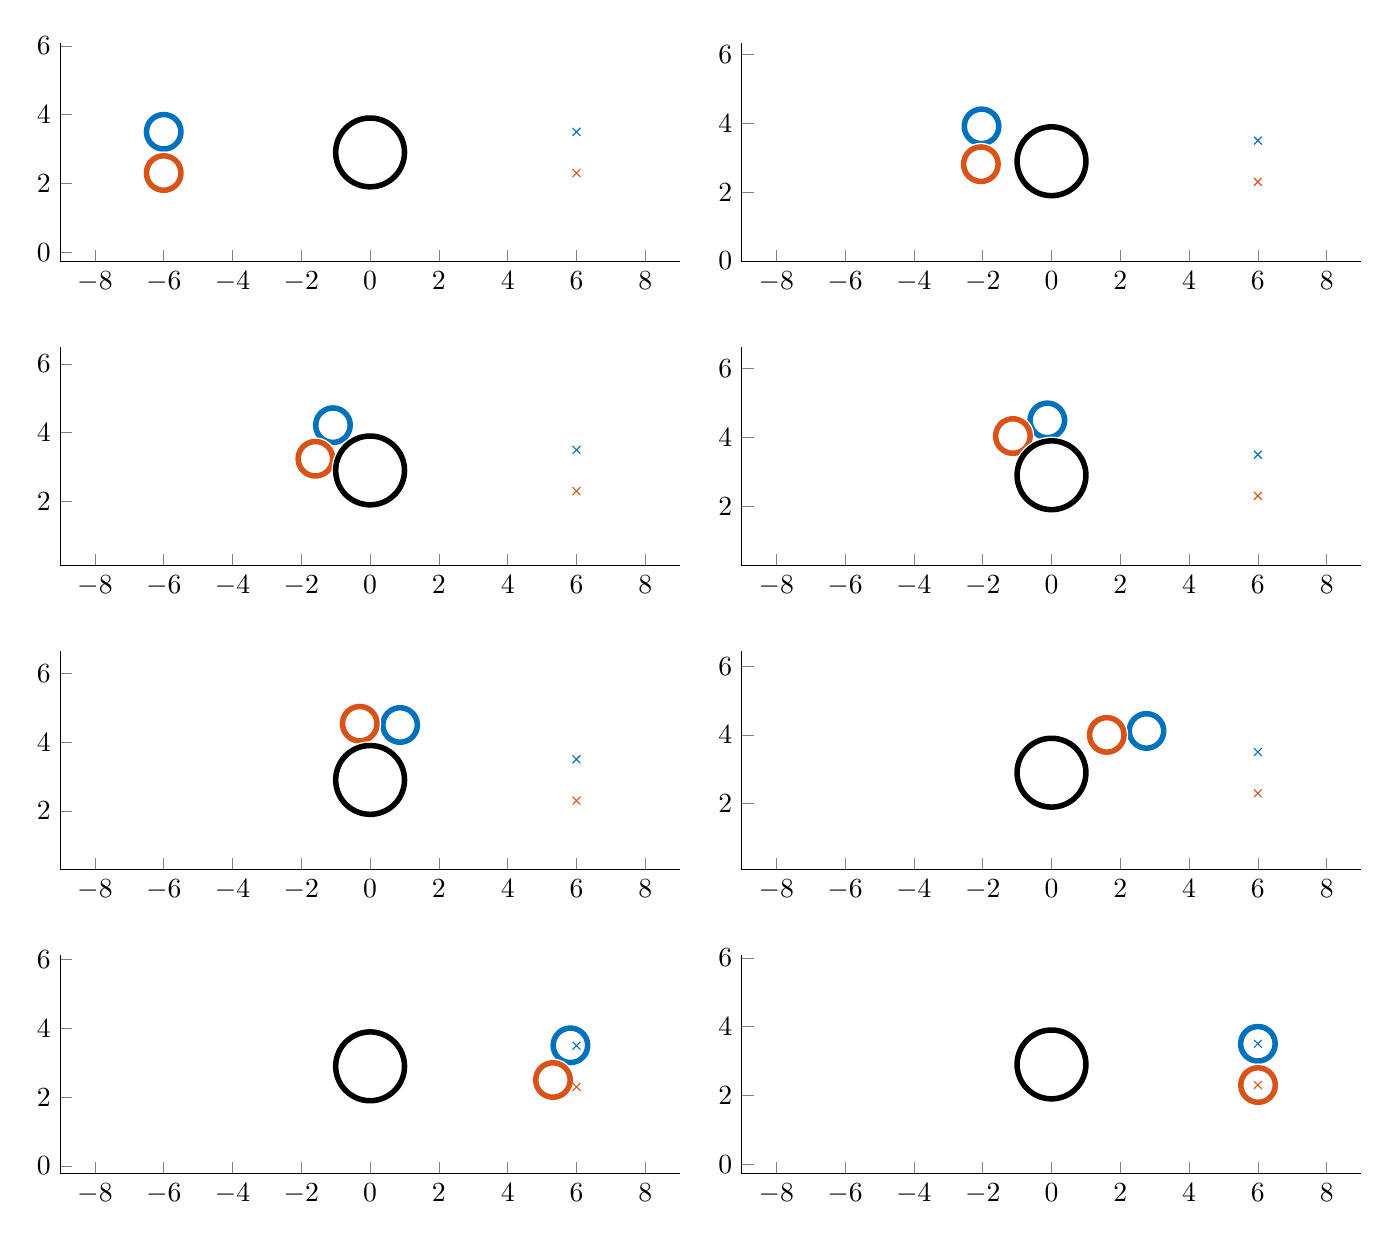
\begin{tikzpicture}

\definecolor{mycolor1}{rgb}{0.00000,0.44700,0.74100}%
\definecolor{mycolor2}{rgb}{0.85000,0.32500,0.09800}%
\definecolor{mycolor3}{rgb}{0.92900,0.69400,0.12500}%

\begin{axis}[%
width=3.096in,
height=1.094in,
at={(2.593in,5.323in)},
scale only axis,
unbounded coords=jump,
xmin=-9,
xmax=9,
%xmajorgrids,
ymin=-0.281620023002354,
ymax=6.08162002300235,
%ymajorgrids,
axis background/.style={fill=white},
axis x line*=bottom,
axis y line*=left
]
\addplot [color=mycolor1,only marks,mark=x,mark options={solid},forget plot]
  table[row sep=crcr]{%
6	3.5\\
};
\addplot [color=mycolor2,only marks,mark=x,mark options={solid},forget plot]
  table[row sep=crcr]{%
6	2.3\\
};
\addplot [color=white,solid,line width=3.0pt,forget plot]
  table[row sep=crcr]{%
-5.5	3.5\\
-5.50030458649045	3.51744974835125\\
-5.50121797487009	3.53487823687206\\
-5.50273905231586	3.55226423163383\\
-5.50486596562921	3.56958655048003\\
-5.5075961234939	3.58682408883347\\
-5.5109261996331	3.60395584540888\\
-5.514852136862	3.62096094779983\\
-5.51936915203084	3.6378186779085\\
-5.52447174185242	3.65450849718747\\
-5.53015368960705	3.67101007166283\\
-5.53640807271661	3.68730329670796\\
-5.5432272711787	3.7033683215379\\
-5.55060297685042	3.71918557339454\\
-5.55852620357054	3.73473578139295\\
-5.56698729810778	3.75\\
-5.57597595192179	3.7649596321166\\
-5.58548121372248	3.77959645173537\\
-5.59549150281253	3.79389262614624\\
-5.60599462319664	3.80783073766283\\
-5.61697777844051	3.82139380484327\\
-5.6284275872613	3.83456530317943\\
-5.64033009983067	3.8473291852295\\
-5.6526708147705	3.85966990016933\\
-5.66543469682057	3.8715724127387\\
-5.67860619515673	3.88302222155949\\
-5.69216926233717	3.89400537680336\\
-5.70610737385376	3.90450849718747\\
-5.72040354826463	3.91451878627752\\
-5.7350403678834	3.92402404807821\\
-5.75	3.93301270189222\\
-5.76526421860705	3.94147379642946\\
-5.78081442660546	3.94939702314958\\
-5.7966316784621	3.9567727288213\\
-5.81269670329204	3.96359192728339\\
-5.82898992833717	3.96984631039295\\
-5.84549150281253	3.97552825814758\\
-5.8621813220915	3.98063084796916\\
-5.87903905220017	3.985147863138\\
-5.89604415459112	3.9890738003669\\
-5.91317591116653	3.9924038765061\\
-5.93041344951997	3.99513403437079\\
-5.94773576836617	3.99726094768414\\
-5.96512176312794	3.99878202512991\\
-5.98255025164875	3.99969541350955\\
-6	4\\
-6.01744974835125	3.99969541350955\\
-6.03487823687206	3.99878202512991\\
-6.05226423163383	3.99726094768414\\
-6.06958655048003	3.99513403437079\\
-6.08682408883347	3.9924038765061\\
-6.10395584540888	3.9890738003669\\
-6.12096094779983	3.985147863138\\
-6.1378186779085	3.98063084796916\\
-6.15450849718747	3.97552825814758\\
-6.17101007166283	3.96984631039295\\
-6.18730329670796	3.96359192728339\\
-6.2033683215379	3.9567727288213\\
-6.21918557339454	3.94939702314958\\
-6.23473578139295	3.94147379642946\\
-6.25	3.93301270189222\\
-6.2649596321166	3.92402404807821\\
-6.27959645173537	3.91451878627752\\
-6.29389262614624	3.90450849718747\\
-6.30783073766283	3.89400537680336\\
-6.32139380484327	3.88302222155949\\
-6.33456530317943	3.8715724127387\\
-6.3473291852295	3.85966990016933\\
-6.35966990016933	3.8473291852295\\
-6.3715724127387	3.83456530317943\\
-6.38302222155949	3.82139380484327\\
-6.39400537680336	3.80783073766283\\
-6.40450849718747	3.79389262614624\\
-6.41451878627752	3.77959645173537\\
-6.42402404807821	3.7649596321166\\
-6.43301270189222	3.75\\
-6.44147379642946	3.73473578139295\\
-6.44939702314958	3.71918557339454\\
-6.4567727288213	3.7033683215379\\
-6.46359192728339	3.68730329670796\\
-6.46984631039295	3.67101007166283\\
-6.47552825814758	3.65450849718747\\
-6.48063084796916	3.6378186779085\\
-6.485147863138	3.62096094779983\\
-6.4890738003669	3.60395584540888\\
-6.4924038765061	3.58682408883347\\
-6.49513403437079	3.56958655048003\\
-6.49726094768414	3.55226423163383\\
-6.49878202512991	3.53487823687206\\
-6.49969541350955	3.51744974835125\\
-6.5	3.5\\
-6.49969541350955	3.48255025164875\\
-6.49878202512991	3.46512176312794\\
-6.49726094768414	3.44773576836617\\
-6.49513403437079	3.43041344951997\\
-6.4924038765061	3.41317591116653\\
-6.4890738003669	3.39604415459112\\
-6.485147863138	3.37903905220017\\
-6.48063084796916	3.3621813220915\\
-6.47552825814758	3.34549150281253\\
-6.46984631039295	3.32898992833717\\
-6.46359192728339	3.31269670329204\\
-6.4567727288213	3.2966316784621\\
-6.44939702314958	3.28081442660546\\
-6.44147379642946	3.26526421860705\\
-6.43301270189222	3.25\\
-6.42402404807821	3.2350403678834\\
-6.41451878627752	3.22040354826463\\
-6.40450849718747	3.20610737385376\\
-6.39400537680336	3.19216926233717\\
-6.38302222155949	3.17860619515673\\
-6.3715724127387	3.16543469682057\\
-6.35966990016933	3.1526708147705\\
-6.3473291852295	3.14033009983067\\
-6.33456530317943	3.1284275872613\\
-6.32139380484327	3.11697777844051\\
-6.30783073766283	3.10599462319664\\
-6.29389262614624	3.09549150281253\\
-6.27959645173537	3.08548121372248\\
-6.2649596321166	3.07597595192179\\
-6.25	3.06698729810778\\
-6.23473578139295	3.05852620357054\\
-6.21918557339454	3.05060297685042\\
-6.2033683215379	3.0432272711787\\
-6.18730329670796	3.03640807271661\\
-6.17101007166283	3.03015368960705\\
-6.15450849718747	3.02447174185242\\
-6.1378186779085	3.01936915203084\\
-6.12096094779983	3.014852136862\\
-6.10395584540888	3.0109261996331\\
-6.08682408883347	3.0075961234939\\
-6.06958655048003	3.00486596562921\\
-6.05226423163383	3.00273905231586\\
-6.03487823687206	3.00121797487009\\
-6.01744974835125	3.00030458649045\\
-6	3\\
-5.98255025164875	3.00030458649045\\
-5.96512176312794	3.00121797487009\\
-5.94773576836617	3.00273905231586\\
-5.93041344951997	3.00486596562921\\
-5.91317591116653	3.0075961234939\\
-5.89604415459112	3.0109261996331\\
-5.87903905220017	3.014852136862\\
-5.8621813220915	3.01936915203084\\
-5.84549150281253	3.02447174185242\\
-5.82898992833717	3.03015368960705\\
-5.81269670329204	3.03640807271661\\
-5.7966316784621	3.0432272711787\\
-5.78081442660546	3.05060297685042\\
-5.76526421860705	3.05852620357054\\
-5.75	3.06698729810778\\
-5.7350403678834	3.07597595192179\\
-5.72040354826463	3.08548121372248\\
-5.70610737385376	3.09549150281253\\
-5.69216926233717	3.10599462319664\\
-5.67860619515673	3.11697777844051\\
-5.66543469682057	3.1284275872613\\
-5.6526708147705	3.14033009983067\\
-5.64033009983067	3.1526708147705\\
-5.6284275872613	3.16543469682057\\
-5.61697777844051	3.17860619515673\\
-5.60599462319664	3.19216926233717\\
-5.59549150281253	3.20610737385376\\
-5.58548121372248	3.22040354826463\\
-5.57597595192179	3.2350403678834\\
-5.56698729810778	3.25\\
-5.55852620357054	3.26526421860705\\
-5.55060297685042	3.28081442660546\\
-5.5432272711787	3.2966316784621\\
-5.53640807271661	3.31269670329204\\
-5.53015368960705	3.32898992833717\\
-5.52447174185242	3.34549150281253\\
-5.51936915203084	3.3621813220915\\
-5.514852136862	3.37903905220017\\
-5.5109261996331	3.39604415459112\\
-5.5075961234939	3.41317591116653\\
-5.50486596562921	3.43041344951997\\
-5.50273905231586	3.44773576836617\\
-5.50121797487009	3.46512176312794\\
-5.50030458649045	3.48255025164875\\
-5.5	3.5\\
nan	nan\\
};
\addplot [color=mycolor1,solid,line width=2.0pt,forget plot]
  table[row sep=crcr]{%
-5.5	3.5\\
-5.50030458649045	3.51744974835125\\
-5.50121797487009	3.53487823687206\\
-5.50273905231586	3.55226423163383\\
-5.50486596562921	3.56958655048003\\
-5.5075961234939	3.58682408883347\\
-5.5109261996331	3.60395584540888\\
-5.514852136862	3.62096094779983\\
-5.51936915203084	3.6378186779085\\
-5.52447174185242	3.65450849718747\\
-5.53015368960705	3.67101007166283\\
-5.53640807271661	3.68730329670796\\
-5.5432272711787	3.7033683215379\\
-5.55060297685042	3.71918557339454\\
-5.55852620357054	3.73473578139295\\
-5.56698729810778	3.75\\
-5.57597595192179	3.7649596321166\\
-5.58548121372248	3.77959645173537\\
-5.59549150281253	3.79389262614624\\
-5.60599462319664	3.80783073766283\\
-5.61697777844051	3.82139380484327\\
-5.6284275872613	3.83456530317943\\
-5.64033009983067	3.8473291852295\\
-5.6526708147705	3.85966990016933\\
-5.66543469682057	3.8715724127387\\
-5.67860619515673	3.88302222155949\\
-5.69216926233717	3.89400537680336\\
-5.70610737385376	3.90450849718747\\
-5.72040354826463	3.91451878627752\\
-5.7350403678834	3.92402404807821\\
-5.75	3.93301270189222\\
-5.76526421860705	3.94147379642946\\
-5.78081442660546	3.94939702314958\\
-5.7966316784621	3.9567727288213\\
-5.81269670329204	3.96359192728339\\
-5.82898992833717	3.96984631039295\\
-5.84549150281253	3.97552825814758\\
-5.8621813220915	3.98063084796916\\
-5.87903905220017	3.985147863138\\
-5.89604415459112	3.9890738003669\\
-5.91317591116653	3.9924038765061\\
-5.93041344951997	3.99513403437079\\
-5.94773576836617	3.99726094768414\\
-5.96512176312794	3.99878202512991\\
-5.98255025164875	3.99969541350955\\
-6	4\\
-6.01744974835125	3.99969541350955\\
-6.03487823687206	3.99878202512991\\
-6.05226423163383	3.99726094768414\\
-6.06958655048003	3.99513403437079\\
-6.08682408883347	3.9924038765061\\
-6.10395584540888	3.9890738003669\\
-6.12096094779983	3.985147863138\\
-6.1378186779085	3.98063084796916\\
-6.15450849718747	3.97552825814758\\
-6.17101007166283	3.96984631039295\\
-6.18730329670796	3.96359192728339\\
-6.2033683215379	3.9567727288213\\
-6.21918557339454	3.94939702314958\\
-6.23473578139295	3.94147379642946\\
-6.25	3.93301270189222\\
-6.2649596321166	3.92402404807821\\
-6.27959645173537	3.91451878627752\\
-6.29389262614624	3.90450849718747\\
-6.30783073766283	3.89400537680336\\
-6.32139380484327	3.88302222155949\\
-6.33456530317943	3.8715724127387\\
-6.3473291852295	3.85966990016933\\
-6.35966990016933	3.8473291852295\\
-6.3715724127387	3.83456530317943\\
-6.38302222155949	3.82139380484327\\
-6.39400537680336	3.80783073766283\\
-6.40450849718747	3.79389262614624\\
-6.41451878627752	3.77959645173537\\
-6.42402404807821	3.7649596321166\\
-6.43301270189222	3.75\\
-6.44147379642946	3.73473578139295\\
-6.44939702314958	3.71918557339454\\
-6.4567727288213	3.7033683215379\\
-6.46359192728339	3.68730329670796\\
-6.46984631039295	3.67101007166283\\
-6.47552825814758	3.65450849718747\\
-6.48063084796916	3.6378186779085\\
-6.485147863138	3.62096094779983\\
-6.4890738003669	3.60395584540888\\
-6.4924038765061	3.58682408883347\\
-6.49513403437079	3.56958655048003\\
-6.49726094768414	3.55226423163383\\
-6.49878202512991	3.53487823687206\\
-6.49969541350955	3.51744974835125\\
-6.5	3.5\\
-6.49969541350955	3.48255025164875\\
-6.49878202512991	3.46512176312794\\
-6.49726094768414	3.44773576836617\\
-6.49513403437079	3.43041344951997\\
-6.4924038765061	3.41317591116653\\
-6.4890738003669	3.39604415459112\\
-6.485147863138	3.37903905220017\\
-6.48063084796916	3.3621813220915\\
-6.47552825814758	3.34549150281253\\
-6.46984631039295	3.32898992833717\\
-6.46359192728339	3.31269670329204\\
-6.4567727288213	3.2966316784621\\
-6.44939702314958	3.28081442660546\\
-6.44147379642946	3.26526421860705\\
-6.43301270189222	3.25\\
-6.42402404807821	3.2350403678834\\
-6.41451878627752	3.22040354826463\\
-6.40450849718747	3.20610737385376\\
-6.39400537680336	3.19216926233717\\
-6.38302222155949	3.17860619515673\\
-6.3715724127387	3.16543469682057\\
-6.35966990016933	3.1526708147705\\
-6.3473291852295	3.14033009983067\\
-6.33456530317943	3.1284275872613\\
-6.32139380484327	3.11697777844051\\
-6.30783073766283	3.10599462319664\\
-6.29389262614624	3.09549150281253\\
-6.27959645173537	3.08548121372248\\
-6.2649596321166	3.07597595192179\\
-6.25	3.06698729810778\\
-6.23473578139295	3.05852620357054\\
-6.21918557339454	3.05060297685042\\
-6.2033683215379	3.0432272711787\\
-6.18730329670796	3.03640807271661\\
-6.17101007166283	3.03015368960705\\
-6.15450849718747	3.02447174185242\\
-6.1378186779085	3.01936915203084\\
-6.12096094779983	3.014852136862\\
-6.10395584540888	3.0109261996331\\
-6.08682408883347	3.0075961234939\\
-6.06958655048003	3.00486596562921\\
-6.05226423163383	3.00273905231586\\
-6.03487823687206	3.00121797487009\\
-6.01744974835125	3.00030458649045\\
-6	3\\
-5.98255025164875	3.00030458649045\\
-5.96512176312794	3.00121797487009\\
-5.94773576836617	3.00273905231586\\
-5.93041344951997	3.00486596562921\\
-5.91317591116653	3.0075961234939\\
-5.89604415459112	3.0109261996331\\
-5.87903905220017	3.014852136862\\
-5.8621813220915	3.01936915203084\\
-5.84549150281253	3.02447174185242\\
-5.82898992833717	3.03015368960705\\
-5.81269670329204	3.03640807271661\\
-5.7966316784621	3.0432272711787\\
-5.78081442660546	3.05060297685042\\
-5.76526421860705	3.05852620357054\\
-5.75	3.06698729810778\\
-5.7350403678834	3.07597595192179\\
-5.72040354826463	3.08548121372248\\
-5.70610737385376	3.09549150281253\\
-5.69216926233717	3.10599462319664\\
-5.67860619515673	3.11697777844051\\
-5.66543469682057	3.1284275872613\\
-5.6526708147705	3.14033009983067\\
-5.64033009983067	3.1526708147705\\
-5.6284275872613	3.16543469682057\\
-5.61697777844051	3.17860619515673\\
-5.60599462319664	3.19216926233717\\
-5.59549150281253	3.20610737385376\\
-5.58548121372248	3.22040354826463\\
-5.57597595192179	3.2350403678834\\
-5.56698729810778	3.25\\
-5.55852620357054	3.26526421860705\\
-5.55060297685042	3.28081442660546\\
-5.5432272711787	3.2966316784621\\
-5.53640807271661	3.31269670329204\\
-5.53015368960705	3.32898992833717\\
-5.52447174185242	3.34549150281253\\
-5.51936915203084	3.3621813220915\\
-5.514852136862	3.37903905220017\\
-5.5109261996331	3.39604415459112\\
-5.5075961234939	3.41317591116653\\
-5.50486596562921	3.43041344951997\\
-5.50273905231586	3.44773576836617\\
-5.50121797487009	3.46512176312794\\
-5.50030458649045	3.48255025164875\\
-5.5	3.5\\
nan	nan\\
};
\addplot [color=white,solid,line width=3.0pt,forget plot]
  table[row sep=crcr]{%
-5.5	2.3\\
-5.50030458649045	2.31744974835125\\
-5.50121797487009	2.33487823687206\\
-5.50273905231586	2.35226423163383\\
-5.50486596562921	2.36958655048003\\
-5.5075961234939	2.38682408883346\\
-5.5109261996331	2.40395584540888\\
-5.514852136862	2.42096094779983\\
-5.51936915203084	2.4378186779085\\
-5.52447174185242	2.45450849718747\\
-5.53015368960705	2.47101007166283\\
-5.53640807271661	2.48730329670796\\
-5.5432272711787	2.5033683215379\\
-5.55060297685042	2.51918557339454\\
-5.55852620357054	2.53473578139295\\
-5.56698729810778	2.55\\
-5.57597595192179	2.5649596321166\\
-5.58548121372248	2.57959645173537\\
-5.59549150281253	2.59389262614624\\
-5.60599462319664	2.60783073766283\\
-5.61697777844051	2.62139380484327\\
-5.6284275872613	2.63456530317943\\
-5.64033009983067	2.6473291852295\\
-5.6526708147705	2.65966990016933\\
-5.66543469682057	2.6715724127387\\
-5.67860619515673	2.68302222155949\\
-5.69216926233717	2.69400537680336\\
-5.70610737385376	2.70450849718747\\
-5.72040354826463	2.71451878627752\\
-5.7350403678834	2.72402404807821\\
-5.75	2.73301270189222\\
-5.76526421860705	2.74147379642946\\
-5.78081442660546	2.74939702314958\\
-5.7966316784621	2.7567727288213\\
-5.81269670329204	2.76359192728339\\
-5.82898992833717	2.76984631039295\\
-5.84549150281253	2.77552825814758\\
-5.8621813220915	2.78063084796916\\
-5.87903905220017	2.785147863138\\
-5.89604415459112	2.7890738003669\\
-5.91317591116653	2.7924038765061\\
-5.93041344951997	2.79513403437078\\
-5.94773576836617	2.79726094768414\\
-5.96512176312794	2.79878202512991\\
-5.98255025164875	2.79969541350955\\
-6	2.8\\
-6.01744974835125	2.79969541350955\\
-6.03487823687206	2.79878202512991\\
-6.05226423163383	2.79726094768414\\
-6.06958655048003	2.79513403437078\\
-6.08682408883347	2.7924038765061\\
-6.10395584540888	2.7890738003669\\
-6.12096094779983	2.785147863138\\
-6.1378186779085	2.78063084796916\\
-6.15450849718747	2.77552825814758\\
-6.17101007166283	2.76984631039295\\
-6.18730329670796	2.76359192728339\\
-6.2033683215379	2.7567727288213\\
-6.21918557339454	2.74939702314958\\
-6.23473578139295	2.74147379642946\\
-6.25	2.73301270189222\\
-6.2649596321166	2.72402404807821\\
-6.27959645173537	2.71451878627752\\
-6.29389262614624	2.70450849718747\\
-6.30783073766283	2.69400537680336\\
-6.32139380484327	2.68302222155949\\
-6.33456530317943	2.6715724127387\\
-6.3473291852295	2.65966990016933\\
-6.35966990016933	2.6473291852295\\
-6.3715724127387	2.63456530317943\\
-6.38302222155949	2.62139380484327\\
-6.39400537680336	2.60783073766283\\
-6.40450849718747	2.59389262614624\\
-6.41451878627752	2.57959645173537\\
-6.42402404807821	2.5649596321166\\
-6.43301270189222	2.55\\
-6.44147379642946	2.53473578139295\\
-6.44939702314958	2.51918557339454\\
-6.4567727288213	2.5033683215379\\
-6.46359192728339	2.48730329670796\\
-6.46984631039295	2.47101007166283\\
-6.47552825814758	2.45450849718747\\
-6.48063084796916	2.4378186779085\\
-6.485147863138	2.42096094779983\\
-6.4890738003669	2.40395584540888\\
-6.4924038765061	2.38682408883346\\
-6.49513403437079	2.36958655048003\\
-6.49726094768414	2.35226423163383\\
-6.49878202512991	2.33487823687206\\
-6.49969541350955	2.31744974835125\\
-6.5	2.3\\
-6.49969541350955	2.28255025164875\\
-6.49878202512991	2.26512176312794\\
-6.49726094768414	2.24773576836617\\
-6.49513403437079	2.23041344951997\\
-6.4924038765061	2.21317591116653\\
-6.4890738003669	2.19604415459112\\
-6.485147863138	2.17903905220017\\
-6.48063084796916	2.1621813220915\\
-6.47552825814758	2.14549150281253\\
-6.46984631039295	2.12898992833717\\
-6.46359192728339	2.11269670329204\\
-6.4567727288213	2.0966316784621\\
-6.44939702314958	2.08081442660546\\
-6.44147379642946	2.06526421860705\\
-6.43301270189222	2.05\\
-6.42402404807821	2.0350403678834\\
-6.41451878627752	2.02040354826463\\
-6.40450849718747	2.00610737385376\\
-6.39400537680336	1.99216926233717\\
-6.38302222155949	1.97860619515673\\
-6.3715724127387	1.96543469682057\\
-6.35966990016933	1.9526708147705\\
-6.3473291852295	1.94033009983067\\
-6.33456530317943	1.9284275872613\\
-6.32139380484327	1.91697777844051\\
-6.30783073766283	1.90599462319664\\
-6.29389262614624	1.89549150281253\\
-6.27959645173537	1.88548121372248\\
-6.2649596321166	1.87597595192179\\
-6.25	1.86698729810778\\
-6.23473578139295	1.85852620357054\\
-6.21918557339454	1.85060297685042\\
-6.2033683215379	1.8432272711787\\
-6.18730329670796	1.83640807271661\\
-6.17101007166283	1.83015368960705\\
-6.15450849718747	1.82447174185242\\
-6.1378186779085	1.81936915203084\\
-6.12096094779983	1.814852136862\\
-6.10395584540888	1.8109261996331\\
-6.08682408883347	1.8075961234939\\
-6.06958655048003	1.80486596562921\\
-6.05226423163383	1.80273905231586\\
-6.03487823687206	1.80121797487009\\
-6.01744974835125	1.80030458649045\\
-6	1.8\\
-5.98255025164875	1.80030458649045\\
-5.96512176312794	1.80121797487009\\
-5.94773576836617	1.80273905231586\\
-5.93041344951997	1.80486596562921\\
-5.91317591116653	1.8075961234939\\
-5.89604415459112	1.8109261996331\\
-5.87903905220017	1.814852136862\\
-5.8621813220915	1.81936915203084\\
-5.84549150281253	1.82447174185242\\
-5.82898992833717	1.83015368960705\\
-5.81269670329204	1.83640807271661\\
-5.7966316784621	1.8432272711787\\
-5.78081442660546	1.85060297685042\\
-5.76526421860705	1.85852620357054\\
-5.75	1.86698729810778\\
-5.7350403678834	1.87597595192179\\
-5.72040354826463	1.88548121372248\\
-5.70610737385376	1.89549150281253\\
-5.69216926233717	1.90599462319664\\
-5.67860619515673	1.91697777844051\\
-5.66543469682057	1.9284275872613\\
-5.6526708147705	1.94033009983067\\
-5.64033009983067	1.9526708147705\\
-5.6284275872613	1.96543469682057\\
-5.61697777844051	1.97860619515673\\
-5.60599462319664	1.99216926233717\\
-5.59549150281253	2.00610737385376\\
-5.58548121372248	2.02040354826463\\
-5.57597595192179	2.0350403678834\\
-5.56698729810778	2.05\\
-5.55852620357054	2.06526421860705\\
-5.55060297685042	2.08081442660546\\
-5.5432272711787	2.0966316784621\\
-5.53640807271661	2.11269670329204\\
-5.53015368960705	2.12898992833717\\
-5.52447174185242	2.14549150281253\\
-5.51936915203084	2.1621813220915\\
-5.514852136862	2.17903905220017\\
-5.5109261996331	2.19604415459112\\
-5.5075961234939	2.21317591116653\\
-5.50486596562921	2.23041344951997\\
-5.50273905231586	2.24773576836617\\
-5.50121797487009	2.26512176312794\\
-5.50030458649045	2.28255025164875\\
-5.5	2.3\\
nan	nan\\
};
\addplot [color=mycolor2,solid,line width=2.0pt,forget plot]
  table[row sep=crcr]{%
-5.5	2.3\\
-5.50030458649045	2.31744974835125\\
-5.50121797487009	2.33487823687206\\
-5.50273905231586	2.35226423163383\\
-5.50486596562921	2.36958655048003\\
-5.5075961234939	2.38682408883346\\
-5.5109261996331	2.40395584540888\\
-5.514852136862	2.42096094779983\\
-5.51936915203084	2.4378186779085\\
-5.52447174185242	2.45450849718747\\
-5.53015368960705	2.47101007166283\\
-5.53640807271661	2.48730329670796\\
-5.5432272711787	2.5033683215379\\
-5.55060297685042	2.51918557339454\\
-5.55852620357054	2.53473578139295\\
-5.56698729810778	2.55\\
-5.57597595192179	2.5649596321166\\
-5.58548121372248	2.57959645173537\\
-5.59549150281253	2.59389262614624\\
-5.60599462319664	2.60783073766283\\
-5.61697777844051	2.62139380484327\\
-5.6284275872613	2.63456530317943\\
-5.64033009983067	2.6473291852295\\
-5.6526708147705	2.65966990016933\\
-5.66543469682057	2.6715724127387\\
-5.67860619515673	2.68302222155949\\
-5.69216926233717	2.69400537680336\\
-5.70610737385376	2.70450849718747\\
-5.72040354826463	2.71451878627752\\
-5.7350403678834	2.72402404807821\\
-5.75	2.73301270189222\\
-5.76526421860705	2.74147379642946\\
-5.78081442660546	2.74939702314958\\
-5.7966316784621	2.7567727288213\\
-5.81269670329204	2.76359192728339\\
-5.82898992833717	2.76984631039295\\
-5.84549150281253	2.77552825814758\\
-5.8621813220915	2.78063084796916\\
-5.87903905220017	2.785147863138\\
-5.89604415459112	2.7890738003669\\
-5.91317591116653	2.7924038765061\\
-5.93041344951997	2.79513403437078\\
-5.94773576836617	2.79726094768414\\
-5.96512176312794	2.79878202512991\\
-5.98255025164875	2.79969541350955\\
-6	2.8\\
-6.01744974835125	2.79969541350955\\
-6.03487823687206	2.79878202512991\\
-6.05226423163383	2.79726094768414\\
-6.06958655048003	2.79513403437078\\
-6.08682408883347	2.7924038765061\\
-6.10395584540888	2.7890738003669\\
-6.12096094779983	2.785147863138\\
-6.1378186779085	2.78063084796916\\
-6.15450849718747	2.77552825814758\\
-6.17101007166283	2.76984631039295\\
-6.18730329670796	2.76359192728339\\
-6.2033683215379	2.7567727288213\\
-6.21918557339454	2.74939702314958\\
-6.23473578139295	2.74147379642946\\
-6.25	2.73301270189222\\
-6.2649596321166	2.72402404807821\\
-6.27959645173537	2.71451878627752\\
-6.29389262614624	2.70450849718747\\
-6.30783073766283	2.69400537680336\\
-6.32139380484327	2.68302222155949\\
-6.33456530317943	2.6715724127387\\
-6.3473291852295	2.65966990016933\\
-6.35966990016933	2.6473291852295\\
-6.3715724127387	2.63456530317943\\
-6.38302222155949	2.62139380484327\\
-6.39400537680336	2.60783073766283\\
-6.40450849718747	2.59389262614624\\
-6.41451878627752	2.57959645173537\\
-6.42402404807821	2.5649596321166\\
-6.43301270189222	2.55\\
-6.44147379642946	2.53473578139295\\
-6.44939702314958	2.51918557339454\\
-6.4567727288213	2.5033683215379\\
-6.46359192728339	2.48730329670796\\
-6.46984631039295	2.47101007166283\\
-6.47552825814758	2.45450849718747\\
-6.48063084796916	2.4378186779085\\
-6.485147863138	2.42096094779983\\
-6.4890738003669	2.40395584540888\\
-6.4924038765061	2.38682408883346\\
-6.49513403437079	2.36958655048003\\
-6.49726094768414	2.35226423163383\\
-6.49878202512991	2.33487823687206\\
-6.49969541350955	2.31744974835125\\
-6.5	2.3\\
-6.49969541350955	2.28255025164875\\
-6.49878202512991	2.26512176312794\\
-6.49726094768414	2.24773576836617\\
-6.49513403437079	2.23041344951997\\
-6.4924038765061	2.21317591116653\\
-6.4890738003669	2.19604415459112\\
-6.485147863138	2.17903905220017\\
-6.48063084796916	2.1621813220915\\
-6.47552825814758	2.14549150281253\\
-6.46984631039295	2.12898992833717\\
-6.46359192728339	2.11269670329204\\
-6.4567727288213	2.0966316784621\\
-6.44939702314958	2.08081442660546\\
-6.44147379642946	2.06526421860705\\
-6.43301270189222	2.05\\
-6.42402404807821	2.0350403678834\\
-6.41451878627752	2.02040354826463\\
-6.40450849718747	2.00610737385376\\
-6.39400537680336	1.99216926233717\\
-6.38302222155949	1.97860619515673\\
-6.3715724127387	1.96543469682057\\
-6.35966990016933	1.9526708147705\\
-6.3473291852295	1.94033009983067\\
-6.33456530317943	1.9284275872613\\
-6.32139380484327	1.91697777844051\\
-6.30783073766283	1.90599462319664\\
-6.29389262614624	1.89549150281253\\
-6.27959645173537	1.88548121372248\\
-6.2649596321166	1.87597595192179\\
-6.25	1.86698729810778\\
-6.23473578139295	1.85852620357054\\
-6.21918557339454	1.85060297685042\\
-6.2033683215379	1.8432272711787\\
-6.18730329670796	1.83640807271661\\
-6.17101007166283	1.83015368960705\\
-6.15450849718747	1.82447174185242\\
-6.1378186779085	1.81936915203084\\
-6.12096094779983	1.814852136862\\
-6.10395584540888	1.8109261996331\\
-6.08682408883347	1.8075961234939\\
-6.06958655048003	1.80486596562921\\
-6.05226423163383	1.80273905231586\\
-6.03487823687206	1.80121797487009\\
-6.01744974835125	1.80030458649045\\
-6	1.8\\
-5.98255025164875	1.80030458649045\\
-5.96512176312794	1.80121797487009\\
-5.94773576836617	1.80273905231586\\
-5.93041344951997	1.80486596562921\\
-5.91317591116653	1.8075961234939\\
-5.89604415459112	1.8109261996331\\
-5.87903905220017	1.814852136862\\
-5.8621813220915	1.81936915203084\\
-5.84549150281253	1.82447174185242\\
-5.82898992833717	1.83015368960705\\
-5.81269670329204	1.83640807271661\\
-5.7966316784621	1.8432272711787\\
-5.78081442660546	1.85060297685042\\
-5.76526421860705	1.85852620357054\\
-5.75	1.86698729810778\\
-5.7350403678834	1.87597595192179\\
-5.72040354826463	1.88548121372248\\
-5.70610737385376	1.89549150281253\\
-5.69216926233717	1.90599462319664\\
-5.67860619515673	1.91697777844051\\
-5.66543469682057	1.9284275872613\\
-5.6526708147705	1.94033009983067\\
-5.64033009983067	1.9526708147705\\
-5.6284275872613	1.96543469682057\\
-5.61697777844051	1.97860619515673\\
-5.60599462319664	1.99216926233717\\
-5.59549150281253	2.00610737385376\\
-5.58548121372248	2.02040354826463\\
-5.57597595192179	2.0350403678834\\
-5.56698729810778	2.05\\
-5.55852620357054	2.06526421860705\\
-5.55060297685042	2.08081442660546\\
-5.5432272711787	2.0966316784621\\
-5.53640807271661	2.11269670329204\\
-5.53015368960705	2.12898992833717\\
-5.52447174185242	2.14549150281253\\
-5.51936915203084	2.1621813220915\\
-5.514852136862	2.17903905220017\\
-5.5109261996331	2.19604415459112\\
-5.5075961234939	2.21317591116653\\
-5.50486596562921	2.23041344951997\\
-5.50273905231586	2.24773576836617\\
-5.50121797487009	2.26512176312794\\
-5.50030458649045	2.28255025164875\\
-5.5	2.3\\
nan	nan\\
};
\addplot [color=white,solid,line width=3.0pt,forget plot]
  table[row sep=crcr]{%
1	2.9\\
0.999390827019096	2.9348994967025\\
0.997564050259824	2.96975647374413\\
0.994521895368273	3.00452846326765\\
0.99026806874157	3.03917310096007\\
0.984807753012208	3.07364817766693\\
0.978147600733806	3.10791169081776\\
0.970295726275996	3.14192189559967\\
0.961261695938319	3.175637355817\\
0.951056516295154	3.20901699437495\\
0.939692620785908	3.24202014332567\\
0.927183854566787	3.27460659341591\\
0.913545457642601	3.3067366430758\\
0.898794046299167	3.33837114678908\\
0.882947592858927	3.36947156278589\\
0.866025403784439	3.4\\
0.848048096156426	3.42991926423321\\
0.829037572555042	3.45919290347075\\
0.809016994374947	3.48778525229247\\
0.788010753606722	3.51566147532566\\
0.766044443118978	3.54278760968654\\
0.743144825477394	3.56913060635886\\
0.719339800338651	3.594658370459\\
0.694658370458997	3.61933980033865\\
0.669130606358858	3.64314482547739\\
0.642787609686539	3.66604444311898\\
0.615661475325658	3.68801075360672\\
0.587785252292473	3.70901699437495\\
0.559192903470747	3.72903757255504\\
0.529919264233205	3.74804809615643\\
0.5	3.76602540378444\\
0.469471562785891	3.78294759285893\\
0.438371146789077	3.79879404629917\\
0.4067366430758	3.8135454576426\\
0.374606593415912	3.82718385456679\\
0.342020143325669	3.83969262078591\\
0.309016994374947	3.85105651629515\\
0.275637355816999	3.86126169593832\\
0.241921895599668	3.870295726276\\
0.207911690817759	3.87814760073381\\
0.17364817766693	3.88480775301221\\
0.139173100960066	3.89026806874157\\
0.104528463267653	3.89452189536827\\
0.0697564737441255	3.89756405025982\\
0.0348994967025011	3.8993908270191\\
6.12323399573677e-17	3.9\\
-0.0348994967025007	3.8993908270191\\
-0.0697564737441253	3.89756405025982\\
-0.104528463267653	3.89452189536827\\
-0.139173100960065	3.89026806874157\\
-0.17364817766693	3.88480775301221\\
-0.207911690817759	3.87814760073381\\
-0.241921895599668	3.870295726276\\
-0.275637355816999	3.86126169593832\\
-0.309016994374947	3.85105651629515\\
-0.342020143325669	3.83969262078591\\
-0.374606593415912	3.82718385456679\\
-0.4067366430758	3.8135454576426\\
-0.438371146789078	3.79879404629917\\
-0.469471562785891	3.78294759285893\\
-0.5	3.76602540378444\\
-0.529919264233205	3.74804809615643\\
-0.559192903470747	3.72903757255504\\
-0.587785252292473	3.70901699437495\\
-0.615661475325658	3.68801075360672\\
-0.642787609686539	3.66604444311898\\
-0.669130606358858	3.64314482547739\\
-0.694658370458997	3.61933980033865\\
-0.719339800338651	3.594658370459\\
-0.743144825477394	3.56913060635886\\
-0.766044443118978	3.54278760968654\\
-0.788010753606722	3.51566147532566\\
-0.809016994374947	3.48778525229247\\
-0.829037572555042	3.45919290347075\\
-0.848048096156426	3.42991926423321\\
-0.866025403784439	3.4\\
-0.882947592858927	3.36947156278589\\
-0.898794046299167	3.33837114678908\\
-0.913545457642601	3.3067366430758\\
-0.927183854566787	3.27460659341591\\
-0.939692620785908	3.24202014332567\\
-0.951056516295154	3.20901699437495\\
-0.961261695938319	3.175637355817\\
-0.970295726275996	3.14192189559967\\
-0.978147600733806	3.10791169081776\\
-0.984807753012208	3.07364817766693\\
-0.99026806874157	3.03917310096007\\
-0.994521895368273	3.00452846326765\\
-0.997564050259824	2.96975647374413\\
-0.999390827019096	2.9348994967025\\
-1	2.9\\
-0.999390827019096	2.8651005032975\\
-0.997564050259824	2.83024352625588\\
-0.994521895368273	2.79547153673235\\
-0.99026806874157	2.76082689903993\\
-0.984807753012208	2.72635182233307\\
-0.978147600733806	2.69208830918224\\
-0.970295726275997	2.65807810440033\\
-0.961261695938319	2.624362644183\\
-0.951056516295154	2.59098300562505\\
-0.939692620785908	2.55797985667433\\
-0.927183854566787	2.52539340658409\\
-0.913545457642601	2.4932633569242\\
-0.898794046299167	2.46162885321092\\
-0.882947592858927	2.43052843721411\\
-0.866025403784439	2.4\\
-0.848048096156426	2.3700807357668\\
-0.829037572555042	2.34080709652925\\
-0.809016994374947	2.31221474770753\\
-0.788010753606722	2.28433852467434\\
-0.766044443118978	2.25721239031346\\
-0.743144825477394	2.23086939364114\\
-0.719339800338651	2.205341629541\\
-0.694658370458997	2.18066019966135\\
-0.669130606358858	2.15685517452261\\
-0.642787609686539	2.13395555688102\\
-0.615661475325658	2.11198924639328\\
-0.587785252292473	2.09098300562505\\
-0.559192903470747	2.07096242744496\\
-0.529919264233205	2.05195190384357\\
-0.5	2.03397459621556\\
-0.469471562785891	2.01705240714107\\
-0.438371146789078	2.00120595370083\\
-0.4067366430758	1.9864545423574\\
-0.374606593415912	1.97281614543321\\
-0.342020143325669	1.96030737921409\\
-0.309016994374948	1.94894348370485\\
-0.275637355816999	1.93873830406168\\
-0.241921895599668	1.929704273724\\
-0.20791169081776	1.92185239926619\\
-0.17364817766693	1.91519224698779\\
-0.139173100960065	1.90973193125843\\
-0.104528463267653	1.90547810463173\\
-0.0697564737441256	1.90243594974018\\
-0.0348994967025016	1.9006091729809\\
-1.83697019872103e-16	1.9\\
0.0348994967025013	1.9006091729809\\
0.0697564737441252	1.90243594974018\\
0.104528463267653	1.90547810463173\\
0.139173100960065	1.90973193125843\\
0.17364817766693	1.91519224698779\\
0.207911690817759	1.92185239926619\\
0.241921895599667	1.929704273724\\
0.275637355816999	1.93873830406168\\
0.309016994374947	1.94894348370485\\
0.342020143325668	1.96030737921409\\
0.374606593415912	1.97281614543321\\
0.406736643075801	1.9864545423574\\
0.438371146789077	2.00120595370083\\
0.46947156278589	2.01705240714107\\
0.5	2.03397459621556\\
0.529919264233205	2.05195190384357\\
0.559192903470746	2.07096242744496\\
0.587785252292473	2.09098300562505\\
0.615661475325659	2.11198924639328\\
0.642787609686539	2.13395555688102\\
0.669130606358858	2.15685517452261\\
0.694658370458997	2.18066019966135\\
0.719339800338651	2.205341629541\\
0.743144825477394	2.23086939364114\\
0.766044443118978	2.25721239031346\\
0.788010753606722	2.28433852467434\\
0.809016994374947	2.31221474770753\\
0.829037572555041	2.34080709652925\\
0.848048096156425	2.37008073576679\\
0.866025403784438	2.4\\
0.882947592858927	2.43052843721411\\
0.898794046299167	2.46162885321092\\
0.913545457642601	2.4932633569242\\
0.927183854566787	2.52539340658409\\
0.939692620785908	2.55797985667433\\
0.951056516295154	2.59098300562505\\
0.961261695938319	2.624362644183\\
0.970295726275996	2.65807810440033\\
0.978147600733806	2.69208830918224\\
0.984807753012208	2.72635182233307\\
0.99026806874157	2.76082689903993\\
0.994521895368273	2.79547153673235\\
0.997564050259824	2.83024352625588\\
0.999390827019096	2.8651005032975\\
1	2.9\\
nan	nan\\
};
\addplot [color=black,solid,line width=2.0pt,forget plot]
  table[row sep=crcr]{%
1	2.9\\
0.999390827019096	2.9348994967025\\
0.997564050259824	2.96975647374413\\
0.994521895368273	3.00452846326765\\
0.99026806874157	3.03917310096007\\
0.984807753012208	3.07364817766693\\
0.978147600733806	3.10791169081776\\
0.970295726275996	3.14192189559967\\
0.961261695938319	3.175637355817\\
0.951056516295154	3.20901699437495\\
0.939692620785908	3.24202014332567\\
0.927183854566787	3.27460659341591\\
0.913545457642601	3.3067366430758\\
0.898794046299167	3.33837114678908\\
0.882947592858927	3.36947156278589\\
0.866025403784439	3.4\\
0.848048096156426	3.42991926423321\\
0.829037572555042	3.45919290347075\\
0.809016994374947	3.48778525229247\\
0.788010753606722	3.51566147532566\\
0.766044443118978	3.54278760968654\\
0.743144825477394	3.56913060635886\\
0.719339800338651	3.594658370459\\
0.694658370458997	3.61933980033865\\
0.669130606358858	3.64314482547739\\
0.642787609686539	3.66604444311898\\
0.615661475325658	3.68801075360672\\
0.587785252292473	3.70901699437495\\
0.559192903470747	3.72903757255504\\
0.529919264233205	3.74804809615643\\
0.5	3.76602540378444\\
0.469471562785891	3.78294759285893\\
0.438371146789077	3.79879404629917\\
0.4067366430758	3.8135454576426\\
0.374606593415912	3.82718385456679\\
0.342020143325669	3.83969262078591\\
0.309016994374947	3.85105651629515\\
0.275637355816999	3.86126169593832\\
0.241921895599668	3.870295726276\\
0.207911690817759	3.87814760073381\\
0.17364817766693	3.88480775301221\\
0.139173100960066	3.89026806874157\\
0.104528463267653	3.89452189536827\\
0.0697564737441255	3.89756405025982\\
0.0348994967025011	3.8993908270191\\
6.12323399573677e-17	3.9\\
-0.0348994967025007	3.8993908270191\\
-0.0697564737441253	3.89756405025982\\
-0.104528463267653	3.89452189536827\\
-0.139173100960065	3.89026806874157\\
-0.17364817766693	3.88480775301221\\
-0.207911690817759	3.87814760073381\\
-0.241921895599668	3.870295726276\\
-0.275637355816999	3.86126169593832\\
-0.309016994374947	3.85105651629515\\
-0.342020143325669	3.83969262078591\\
-0.374606593415912	3.82718385456679\\
-0.4067366430758	3.8135454576426\\
-0.438371146789078	3.79879404629917\\
-0.469471562785891	3.78294759285893\\
-0.5	3.76602540378444\\
-0.529919264233205	3.74804809615643\\
-0.559192903470747	3.72903757255504\\
-0.587785252292473	3.70901699437495\\
-0.615661475325658	3.68801075360672\\
-0.642787609686539	3.66604444311898\\
-0.669130606358858	3.64314482547739\\
-0.694658370458997	3.61933980033865\\
-0.719339800338651	3.594658370459\\
-0.743144825477394	3.56913060635886\\
-0.766044443118978	3.54278760968654\\
-0.788010753606722	3.51566147532566\\
-0.809016994374947	3.48778525229247\\
-0.829037572555042	3.45919290347075\\
-0.848048096156426	3.42991926423321\\
-0.866025403784439	3.4\\
-0.882947592858927	3.36947156278589\\
-0.898794046299167	3.33837114678908\\
-0.913545457642601	3.3067366430758\\
-0.927183854566787	3.27460659341591\\
-0.939692620785908	3.24202014332567\\
-0.951056516295154	3.20901699437495\\
-0.961261695938319	3.175637355817\\
-0.970295726275996	3.14192189559967\\
-0.978147600733806	3.10791169081776\\
-0.984807753012208	3.07364817766693\\
-0.99026806874157	3.03917310096007\\
-0.994521895368273	3.00452846326765\\
-0.997564050259824	2.96975647374413\\
-0.999390827019096	2.9348994967025\\
-1	2.9\\
-0.999390827019096	2.8651005032975\\
-0.997564050259824	2.83024352625588\\
-0.994521895368273	2.79547153673235\\
-0.99026806874157	2.76082689903993\\
-0.984807753012208	2.72635182233307\\
-0.978147600733806	2.69208830918224\\
-0.970295726275997	2.65807810440033\\
-0.961261695938319	2.624362644183\\
-0.951056516295154	2.59098300562505\\
-0.939692620785908	2.55797985667433\\
-0.927183854566787	2.52539340658409\\
-0.913545457642601	2.4932633569242\\
-0.898794046299167	2.46162885321092\\
-0.882947592858927	2.43052843721411\\
-0.866025403784439	2.4\\
-0.848048096156426	2.3700807357668\\
-0.829037572555042	2.34080709652925\\
-0.809016994374947	2.31221474770753\\
-0.788010753606722	2.28433852467434\\
-0.766044443118978	2.25721239031346\\
-0.743144825477394	2.23086939364114\\
-0.719339800338651	2.205341629541\\
-0.694658370458997	2.18066019966135\\
-0.669130606358858	2.15685517452261\\
-0.642787609686539	2.13395555688102\\
-0.615661475325658	2.11198924639328\\
-0.587785252292473	2.09098300562505\\
-0.559192903470747	2.07096242744496\\
-0.529919264233205	2.05195190384357\\
-0.5	2.03397459621556\\
-0.469471562785891	2.01705240714107\\
-0.438371146789078	2.00120595370083\\
-0.4067366430758	1.9864545423574\\
-0.374606593415912	1.97281614543321\\
-0.342020143325669	1.96030737921409\\
-0.309016994374948	1.94894348370485\\
-0.275637355816999	1.93873830406168\\
-0.241921895599668	1.929704273724\\
-0.20791169081776	1.92185239926619\\
-0.17364817766693	1.91519224698779\\
-0.139173100960065	1.90973193125843\\
-0.104528463267653	1.90547810463173\\
-0.0697564737441256	1.90243594974018\\
-0.0348994967025016	1.9006091729809\\
-1.83697019872103e-16	1.9\\
0.0348994967025013	1.9006091729809\\
0.0697564737441252	1.90243594974018\\
0.104528463267653	1.90547810463173\\
0.139173100960065	1.90973193125843\\
0.17364817766693	1.91519224698779\\
0.207911690817759	1.92185239926619\\
0.241921895599667	1.929704273724\\
0.275637355816999	1.93873830406168\\
0.309016994374947	1.94894348370485\\
0.342020143325668	1.96030737921409\\
0.374606593415912	1.97281614543321\\
0.406736643075801	1.9864545423574\\
0.438371146789077	2.00120595370083\\
0.46947156278589	2.01705240714107\\
0.5	2.03397459621556\\
0.529919264233205	2.05195190384357\\
0.559192903470746	2.07096242744496\\
0.587785252292473	2.09098300562505\\
0.615661475325659	2.11198924639328\\
0.642787609686539	2.13395555688102\\
0.669130606358858	2.15685517452261\\
0.694658370458997	2.18066019966135\\
0.719339800338651	2.205341629541\\
0.743144825477394	2.23086939364114\\
0.766044443118978	2.25721239031346\\
0.788010753606722	2.28433852467434\\
0.809016994374947	2.31221474770753\\
0.829037572555041	2.34080709652925\\
0.848048096156425	2.37008073576679\\
0.866025403784438	2.4\\
0.882947592858927	2.43052843721411\\
0.898794046299167	2.46162885321092\\
0.913545457642601	2.4932633569242\\
0.927183854566787	2.52539340658409\\
0.939692620785908	2.55797985667433\\
0.951056516295154	2.59098300562505\\
0.961261695938319	2.624362644183\\
0.970295726275996	2.65807810440033\\
0.978147600733806	2.69208830918224\\
0.984807753012208	2.72635182233307\\
0.99026806874157	2.76082689903993\\
0.994521895368273	2.79547153673235\\
0.997564050259824	2.83024352625588\\
0.999390827019096	2.8651005032975\\
1	2.9\\
nan	nan\\
};
\end{axis}

\begin{axis}[%
width=3.096in,
height=1.094in,
%at={(8.726in,5.323in)},
at={(6in,5.323in)},
scale only axis,
unbounded coords=jump,
xmin=-9,
xmax=9,
%xmajorgrids,
ymin=-0.0244330298387601,
ymax=6.33880701616595,
%ymajorgrids,
axis background/.style={fill=white},
axis x line*=bottom,
axis y line*=left
]
\addplot [color=mycolor1,only marks,mark=x,mark options={solid},forget plot]
  table[row sep=crcr]{%
6	3.5\\
};
\addplot [color=mycolor2,only marks,mark=x,mark options={solid},forget plot]
  table[row sep=crcr]{%
6	2.3\\
};
\addplot [color=white,solid,line width=3.0pt,forget plot]
  table[row sep=crcr]{%
-1.53306914168459	3.91437398632719\\
-1.53337372817504	3.93182373467844\\
-1.53428711655468	3.94925222319925\\
-1.53580819400045	3.96663821796101\\
-1.5379351073138	3.98396053680722\\
-1.54066526517848	4.00119807516065\\
-1.54399534131769	4.01832983173607\\
-1.54792127854659	4.03533493412702\\
-1.55243829371543	4.05219266423569\\
-1.55754088353701	4.06888248351466\\
-1.56322283129163	4.08538405799002\\
-1.5694772144012	4.10167728303514\\
-1.57629641286329	4.11774230786509\\
-1.58367211853501	4.13355955972172\\
-1.59159534525513	4.14910976772013\\
-1.60005643979237	4.16437398632719\\
-1.60904509360638	4.17933361844379\\
-1.61855035540707	4.19397043806256\\
-1.62856064449712	4.20826661247342\\
-1.63906376488123	4.22220472399002\\
-1.6500469201251	4.23576779117046\\
-1.66149672894589	4.24893928950662\\
-1.67339924151526	4.26170317155669\\
-1.68573995645509	4.27404388649651\\
-1.69850383850516	4.28594639906588\\
-1.71167533684132	4.29739620788668\\
-1.72523840402176	4.30837936313055\\
-1.73917651553835	4.31888248351466\\
-1.75347268994922	4.32889277260471\\
-1.76810950956799	4.3383980344054\\
-1.78306914168459	4.34738668821941\\
-1.79833336029164	4.35584778275665\\
-1.81388356829005	4.36377100947677\\
-1.82970082014669	4.37114671514849\\
-1.84576584497663	4.37796591361058\\
-1.86205907002175	4.38422029672014\\
-1.87856064449712	4.38990224447476\\
-1.89525046377609	4.39500483429635\\
-1.91210819388475	4.39952184946518\\
-1.92911329627571	4.40344778669409\\
-1.94624505285112	4.40677786283329\\
-1.96348259120456	4.40950802069797\\
-1.98080491005076	4.41163493401132\\
-1.99819090481253	4.4131560114571\\
-2.01561939333334	4.41406939983673\\
-2.03306914168459	4.41437398632719\\
-2.05051889003584	4.41406939983673\\
-2.06794737855665	4.4131560114571\\
-2.08533337331842	4.41163493401132\\
-2.10265569216462	4.40950802069797\\
-2.11989323051805	4.40677786283329\\
-2.13702498709347	4.40344778669409\\
-2.15403008948442	4.39952184946518\\
-2.17088781959309	4.39500483429635\\
-2.18757763887206	4.38990224447476\\
-2.20407921334742	4.38422029672014\\
-2.22037243839254	4.37796591361058\\
-2.23643746322249	4.37114671514849\\
-2.25225471507913	4.36377100947677\\
-2.26780492307753	4.35584778275665\\
-2.28306914168459	4.34738668821941\\
-2.29802877380119	4.3383980344054\\
-2.31266559341996	4.32889277260471\\
-2.32696176783083	4.31888248351466\\
-2.34089987934742	4.30837936313055\\
-2.35446294652786	4.29739620788668\\
-2.36763444486402	4.28594639906588\\
-2.38039832691409	4.27404388649651\\
-2.39273904185391	4.26170317155669\\
-2.40464155442329	4.24893928950662\\
-2.41609136324408	4.23576779117046\\
-2.42707451848795	4.22220472399002\\
-2.43757763887206	4.20826661247342\\
-2.44758792796211	4.19397043806256\\
-2.4570931897628	4.17933361844379\\
-2.46608184357681	4.16437398632719\\
-2.47454293811405	4.14910976772013\\
-2.48246616483417	4.13355955972172\\
-2.48984187050589	4.11774230786509\\
-2.49666106896798	4.10167728303514\\
-2.50291545207754	4.08538405799002\\
-2.50859739983217	4.06888248351466\\
-2.51369998965375	4.05219266423569\\
-2.51821700482259	4.03533493412702\\
-2.52214294205149	4.01832983173607\\
-2.52547301819069	4.00119807516065\\
-2.52820317605537	3.98396053680722\\
-2.53033008936873	3.96663821796101\\
-2.5318511668145	3.94925222319925\\
-2.53276455519414	3.93182373467844\\
-2.53306914168459	3.91437398632719\\
-2.53276455519414	3.89692423797594\\
-2.5318511668145	3.87949574945512\\
-2.53033008936873	3.86210975469336\\
-2.52820317605537	3.84478743584715\\
-2.52547301819069	3.82754989749372\\
-2.52214294205149	3.81041814091831\\
-2.51821700482259	3.79341303852735\\
-2.51369998965375	3.77655530841869\\
-2.50859739983217	3.75986548913971\\
-2.50291545207754	3.74336391466435\\
-2.49666106896798	3.72707068961923\\
-2.48984187050589	3.71100566478929\\
-2.48246616483417	3.69518841293265\\
-2.47454293811405	3.67963820493424\\
-2.46608184357681	3.66437398632719\\
-2.4570931897628	3.64941435421058\\
-2.44758792796211	3.63477753459181\\
-2.43757763887206	3.62048136018095\\
-2.42707451848795	3.60654324866436\\
-2.41609136324408	3.59298018148392\\
-2.40464155442329	3.57980868314776\\
-2.39273904185391	3.56704480109769\\
-2.38039832691409	3.55470408615786\\
-2.36763444486402	3.54280157358849\\
-2.35446294652786	3.5313517647677\\
-2.34089987934742	3.52036860952383\\
-2.32696176783083	3.50986548913971\\
-2.31266559341996	3.49985520004967\\
-2.29802877380119	3.49034993824897\\
-2.28306914168459	3.48136128443497\\
-2.26780492307753	3.47290018989772\\
-2.25225471507913	3.4649769631776\\
-2.23643746322249	3.45760125750589\\
-2.22037243839254	3.45078205904379\\
-2.20407921334742	3.44452767593423\\
-2.18757763887206	3.43884572817961\\
-2.17088781959309	3.43374313835803\\
-2.15403008948442	3.42922612318919\\
-2.13702498709347	3.42530018596028\\
-2.11989323051805	3.42197010982108\\
-2.10265569216462	3.4192399519564\\
-2.08533337331842	3.41711303864305\\
-2.06794737855665	3.41559196119727\\
-2.05051889003584	3.41467857281764\\
-2.03306914168459	3.41437398632719\\
-2.01561939333334	3.41467857281764\\
-1.99819090481253	3.41559196119727\\
-1.98080491005076	3.41711303864305\\
-1.96348259120456	3.4192399519564\\
-1.94624505285112	3.42197010982108\\
-1.92911329627571	3.42530018596028\\
-1.91210819388476	3.42922612318919\\
-1.89525046377609	3.43374313835803\\
-1.87856064449712	3.43884572817961\\
-1.86205907002175	3.44452767593423\\
-1.84576584497663	3.45078205904379\\
-1.82970082014669	3.45760125750589\\
-1.81388356829005	3.4649769631776\\
-1.79833336029164	3.47290018989772\\
-1.78306914168459	3.48136128443497\\
-1.76810950956799	3.49034993824897\\
-1.75347268994922	3.49985520004967\\
-1.73917651553835	3.50986548913971\\
-1.72523840402176	3.52036860952383\\
-1.71167533684132	3.5313517647677\\
-1.69850383850516	3.54280157358849\\
-1.68573995645509	3.55470408615786\\
-1.67339924151526	3.56704480109769\\
-1.66149672894589	3.57980868314776\\
-1.6500469201251	3.59298018148392\\
-1.63906376488123	3.60654324866436\\
-1.62856064449712	3.62048136018095\\
-1.61855035540707	3.63477753459181\\
-1.60904509360638	3.64941435421058\\
-1.60005643979237	3.66437398632719\\
-1.59159534525513	3.67963820493424\\
-1.58367211853501	3.69518841293265\\
-1.57629641286329	3.71100566478929\\
-1.5694772144012	3.72707068961923\\
-1.56322283129163	3.74336391466435\\
-1.55754088353701	3.75986548913971\\
-1.55243829371543	3.77655530841869\\
-1.54792127854659	3.79341303852735\\
-1.54399534131769	3.81041814091831\\
-1.54066526517848	3.82754989749372\\
-1.5379351073138	3.84478743584715\\
-1.53580819400045	3.86210975469336\\
-1.53428711655468	3.87949574945512\\
-1.53337372817504	3.89692423797594\\
-1.53306914168459	3.91437398632719\\
nan	nan\\
};
\addplot [color=mycolor1,solid,line width=2.0pt,forget plot]
  table[row sep=crcr]{%
-1.53306914168459	3.91437398632719\\
-1.53337372817504	3.93182373467844\\
-1.53428711655468	3.94925222319925\\
-1.53580819400045	3.96663821796101\\
-1.5379351073138	3.98396053680722\\
-1.54066526517848	4.00119807516065\\
-1.54399534131769	4.01832983173607\\
-1.54792127854659	4.03533493412702\\
-1.55243829371543	4.05219266423569\\
-1.55754088353701	4.06888248351466\\
-1.56322283129163	4.08538405799002\\
-1.5694772144012	4.10167728303514\\
-1.57629641286329	4.11774230786509\\
-1.58367211853501	4.13355955972172\\
-1.59159534525513	4.14910976772013\\
-1.60005643979237	4.16437398632719\\
-1.60904509360638	4.17933361844379\\
-1.61855035540707	4.19397043806256\\
-1.62856064449712	4.20826661247342\\
-1.63906376488123	4.22220472399002\\
-1.6500469201251	4.23576779117046\\
-1.66149672894589	4.24893928950662\\
-1.67339924151526	4.26170317155669\\
-1.68573995645509	4.27404388649651\\
-1.69850383850516	4.28594639906588\\
-1.71167533684132	4.29739620788668\\
-1.72523840402176	4.30837936313055\\
-1.73917651553835	4.31888248351466\\
-1.75347268994922	4.32889277260471\\
-1.76810950956799	4.3383980344054\\
-1.78306914168459	4.34738668821941\\
-1.79833336029164	4.35584778275665\\
-1.81388356829005	4.36377100947677\\
-1.82970082014669	4.37114671514849\\
-1.84576584497663	4.37796591361058\\
-1.86205907002175	4.38422029672014\\
-1.87856064449712	4.38990224447476\\
-1.89525046377609	4.39500483429635\\
-1.91210819388475	4.39952184946518\\
-1.92911329627571	4.40344778669409\\
-1.94624505285112	4.40677786283329\\
-1.96348259120456	4.40950802069797\\
-1.98080491005076	4.41163493401132\\
-1.99819090481253	4.4131560114571\\
-2.01561939333334	4.41406939983673\\
-2.03306914168459	4.41437398632719\\
-2.05051889003584	4.41406939983673\\
-2.06794737855665	4.4131560114571\\
-2.08533337331842	4.41163493401132\\
-2.10265569216462	4.40950802069797\\
-2.11989323051805	4.40677786283329\\
-2.13702498709347	4.40344778669409\\
-2.15403008948442	4.39952184946518\\
-2.17088781959309	4.39500483429635\\
-2.18757763887206	4.38990224447476\\
-2.20407921334742	4.38422029672014\\
-2.22037243839254	4.37796591361058\\
-2.23643746322249	4.37114671514849\\
-2.25225471507913	4.36377100947677\\
-2.26780492307753	4.35584778275665\\
-2.28306914168459	4.34738668821941\\
-2.29802877380119	4.3383980344054\\
-2.31266559341996	4.32889277260471\\
-2.32696176783083	4.31888248351466\\
-2.34089987934742	4.30837936313055\\
-2.35446294652786	4.29739620788668\\
-2.36763444486402	4.28594639906588\\
-2.38039832691409	4.27404388649651\\
-2.39273904185391	4.26170317155669\\
-2.40464155442329	4.24893928950662\\
-2.41609136324408	4.23576779117046\\
-2.42707451848795	4.22220472399002\\
-2.43757763887206	4.20826661247342\\
-2.44758792796211	4.19397043806256\\
-2.4570931897628	4.17933361844379\\
-2.46608184357681	4.16437398632719\\
-2.47454293811405	4.14910976772013\\
-2.48246616483417	4.13355955972172\\
-2.48984187050589	4.11774230786509\\
-2.49666106896798	4.10167728303514\\
-2.50291545207754	4.08538405799002\\
-2.50859739983217	4.06888248351466\\
-2.51369998965375	4.05219266423569\\
-2.51821700482259	4.03533493412702\\
-2.52214294205149	4.01832983173607\\
-2.52547301819069	4.00119807516065\\
-2.52820317605537	3.98396053680722\\
-2.53033008936873	3.96663821796101\\
-2.5318511668145	3.94925222319925\\
-2.53276455519414	3.93182373467844\\
-2.53306914168459	3.91437398632719\\
-2.53276455519414	3.89692423797594\\
-2.5318511668145	3.87949574945512\\
-2.53033008936873	3.86210975469336\\
-2.52820317605537	3.84478743584715\\
-2.52547301819069	3.82754989749372\\
-2.52214294205149	3.81041814091831\\
-2.51821700482259	3.79341303852735\\
-2.51369998965375	3.77655530841869\\
-2.50859739983217	3.75986548913971\\
-2.50291545207754	3.74336391466435\\
-2.49666106896798	3.72707068961923\\
-2.48984187050589	3.71100566478929\\
-2.48246616483417	3.69518841293265\\
-2.47454293811405	3.67963820493424\\
-2.46608184357681	3.66437398632719\\
-2.4570931897628	3.64941435421058\\
-2.44758792796211	3.63477753459181\\
-2.43757763887206	3.62048136018095\\
-2.42707451848795	3.60654324866436\\
-2.41609136324408	3.59298018148392\\
-2.40464155442329	3.57980868314776\\
-2.39273904185391	3.56704480109769\\
-2.38039832691409	3.55470408615786\\
-2.36763444486402	3.54280157358849\\
-2.35446294652786	3.5313517647677\\
-2.34089987934742	3.52036860952383\\
-2.32696176783083	3.50986548913971\\
-2.31266559341996	3.49985520004967\\
-2.29802877380119	3.49034993824897\\
-2.28306914168459	3.48136128443497\\
-2.26780492307753	3.47290018989772\\
-2.25225471507913	3.4649769631776\\
-2.23643746322249	3.45760125750589\\
-2.22037243839254	3.45078205904379\\
-2.20407921334742	3.44452767593423\\
-2.18757763887206	3.43884572817961\\
-2.17088781959309	3.43374313835803\\
-2.15403008948442	3.42922612318919\\
-2.13702498709347	3.42530018596028\\
-2.11989323051805	3.42197010982108\\
-2.10265569216462	3.4192399519564\\
-2.08533337331842	3.41711303864305\\
-2.06794737855665	3.41559196119727\\
-2.05051889003584	3.41467857281764\\
-2.03306914168459	3.41437398632719\\
-2.01561939333334	3.41467857281764\\
-1.99819090481253	3.41559196119727\\
-1.98080491005076	3.41711303864305\\
-1.96348259120456	3.4192399519564\\
-1.94624505285112	3.42197010982108\\
-1.92911329627571	3.42530018596028\\
-1.91210819388476	3.42922612318919\\
-1.89525046377609	3.43374313835803\\
-1.87856064449712	3.43884572817961\\
-1.86205907002175	3.44452767593423\\
-1.84576584497663	3.45078205904379\\
-1.82970082014669	3.45760125750589\\
-1.81388356829005	3.4649769631776\\
-1.79833336029164	3.47290018989772\\
-1.78306914168459	3.48136128443497\\
-1.76810950956799	3.49034993824897\\
-1.75347268994922	3.49985520004967\\
-1.73917651553835	3.50986548913971\\
-1.72523840402176	3.52036860952383\\
-1.71167533684132	3.5313517647677\\
-1.69850383850516	3.54280157358849\\
-1.68573995645509	3.55470408615786\\
-1.67339924151526	3.56704480109769\\
-1.66149672894589	3.57980868314776\\
-1.6500469201251	3.59298018148392\\
-1.63906376488123	3.60654324866436\\
-1.62856064449712	3.62048136018095\\
-1.61855035540707	3.63477753459181\\
-1.60904509360638	3.64941435421058\\
-1.60005643979237	3.66437398632719\\
-1.59159534525513	3.67963820493424\\
-1.58367211853501	3.69518841293265\\
-1.57629641286329	3.71100566478929\\
-1.5694772144012	3.72707068961923\\
-1.56322283129163	3.74336391466435\\
-1.55754088353701	3.75986548913971\\
-1.55243829371543	3.77655530841869\\
-1.54792127854659	3.79341303852735\\
-1.54399534131769	3.81041814091831\\
-1.54066526517848	3.82754989749372\\
-1.5379351073138	3.84478743584715\\
-1.53580819400045	3.86210975469336\\
-1.53428711655468	3.87949574945512\\
-1.53337372817504	3.89692423797594\\
-1.53306914168459	3.91437398632719\\
nan	nan\\
};
\addplot [color=white,solid,line width=3.0pt,forget plot]
  table[row sep=crcr]{%
-1.55373409775359	2.81456811273374\\
-1.55403868424404	2.83201786108499\\
-1.55495207262367	2.8494463496058\\
-1.55647315006945	2.86683234436757\\
-1.5586000633828	2.88415466321377\\
-1.56133022124748	2.9013922015672\\
-1.56466029738668	2.91852395814262\\
-1.56858623461559	2.93552906053357\\
-1.57310324978443	2.95238679064224\\
-1.57820583960601	2.96907660992121\\
-1.58388778736063	2.98557818439657\\
-1.59014217047019	3.0018714094417\\
-1.59696136893228	3.01793643427164\\
-1.604337074604	3.03375368612828\\
-1.61226030132412	3.04930389412668\\
-1.62072139586137	3.06456811273374\\
-1.62971004967537	3.07952774485034\\
-1.63921531147606	3.09416456446911\\
-1.64922560056611	3.10846073887998\\
-1.65972872095022	3.12239885039657\\
-1.6707118761941	3.13596191757701\\
-1.68216168501489	3.14913341591317\\
-1.69406419758426	3.16189729796324\\
-1.70640491252409	3.17423801290306\\
-1.71916879457416	3.18614052547244\\
-1.73234029291032	3.19759033429323\\
-1.74590336009076	3.2085734895371\\
-1.75984147160735	3.21907660992121\\
-1.77413764601821	3.22908689901126\\
-1.78877446563698	3.23859216081195\\
-1.80373409775359	3.24758081462596\\
-1.81899831636064	3.2560419091632\\
-1.83454852435905	3.26396513588332\\
-1.85036577621569	3.27134084155504\\
-1.86643080104563	3.27816004001713\\
-1.88272402609075	3.28441442312669\\
-1.89922560056611	3.29009637088132\\
-1.91591541984509	3.2951989607029\\
-1.93277314995375	3.29971597587174\\
-1.94977825234471	3.30364191310064\\
-1.96691000892012	3.30697198923984\\
-1.98414754727355	3.30970214710452\\
-2.00146986611976	3.31182906041788\\
-2.01885586088152	3.31335013786365\\
-2.03628434940233	3.31426352624329\\
-2.05373409775359	3.31456811273374\\
-2.07118384610484	3.31426352624329\\
-2.08861233462565	3.31335013786365\\
-2.10599832938741	3.31182906041788\\
-2.12332064823362	3.30970214710452\\
-2.14055818658705	3.30697198923984\\
-2.15768994316246	3.30364191310064\\
-2.17469504555342	3.29971597587174\\
-2.19155277566208	3.2951989607029\\
-2.20824259494106	3.29009637088132\\
-2.22474416941642	3.28441442312669\\
-2.24103739446154	3.27816004001713\\
-2.25710241929149	3.27134084155504\\
-2.27291967114812	3.26396513588332\\
-2.28846987914653	3.2560419091632\\
-2.30373409775359	3.24758081462596\\
-2.31869372987019	3.23859216081195\\
-2.33333054948896	3.22908689901126\\
-2.34762672389982	3.21907660992121\\
-2.36156483541641	3.2085734895371\\
-2.37512790259686	3.19759033429323\\
-2.38829940093301	3.18614052547244\\
-2.40106328298308	3.17423801290306\\
-2.41340399792291	3.16189729796324\\
-2.42530651049228	3.14913341591317\\
-2.43675631931307	3.13596191757701\\
-2.44773947455695	3.12239885039657\\
-2.45824259494106	3.10846073887998\\
-2.46825288403111	3.09416456446911\\
-2.4777581458318	3.07952774485034\\
-2.4867467996458	3.06456811273374\\
-2.49520789418305	3.04930389412668\\
-2.50313112090317	3.03375368612828\\
-2.51050682657489	3.01793643427164\\
-2.51732602503698	3.0018714094417\\
-2.52358040814654	2.98557818439657\\
-2.52926235590116	2.96907660992121\\
-2.53436494572274	2.95238679064224\\
-2.53888196089158	2.93552906053357\\
-2.54280789812049	2.91852395814262\\
-2.54613797425969	2.9013922015672\\
-2.54886813212437	2.88415466321377\\
-2.55099504543772	2.86683234436757\\
-2.5525161228835	2.8494463496058\\
-2.55342951126313	2.83201786108499\\
-2.55373409775359	2.81456811273374\\
-2.55342951126313	2.79711836438249\\
-2.5525161228835	2.77968987586168\\
-2.55099504543772	2.76230388109991\\
-2.54886813212437	2.74498156225371\\
-2.54613797425969	2.72774402390027\\
-2.54280789812049	2.71061226732486\\
-2.53888196089158	2.69360716493391\\
-2.53436494572274	2.67674943482524\\
-2.52926235590116	2.66005961554627\\
-2.52358040814654	2.6435580410709\\
-2.51732602503698	2.62726481602578\\
-2.51050682657489	2.61119979119584\\
-2.50313112090317	2.5953825393392\\
-2.49520789418305	2.57983233134079\\
-2.4867467996458	2.56456811273374\\
-2.4777581458318	2.54960848061714\\
-2.46825288403111	2.53497166099837\\
-2.45824259494106	2.5206754865875\\
-2.44773947455695	2.50673737507091\\
-2.43675631931307	2.49317430789047\\
-2.42530651049228	2.48000280955431\\
-2.41340399792291	2.46723892750424\\
-2.40106328298308	2.45489821256441\\
-2.38829940093301	2.44299569999504\\
-2.37512790259686	2.43154589117425\\
-2.36156483541641	2.42056273593038\\
-2.34762672389982	2.41005961554627\\
-2.33333054948896	2.40004932645622\\
-2.31869372987019	2.39054406465553\\
-2.30373409775359	2.38155541084152\\
-2.28846987914653	2.37309431630428\\
-2.27291967114812	2.36517108958416\\
-2.25710241929149	2.35779538391244\\
-2.24103739446154	2.35097618545035\\
-2.22474416941642	2.34472180234079\\
-2.20824259494106	2.33903985458616\\
-2.19155277566208	2.33393726476458\\
-2.17469504555342	2.32942024959574\\
-2.15768994316246	2.32549431236684\\
-2.14055818658705	2.32216423622764\\
-2.12332064823362	2.31943407836295\\
-2.10599832938741	2.3173071650496\\
-2.08861233462565	2.31578608760383\\
-2.07118384610484	2.31487269922419\\
-2.05373409775359	2.31456811273374\\
-2.03628434940233	2.31487269922419\\
-2.01885586088152	2.31578608760383\\
-2.00146986611976	2.3173071650496\\
-1.98414754727355	2.31943407836295\\
-1.96691000892012	2.32216423622764\\
-1.94977825234471	2.32549431236684\\
-1.93277314995375	2.32942024959574\\
-1.91591541984509	2.33393726476458\\
-1.89922560056611	2.33903985458616\\
-1.88272402609075	2.34472180234078\\
-1.86643080104563	2.35097618545035\\
-1.85036577621568	2.35779538391244\\
-1.83454852435905	2.36517108958416\\
-1.81899831636064	2.37309431630428\\
-1.80373409775359	2.38155541084152\\
-1.78877446563698	2.39054406465553\\
-1.77413764601821	2.40004932645622\\
-1.75984147160735	2.41005961554627\\
-1.74590336009076	2.42056273593038\\
-1.73234029291032	2.43154589117425\\
-1.71916879457416	2.44299569999504\\
-1.70640491252409	2.45489821256441\\
-1.69406419758426	2.46723892750424\\
-1.68216168501489	2.48000280955431\\
-1.6707118761941	2.49317430789047\\
-1.65972872095022	2.50673737507091\\
-1.64922560056611	2.5206754865875\\
-1.63921531147606	2.53497166099837\\
-1.62971004967537	2.54960848061714\\
-1.62072139586137	2.56456811273374\\
-1.61226030132412	2.57983233134079\\
-1.604337074604	2.5953825393392\\
-1.59696136893228	2.61119979119584\\
-1.59014217047019	2.62726481602578\\
-1.58388778736063	2.6435580410709\\
-1.57820583960601	2.66005961554627\\
-1.57310324978443	2.67674943482524\\
-1.56858623461559	2.69360716493391\\
-1.56466029738668	2.71061226732486\\
-1.56133022124748	2.72774402390027\\
-1.5586000633828	2.74498156225371\\
-1.55647315006945	2.76230388109991\\
-1.55495207262367	2.77968987586168\\
-1.55403868424404	2.79711836438249\\
-1.55373409775359	2.81456811273374\\
nan	nan\\
};
\addplot [color=mycolor2,solid,line width=2.0pt,forget plot]
  table[row sep=crcr]{%
-1.55373409775359	2.81456811273374\\
-1.55403868424404	2.83201786108499\\
-1.55495207262367	2.8494463496058\\
-1.55647315006945	2.86683234436757\\
-1.5586000633828	2.88415466321377\\
-1.56133022124748	2.9013922015672\\
-1.56466029738668	2.91852395814262\\
-1.56858623461559	2.93552906053357\\
-1.57310324978443	2.95238679064224\\
-1.57820583960601	2.96907660992121\\
-1.58388778736063	2.98557818439657\\
-1.59014217047019	3.0018714094417\\
-1.59696136893228	3.01793643427164\\
-1.604337074604	3.03375368612828\\
-1.61226030132412	3.04930389412668\\
-1.62072139586137	3.06456811273374\\
-1.62971004967537	3.07952774485034\\
-1.63921531147606	3.09416456446911\\
-1.64922560056611	3.10846073887998\\
-1.65972872095022	3.12239885039657\\
-1.6707118761941	3.13596191757701\\
-1.68216168501489	3.14913341591317\\
-1.69406419758426	3.16189729796324\\
-1.70640491252409	3.17423801290306\\
-1.71916879457416	3.18614052547244\\
-1.73234029291032	3.19759033429323\\
-1.74590336009076	3.2085734895371\\
-1.75984147160735	3.21907660992121\\
-1.77413764601821	3.22908689901126\\
-1.78877446563698	3.23859216081195\\
-1.80373409775359	3.24758081462596\\
-1.81899831636064	3.2560419091632\\
-1.83454852435905	3.26396513588332\\
-1.85036577621569	3.27134084155504\\
-1.86643080104563	3.27816004001713\\
-1.88272402609075	3.28441442312669\\
-1.89922560056611	3.29009637088132\\
-1.91591541984509	3.2951989607029\\
-1.93277314995375	3.29971597587174\\
-1.94977825234471	3.30364191310064\\
-1.96691000892012	3.30697198923984\\
-1.98414754727355	3.30970214710452\\
-2.00146986611976	3.31182906041788\\
-2.01885586088152	3.31335013786365\\
-2.03628434940233	3.31426352624329\\
-2.05373409775359	3.31456811273374\\
-2.07118384610484	3.31426352624329\\
-2.08861233462565	3.31335013786365\\
-2.10599832938741	3.31182906041788\\
-2.12332064823362	3.30970214710452\\
-2.14055818658705	3.30697198923984\\
-2.15768994316246	3.30364191310064\\
-2.17469504555342	3.29971597587174\\
-2.19155277566208	3.2951989607029\\
-2.20824259494106	3.29009637088132\\
-2.22474416941642	3.28441442312669\\
-2.24103739446154	3.27816004001713\\
-2.25710241929149	3.27134084155504\\
-2.27291967114812	3.26396513588332\\
-2.28846987914653	3.2560419091632\\
-2.30373409775359	3.24758081462596\\
-2.31869372987019	3.23859216081195\\
-2.33333054948896	3.22908689901126\\
-2.34762672389982	3.21907660992121\\
-2.36156483541641	3.2085734895371\\
-2.37512790259686	3.19759033429323\\
-2.38829940093301	3.18614052547244\\
-2.40106328298308	3.17423801290306\\
-2.41340399792291	3.16189729796324\\
-2.42530651049228	3.14913341591317\\
-2.43675631931307	3.13596191757701\\
-2.44773947455695	3.12239885039657\\
-2.45824259494106	3.10846073887998\\
-2.46825288403111	3.09416456446911\\
-2.4777581458318	3.07952774485034\\
-2.4867467996458	3.06456811273374\\
-2.49520789418305	3.04930389412668\\
-2.50313112090317	3.03375368612828\\
-2.51050682657489	3.01793643427164\\
-2.51732602503698	3.0018714094417\\
-2.52358040814654	2.98557818439657\\
-2.52926235590116	2.96907660992121\\
-2.53436494572274	2.95238679064224\\
-2.53888196089158	2.93552906053357\\
-2.54280789812049	2.91852395814262\\
-2.54613797425969	2.9013922015672\\
-2.54886813212437	2.88415466321377\\
-2.55099504543772	2.86683234436757\\
-2.5525161228835	2.8494463496058\\
-2.55342951126313	2.83201786108499\\
-2.55373409775359	2.81456811273374\\
-2.55342951126313	2.79711836438249\\
-2.5525161228835	2.77968987586168\\
-2.55099504543772	2.76230388109991\\
-2.54886813212437	2.74498156225371\\
-2.54613797425969	2.72774402390027\\
-2.54280789812049	2.71061226732486\\
-2.53888196089158	2.69360716493391\\
-2.53436494572274	2.67674943482524\\
-2.52926235590116	2.66005961554627\\
-2.52358040814654	2.6435580410709\\
-2.51732602503698	2.62726481602578\\
-2.51050682657489	2.61119979119584\\
-2.50313112090317	2.5953825393392\\
-2.49520789418305	2.57983233134079\\
-2.4867467996458	2.56456811273374\\
-2.4777581458318	2.54960848061714\\
-2.46825288403111	2.53497166099837\\
-2.45824259494106	2.5206754865875\\
-2.44773947455695	2.50673737507091\\
-2.43675631931307	2.49317430789047\\
-2.42530651049228	2.48000280955431\\
-2.41340399792291	2.46723892750424\\
-2.40106328298308	2.45489821256441\\
-2.38829940093301	2.44299569999504\\
-2.37512790259686	2.43154589117425\\
-2.36156483541641	2.42056273593038\\
-2.34762672389982	2.41005961554627\\
-2.33333054948896	2.40004932645622\\
-2.31869372987019	2.39054406465553\\
-2.30373409775359	2.38155541084152\\
-2.28846987914653	2.37309431630428\\
-2.27291967114812	2.36517108958416\\
-2.25710241929149	2.35779538391244\\
-2.24103739446154	2.35097618545035\\
-2.22474416941642	2.34472180234079\\
-2.20824259494106	2.33903985458616\\
-2.19155277566208	2.33393726476458\\
-2.17469504555342	2.32942024959574\\
-2.15768994316246	2.32549431236684\\
-2.14055818658705	2.32216423622764\\
-2.12332064823362	2.31943407836295\\
-2.10599832938741	2.3173071650496\\
-2.08861233462565	2.31578608760383\\
-2.07118384610484	2.31487269922419\\
-2.05373409775359	2.31456811273374\\
-2.03628434940233	2.31487269922419\\
-2.01885586088152	2.31578608760383\\
-2.00146986611976	2.3173071650496\\
-1.98414754727355	2.31943407836295\\
-1.96691000892012	2.32216423622764\\
-1.94977825234471	2.32549431236684\\
-1.93277314995375	2.32942024959574\\
-1.91591541984509	2.33393726476458\\
-1.89922560056611	2.33903985458616\\
-1.88272402609075	2.34472180234078\\
-1.86643080104563	2.35097618545035\\
-1.85036577621568	2.35779538391244\\
-1.83454852435905	2.36517108958416\\
-1.81899831636064	2.37309431630428\\
-1.80373409775359	2.38155541084152\\
-1.78877446563698	2.39054406465553\\
-1.77413764601821	2.40004932645622\\
-1.75984147160735	2.41005961554627\\
-1.74590336009076	2.42056273593038\\
-1.73234029291032	2.43154589117425\\
-1.71916879457416	2.44299569999504\\
-1.70640491252409	2.45489821256441\\
-1.69406419758426	2.46723892750424\\
-1.68216168501489	2.48000280955431\\
-1.6707118761941	2.49317430789047\\
-1.65972872095022	2.50673737507091\\
-1.64922560056611	2.5206754865875\\
-1.63921531147606	2.53497166099837\\
-1.62971004967537	2.54960848061714\\
-1.62072139586137	2.56456811273374\\
-1.61226030132412	2.57983233134079\\
-1.604337074604	2.5953825393392\\
-1.59696136893228	2.61119979119584\\
-1.59014217047019	2.62726481602578\\
-1.58388778736063	2.6435580410709\\
-1.57820583960601	2.66005961554627\\
-1.57310324978443	2.67674943482524\\
-1.56858623461559	2.69360716493391\\
-1.56466029738668	2.71061226732486\\
-1.56133022124748	2.72774402390027\\
-1.5586000633828	2.74498156225371\\
-1.55647315006945	2.76230388109991\\
-1.55495207262367	2.77968987586168\\
-1.55403868424404	2.79711836438249\\
-1.55373409775359	2.81456811273374\\
nan	nan\\
};
\addplot [color=white,solid,line width=3.0pt,forget plot]
  table[row sep=crcr]{%
1	2.9\\
0.999390827019096	2.9348994967025\\
0.997564050259824	2.96975647374413\\
0.994521895368273	3.00452846326765\\
0.99026806874157	3.03917310096007\\
0.984807753012208	3.07364817766693\\
0.978147600733806	3.10791169081776\\
0.970295726275996	3.14192189559967\\
0.961261695938319	3.175637355817\\
0.951056516295154	3.20901699437495\\
0.939692620785908	3.24202014332567\\
0.927183854566787	3.27460659341591\\
0.913545457642601	3.3067366430758\\
0.898794046299167	3.33837114678908\\
0.882947592858927	3.36947156278589\\
0.866025403784439	3.4\\
0.848048096156426	3.42991926423321\\
0.829037572555042	3.45919290347075\\
0.809016994374947	3.48778525229247\\
0.788010753606722	3.51566147532566\\
0.766044443118978	3.54278760968654\\
0.743144825477394	3.56913060635886\\
0.719339800338651	3.594658370459\\
0.694658370458997	3.61933980033865\\
0.669130606358858	3.64314482547739\\
0.642787609686539	3.66604444311898\\
0.615661475325658	3.68801075360672\\
0.587785252292473	3.70901699437495\\
0.559192903470747	3.72903757255504\\
0.529919264233205	3.74804809615643\\
0.5	3.76602540378444\\
0.469471562785891	3.78294759285893\\
0.438371146789077	3.79879404629917\\
0.4067366430758	3.8135454576426\\
0.374606593415912	3.82718385456679\\
0.342020143325669	3.83969262078591\\
0.309016994374947	3.85105651629515\\
0.275637355816999	3.86126169593832\\
0.241921895599668	3.870295726276\\
0.207911690817759	3.87814760073381\\
0.17364817766693	3.88480775301221\\
0.139173100960066	3.89026806874157\\
0.104528463267653	3.89452189536827\\
0.0697564737441255	3.89756405025982\\
0.0348994967025011	3.8993908270191\\
6.12323399573677e-17	3.9\\
-0.0348994967025007	3.8993908270191\\
-0.0697564737441253	3.89756405025982\\
-0.104528463267653	3.89452189536827\\
-0.139173100960065	3.89026806874157\\
-0.17364817766693	3.88480775301221\\
-0.207911690817759	3.87814760073381\\
-0.241921895599668	3.870295726276\\
-0.275637355816999	3.86126169593832\\
-0.309016994374947	3.85105651629515\\
-0.342020143325669	3.83969262078591\\
-0.374606593415912	3.82718385456679\\
-0.4067366430758	3.8135454576426\\
-0.438371146789078	3.79879404629917\\
-0.469471562785891	3.78294759285893\\
-0.5	3.76602540378444\\
-0.529919264233205	3.74804809615643\\
-0.559192903470747	3.72903757255504\\
-0.587785252292473	3.70901699437495\\
-0.615661475325658	3.68801075360672\\
-0.642787609686539	3.66604444311898\\
-0.669130606358858	3.64314482547739\\
-0.694658370458997	3.61933980033865\\
-0.719339800338651	3.594658370459\\
-0.743144825477394	3.56913060635886\\
-0.766044443118978	3.54278760968654\\
-0.788010753606722	3.51566147532566\\
-0.809016994374947	3.48778525229247\\
-0.829037572555042	3.45919290347075\\
-0.848048096156426	3.42991926423321\\
-0.866025403784439	3.4\\
-0.882947592858927	3.36947156278589\\
-0.898794046299167	3.33837114678908\\
-0.913545457642601	3.3067366430758\\
-0.927183854566787	3.27460659341591\\
-0.939692620785908	3.24202014332567\\
-0.951056516295154	3.20901699437495\\
-0.961261695938319	3.175637355817\\
-0.970295726275996	3.14192189559967\\
-0.978147600733806	3.10791169081776\\
-0.984807753012208	3.07364817766693\\
-0.99026806874157	3.03917310096007\\
-0.994521895368273	3.00452846326765\\
-0.997564050259824	2.96975647374413\\
-0.999390827019096	2.9348994967025\\
-1	2.9\\
-0.999390827019096	2.8651005032975\\
-0.997564050259824	2.83024352625588\\
-0.994521895368273	2.79547153673235\\
-0.99026806874157	2.76082689903993\\
-0.984807753012208	2.72635182233307\\
-0.978147600733806	2.69208830918224\\
-0.970295726275997	2.65807810440033\\
-0.961261695938319	2.624362644183\\
-0.951056516295154	2.59098300562505\\
-0.939692620785908	2.55797985667433\\
-0.927183854566787	2.52539340658409\\
-0.913545457642601	2.4932633569242\\
-0.898794046299167	2.46162885321092\\
-0.882947592858927	2.43052843721411\\
-0.866025403784439	2.4\\
-0.848048096156426	2.3700807357668\\
-0.829037572555042	2.34080709652925\\
-0.809016994374947	2.31221474770753\\
-0.788010753606722	2.28433852467434\\
-0.766044443118978	2.25721239031346\\
-0.743144825477394	2.23086939364114\\
-0.719339800338651	2.205341629541\\
-0.694658370458997	2.18066019966135\\
-0.669130606358858	2.15685517452261\\
-0.642787609686539	2.13395555688102\\
-0.615661475325658	2.11198924639328\\
-0.587785252292473	2.09098300562505\\
-0.559192903470747	2.07096242744496\\
-0.529919264233205	2.05195190384357\\
-0.5	2.03397459621556\\
-0.469471562785891	2.01705240714107\\
-0.438371146789078	2.00120595370083\\
-0.4067366430758	1.9864545423574\\
-0.374606593415912	1.97281614543321\\
-0.342020143325669	1.96030737921409\\
-0.309016994374948	1.94894348370485\\
-0.275637355816999	1.93873830406168\\
-0.241921895599668	1.929704273724\\
-0.20791169081776	1.92185239926619\\
-0.17364817766693	1.91519224698779\\
-0.139173100960065	1.90973193125843\\
-0.104528463267653	1.90547810463173\\
-0.0697564737441256	1.90243594974018\\
-0.0348994967025016	1.9006091729809\\
-1.83697019872103e-16	1.9\\
0.0348994967025013	1.9006091729809\\
0.0697564737441252	1.90243594974018\\
0.104528463267653	1.90547810463173\\
0.139173100960065	1.90973193125843\\
0.17364817766693	1.91519224698779\\
0.207911690817759	1.92185239926619\\
0.241921895599667	1.929704273724\\
0.275637355816999	1.93873830406168\\
0.309016994374947	1.94894348370485\\
0.342020143325668	1.96030737921409\\
0.374606593415912	1.97281614543321\\
0.406736643075801	1.9864545423574\\
0.438371146789077	2.00120595370083\\
0.46947156278589	2.01705240714107\\
0.5	2.03397459621556\\
0.529919264233205	2.05195190384357\\
0.559192903470746	2.07096242744496\\
0.587785252292473	2.09098300562505\\
0.615661475325659	2.11198924639328\\
0.642787609686539	2.13395555688102\\
0.669130606358858	2.15685517452261\\
0.694658370458997	2.18066019966135\\
0.719339800338651	2.205341629541\\
0.743144825477394	2.23086939364114\\
0.766044443118978	2.25721239031346\\
0.788010753606722	2.28433852467434\\
0.809016994374947	2.31221474770753\\
0.829037572555041	2.34080709652925\\
0.848048096156425	2.37008073576679\\
0.866025403784438	2.4\\
0.882947592858927	2.43052843721411\\
0.898794046299167	2.46162885321092\\
0.913545457642601	2.4932633569242\\
0.927183854566787	2.52539340658409\\
0.939692620785908	2.55797985667433\\
0.951056516295154	2.59098300562505\\
0.961261695938319	2.624362644183\\
0.970295726275996	2.65807810440033\\
0.978147600733806	2.69208830918224\\
0.984807753012208	2.72635182233307\\
0.99026806874157	2.76082689903993\\
0.994521895368273	2.79547153673235\\
0.997564050259824	2.83024352625588\\
0.999390827019096	2.8651005032975\\
1	2.9\\
nan	nan\\
};
\addplot [color=black,solid,line width=2.0pt,forget plot]
  table[row sep=crcr]{%
1	2.9\\
0.999390827019096	2.9348994967025\\
0.997564050259824	2.96975647374413\\
0.994521895368273	3.00452846326765\\
0.99026806874157	3.03917310096007\\
0.984807753012208	3.07364817766693\\
0.978147600733806	3.10791169081776\\
0.970295726275996	3.14192189559967\\
0.961261695938319	3.175637355817\\
0.951056516295154	3.20901699437495\\
0.939692620785908	3.24202014332567\\
0.927183854566787	3.27460659341591\\
0.913545457642601	3.3067366430758\\
0.898794046299167	3.33837114678908\\
0.882947592858927	3.36947156278589\\
0.866025403784439	3.4\\
0.848048096156426	3.42991926423321\\
0.829037572555042	3.45919290347075\\
0.809016994374947	3.48778525229247\\
0.788010753606722	3.51566147532566\\
0.766044443118978	3.54278760968654\\
0.743144825477394	3.56913060635886\\
0.719339800338651	3.594658370459\\
0.694658370458997	3.61933980033865\\
0.669130606358858	3.64314482547739\\
0.642787609686539	3.66604444311898\\
0.615661475325658	3.68801075360672\\
0.587785252292473	3.70901699437495\\
0.559192903470747	3.72903757255504\\
0.529919264233205	3.74804809615643\\
0.5	3.76602540378444\\
0.469471562785891	3.78294759285893\\
0.438371146789077	3.79879404629917\\
0.4067366430758	3.8135454576426\\
0.374606593415912	3.82718385456679\\
0.342020143325669	3.83969262078591\\
0.309016994374947	3.85105651629515\\
0.275637355816999	3.86126169593832\\
0.241921895599668	3.870295726276\\
0.207911690817759	3.87814760073381\\
0.17364817766693	3.88480775301221\\
0.139173100960066	3.89026806874157\\
0.104528463267653	3.89452189536827\\
0.0697564737441255	3.89756405025982\\
0.0348994967025011	3.8993908270191\\
6.12323399573677e-17	3.9\\
-0.0348994967025007	3.8993908270191\\
-0.0697564737441253	3.89756405025982\\
-0.104528463267653	3.89452189536827\\
-0.139173100960065	3.89026806874157\\
-0.17364817766693	3.88480775301221\\
-0.207911690817759	3.87814760073381\\
-0.241921895599668	3.870295726276\\
-0.275637355816999	3.86126169593832\\
-0.309016994374947	3.85105651629515\\
-0.342020143325669	3.83969262078591\\
-0.374606593415912	3.82718385456679\\
-0.4067366430758	3.8135454576426\\
-0.438371146789078	3.79879404629917\\
-0.469471562785891	3.78294759285893\\
-0.5	3.76602540378444\\
-0.529919264233205	3.74804809615643\\
-0.559192903470747	3.72903757255504\\
-0.587785252292473	3.70901699437495\\
-0.615661475325658	3.68801075360672\\
-0.642787609686539	3.66604444311898\\
-0.669130606358858	3.64314482547739\\
-0.694658370458997	3.61933980033865\\
-0.719339800338651	3.594658370459\\
-0.743144825477394	3.56913060635886\\
-0.766044443118978	3.54278760968654\\
-0.788010753606722	3.51566147532566\\
-0.809016994374947	3.48778525229247\\
-0.829037572555042	3.45919290347075\\
-0.848048096156426	3.42991926423321\\
-0.866025403784439	3.4\\
-0.882947592858927	3.36947156278589\\
-0.898794046299167	3.33837114678908\\
-0.913545457642601	3.3067366430758\\
-0.927183854566787	3.27460659341591\\
-0.939692620785908	3.24202014332567\\
-0.951056516295154	3.20901699437495\\
-0.961261695938319	3.175637355817\\
-0.970295726275996	3.14192189559967\\
-0.978147600733806	3.10791169081776\\
-0.984807753012208	3.07364817766693\\
-0.99026806874157	3.03917310096007\\
-0.994521895368273	3.00452846326765\\
-0.997564050259824	2.96975647374413\\
-0.999390827019096	2.9348994967025\\
-1	2.9\\
-0.999390827019096	2.8651005032975\\
-0.997564050259824	2.83024352625588\\
-0.994521895368273	2.79547153673235\\
-0.99026806874157	2.76082689903993\\
-0.984807753012208	2.72635182233307\\
-0.978147600733806	2.69208830918224\\
-0.970295726275997	2.65807810440033\\
-0.961261695938319	2.624362644183\\
-0.951056516295154	2.59098300562505\\
-0.939692620785908	2.55797985667433\\
-0.927183854566787	2.52539340658409\\
-0.913545457642601	2.4932633569242\\
-0.898794046299167	2.46162885321092\\
-0.882947592858927	2.43052843721411\\
-0.866025403784439	2.4\\
-0.848048096156426	2.3700807357668\\
-0.829037572555042	2.34080709652925\\
-0.809016994374947	2.31221474770753\\
-0.788010753606722	2.28433852467434\\
-0.766044443118978	2.25721239031346\\
-0.743144825477394	2.23086939364114\\
-0.719339800338651	2.205341629541\\
-0.694658370458997	2.18066019966135\\
-0.669130606358858	2.15685517452261\\
-0.642787609686539	2.13395555688102\\
-0.615661475325658	2.11198924639328\\
-0.587785252292473	2.09098300562505\\
-0.559192903470747	2.07096242744496\\
-0.529919264233205	2.05195190384357\\
-0.5	2.03397459621556\\
-0.469471562785891	2.01705240714107\\
-0.438371146789078	2.00120595370083\\
-0.4067366430758	1.9864545423574\\
-0.374606593415912	1.97281614543321\\
-0.342020143325669	1.96030737921409\\
-0.309016994374948	1.94894348370485\\
-0.275637355816999	1.93873830406168\\
-0.241921895599668	1.929704273724\\
-0.20791169081776	1.92185239926619\\
-0.17364817766693	1.91519224698779\\
-0.139173100960065	1.90973193125843\\
-0.104528463267653	1.90547810463173\\
-0.0697564737441256	1.90243594974018\\
-0.0348994967025016	1.9006091729809\\
-1.83697019872103e-16	1.9\\
0.0348994967025013	1.9006091729809\\
0.0697564737441252	1.90243594974018\\
0.104528463267653	1.90547810463173\\
0.139173100960065	1.90973193125843\\
0.17364817766693	1.91519224698779\\
0.207911690817759	1.92185239926619\\
0.241921895599667	1.929704273724\\
0.275637355816999	1.93873830406168\\
0.309016994374947	1.94894348370485\\
0.342020143325668	1.96030737921409\\
0.374606593415912	1.97281614543321\\
0.406736643075801	1.9864545423574\\
0.438371146789077	2.00120595370083\\
0.46947156278589	2.01705240714107\\
0.5	2.03397459621556\\
0.529919264233205	2.05195190384357\\
0.559192903470746	2.07096242744496\\
0.587785252292473	2.09098300562505\\
0.615661475325659	2.11198924639328\\
0.642787609686539	2.13395555688102\\
0.669130606358858	2.15685517452261\\
0.694658370458997	2.18066019966135\\
0.719339800338651	2.205341629541\\
0.743144825477394	2.23086939364114\\
0.766044443118978	2.25721239031346\\
0.788010753606722	2.28433852467434\\
0.809016994374947	2.31221474770753\\
0.829037572555041	2.34080709652925\\
0.848048096156425	2.37008073576679\\
0.866025403784438	2.4\\
0.882947592858927	2.43052843721411\\
0.898794046299167	2.46162885321092\\
0.913545457642601	2.4932633569242\\
0.927183854566787	2.52539340658409\\
0.939692620785908	2.55797985667433\\
0.951056516295154	2.59098300562505\\
0.961261695938319	2.624362644183\\
0.970295726275996	2.65807810440033\\
0.978147600733806	2.69208830918224\\
0.984807753012208	2.72635182233307\\
0.99026806874157	2.76082689903993\\
0.994521895368273	2.79547153673235\\
0.997564050259824	2.83024352625588\\
0.999390827019096	2.8651005032975\\
1	2.9\\
nan	nan\\
};
\end{axis}

\begin{axis}[%
width=3.096in,
height=1.094in,
at={(2.593in,3.803in)},
scale only axis,
unbounded coords=jump,
xmin=-9,
xmax=9,
%xmajorgrids,
ymin=0.126004273778092,
ymax=6.4892443197828,
%ymajorgrids,
axis background/.style={fill=white},
axis x line*=bottom,
axis y line*=left
]
\addplot [color=mycolor1,only marks,mark=x,mark options={solid},forget plot]
  table[row sep=crcr]{%
6	3.5\\
};
\addplot [color=mycolor2,only marks,mark=x,mark options={solid},forget plot]
  table[row sep=crcr]{%
6	2.3\\
};
\addplot [color=white,solid,line width=3.0pt,forget plot]
  table[row sep=crcr]{%
-0.580012556236331	4.21524859356089\\
-0.580317142726783	4.23269834191214\\
-0.581230531106419	4.25012683043296\\
-0.582751608552194	4.26751282519472\\
-0.584878521865546	4.28483514404093\\
-0.587608679730227	4.30207268239436\\
-0.590938755869428	4.31920443896977\\
-0.594864693098333	4.33620954136073\\
-0.599381708267171	4.35306727146939\\
-0.604484298088754	4.36975709074837\\
-0.610166245843377	4.38625866522373\\
-0.616420628952937	4.40255189026885\\
-0.62323982741503	4.41861691509879\\
-0.630615533086747	4.43443416695543\\
-0.638538759806867	4.44998437495384\\
-0.646999854344111	4.46524859356089\\
-0.655988508158118	4.4802082256775\\
-0.66549376995881	4.49484504529627\\
-0.675504059048857	4.50914121970713\\
-0.68600717943297	4.52307933122372\\
-0.696990334676842	4.53664239840416\\
-0.708440143497634	4.54981389674032\\
-0.720342656067005	4.56257777879039\\
-0.732683371006832	4.57491849373022\\
-0.745447253056902	4.58682100629959\\
-0.758618751393061	4.59827081512038\\
-0.772181818573502	4.60925397036425\\
-0.786119930090094	4.61975709074837\\
-0.800416104500957	4.62976737983841\\
-0.815052924119728	4.63927264163911\\
-0.830012556236331	4.64826129545311\\
-0.845276774843385	4.65672238999036\\
-0.860826982841792	4.66464561671048\\
-0.876644234698431	4.67202132238219\\
-0.892709259528375	4.67884052084429\\
-0.909002484573496	4.68509490395385\\
-0.925504059048857	4.69077685170847\\
-0.942193878327831	4.69587944153005\\
-0.959051608436497	4.70039645669889\\
-0.976056710827451	4.7043223939278\\
-0.993188467402865	4.707652470067\\
-1.0104260057563	4.71038262793168\\
-1.0277483246025	4.71250954124503\\
-1.04513431936427	4.7140306186908\\
-1.06256280788508	4.71494400707044\\
-1.08001255623633	4.71524859356089\\
-1.09746230458758	4.71494400707044\\
-1.11489079310839	4.7140306186908\\
-1.13227678787016	4.71250954124503\\
-1.14959910671636	4.71038262793168\\
-1.1668366450698	4.707652470067\\
-1.18396840164521	4.7043223939278\\
-1.20097350403616	4.70039645669889\\
-1.21783123414483	4.69587944153005\\
-1.2345210534238	4.69077685170847\\
-1.25102262789917	4.68509490395385\\
-1.26731585294429	4.67884052084429\\
-1.28338087777423	4.67202132238219\\
-1.29919812963087	4.66464561671048\\
-1.31474833762928	4.65672238999036\\
-1.33001255623633	4.64826129545311\\
-1.34497218835293	4.63927264163911\\
-1.3596090079717	4.62976737983841\\
-1.37390518238257	4.61975709074837\\
-1.38784329389916	4.60925397036425\\
-1.4014063610796	4.59827081512038\\
-1.41457785941576	4.58682100629959\\
-1.42734174146583	4.57491849373022\\
-1.43968245640566	4.56257777879039\\
-1.45158496897503	4.54981389674032\\
-1.46303477779582	4.53664239840416\\
-1.47401793303969	4.52307933122372\\
-1.4845210534238	4.50914121970713\\
-1.49453134251385	4.49484504529627\\
-1.50403660431454	4.4802082256775\\
-1.51302525812855	4.46524859356089\\
-1.52148635266579	4.44998437495384\\
-1.52940957938591	4.43443416695543\\
-1.53678528505763	4.41861691509879\\
-1.54360448351972	4.40255189026885\\
-1.54985886662928	4.38625866522373\\
-1.55554081438391	4.36975709074837\\
-1.56064340420549	4.35306727146939\\
-1.56516041937433	4.33620954136073\\
-1.56908635660323	4.31920443896977\\
-1.57241643274243	4.30207268239436\\
-1.57514659060712	4.28483514404093\\
-1.57727350392047	4.26751282519472\\
-1.57879458136624	4.25012683043296\\
-1.57970796974588	4.23269834191214\\
-1.58001255623633	4.21524859356089\\
-1.57970796974588	4.19779884520964\\
-1.57879458136624	4.18037035668883\\
-1.57727350392047	4.16298436192707\\
-1.57514659060712	4.14566204308086\\
-1.57241643274243	4.12842450472743\\
-1.56908635660323	4.11129274815201\\
-1.56516041937433	4.09428764576106\\
-1.56064340420549	4.07742991565239\\
-1.55554081438391	4.06074009637342\\
-1.54985886662928	4.04423852189806\\
-1.54360448351972	4.02794529685294\\
-1.53678528505763	4.01188027202299\\
-1.52940957938591	3.99606302016635\\
-1.52148635266579	3.98051281216795\\
-1.51302525812855	3.96524859356089\\
-1.50403660431454	3.95028896144429\\
-1.49453134251385	3.93565214182552\\
-1.4845210534238	3.92135596741466\\
-1.47401793303969	3.90741785589806\\
-1.46303477779582	3.89385478871762\\
-1.45158496897503	3.88068329038146\\
-1.43968245640566	3.86791940833139\\
-1.42734174146583	3.85557869339157\\
-1.41457785941576	3.8436761808222\\
-1.4014063610796	3.8322263720014\\
-1.38784329389916	3.82124321675753\\
-1.37390518238257	3.81074009637342\\
-1.3596090079717	3.80072980728337\\
-1.34497218835293	3.79122454548268\\
-1.33001255623633	3.78223589166867\\
-1.31474833762928	3.77377479713143\\
-1.29919812963087	3.76585157041131\\
-1.28338087777423	3.75847586473959\\
-1.26731585294429	3.7516566662775\\
-1.25102262789917	3.74540228316794\\
-1.2345210534238	3.73972033541332\\
-1.21783123414483	3.73461774559173\\
-1.20097350403616	3.73010073042289\\
-1.18396840164521	3.72617479319399\\
-1.1668366450698	3.72284471705479\\
-1.14959910671636	3.72011455919011\\
-1.13227678787016	3.71798764587676\\
-1.11489079310839	3.71646656843098\\
-1.09746230458758	3.71555318005134\\
-1.08001255623633	3.71524859356089\\
-1.06256280788508	3.71555318005134\\
-1.04513431936427	3.71646656843098\\
-1.0277483246025	3.71798764587676\\
-1.0104260057563	3.72011455919011\\
-0.993188467402866	3.72284471705479\\
-0.976056710827451	3.72617479319399\\
-0.959051608436497	3.73010073042289\\
-0.942193878327831	3.73461774559173\\
-0.925504059048857	3.73972033541332\\
-0.909002484573497	3.74540228316794\\
-0.892709259528375	3.7516566662775\\
-0.87664423469843	3.75847586473959\\
-0.860826982841792	3.76585157041131\\
-0.845276774843386	3.77377479713143\\
-0.830012556236331	3.78223589166867\\
-0.815052924119728	3.79122454548268\\
-0.800416104500958	3.80072980728337\\
-0.786119930090094	3.81074009637342\\
-0.772181818573501	3.82124321675753\\
-0.758618751393061	3.8322263720014\\
-0.745447253056902	3.8436761808222\\
-0.732683371006832	3.85557869339157\\
-0.720342656067005	3.86791940833139\\
-0.708440143497634	3.88068329038146\\
-0.696990334676842	3.89385478871762\\
-0.68600717943297	3.90741785589806\\
-0.675504059048857	3.92135596741466\\
-0.66549376995881	3.93565214182552\\
-0.655988508158118	3.95028896144429\\
-0.646999854344112	3.96524859356089\\
-0.638538759806867	3.98051281216795\\
-0.630615533086747	3.99606302016635\\
-0.62323982741503	4.01188027202299\\
-0.616420628952937	4.02794529685294\\
-0.610166245843377	4.04423852189806\\
-0.604484298088754	4.06074009637342\\
-0.599381708267171	4.07742991565239\\
-0.594864693098333	4.09428764576106\\
-0.590938755869428	4.11129274815201\\
-0.587608679730227	4.12842450472743\\
-0.584878521865546	4.14566204308086\\
-0.582751608552194	4.16298436192707\\
-0.581230531106419	4.18037035668883\\
-0.580317142726783	4.19779884520964\\
-0.580012556236331	4.21524859356089\\
nan	nan\\
};
\addplot [color=mycolor1,solid,line width=2.0pt,forget plot]
  table[row sep=crcr]{%
-0.580012556236331	4.21524859356089\\
-0.580317142726783	4.23269834191214\\
-0.581230531106419	4.25012683043296\\
-0.582751608552194	4.26751282519472\\
-0.584878521865546	4.28483514404093\\
-0.587608679730227	4.30207268239436\\
-0.590938755869428	4.31920443896977\\
-0.594864693098333	4.33620954136073\\
-0.599381708267171	4.35306727146939\\
-0.604484298088754	4.36975709074837\\
-0.610166245843377	4.38625866522373\\
-0.616420628952937	4.40255189026885\\
-0.62323982741503	4.41861691509879\\
-0.630615533086747	4.43443416695543\\
-0.638538759806867	4.44998437495384\\
-0.646999854344111	4.46524859356089\\
-0.655988508158118	4.4802082256775\\
-0.66549376995881	4.49484504529627\\
-0.675504059048857	4.50914121970713\\
-0.68600717943297	4.52307933122372\\
-0.696990334676842	4.53664239840416\\
-0.708440143497634	4.54981389674032\\
-0.720342656067005	4.56257777879039\\
-0.732683371006832	4.57491849373022\\
-0.745447253056902	4.58682100629959\\
-0.758618751393061	4.59827081512038\\
-0.772181818573502	4.60925397036425\\
-0.786119930090094	4.61975709074837\\
-0.800416104500957	4.62976737983841\\
-0.815052924119728	4.63927264163911\\
-0.830012556236331	4.64826129545311\\
-0.845276774843385	4.65672238999036\\
-0.860826982841792	4.66464561671048\\
-0.876644234698431	4.67202132238219\\
-0.892709259528375	4.67884052084429\\
-0.909002484573496	4.68509490395385\\
-0.925504059048857	4.69077685170847\\
-0.942193878327831	4.69587944153005\\
-0.959051608436497	4.70039645669889\\
-0.976056710827451	4.7043223939278\\
-0.993188467402865	4.707652470067\\
-1.0104260057563	4.71038262793168\\
-1.0277483246025	4.71250954124503\\
-1.04513431936427	4.7140306186908\\
-1.06256280788508	4.71494400707044\\
-1.08001255623633	4.71524859356089\\
-1.09746230458758	4.71494400707044\\
-1.11489079310839	4.7140306186908\\
-1.13227678787016	4.71250954124503\\
-1.14959910671636	4.71038262793168\\
-1.1668366450698	4.707652470067\\
-1.18396840164521	4.7043223939278\\
-1.20097350403616	4.70039645669889\\
-1.21783123414483	4.69587944153005\\
-1.2345210534238	4.69077685170847\\
-1.25102262789917	4.68509490395385\\
-1.26731585294429	4.67884052084429\\
-1.28338087777423	4.67202132238219\\
-1.29919812963087	4.66464561671048\\
-1.31474833762928	4.65672238999036\\
-1.33001255623633	4.64826129545311\\
-1.34497218835293	4.63927264163911\\
-1.3596090079717	4.62976737983841\\
-1.37390518238257	4.61975709074837\\
-1.38784329389916	4.60925397036425\\
-1.4014063610796	4.59827081512038\\
-1.41457785941576	4.58682100629959\\
-1.42734174146583	4.57491849373022\\
-1.43968245640566	4.56257777879039\\
-1.45158496897503	4.54981389674032\\
-1.46303477779582	4.53664239840416\\
-1.47401793303969	4.52307933122372\\
-1.4845210534238	4.50914121970713\\
-1.49453134251385	4.49484504529627\\
-1.50403660431454	4.4802082256775\\
-1.51302525812855	4.46524859356089\\
-1.52148635266579	4.44998437495384\\
-1.52940957938591	4.43443416695543\\
-1.53678528505763	4.41861691509879\\
-1.54360448351972	4.40255189026885\\
-1.54985886662928	4.38625866522373\\
-1.55554081438391	4.36975709074837\\
-1.56064340420549	4.35306727146939\\
-1.56516041937433	4.33620954136073\\
-1.56908635660323	4.31920443896977\\
-1.57241643274243	4.30207268239436\\
-1.57514659060712	4.28483514404093\\
-1.57727350392047	4.26751282519472\\
-1.57879458136624	4.25012683043296\\
-1.57970796974588	4.23269834191214\\
-1.58001255623633	4.21524859356089\\
-1.57970796974588	4.19779884520964\\
-1.57879458136624	4.18037035668883\\
-1.57727350392047	4.16298436192707\\
-1.57514659060712	4.14566204308086\\
-1.57241643274243	4.12842450472743\\
-1.56908635660323	4.11129274815201\\
-1.56516041937433	4.09428764576106\\
-1.56064340420549	4.07742991565239\\
-1.55554081438391	4.06074009637342\\
-1.54985886662928	4.04423852189806\\
-1.54360448351972	4.02794529685294\\
-1.53678528505763	4.01188027202299\\
-1.52940957938591	3.99606302016635\\
-1.52148635266579	3.98051281216795\\
-1.51302525812855	3.96524859356089\\
-1.50403660431454	3.95028896144429\\
-1.49453134251385	3.93565214182552\\
-1.4845210534238	3.92135596741466\\
-1.47401793303969	3.90741785589806\\
-1.46303477779582	3.89385478871762\\
-1.45158496897503	3.88068329038146\\
-1.43968245640566	3.86791940833139\\
-1.42734174146583	3.85557869339157\\
-1.41457785941576	3.8436761808222\\
-1.4014063610796	3.8322263720014\\
-1.38784329389916	3.82124321675753\\
-1.37390518238257	3.81074009637342\\
-1.3596090079717	3.80072980728337\\
-1.34497218835293	3.79122454548268\\
-1.33001255623633	3.78223589166867\\
-1.31474833762928	3.77377479713143\\
-1.29919812963087	3.76585157041131\\
-1.28338087777423	3.75847586473959\\
-1.26731585294429	3.7516566662775\\
-1.25102262789917	3.74540228316794\\
-1.2345210534238	3.73972033541332\\
-1.21783123414483	3.73461774559173\\
-1.20097350403616	3.73010073042289\\
-1.18396840164521	3.72617479319399\\
-1.1668366450698	3.72284471705479\\
-1.14959910671636	3.72011455919011\\
-1.13227678787016	3.71798764587676\\
-1.11489079310839	3.71646656843098\\
-1.09746230458758	3.71555318005134\\
-1.08001255623633	3.71524859356089\\
-1.06256280788508	3.71555318005134\\
-1.04513431936427	3.71646656843098\\
-1.0277483246025	3.71798764587676\\
-1.0104260057563	3.72011455919011\\
-0.993188467402866	3.72284471705479\\
-0.976056710827451	3.72617479319399\\
-0.959051608436497	3.73010073042289\\
-0.942193878327831	3.73461774559173\\
-0.925504059048857	3.73972033541332\\
-0.909002484573497	3.74540228316794\\
-0.892709259528375	3.7516566662775\\
-0.87664423469843	3.75847586473959\\
-0.860826982841792	3.76585157041131\\
-0.845276774843386	3.77377479713143\\
-0.830012556236331	3.78223589166867\\
-0.815052924119728	3.79122454548268\\
-0.800416104500958	3.80072980728337\\
-0.786119930090094	3.81074009637342\\
-0.772181818573501	3.82124321675753\\
-0.758618751393061	3.8322263720014\\
-0.745447253056902	3.8436761808222\\
-0.732683371006832	3.85557869339157\\
-0.720342656067005	3.86791940833139\\
-0.708440143497634	3.88068329038146\\
-0.696990334676842	3.89385478871762\\
-0.68600717943297	3.90741785589806\\
-0.675504059048857	3.92135596741466\\
-0.66549376995881	3.93565214182552\\
-0.655988508158118	3.95028896144429\\
-0.646999854344112	3.96524859356089\\
-0.638538759806867	3.98051281216795\\
-0.630615533086747	3.99606302016635\\
-0.62323982741503	4.01188027202299\\
-0.616420628952937	4.02794529685294\\
-0.610166245843377	4.04423852189806\\
-0.604484298088754	4.06074009637342\\
-0.599381708267171	4.07742991565239\\
-0.594864693098333	4.09428764576106\\
-0.590938755869428	4.11129274815201\\
-0.587608679730227	4.12842450472743\\
-0.584878521865546	4.14566204308086\\
-0.582751608552194	4.16298436192707\\
-0.581230531106419	4.18037035668883\\
-0.580317142726783	4.19779884520964\\
-0.580012556236331	4.21524859356089\\
nan	nan\\
};
\addplot [color=white,solid,line width=3.0pt,forget plot]
  table[row sep=crcr]{%
-1.08951514106204	3.24036033528673\\
-1.08981972755249	3.25781008363798\\
-1.09073311593213	3.27523857215879\\
-1.0922541933779	3.29262456692055\\
-1.09438110669125	3.30994688576676\\
-1.09711126455593	3.32718442412019\\
-1.10044134069514	3.34431618069561\\
-1.10436727792404	3.36132128308656\\
-1.10888429309288	3.37817901319523\\
-1.11398688291446	3.3948688324742\\
-1.11966883066908	3.41137040694956\\
-1.12592321377865	3.42766363199468\\
-1.13274241224074	3.44372865682463\\
-1.14011811791246	3.45954590868127\\
-1.14804134463258	3.47509611667967\\
-1.15650243916982	3.49036033528673\\
-1.16549109298383	3.50531996740333\\
-1.17499635478452	3.5199567870221\\
-1.18500664387457	3.53425296143296\\
-1.19550976425868	3.54819107294956\\
-1.20649291950255	3.56175414013\\
-1.21794272832334	3.57492563846616\\
-1.22984524089271	3.58768952051623\\
-1.24218595583254	3.60003023545605\\
-1.25494983788261	3.61193274802542\\
-1.26812133621877	3.62338255684622\\
-1.28168440339921	3.63436571209009\\
-1.2956225149158	3.6448688324742\\
-1.30991868932667	3.65487912156425\\
-1.32455550894544	3.66438438336494\\
-1.33951514106204	3.67337303717895\\
-1.35477935966909	3.68183413171619\\
-1.3703295676675	3.68975735843631\\
-1.38614681952414	3.69713306410803\\
-1.40221184435408	3.70395226257012\\
-1.4185050693992	3.71020664567968\\
-1.43500664387457	3.7158885934343\\
-1.45169646315354	3.72099118325589\\
-1.46855419326221	3.72550819842473\\
-1.48555929565316	3.72943413565363\\
-1.50269105222857	3.73276421179283\\
-1.51992859058201	3.73549436965751\\
-1.53725090942821	3.73762128297086\\
-1.55463690418998	3.73914236041664\\
-1.57206539271079	3.74005574879628\\
-1.58951514106204	3.74036033528673\\
-1.60696488941329	3.74005574879628\\
-1.6243933779341	3.73914236041664\\
-1.64177937269587	3.73762128297086\\
-1.65910169154207	3.73549436965751\\
-1.6763392298955	3.73276421179283\\
-1.69347098647092	3.72943413565363\\
-1.71047608886187	3.72550819842473\\
-1.72733381897054	3.72099118325589\\
-1.74402363824951	3.7158885934343\\
-1.76052521272487	3.71020664567968\\
-1.77681843776999	3.70395226257012\\
-1.79288346259994	3.69713306410803\\
-1.80870071445658	3.68975735843631\\
-1.82425092245498	3.68183413171619\\
-1.83951514106204	3.67337303717895\\
-1.85447477317864	3.66438438336494\\
-1.86911159279741	3.65487912156425\\
-1.88340776720828	3.6448688324742\\
-1.89734587872487	3.63436571209009\\
-1.91090894590531	3.62338255684622\\
-1.92408044424147	3.61193274802542\\
-1.93684432629154	3.60003023545605\\
-1.94918504123136	3.58768952051623\\
-1.96108755380074	3.57492563846616\\
-1.97253736262153	3.56175414013\\
-1.9835205178654	3.54819107294956\\
-1.99402363824951	3.53425296143296\\
-2.00403392733956	3.5199567870221\\
-2.01353918914025	3.50531996740333\\
-2.02252784295426	3.49036033528673\\
-2.0309889374915	3.47509611667967\\
-2.03891216421162	3.45954590868127\\
-2.04628786988334	3.44372865682463\\
-2.05310706834543	3.42766363199468\\
-2.05936145145499	3.41137040694956\\
-2.06504339920962	3.3948688324742\\
-2.0701459890312	3.37817901319523\\
-2.07466300420004	3.36132128308656\\
-2.07858894142894	3.34431618069561\\
-2.08191901756814	3.32718442412019\\
-2.08464917543282	3.30994688576676\\
-2.08677608874618	3.29262456692055\\
-2.08829716619195	3.27523857215879\\
-2.08921055457159	3.25781008363798\\
-2.08951514106204	3.24036033528673\\
-2.08921055457159	3.22291058693548\\
-2.08829716619195	3.20548209841467\\
-2.08677608874618	3.1880961036529\\
-2.08464917543282	3.17077378480669\\
-2.08191901756814	3.15353624645326\\
-2.07858894142894	3.13640448987785\\
-2.07466300420004	3.11939938748689\\
-2.0701459890312	3.10254165737823\\
-2.06504339920962	3.08585183809925\\
-2.05936145145499	3.06935026362389\\
-2.05310706834543	3.05305703857877\\
-2.04628786988334	3.03699201374883\\
-2.03891216421162	3.02117476189219\\
-2.0309889374915	3.00562455389378\\
-2.02252784295426	2.99036033528673\\
-2.01353918914025	2.97540070317013\\
-2.00403392733956	2.96076388355135\\
-1.99402363824951	2.94646770914049\\
-1.9835205178654	2.9325295976239\\
-1.97253736262153	2.91896653044346\\
-1.96108755380074	2.9057950321073\\
-1.94918504123136	2.89303115005723\\
-1.93684432629154	2.8806904351174\\
-1.92408044424147	2.86878792254803\\
-1.91090894590531	2.85733811372724\\
-1.89734587872487	2.84635495848337\\
-1.88340776720828	2.83585183809925\\
-1.86911159279741	2.82584154900921\\
-1.85447477317864	2.81633628720851\\
-1.83951514106204	2.80734763339451\\
-1.82425092245498	2.79888653885726\\
-1.80870071445658	2.79096331213714\\
-1.79288346259994	2.78358760646543\\
-1.77681843777	2.77676840800333\\
-1.76052521272487	2.77051402489377\\
-1.74402363824951	2.76483207713915\\
-1.72733381897054	2.75972948731757\\
-1.71047608886187	2.75521247214873\\
-1.69347098647092	2.75128653491982\\
-1.6763392298955	2.74795645878062\\
-1.65910169154207	2.74522630091594\\
-1.64177937269587	2.74309938760259\\
-1.6243933779341	2.74157831015682\\
-1.60696488941329	2.74066492177718\\
-1.58951514106204	2.74036033528673\\
-1.57206539271079	2.74066492177718\\
-1.55463690418998	2.74157831015682\\
-1.53725090942821	2.74309938760259\\
-1.51992859058201	2.74522630091594\\
-1.50269105222857	2.74795645878062\\
-1.48555929565316	2.75128653491982\\
-1.46855419326221	2.75521247214873\\
-1.45169646315354	2.75972948731757\\
-1.43500664387457	2.76483207713915\\
-1.4185050693992	2.77051402489377\\
-1.40221184435408	2.77676840800333\\
-1.38614681952414	2.78358760646543\\
-1.3703295676675	2.79096331213714\\
-1.35477935966909	2.79888653885726\\
-1.33951514106204	2.80734763339451\\
-1.32455550894544	2.81633628720851\\
-1.30991868932667	2.82584154900921\\
-1.2956225149158	2.83585183809925\\
-1.28168440339921	2.84635495848337\\
-1.26812133621877	2.85733811372724\\
-1.25494983788261	2.86878792254803\\
-1.24218595583254	2.8806904351174\\
-1.22984524089271	2.89303115005723\\
-1.21794272832334	2.9057950321073\\
-1.20649291950255	2.91896653044346\\
-1.19550976425868	2.9325295976239\\
-1.18500664387457	2.94646770914049\\
-1.17499635478452	2.96076388355135\\
-1.16549109298383	2.97540070317012\\
-1.15650243916982	2.99036033528673\\
-1.14804134463258	3.00562455389378\\
-1.14011811791246	3.02117476189219\\
-1.13274241224074	3.03699201374883\\
-1.12592321377865	3.05305703857877\\
-1.11966883066908	3.06935026362389\\
-1.11398688291446	3.08585183809925\\
-1.10888429309288	3.10254165737823\\
-1.10436727792404	3.11939938748689\\
-1.10044134069514	3.13640448987785\\
-1.09711126455593	3.15353624645326\\
-1.09438110669125	3.17077378480669\\
-1.0922541933779	3.1880961036529\\
-1.09073311593213	3.20548209841467\\
-1.08981972755249	3.22291058693548\\
-1.08951514106204	3.24036033528673\\
nan	nan\\
};
\addplot [color=mycolor2,solid,line width=2.0pt,forget plot]
  table[row sep=crcr]{%
-1.08951514106204	3.24036033528673\\
-1.08981972755249	3.25781008363798\\
-1.09073311593213	3.27523857215879\\
-1.0922541933779	3.29262456692055\\
-1.09438110669125	3.30994688576676\\
-1.09711126455593	3.32718442412019\\
-1.10044134069514	3.34431618069561\\
-1.10436727792404	3.36132128308656\\
-1.10888429309288	3.37817901319523\\
-1.11398688291446	3.3948688324742\\
-1.11966883066908	3.41137040694956\\
-1.12592321377865	3.42766363199468\\
-1.13274241224074	3.44372865682463\\
-1.14011811791246	3.45954590868127\\
-1.14804134463258	3.47509611667967\\
-1.15650243916982	3.49036033528673\\
-1.16549109298383	3.50531996740333\\
-1.17499635478452	3.5199567870221\\
-1.18500664387457	3.53425296143296\\
-1.19550976425868	3.54819107294956\\
-1.20649291950255	3.56175414013\\
-1.21794272832334	3.57492563846616\\
-1.22984524089271	3.58768952051623\\
-1.24218595583254	3.60003023545605\\
-1.25494983788261	3.61193274802542\\
-1.26812133621877	3.62338255684622\\
-1.28168440339921	3.63436571209009\\
-1.2956225149158	3.6448688324742\\
-1.30991868932667	3.65487912156425\\
-1.32455550894544	3.66438438336494\\
-1.33951514106204	3.67337303717895\\
-1.35477935966909	3.68183413171619\\
-1.3703295676675	3.68975735843631\\
-1.38614681952414	3.69713306410803\\
-1.40221184435408	3.70395226257012\\
-1.4185050693992	3.71020664567968\\
-1.43500664387457	3.7158885934343\\
-1.45169646315354	3.72099118325589\\
-1.46855419326221	3.72550819842473\\
-1.48555929565316	3.72943413565363\\
-1.50269105222857	3.73276421179283\\
-1.51992859058201	3.73549436965751\\
-1.53725090942821	3.73762128297086\\
-1.55463690418998	3.73914236041664\\
-1.57206539271079	3.74005574879628\\
-1.58951514106204	3.74036033528673\\
-1.60696488941329	3.74005574879628\\
-1.6243933779341	3.73914236041664\\
-1.64177937269587	3.73762128297086\\
-1.65910169154207	3.73549436965751\\
-1.6763392298955	3.73276421179283\\
-1.69347098647092	3.72943413565363\\
-1.71047608886187	3.72550819842473\\
-1.72733381897054	3.72099118325589\\
-1.74402363824951	3.7158885934343\\
-1.76052521272487	3.71020664567968\\
-1.77681843776999	3.70395226257012\\
-1.79288346259994	3.69713306410803\\
-1.80870071445658	3.68975735843631\\
-1.82425092245498	3.68183413171619\\
-1.83951514106204	3.67337303717895\\
-1.85447477317864	3.66438438336494\\
-1.86911159279741	3.65487912156425\\
-1.88340776720828	3.6448688324742\\
-1.89734587872487	3.63436571209009\\
-1.91090894590531	3.62338255684622\\
-1.92408044424147	3.61193274802542\\
-1.93684432629154	3.60003023545605\\
-1.94918504123136	3.58768952051623\\
-1.96108755380074	3.57492563846616\\
-1.97253736262153	3.56175414013\\
-1.9835205178654	3.54819107294956\\
-1.99402363824951	3.53425296143296\\
-2.00403392733956	3.5199567870221\\
-2.01353918914025	3.50531996740333\\
-2.02252784295426	3.49036033528673\\
-2.0309889374915	3.47509611667967\\
-2.03891216421162	3.45954590868127\\
-2.04628786988334	3.44372865682463\\
-2.05310706834543	3.42766363199468\\
-2.05936145145499	3.41137040694956\\
-2.06504339920962	3.3948688324742\\
-2.0701459890312	3.37817901319523\\
-2.07466300420004	3.36132128308656\\
-2.07858894142894	3.34431618069561\\
-2.08191901756814	3.32718442412019\\
-2.08464917543282	3.30994688576676\\
-2.08677608874618	3.29262456692055\\
-2.08829716619195	3.27523857215879\\
-2.08921055457159	3.25781008363798\\
-2.08951514106204	3.24036033528673\\
-2.08921055457159	3.22291058693548\\
-2.08829716619195	3.20548209841467\\
-2.08677608874618	3.1880961036529\\
-2.08464917543282	3.17077378480669\\
-2.08191901756814	3.15353624645326\\
-2.07858894142894	3.13640448987785\\
-2.07466300420004	3.11939938748689\\
-2.0701459890312	3.10254165737823\\
-2.06504339920962	3.08585183809925\\
-2.05936145145499	3.06935026362389\\
-2.05310706834543	3.05305703857877\\
-2.04628786988334	3.03699201374883\\
-2.03891216421162	3.02117476189219\\
-2.0309889374915	3.00562455389378\\
-2.02252784295426	2.99036033528673\\
-2.01353918914025	2.97540070317013\\
-2.00403392733956	2.96076388355135\\
-1.99402363824951	2.94646770914049\\
-1.9835205178654	2.9325295976239\\
-1.97253736262153	2.91896653044346\\
-1.96108755380074	2.9057950321073\\
-1.94918504123136	2.89303115005723\\
-1.93684432629154	2.8806904351174\\
-1.92408044424147	2.86878792254803\\
-1.91090894590531	2.85733811372724\\
-1.89734587872487	2.84635495848337\\
-1.88340776720828	2.83585183809925\\
-1.86911159279741	2.82584154900921\\
-1.85447477317864	2.81633628720851\\
-1.83951514106204	2.80734763339451\\
-1.82425092245498	2.79888653885726\\
-1.80870071445658	2.79096331213714\\
-1.79288346259994	2.78358760646543\\
-1.77681843777	2.77676840800333\\
-1.76052521272487	2.77051402489377\\
-1.74402363824951	2.76483207713915\\
-1.72733381897054	2.75972948731757\\
-1.71047608886187	2.75521247214873\\
-1.69347098647092	2.75128653491982\\
-1.6763392298955	2.74795645878062\\
-1.65910169154207	2.74522630091594\\
-1.64177937269587	2.74309938760259\\
-1.6243933779341	2.74157831015682\\
-1.60696488941329	2.74066492177718\\
-1.58951514106204	2.74036033528673\\
-1.57206539271079	2.74066492177718\\
-1.55463690418998	2.74157831015682\\
-1.53725090942821	2.74309938760259\\
-1.51992859058201	2.74522630091594\\
-1.50269105222857	2.74795645878062\\
-1.48555929565316	2.75128653491982\\
-1.46855419326221	2.75521247214873\\
-1.45169646315354	2.75972948731757\\
-1.43500664387457	2.76483207713915\\
-1.4185050693992	2.77051402489377\\
-1.40221184435408	2.77676840800333\\
-1.38614681952414	2.78358760646543\\
-1.3703295676675	2.79096331213714\\
-1.35477935966909	2.79888653885726\\
-1.33951514106204	2.80734763339451\\
-1.32455550894544	2.81633628720851\\
-1.30991868932667	2.82584154900921\\
-1.2956225149158	2.83585183809925\\
-1.28168440339921	2.84635495848337\\
-1.26812133621877	2.85733811372724\\
-1.25494983788261	2.86878792254803\\
-1.24218595583254	2.8806904351174\\
-1.22984524089271	2.89303115005723\\
-1.21794272832334	2.9057950321073\\
-1.20649291950255	2.91896653044346\\
-1.19550976425868	2.9325295976239\\
-1.18500664387457	2.94646770914049\\
-1.17499635478452	2.96076388355135\\
-1.16549109298383	2.97540070317012\\
-1.15650243916982	2.99036033528673\\
-1.14804134463258	3.00562455389378\\
-1.14011811791246	3.02117476189219\\
-1.13274241224074	3.03699201374883\\
-1.12592321377865	3.05305703857877\\
-1.11966883066908	3.06935026362389\\
-1.11398688291446	3.08585183809925\\
-1.10888429309288	3.10254165737823\\
-1.10436727792404	3.11939938748689\\
-1.10044134069514	3.13640448987785\\
-1.09711126455593	3.15353624645326\\
-1.09438110669125	3.17077378480669\\
-1.0922541933779	3.1880961036529\\
-1.09073311593213	3.20548209841467\\
-1.08981972755249	3.22291058693548\\
-1.08951514106204	3.24036033528673\\
nan	nan\\
};
\addplot [color=white,solid,line width=3.0pt,forget plot]
  table[row sep=crcr]{%
1	2.9\\
0.999390827019096	2.9348994967025\\
0.997564050259824	2.96975647374413\\
0.994521895368273	3.00452846326765\\
0.99026806874157	3.03917310096007\\
0.984807753012208	3.07364817766693\\
0.978147600733806	3.10791169081776\\
0.970295726275996	3.14192189559967\\
0.961261695938319	3.175637355817\\
0.951056516295154	3.20901699437495\\
0.939692620785908	3.24202014332567\\
0.927183854566787	3.27460659341591\\
0.913545457642601	3.3067366430758\\
0.898794046299167	3.33837114678908\\
0.882947592858927	3.36947156278589\\
0.866025403784439	3.4\\
0.848048096156426	3.42991926423321\\
0.829037572555042	3.45919290347075\\
0.809016994374947	3.48778525229247\\
0.788010753606722	3.51566147532566\\
0.766044443118978	3.54278760968654\\
0.743144825477394	3.56913060635886\\
0.719339800338651	3.594658370459\\
0.694658370458997	3.61933980033865\\
0.669130606358858	3.64314482547739\\
0.642787609686539	3.66604444311898\\
0.615661475325658	3.68801075360672\\
0.587785252292473	3.70901699437495\\
0.559192903470747	3.72903757255504\\
0.529919264233205	3.74804809615643\\
0.5	3.76602540378444\\
0.469471562785891	3.78294759285893\\
0.438371146789077	3.79879404629917\\
0.4067366430758	3.8135454576426\\
0.374606593415912	3.82718385456679\\
0.342020143325669	3.83969262078591\\
0.309016994374947	3.85105651629515\\
0.275637355816999	3.86126169593832\\
0.241921895599668	3.870295726276\\
0.207911690817759	3.87814760073381\\
0.17364817766693	3.88480775301221\\
0.139173100960066	3.89026806874157\\
0.104528463267653	3.89452189536827\\
0.0697564737441255	3.89756405025982\\
0.0348994967025011	3.8993908270191\\
6.12323399573677e-17	3.9\\
-0.0348994967025007	3.8993908270191\\
-0.0697564737441253	3.89756405025982\\
-0.104528463267653	3.89452189536827\\
-0.139173100960065	3.89026806874157\\
-0.17364817766693	3.88480775301221\\
-0.207911690817759	3.87814760073381\\
-0.241921895599668	3.870295726276\\
-0.275637355816999	3.86126169593832\\
-0.309016994374947	3.85105651629515\\
-0.342020143325669	3.83969262078591\\
-0.374606593415912	3.82718385456679\\
-0.4067366430758	3.8135454576426\\
-0.438371146789078	3.79879404629917\\
-0.469471562785891	3.78294759285893\\
-0.5	3.76602540378444\\
-0.529919264233205	3.74804809615643\\
-0.559192903470747	3.72903757255504\\
-0.587785252292473	3.70901699437495\\
-0.615661475325658	3.68801075360672\\
-0.642787609686539	3.66604444311898\\
-0.669130606358858	3.64314482547739\\
-0.694658370458997	3.61933980033865\\
-0.719339800338651	3.594658370459\\
-0.743144825477394	3.56913060635886\\
-0.766044443118978	3.54278760968654\\
-0.788010753606722	3.51566147532566\\
-0.809016994374947	3.48778525229247\\
-0.829037572555042	3.45919290347075\\
-0.848048096156426	3.42991926423321\\
-0.866025403784439	3.4\\
-0.882947592858927	3.36947156278589\\
-0.898794046299167	3.33837114678908\\
-0.913545457642601	3.3067366430758\\
-0.927183854566787	3.27460659341591\\
-0.939692620785908	3.24202014332567\\
-0.951056516295154	3.20901699437495\\
-0.961261695938319	3.175637355817\\
-0.970295726275996	3.14192189559967\\
-0.978147600733806	3.10791169081776\\
-0.984807753012208	3.07364817766693\\
-0.99026806874157	3.03917310096007\\
-0.994521895368273	3.00452846326765\\
-0.997564050259824	2.96975647374413\\
-0.999390827019096	2.9348994967025\\
-1	2.9\\
-0.999390827019096	2.8651005032975\\
-0.997564050259824	2.83024352625588\\
-0.994521895368273	2.79547153673235\\
-0.99026806874157	2.76082689903993\\
-0.984807753012208	2.72635182233307\\
-0.978147600733806	2.69208830918224\\
-0.970295726275997	2.65807810440033\\
-0.961261695938319	2.624362644183\\
-0.951056516295154	2.59098300562505\\
-0.939692620785908	2.55797985667433\\
-0.927183854566787	2.52539340658409\\
-0.913545457642601	2.4932633569242\\
-0.898794046299167	2.46162885321092\\
-0.882947592858927	2.43052843721411\\
-0.866025403784439	2.4\\
-0.848048096156426	2.3700807357668\\
-0.829037572555042	2.34080709652925\\
-0.809016994374947	2.31221474770753\\
-0.788010753606722	2.28433852467434\\
-0.766044443118978	2.25721239031346\\
-0.743144825477394	2.23086939364114\\
-0.719339800338651	2.205341629541\\
-0.694658370458997	2.18066019966135\\
-0.669130606358858	2.15685517452261\\
-0.642787609686539	2.13395555688102\\
-0.615661475325658	2.11198924639328\\
-0.587785252292473	2.09098300562505\\
-0.559192903470747	2.07096242744496\\
-0.529919264233205	2.05195190384357\\
-0.5	2.03397459621556\\
-0.469471562785891	2.01705240714107\\
-0.438371146789078	2.00120595370083\\
-0.4067366430758	1.9864545423574\\
-0.374606593415912	1.97281614543321\\
-0.342020143325669	1.96030737921409\\
-0.309016994374948	1.94894348370485\\
-0.275637355816999	1.93873830406168\\
-0.241921895599668	1.929704273724\\
-0.20791169081776	1.92185239926619\\
-0.17364817766693	1.91519224698779\\
-0.139173100960065	1.90973193125843\\
-0.104528463267653	1.90547810463173\\
-0.0697564737441256	1.90243594974018\\
-0.0348994967025016	1.9006091729809\\
-1.83697019872103e-16	1.9\\
0.0348994967025013	1.9006091729809\\
0.0697564737441252	1.90243594974018\\
0.104528463267653	1.90547810463173\\
0.139173100960065	1.90973193125843\\
0.17364817766693	1.91519224698779\\
0.207911690817759	1.92185239926619\\
0.241921895599667	1.929704273724\\
0.275637355816999	1.93873830406168\\
0.309016994374947	1.94894348370485\\
0.342020143325668	1.96030737921409\\
0.374606593415912	1.97281614543321\\
0.406736643075801	1.9864545423574\\
0.438371146789077	2.00120595370083\\
0.46947156278589	2.01705240714107\\
0.5	2.03397459621556\\
0.529919264233205	2.05195190384357\\
0.559192903470746	2.07096242744496\\
0.587785252292473	2.09098300562505\\
0.615661475325659	2.11198924639328\\
0.642787609686539	2.13395555688102\\
0.669130606358858	2.15685517452261\\
0.694658370458997	2.18066019966135\\
0.719339800338651	2.205341629541\\
0.743144825477394	2.23086939364114\\
0.766044443118978	2.25721239031346\\
0.788010753606722	2.28433852467434\\
0.809016994374947	2.31221474770753\\
0.829037572555041	2.34080709652925\\
0.848048096156425	2.37008073576679\\
0.866025403784438	2.4\\
0.882947592858927	2.43052843721411\\
0.898794046299167	2.46162885321092\\
0.913545457642601	2.4932633569242\\
0.927183854566787	2.52539340658409\\
0.939692620785908	2.55797985667433\\
0.951056516295154	2.59098300562505\\
0.961261695938319	2.624362644183\\
0.970295726275996	2.65807810440033\\
0.978147600733806	2.69208830918224\\
0.984807753012208	2.72635182233307\\
0.99026806874157	2.76082689903993\\
0.994521895368273	2.79547153673235\\
0.997564050259824	2.83024352625588\\
0.999390827019096	2.8651005032975\\
1	2.9\\
nan	nan\\
};
\addplot [color=black,solid,line width=2.0pt,forget plot]
  table[row sep=crcr]{%
1	2.9\\
0.999390827019096	2.9348994967025\\
0.997564050259824	2.96975647374413\\
0.994521895368273	3.00452846326765\\
0.99026806874157	3.03917310096007\\
0.984807753012208	3.07364817766693\\
0.978147600733806	3.10791169081776\\
0.970295726275996	3.14192189559967\\
0.961261695938319	3.175637355817\\
0.951056516295154	3.20901699437495\\
0.939692620785908	3.24202014332567\\
0.927183854566787	3.27460659341591\\
0.913545457642601	3.3067366430758\\
0.898794046299167	3.33837114678908\\
0.882947592858927	3.36947156278589\\
0.866025403784439	3.4\\
0.848048096156426	3.42991926423321\\
0.829037572555042	3.45919290347075\\
0.809016994374947	3.48778525229247\\
0.788010753606722	3.51566147532566\\
0.766044443118978	3.54278760968654\\
0.743144825477394	3.56913060635886\\
0.719339800338651	3.594658370459\\
0.694658370458997	3.61933980033865\\
0.669130606358858	3.64314482547739\\
0.642787609686539	3.66604444311898\\
0.615661475325658	3.68801075360672\\
0.587785252292473	3.70901699437495\\
0.559192903470747	3.72903757255504\\
0.529919264233205	3.74804809615643\\
0.5	3.76602540378444\\
0.469471562785891	3.78294759285893\\
0.438371146789077	3.79879404629917\\
0.4067366430758	3.8135454576426\\
0.374606593415912	3.82718385456679\\
0.342020143325669	3.83969262078591\\
0.309016994374947	3.85105651629515\\
0.275637355816999	3.86126169593832\\
0.241921895599668	3.870295726276\\
0.207911690817759	3.87814760073381\\
0.17364817766693	3.88480775301221\\
0.139173100960066	3.89026806874157\\
0.104528463267653	3.89452189536827\\
0.0697564737441255	3.89756405025982\\
0.0348994967025011	3.8993908270191\\
6.12323399573677e-17	3.9\\
-0.0348994967025007	3.8993908270191\\
-0.0697564737441253	3.89756405025982\\
-0.104528463267653	3.89452189536827\\
-0.139173100960065	3.89026806874157\\
-0.17364817766693	3.88480775301221\\
-0.207911690817759	3.87814760073381\\
-0.241921895599668	3.870295726276\\
-0.275637355816999	3.86126169593832\\
-0.309016994374947	3.85105651629515\\
-0.342020143325669	3.83969262078591\\
-0.374606593415912	3.82718385456679\\
-0.4067366430758	3.8135454576426\\
-0.438371146789078	3.79879404629917\\
-0.469471562785891	3.78294759285893\\
-0.5	3.76602540378444\\
-0.529919264233205	3.74804809615643\\
-0.559192903470747	3.72903757255504\\
-0.587785252292473	3.70901699437495\\
-0.615661475325658	3.68801075360672\\
-0.642787609686539	3.66604444311898\\
-0.669130606358858	3.64314482547739\\
-0.694658370458997	3.61933980033865\\
-0.719339800338651	3.594658370459\\
-0.743144825477394	3.56913060635886\\
-0.766044443118978	3.54278760968654\\
-0.788010753606722	3.51566147532566\\
-0.809016994374947	3.48778525229247\\
-0.829037572555042	3.45919290347075\\
-0.848048096156426	3.42991926423321\\
-0.866025403784439	3.4\\
-0.882947592858927	3.36947156278589\\
-0.898794046299167	3.33837114678908\\
-0.913545457642601	3.3067366430758\\
-0.927183854566787	3.27460659341591\\
-0.939692620785908	3.24202014332567\\
-0.951056516295154	3.20901699437495\\
-0.961261695938319	3.175637355817\\
-0.970295726275996	3.14192189559967\\
-0.978147600733806	3.10791169081776\\
-0.984807753012208	3.07364817766693\\
-0.99026806874157	3.03917310096007\\
-0.994521895368273	3.00452846326765\\
-0.997564050259824	2.96975647374413\\
-0.999390827019096	2.9348994967025\\
-1	2.9\\
-0.999390827019096	2.8651005032975\\
-0.997564050259824	2.83024352625588\\
-0.994521895368273	2.79547153673235\\
-0.99026806874157	2.76082689903993\\
-0.984807753012208	2.72635182233307\\
-0.978147600733806	2.69208830918224\\
-0.970295726275997	2.65807810440033\\
-0.961261695938319	2.624362644183\\
-0.951056516295154	2.59098300562505\\
-0.939692620785908	2.55797985667433\\
-0.927183854566787	2.52539340658409\\
-0.913545457642601	2.4932633569242\\
-0.898794046299167	2.46162885321092\\
-0.882947592858927	2.43052843721411\\
-0.866025403784439	2.4\\
-0.848048096156426	2.3700807357668\\
-0.829037572555042	2.34080709652925\\
-0.809016994374947	2.31221474770753\\
-0.788010753606722	2.28433852467434\\
-0.766044443118978	2.25721239031346\\
-0.743144825477394	2.23086939364114\\
-0.719339800338651	2.205341629541\\
-0.694658370458997	2.18066019966135\\
-0.669130606358858	2.15685517452261\\
-0.642787609686539	2.13395555688102\\
-0.615661475325658	2.11198924639328\\
-0.587785252292473	2.09098300562505\\
-0.559192903470747	2.07096242744496\\
-0.529919264233205	2.05195190384357\\
-0.5	2.03397459621556\\
-0.469471562785891	2.01705240714107\\
-0.438371146789078	2.00120595370083\\
-0.4067366430758	1.9864545423574\\
-0.374606593415912	1.97281614543321\\
-0.342020143325669	1.96030737921409\\
-0.309016994374948	1.94894348370485\\
-0.275637355816999	1.93873830406168\\
-0.241921895599668	1.929704273724\\
-0.20791169081776	1.92185239926619\\
-0.17364817766693	1.91519224698779\\
-0.139173100960065	1.90973193125843\\
-0.104528463267653	1.90547810463173\\
-0.0697564737441256	1.90243594974018\\
-0.0348994967025016	1.9006091729809\\
-1.83697019872103e-16	1.9\\
0.0348994967025013	1.9006091729809\\
0.0697564737441252	1.90243594974018\\
0.104528463267653	1.90547810463173\\
0.139173100960065	1.90973193125843\\
0.17364817766693	1.91519224698779\\
0.207911690817759	1.92185239926619\\
0.241921895599667	1.929704273724\\
0.275637355816999	1.93873830406168\\
0.309016994374947	1.94894348370485\\
0.342020143325668	1.96030737921409\\
0.374606593415912	1.97281614543321\\
0.406736643075801	1.9864545423574\\
0.438371146789077	2.00120595370083\\
0.46947156278589	2.01705240714107\\
0.5	2.03397459621556\\
0.529919264233205	2.05195190384357\\
0.559192903470746	2.07096242744496\\
0.587785252292473	2.09098300562505\\
0.615661475325659	2.11198924639328\\
0.642787609686539	2.13395555688102\\
0.669130606358858	2.15685517452261\\
0.694658370458997	2.18066019966135\\
0.719339800338651	2.205341629541\\
0.743144825477394	2.23086939364114\\
0.766044443118978	2.25721239031346\\
0.788010753606722	2.28433852467434\\
0.809016994374947	2.31221474770753\\
0.829037572555041	2.34080709652925\\
0.848048096156425	2.37008073576679\\
0.866025403784438	2.4\\
0.882947592858927	2.43052843721411\\
0.898794046299167	2.46162885321092\\
0.913545457642601	2.4932633569242\\
0.927183854566787	2.52539340658409\\
0.939692620785908	2.55797985667433\\
0.951056516295154	2.59098300562505\\
0.961261695938319	2.624362644183\\
0.970295726275996	2.65807810440033\\
0.978147600733806	2.69208830918224\\
0.984807753012208	2.72635182233307\\
0.99026806874157	2.76082689903993\\
0.994521895368273	2.79547153673235\\
0.997564050259824	2.83024352625588\\
0.999390827019096	2.8651005032975\\
1	2.9\\
nan	nan\\
};
\end{axis}

\begin{axis}[%
width=3.096in,
height=1.094in,
%at={(8.726in,3.803in)},
at={(6in,3.803in)},
scale only axis,
unbounded coords=jump,
xmin=-9,
xmax=9,
%xmajorgrids,
ymin=0.26608214086784,
ymax=6.62932218687255,
%ymajorgrids,
axis background/.style={fill=white},
axis x line*=bottom,
axis y line*=left
]
\addplot [color=mycolor1,only marks,mark=x,mark options={solid},forget plot]
  table[row sep=crcr]{%
6	3.5\\
};
\addplot [color=mycolor2,only marks,mark=x,mark options={solid},forget plot]
  table[row sep=crcr]{%
6	2.3\\
};
\addplot [color=white,solid,line width=3.0pt,forget plot]
  table[row sep=crcr]{%
0.378818190196547	4.49540432774039\\
0.378513603706095	4.51285407609164\\
0.377600215326459	4.53028256461245\\
0.376079137880684	4.54766855937421\\
0.373952224567332	4.56499087822042\\
0.371222066702651	4.58222841657385\\
0.36789199056345	4.59936017314927\\
0.363966053334546	4.61636527554022\\
0.359449038165707	4.63322300564889\\
0.354346448344124	4.64991282492786\\
0.348664500589501	4.66641439940322\\
0.342410117479941	4.68270762444834\\
0.335590919017848	4.69877264927829\\
0.328215213346131	4.71458990113493\\
0.320291986626011	4.73014010913333\\
0.311830892088767	4.74540432774039\\
0.30284223827476	4.76036395985699\\
0.293336976474068	4.77500077947576\\
0.283326687384021	4.78929695388662\\
0.272823566999908	4.80323506540322\\
0.261840411756036	4.81679813258366\\
0.250390602935244	4.82996963091982\\
0.238488090365873	4.84273351296989\\
0.226147375426046	4.85507422790971\\
0.213383493375976	4.86697674047908\\
0.200211995039817	4.87842654929988\\
0.186648927859376	4.88940970454375\\
0.172710816342784	4.89991282492786\\
0.158414641931921	4.90992311401791\\
0.14377782231315	4.9194283758186\\
0.128818190196547	4.92841702963261\\
0.113553971589493	4.93687812416985\\
0.098003763591086	4.94480135088997\\
0.0821865117344474	4.95217705656169\\
0.0661214869045033	4.95899625502378\\
0.0498282618593817	4.96525063813334\\
0.033326687384021	4.97093258588796\\
0.0166368681050469	4.97603517570955\\
-0.000220862003618774	4.98055219087839\\
-0.017225964394573	4.98447812810729\\
-0.0343577209699875	4.98780820424649\\
-0.0515952593234199	4.99053836211117\\
-0.068917578169626	4.99266527542452\\
-0.08630357293139	4.9941863528703\\
-0.103732061452202	4.99509974124993\\
-0.121181809803453	4.99540432774039\\
-0.138631558154703	4.99509974124993\\
-0.156060046675515	4.9941863528703\\
-0.173446041437279	4.99266527542452\\
-0.190768360283485	4.99053836211117\\
-0.208005898636918	4.98780820424649\\
-0.225137655212332	4.98447812810729\\
-0.242142757603287	4.98055219087839\\
-0.259000487711952	4.97603517570955\\
-0.275690306990926	4.97093258588796\\
-0.292191881466287	4.96525063813334\\
-0.308485106511409	4.95899625502378\\
-0.324550131341353	4.95217705656169\\
-0.340367383197991	4.94480135088997\\
-0.355917591196398	4.93687812416985\\
-0.371181809803453	4.92841702963261\\
-0.386141441920055	4.9194283758186\\
-0.400778261538826	4.90992311401791\\
-0.415074435949689	4.89991282492786\\
-0.429012547466282	4.88940970454375\\
-0.442575614646722	4.87842654929988\\
-0.455747112982882	4.86697674047908\\
-0.468510995032951	4.85507422790971\\
-0.480851709972778	4.84273351296989\\
-0.49275422254215	4.82996963091982\\
-0.504204031362942	4.81679813258366\\
-0.515187186606814	4.80323506540322\\
-0.525690306990926	4.78929695388662\\
-0.535700596080974	4.77500077947576\\
-0.545205857881666	4.76036395985699\\
-0.554194511695672	4.74540432774039\\
-0.562655606232916	4.73014010913333\\
-0.570578832953036	4.71458990113493\\
-0.577954538624753	4.69877264927829\\
-0.584773737086846	4.68270762444834\\
-0.591028120196407	4.66641439940322\\
-0.59671006795103	4.64991282492786\\
-0.601812657772612	4.63322300564889\\
-0.606329672941451	4.61636527554022\\
-0.610255610170356	4.59936017314927\\
-0.613585686309557	4.58222841657385\\
-0.616315844174238	4.56499087822042\\
-0.618442757487589	4.54766855937421\\
-0.619963834933365	4.53028256461245\\
-0.620877223313001	4.51285407609164\\
-0.621181809803453	4.49540432774039\\
-0.620877223313001	4.47795457938914\\
-0.619963834933365	4.46052609086833\\
-0.618442757487589	4.44314009610656\\
-0.616315844174238	4.42581777726036\\
-0.613585686309557	4.40858023890692\\
-0.610255610170356	4.39144848233151\\
-0.606329672941451	4.37444337994055\\
-0.601812657772612	4.35758564983189\\
-0.59671006795103	4.34089583055291\\
-0.591028120196407	4.32439425607755\\
-0.584773737086846	4.30810103103243\\
-0.577954538624753	4.29203600620249\\
-0.570578832953036	4.27621875434585\\
-0.562655606232916	4.26066854634744\\
-0.554194511695672	4.24540432774039\\
-0.545205857881666	4.23044469562378\\
-0.535700596080974	4.21580787600501\\
-0.525690306990926	4.20151170159415\\
-0.515187186606814	4.18757359007756\\
-0.504204031362942	4.17401052289712\\
-0.49275422254215	4.16083902456096\\
-0.480851709972778	4.14807514251089\\
-0.468510995032951	4.13573442757106\\
-0.455747112982882	4.12383191500169\\
-0.442575614646722	4.1123821061809\\
-0.429012547466282	4.10139895093703\\
-0.415074435949689	4.09089583055291\\
-0.400778261538826	4.08088554146287\\
-0.386141441920055	4.07138027966217\\
-0.371181809803453	4.06239162584817\\
-0.355917591196398	4.05393053131092\\
-0.340367383197992	4.0460073045908\\
-0.324550131341353	4.03863159891909\\
-0.308485106511409	4.03181240045699\\
-0.292191881466287	4.02555801734743\\
-0.275690306990927	4.01987606959281\\
-0.259000487711952	4.01477347977123\\
-0.242142757603287	4.01025646460239\\
-0.225137655212333	4.00633052737348\\
-0.208005898636918	4.00300045123428\\
-0.190768360283485	4.0002702933696\\
-0.173446041437279	3.99814338005625\\
-0.156060046675516	3.99662230261048\\
-0.138631558154704	3.99570891423084\\
-0.121181809803453	3.99540432774039\\
-0.103732061452202	3.99570891423084\\
-0.0863035729313901	3.99662230261048\\
-0.0689175781696262	3.99814338005625\\
-0.05159525932342	4.0002702933696\\
-0.0343577209699877	4.00300045123428\\
-0.0172259643945734	4.00633052737348\\
-0.000220862003618996	4.01025646460239\\
0.016636868105047	4.01477347977123\\
0.0333266873840209	4.01987606959281\\
0.0498282618593814	4.02555801734743\\
0.0661214869045033	4.03181240045699\\
0.0821865117344475	4.03863159891909\\
0.098003763591086	4.0460073045908\\
0.113553971589492	4.05393053131092\\
0.128818190196547	4.06239162584817\\
0.14377782231315	4.07138027966217\\
0.15841464193192	4.08088554146287\\
0.172710816342784	4.09089583055291\\
0.186648927859377	4.10139895093703\\
0.200211995039817	4.1123821061809\\
0.213383493375976	4.12383191500169\\
0.226147375426046	4.13573442757106\\
0.238488090365873	4.14807514251089\\
0.250390602935244	4.16083902456096\\
0.261840411756036	4.17401052289712\\
0.272823566999908	4.18757359007756\\
0.283326687384021	4.20151170159415\\
0.293336976474068	4.21580787600501\\
0.30284223827476	4.23044469562378\\
0.311830892088766	4.24540432774039\\
0.320291986626011	4.26066854634744\\
0.328215213346131	4.27621875434585\\
0.335590919017848	4.29203600620249\\
0.342410117479941	4.30810103103243\\
0.348664500589501	4.32439425607755\\
0.354346448344124	4.34089583055291\\
0.359449038165707	4.35758564983189\\
0.363966053334546	4.37444337994055\\
0.36789199056345	4.39144848233151\\
0.371222066702651	4.40858023890692\\
0.373952224567332	4.42581777726035\\
0.376079137880684	4.44314009610656\\
0.377600215326459	4.46052609086833\\
0.378513603706095	4.47795457938914\\
0.378818190196547	4.49540432774039\\
nan	nan\\
};
\addplot [color=mycolor1,solid,line width=2.0pt,forget plot]
  table[row sep=crcr]{%
0.378818190196547	4.49540432774039\\
0.378513603706095	4.51285407609164\\
0.377600215326459	4.53028256461245\\
0.376079137880684	4.54766855937421\\
0.373952224567332	4.56499087822042\\
0.371222066702651	4.58222841657385\\
0.36789199056345	4.59936017314927\\
0.363966053334546	4.61636527554022\\
0.359449038165707	4.63322300564889\\
0.354346448344124	4.64991282492786\\
0.348664500589501	4.66641439940322\\
0.342410117479941	4.68270762444834\\
0.335590919017848	4.69877264927829\\
0.328215213346131	4.71458990113493\\
0.320291986626011	4.73014010913333\\
0.311830892088767	4.74540432774039\\
0.30284223827476	4.76036395985699\\
0.293336976474068	4.77500077947576\\
0.283326687384021	4.78929695388662\\
0.272823566999908	4.80323506540322\\
0.261840411756036	4.81679813258366\\
0.250390602935244	4.82996963091982\\
0.238488090365873	4.84273351296989\\
0.226147375426046	4.85507422790971\\
0.213383493375976	4.86697674047908\\
0.200211995039817	4.87842654929988\\
0.186648927859376	4.88940970454375\\
0.172710816342784	4.89991282492786\\
0.158414641931921	4.90992311401791\\
0.14377782231315	4.9194283758186\\
0.128818190196547	4.92841702963261\\
0.113553971589493	4.93687812416985\\
0.098003763591086	4.94480135088997\\
0.0821865117344474	4.95217705656169\\
0.0661214869045033	4.95899625502378\\
0.0498282618593817	4.96525063813334\\
0.033326687384021	4.97093258588796\\
0.0166368681050469	4.97603517570955\\
-0.000220862003618774	4.98055219087839\\
-0.017225964394573	4.98447812810729\\
-0.0343577209699875	4.98780820424649\\
-0.0515952593234199	4.99053836211117\\
-0.068917578169626	4.99266527542452\\
-0.08630357293139	4.9941863528703\\
-0.103732061452202	4.99509974124993\\
-0.121181809803453	4.99540432774039\\
-0.138631558154703	4.99509974124993\\
-0.156060046675515	4.9941863528703\\
-0.173446041437279	4.99266527542452\\
-0.190768360283485	4.99053836211117\\
-0.208005898636918	4.98780820424649\\
-0.225137655212332	4.98447812810729\\
-0.242142757603287	4.98055219087839\\
-0.259000487711952	4.97603517570955\\
-0.275690306990926	4.97093258588796\\
-0.292191881466287	4.96525063813334\\
-0.308485106511409	4.95899625502378\\
-0.324550131341353	4.95217705656169\\
-0.340367383197991	4.94480135088997\\
-0.355917591196398	4.93687812416985\\
-0.371181809803453	4.92841702963261\\
-0.386141441920055	4.9194283758186\\
-0.400778261538826	4.90992311401791\\
-0.415074435949689	4.89991282492786\\
-0.429012547466282	4.88940970454375\\
-0.442575614646722	4.87842654929988\\
-0.455747112982882	4.86697674047908\\
-0.468510995032951	4.85507422790971\\
-0.480851709972778	4.84273351296989\\
-0.49275422254215	4.82996963091982\\
-0.504204031362942	4.81679813258366\\
-0.515187186606814	4.80323506540322\\
-0.525690306990926	4.78929695388662\\
-0.535700596080974	4.77500077947576\\
-0.545205857881666	4.76036395985699\\
-0.554194511695672	4.74540432774039\\
-0.562655606232916	4.73014010913333\\
-0.570578832953036	4.71458990113493\\
-0.577954538624753	4.69877264927829\\
-0.584773737086846	4.68270762444834\\
-0.591028120196407	4.66641439940322\\
-0.59671006795103	4.64991282492786\\
-0.601812657772612	4.63322300564889\\
-0.606329672941451	4.61636527554022\\
-0.610255610170356	4.59936017314927\\
-0.613585686309557	4.58222841657385\\
-0.616315844174238	4.56499087822042\\
-0.618442757487589	4.54766855937421\\
-0.619963834933365	4.53028256461245\\
-0.620877223313001	4.51285407609164\\
-0.621181809803453	4.49540432774039\\
-0.620877223313001	4.47795457938914\\
-0.619963834933365	4.46052609086833\\
-0.618442757487589	4.44314009610656\\
-0.616315844174238	4.42581777726036\\
-0.613585686309557	4.40858023890692\\
-0.610255610170356	4.39144848233151\\
-0.606329672941451	4.37444337994055\\
-0.601812657772612	4.35758564983189\\
-0.59671006795103	4.34089583055291\\
-0.591028120196407	4.32439425607755\\
-0.584773737086846	4.30810103103243\\
-0.577954538624753	4.29203600620249\\
-0.570578832953036	4.27621875434585\\
-0.562655606232916	4.26066854634744\\
-0.554194511695672	4.24540432774039\\
-0.545205857881666	4.23044469562378\\
-0.535700596080974	4.21580787600501\\
-0.525690306990926	4.20151170159415\\
-0.515187186606814	4.18757359007756\\
-0.504204031362942	4.17401052289712\\
-0.49275422254215	4.16083902456096\\
-0.480851709972778	4.14807514251089\\
-0.468510995032951	4.13573442757106\\
-0.455747112982882	4.12383191500169\\
-0.442575614646722	4.1123821061809\\
-0.429012547466282	4.10139895093703\\
-0.415074435949689	4.09089583055291\\
-0.400778261538826	4.08088554146287\\
-0.386141441920055	4.07138027966217\\
-0.371181809803453	4.06239162584817\\
-0.355917591196398	4.05393053131092\\
-0.340367383197992	4.0460073045908\\
-0.324550131341353	4.03863159891909\\
-0.308485106511409	4.03181240045699\\
-0.292191881466287	4.02555801734743\\
-0.275690306990927	4.01987606959281\\
-0.259000487711952	4.01477347977123\\
-0.242142757603287	4.01025646460239\\
-0.225137655212333	4.00633052737348\\
-0.208005898636918	4.00300045123428\\
-0.190768360283485	4.0002702933696\\
-0.173446041437279	3.99814338005625\\
-0.156060046675516	3.99662230261048\\
-0.138631558154704	3.99570891423084\\
-0.121181809803453	3.99540432774039\\
-0.103732061452202	3.99570891423084\\
-0.0863035729313901	3.99662230261048\\
-0.0689175781696262	3.99814338005625\\
-0.05159525932342	4.0002702933696\\
-0.0343577209699877	4.00300045123428\\
-0.0172259643945734	4.00633052737348\\
-0.000220862003618996	4.01025646460239\\
0.016636868105047	4.01477347977123\\
0.0333266873840209	4.01987606959281\\
0.0498282618593814	4.02555801734743\\
0.0661214869045033	4.03181240045699\\
0.0821865117344475	4.03863159891909\\
0.098003763591086	4.0460073045908\\
0.113553971589492	4.05393053131092\\
0.128818190196547	4.06239162584817\\
0.14377782231315	4.07138027966217\\
0.15841464193192	4.08088554146287\\
0.172710816342784	4.09089583055291\\
0.186648927859377	4.10139895093703\\
0.200211995039817	4.1123821061809\\
0.213383493375976	4.12383191500169\\
0.226147375426046	4.13573442757106\\
0.238488090365873	4.14807514251089\\
0.250390602935244	4.16083902456096\\
0.261840411756036	4.17401052289712\\
0.272823566999908	4.18757359007756\\
0.283326687384021	4.20151170159415\\
0.293336976474068	4.21580787600501\\
0.30284223827476	4.23044469562378\\
0.311830892088766	4.24540432774039\\
0.320291986626011	4.26066854634744\\
0.328215213346131	4.27621875434585\\
0.335590919017848	4.29203600620249\\
0.342410117479941	4.30810103103243\\
0.348664500589501	4.32439425607755\\
0.354346448344124	4.34089583055291\\
0.359449038165707	4.35758564983189\\
0.363966053334546	4.37444337994055\\
0.36789199056345	4.39144848233151\\
0.371222066702651	4.40858023890692\\
0.373952224567332	4.42581777726035\\
0.376079137880684	4.44314009610656\\
0.377600215326459	4.46052609086833\\
0.378513603706095	4.47795457938914\\
0.378818190196547	4.49540432774039\\
nan	nan\\
};
\addplot [color=white,solid,line width=3.0pt,forget plot]
  table[row sep=crcr]{%
-0.622543472962755	4.04012988352587\\
-0.622848059453207	4.05757963187712\\
-0.623761447832842	4.07500812039793\\
-0.625282525278618	4.0923941151597\\
-0.627409438591969	4.1097164340059\\
-0.630139596456651	4.12695397235934\\
-0.633469672595852	4.14408572893475\\
-0.637395609824756	4.1610908313257\\
-0.641912624993595	4.17794856143437\\
-0.647015214815178	4.19463838071334\\
-0.6526971625698	4.21113995518871\\
-0.658951545679361	4.22743318023383\\
-0.665770744141454	4.24349820506377\\
-0.673146449813171	4.25931545692041\\
-0.681069676533291	4.27486566491882\\
-0.689530771070535	4.29012988352587\\
-0.698519424884542	4.30508951564247\\
-0.708024686685234	4.31972633526124\\
-0.718034975775281	4.33402250967211\\
-0.728538096159394	4.3479606211887\\
-0.739521251403266	4.36152368836914\\
-0.750971060224057	4.3746951867053\\
-0.762873572793429	4.38745906875537\\
-0.775214287733256	4.3997997836952\\
-0.787978169783325	4.41170229626457\\
-0.801149668119485	4.42315210508536\\
-0.814712735299925	4.43413526032923\\
-0.828650846816518	4.44463838071334\\
-0.842947021227381	4.45464866980339\\
-0.857583840846152	4.46415393160408\\
-0.872543472962755	4.47314258541809\\
-0.887807691569809	4.48160367995533\\
-0.903357899568216	4.48952690667546\\
-0.919175151424855	4.49690261234717\\
-0.935240176254799	4.50372181080927\\
-0.95153340129992	4.50997619391883\\
-0.968034975775281	4.51565814167345\\
-0.984724795054255	4.52076073149503\\
-1.00158252516292	4.52527774666387\\
-1.01858762755387	4.52920368389277\\
-1.03571938412929	4.53253376003198\\
-1.05295692248272	4.53526391789666\\
-1.07027924132893	4.53739083121001\\
-1.08766523609069	4.53891190865578\\
-1.1050937246115	4.53982529703542\\
-1.12254347296275	4.54012988352587\\
-1.139993221314	4.53982529703542\\
-1.15742170983482	4.53891190865578\\
-1.17480770459658	4.53739083121001\\
-1.19213002344279	4.53526391789666\\
-1.20936756179622	4.53253376003198\\
-1.22649931837163	4.52920368389277\\
-1.24350442076259	4.52527774666387\\
-1.26036215087125	4.52076073149503\\
-1.27705197015023	4.51565814167345\\
-1.29355354462559	4.50997619391883\\
-1.30984676967071	4.50372181080927\\
-1.32591179450065	4.49690261234717\\
-1.34172904635729	4.48952690667546\\
-1.3572792543557	4.48160367995534\\
-1.37254347296275	4.47314258541809\\
-1.38750310507936	4.46415393160408\\
-1.40213992469813	4.45464866980339\\
-1.41643609910899	4.44463838071334\\
-1.43037421062558	4.43413526032923\\
-1.44393727780602	4.42315210508536\\
-1.45710877614218	4.41170229626457\\
-1.46987265819225	4.3997997836952\\
-1.48221337313208	4.38745906875537\\
-1.49411588570145	4.3746951867053\\
-1.50556569452224	4.36152368836914\\
-1.51654884976612	4.3479606211887\\
-1.52705197015023	4.33402250967211\\
-1.53706225924028	4.31972633526124\\
-1.54656752104097	4.30508951564247\\
-1.55555617485497	4.29012988352587\\
-1.56401726939222	4.27486566491882\\
-1.57194049611234	4.25931545692041\\
-1.57931620178405	4.24349820506377\\
-1.58613540024615	4.22743318023383\\
-1.59238978335571	4.21113995518871\\
-1.59807173111033	4.19463838071335\\
-1.60317432093191	4.17794856143437\\
-1.60769133610075	4.1610908313257\\
-1.61161727332966	4.14408572893475\\
-1.61494734946886	4.12695397235934\\
-1.61767750733354	4.1097164340059\\
-1.61980442064689	4.0923941151597\\
-1.62132549809267	4.07500812039793\\
-1.6222388864723	4.05757963187712\\
-1.62254347296275	4.04012988352587\\
-1.6222388864723	4.02268013517462\\
-1.62132549809267	4.00525164665381\\
-1.61980442064689	3.98786565189205\\
-1.61767750733354	3.97054333304584\\
-1.61494734946886	3.95330579469241\\
-1.61161727332966	3.93617403811699\\
-1.60769133610075	3.91916893572604\\
-1.60317432093191	3.90231120561737\\
-1.59807173111033	3.8856213863384\\
-1.59238978335571	3.86911981186304\\
-1.58613540024615	3.85282658681792\\
-1.57931620178406	3.83676156198797\\
-1.57194049611234	3.82094431013133\\
-1.56401726939222	3.80539410213293\\
-1.55555617485497	3.79012988352587\\
-1.54656752104097	3.77517025140927\\
-1.53706225924028	3.7605334317905\\
-1.52705197015023	3.74623725737963\\
-1.51654884976612	3.73229914586304\\
-1.50556569452224	3.7187360786826\\
-1.49411588570145	3.70556458034644\\
-1.48221337313208	3.69280069829637\\
-1.46987265819225	3.68045998335655\\
-1.45710877614218	3.66855747078717\\
-1.44393727780602	3.65710766196638\\
-1.43037421062558	3.64612450672251\\
-1.41643609910899	3.6356213863384\\
-1.40213992469813	3.62561109724835\\
-1.38750310507936	3.61610583544766\\
-1.37254347296275	3.60711718163365\\
-1.3572792543557	3.59865608709641\\
-1.34172904635729	3.59073286037629\\
-1.32591179450065	3.58335715470457\\
-1.30984676967071	3.57653795624248\\
-1.29355354462559	3.57028357313292\\
-1.27705197015023	3.56460162537829\\
-1.26036215087125	3.55949903555671\\
-1.24350442076259	3.55498202038787\\
-1.22649931837163	3.55105608315897\\
-1.20936756179622	3.54772600701977\\
-1.19213002344279	3.54499584915509\\
-1.17480770459658	3.54286893584173\\
-1.15742170983482	3.54134785839596\\
-1.13999322131401	3.54043447001632\\
-1.12254347296275	3.54012988352587\\
-1.1050937246115	3.54043447001632\\
-1.08766523609069	3.54134785839596\\
-1.07027924132893	3.54286893584173\\
-1.05295692248272	3.54499584915509\\
-1.03571938412929	3.54772600701977\\
-1.01858762755388	3.55105608315897\\
-1.00158252516292	3.55498202038787\\
-0.984724795054255	3.55949903555671\\
-0.968034975775281	3.56460162537829\\
-0.95153340129992	3.57028357313292\\
-0.935240176254799	3.57653795624248\\
-0.919175151424854	3.58335715470457\\
-0.903357899568216	3.59073286037629\\
-0.887807691569809	3.59865608709641\\
-0.872543472962755	3.60711718163365\\
-0.857583840846152	3.61610583544766\\
-0.842947021227382	3.62561109724835\\
-0.828650846816518	3.6356213863384\\
-0.814712735299925	3.64612450672251\\
-0.801149668119485	3.65710766196638\\
-0.787978169783326	3.66855747078717\\
-0.775214287733256	3.68045998335655\\
-0.762873572793429	3.69280069829637\\
-0.750971060224057	3.70556458034644\\
-0.739521251403266	3.7187360786826\\
-0.728538096159394	3.73229914586304\\
-0.718034975775281	3.74623725737963\\
-0.708024686685234	3.7605334317905\\
-0.698519424884542	3.77517025140927\\
-0.689530771070535	3.79012988352587\\
-0.681069676533291	3.80539410213293\\
-0.673146449813171	3.82094431013133\\
-0.665770744141454	3.83676156198797\\
-0.658951545679361	3.85282658681792\\
-0.6526971625698	3.86911981186304\\
-0.647015214815178	3.8856213863384\\
-0.641912624993595	3.90231120561737\\
-0.637395609824756	3.91916893572604\\
-0.633469672595852	3.93617403811699\\
-0.630139596456651	3.95330579469241\\
-0.62740943859197	3.97054333304584\\
-0.625282525278618	3.98786565189204\\
-0.623761447832842	4.00525164665381\\
-0.622848059453207	4.02268013517462\\
-0.622543472962755	4.04012988352587\\
nan	nan\\
};
\addplot [color=mycolor2,solid,line width=2.0pt,forget plot]
  table[row sep=crcr]{%
-0.622543472962755	4.04012988352587\\
-0.622848059453207	4.05757963187712\\
-0.623761447832842	4.07500812039793\\
-0.625282525278618	4.0923941151597\\
-0.627409438591969	4.1097164340059\\
-0.630139596456651	4.12695397235934\\
-0.633469672595852	4.14408572893475\\
-0.637395609824756	4.1610908313257\\
-0.641912624993595	4.17794856143437\\
-0.647015214815178	4.19463838071334\\
-0.6526971625698	4.21113995518871\\
-0.658951545679361	4.22743318023383\\
-0.665770744141454	4.24349820506377\\
-0.673146449813171	4.25931545692041\\
-0.681069676533291	4.27486566491882\\
-0.689530771070535	4.29012988352587\\
-0.698519424884542	4.30508951564247\\
-0.708024686685234	4.31972633526124\\
-0.718034975775281	4.33402250967211\\
-0.728538096159394	4.3479606211887\\
-0.739521251403266	4.36152368836914\\
-0.750971060224057	4.3746951867053\\
-0.762873572793429	4.38745906875537\\
-0.775214287733256	4.3997997836952\\
-0.787978169783325	4.41170229626457\\
-0.801149668119485	4.42315210508536\\
-0.814712735299925	4.43413526032923\\
-0.828650846816518	4.44463838071334\\
-0.842947021227381	4.45464866980339\\
-0.857583840846152	4.46415393160408\\
-0.872543472962755	4.47314258541809\\
-0.887807691569809	4.48160367995533\\
-0.903357899568216	4.48952690667546\\
-0.919175151424855	4.49690261234717\\
-0.935240176254799	4.50372181080927\\
-0.95153340129992	4.50997619391883\\
-0.968034975775281	4.51565814167345\\
-0.984724795054255	4.52076073149503\\
-1.00158252516292	4.52527774666387\\
-1.01858762755387	4.52920368389277\\
-1.03571938412929	4.53253376003198\\
-1.05295692248272	4.53526391789666\\
-1.07027924132893	4.53739083121001\\
-1.08766523609069	4.53891190865578\\
-1.1050937246115	4.53982529703542\\
-1.12254347296275	4.54012988352587\\
-1.139993221314	4.53982529703542\\
-1.15742170983482	4.53891190865578\\
-1.17480770459658	4.53739083121001\\
-1.19213002344279	4.53526391789666\\
-1.20936756179622	4.53253376003198\\
-1.22649931837163	4.52920368389277\\
-1.24350442076259	4.52527774666387\\
-1.26036215087125	4.52076073149503\\
-1.27705197015023	4.51565814167345\\
-1.29355354462559	4.50997619391883\\
-1.30984676967071	4.50372181080927\\
-1.32591179450065	4.49690261234717\\
-1.34172904635729	4.48952690667546\\
-1.3572792543557	4.48160367995534\\
-1.37254347296275	4.47314258541809\\
-1.38750310507936	4.46415393160408\\
-1.40213992469813	4.45464866980339\\
-1.41643609910899	4.44463838071334\\
-1.43037421062558	4.43413526032923\\
-1.44393727780602	4.42315210508536\\
-1.45710877614218	4.41170229626457\\
-1.46987265819225	4.3997997836952\\
-1.48221337313208	4.38745906875537\\
-1.49411588570145	4.3746951867053\\
-1.50556569452224	4.36152368836914\\
-1.51654884976612	4.3479606211887\\
-1.52705197015023	4.33402250967211\\
-1.53706225924028	4.31972633526124\\
-1.54656752104097	4.30508951564247\\
-1.55555617485497	4.29012988352587\\
-1.56401726939222	4.27486566491882\\
-1.57194049611234	4.25931545692041\\
-1.57931620178405	4.24349820506377\\
-1.58613540024615	4.22743318023383\\
-1.59238978335571	4.21113995518871\\
-1.59807173111033	4.19463838071335\\
-1.60317432093191	4.17794856143437\\
-1.60769133610075	4.1610908313257\\
-1.61161727332966	4.14408572893475\\
-1.61494734946886	4.12695397235934\\
-1.61767750733354	4.1097164340059\\
-1.61980442064689	4.0923941151597\\
-1.62132549809267	4.07500812039793\\
-1.6222388864723	4.05757963187712\\
-1.62254347296275	4.04012988352587\\
-1.6222388864723	4.02268013517462\\
-1.62132549809267	4.00525164665381\\
-1.61980442064689	3.98786565189205\\
-1.61767750733354	3.97054333304584\\
-1.61494734946886	3.95330579469241\\
-1.61161727332966	3.93617403811699\\
-1.60769133610075	3.91916893572604\\
-1.60317432093191	3.90231120561737\\
-1.59807173111033	3.8856213863384\\
-1.59238978335571	3.86911981186304\\
-1.58613540024615	3.85282658681792\\
-1.57931620178406	3.83676156198797\\
-1.57194049611234	3.82094431013133\\
-1.56401726939222	3.80539410213293\\
-1.55555617485497	3.79012988352587\\
-1.54656752104097	3.77517025140927\\
-1.53706225924028	3.7605334317905\\
-1.52705197015023	3.74623725737963\\
-1.51654884976612	3.73229914586304\\
-1.50556569452224	3.7187360786826\\
-1.49411588570145	3.70556458034644\\
-1.48221337313208	3.69280069829637\\
-1.46987265819225	3.68045998335655\\
-1.45710877614218	3.66855747078717\\
-1.44393727780602	3.65710766196638\\
-1.43037421062558	3.64612450672251\\
-1.41643609910899	3.6356213863384\\
-1.40213992469813	3.62561109724835\\
-1.38750310507936	3.61610583544766\\
-1.37254347296275	3.60711718163365\\
-1.3572792543557	3.59865608709641\\
-1.34172904635729	3.59073286037629\\
-1.32591179450065	3.58335715470457\\
-1.30984676967071	3.57653795624248\\
-1.29355354462559	3.57028357313292\\
-1.27705197015023	3.56460162537829\\
-1.26036215087125	3.55949903555671\\
-1.24350442076259	3.55498202038787\\
-1.22649931837163	3.55105608315897\\
-1.20936756179622	3.54772600701977\\
-1.19213002344279	3.54499584915509\\
-1.17480770459658	3.54286893584173\\
-1.15742170983482	3.54134785839596\\
-1.13999322131401	3.54043447001632\\
-1.12254347296275	3.54012988352587\\
-1.1050937246115	3.54043447001632\\
-1.08766523609069	3.54134785839596\\
-1.07027924132893	3.54286893584173\\
-1.05295692248272	3.54499584915509\\
-1.03571938412929	3.54772600701977\\
-1.01858762755388	3.55105608315897\\
-1.00158252516292	3.55498202038787\\
-0.984724795054255	3.55949903555671\\
-0.968034975775281	3.56460162537829\\
-0.95153340129992	3.57028357313292\\
-0.935240176254799	3.57653795624248\\
-0.919175151424854	3.58335715470457\\
-0.903357899568216	3.59073286037629\\
-0.887807691569809	3.59865608709641\\
-0.872543472962755	3.60711718163365\\
-0.857583840846152	3.61610583544766\\
-0.842947021227382	3.62561109724835\\
-0.828650846816518	3.6356213863384\\
-0.814712735299925	3.64612450672251\\
-0.801149668119485	3.65710766196638\\
-0.787978169783326	3.66855747078717\\
-0.775214287733256	3.68045998335655\\
-0.762873572793429	3.69280069829637\\
-0.750971060224057	3.70556458034644\\
-0.739521251403266	3.7187360786826\\
-0.728538096159394	3.73229914586304\\
-0.718034975775281	3.74623725737963\\
-0.708024686685234	3.7605334317905\\
-0.698519424884542	3.77517025140927\\
-0.689530771070535	3.79012988352587\\
-0.681069676533291	3.80539410213293\\
-0.673146449813171	3.82094431013133\\
-0.665770744141454	3.83676156198797\\
-0.658951545679361	3.85282658681792\\
-0.6526971625698	3.86911981186304\\
-0.647015214815178	3.8856213863384\\
-0.641912624993595	3.90231120561737\\
-0.637395609824756	3.91916893572604\\
-0.633469672595852	3.93617403811699\\
-0.630139596456651	3.95330579469241\\
-0.62740943859197	3.97054333304584\\
-0.625282525278618	3.98786565189204\\
-0.623761447832842	4.00525164665381\\
-0.622848059453207	4.02268013517462\\
-0.622543472962755	4.04012988352587\\
nan	nan\\
};
\addplot [color=white,solid,line width=3.0pt,forget plot]
  table[row sep=crcr]{%
1	2.9\\
0.999390827019096	2.9348994967025\\
0.997564050259824	2.96975647374413\\
0.994521895368273	3.00452846326765\\
0.99026806874157	3.03917310096007\\
0.984807753012208	3.07364817766693\\
0.978147600733806	3.10791169081776\\
0.970295726275996	3.14192189559967\\
0.961261695938319	3.175637355817\\
0.951056516295154	3.20901699437495\\
0.939692620785908	3.24202014332567\\
0.927183854566787	3.27460659341591\\
0.913545457642601	3.3067366430758\\
0.898794046299167	3.33837114678908\\
0.882947592858927	3.36947156278589\\
0.866025403784439	3.4\\
0.848048096156426	3.42991926423321\\
0.829037572555042	3.45919290347075\\
0.809016994374947	3.48778525229247\\
0.788010753606722	3.51566147532566\\
0.766044443118978	3.54278760968654\\
0.743144825477394	3.56913060635886\\
0.719339800338651	3.594658370459\\
0.694658370458997	3.61933980033865\\
0.669130606358858	3.64314482547739\\
0.642787609686539	3.66604444311898\\
0.615661475325658	3.68801075360672\\
0.587785252292473	3.70901699437495\\
0.559192903470747	3.72903757255504\\
0.529919264233205	3.74804809615643\\
0.5	3.76602540378444\\
0.469471562785891	3.78294759285893\\
0.438371146789077	3.79879404629917\\
0.4067366430758	3.8135454576426\\
0.374606593415912	3.82718385456679\\
0.342020143325669	3.83969262078591\\
0.309016994374947	3.85105651629515\\
0.275637355816999	3.86126169593832\\
0.241921895599668	3.870295726276\\
0.207911690817759	3.87814760073381\\
0.17364817766693	3.88480775301221\\
0.139173100960066	3.89026806874157\\
0.104528463267653	3.89452189536827\\
0.0697564737441255	3.89756405025982\\
0.0348994967025011	3.8993908270191\\
6.12323399573677e-17	3.9\\
-0.0348994967025007	3.8993908270191\\
-0.0697564737441253	3.89756405025982\\
-0.104528463267653	3.89452189536827\\
-0.139173100960065	3.89026806874157\\
-0.17364817766693	3.88480775301221\\
-0.207911690817759	3.87814760073381\\
-0.241921895599668	3.870295726276\\
-0.275637355816999	3.86126169593832\\
-0.309016994374947	3.85105651629515\\
-0.342020143325669	3.83969262078591\\
-0.374606593415912	3.82718385456679\\
-0.4067366430758	3.8135454576426\\
-0.438371146789078	3.79879404629917\\
-0.469471562785891	3.78294759285893\\
-0.5	3.76602540378444\\
-0.529919264233205	3.74804809615643\\
-0.559192903470747	3.72903757255504\\
-0.587785252292473	3.70901699437495\\
-0.615661475325658	3.68801075360672\\
-0.642787609686539	3.66604444311898\\
-0.669130606358858	3.64314482547739\\
-0.694658370458997	3.61933980033865\\
-0.719339800338651	3.594658370459\\
-0.743144825477394	3.56913060635886\\
-0.766044443118978	3.54278760968654\\
-0.788010753606722	3.51566147532566\\
-0.809016994374947	3.48778525229247\\
-0.829037572555042	3.45919290347075\\
-0.848048096156426	3.42991926423321\\
-0.866025403784439	3.4\\
-0.882947592858927	3.36947156278589\\
-0.898794046299167	3.33837114678908\\
-0.913545457642601	3.3067366430758\\
-0.927183854566787	3.27460659341591\\
-0.939692620785908	3.24202014332567\\
-0.951056516295154	3.20901699437495\\
-0.961261695938319	3.175637355817\\
-0.970295726275996	3.14192189559967\\
-0.978147600733806	3.10791169081776\\
-0.984807753012208	3.07364817766693\\
-0.99026806874157	3.03917310096007\\
-0.994521895368273	3.00452846326765\\
-0.997564050259824	2.96975647374413\\
-0.999390827019096	2.9348994967025\\
-1	2.9\\
-0.999390827019096	2.8651005032975\\
-0.997564050259824	2.83024352625588\\
-0.994521895368273	2.79547153673235\\
-0.99026806874157	2.76082689903993\\
-0.984807753012208	2.72635182233307\\
-0.978147600733806	2.69208830918224\\
-0.970295726275997	2.65807810440033\\
-0.961261695938319	2.624362644183\\
-0.951056516295154	2.59098300562505\\
-0.939692620785908	2.55797985667433\\
-0.927183854566787	2.52539340658409\\
-0.913545457642601	2.4932633569242\\
-0.898794046299167	2.46162885321092\\
-0.882947592858927	2.43052843721411\\
-0.866025403784439	2.4\\
-0.848048096156426	2.3700807357668\\
-0.829037572555042	2.34080709652925\\
-0.809016994374947	2.31221474770753\\
-0.788010753606722	2.28433852467434\\
-0.766044443118978	2.25721239031346\\
-0.743144825477394	2.23086939364114\\
-0.719339800338651	2.205341629541\\
-0.694658370458997	2.18066019966135\\
-0.669130606358858	2.15685517452261\\
-0.642787609686539	2.13395555688102\\
-0.615661475325658	2.11198924639328\\
-0.587785252292473	2.09098300562505\\
-0.559192903470747	2.07096242744496\\
-0.529919264233205	2.05195190384357\\
-0.5	2.03397459621556\\
-0.469471562785891	2.01705240714107\\
-0.438371146789078	2.00120595370083\\
-0.4067366430758	1.9864545423574\\
-0.374606593415912	1.97281614543321\\
-0.342020143325669	1.96030737921409\\
-0.309016994374948	1.94894348370485\\
-0.275637355816999	1.93873830406168\\
-0.241921895599668	1.929704273724\\
-0.20791169081776	1.92185239926619\\
-0.17364817766693	1.91519224698779\\
-0.139173100960065	1.90973193125843\\
-0.104528463267653	1.90547810463173\\
-0.0697564737441256	1.90243594974018\\
-0.0348994967025016	1.9006091729809\\
-1.83697019872103e-16	1.9\\
0.0348994967025013	1.9006091729809\\
0.0697564737441252	1.90243594974018\\
0.104528463267653	1.90547810463173\\
0.139173100960065	1.90973193125843\\
0.17364817766693	1.91519224698779\\
0.207911690817759	1.92185239926619\\
0.241921895599667	1.929704273724\\
0.275637355816999	1.93873830406168\\
0.309016994374947	1.94894348370485\\
0.342020143325668	1.96030737921409\\
0.374606593415912	1.97281614543321\\
0.406736643075801	1.9864545423574\\
0.438371146789077	2.00120595370083\\
0.46947156278589	2.01705240714107\\
0.5	2.03397459621556\\
0.529919264233205	2.05195190384357\\
0.559192903470746	2.07096242744496\\
0.587785252292473	2.09098300562505\\
0.615661475325659	2.11198924639328\\
0.642787609686539	2.13395555688102\\
0.669130606358858	2.15685517452261\\
0.694658370458997	2.18066019966135\\
0.719339800338651	2.205341629541\\
0.743144825477394	2.23086939364114\\
0.766044443118978	2.25721239031346\\
0.788010753606722	2.28433852467434\\
0.809016994374947	2.31221474770753\\
0.829037572555041	2.34080709652925\\
0.848048096156425	2.37008073576679\\
0.866025403784438	2.4\\
0.882947592858927	2.43052843721411\\
0.898794046299167	2.46162885321092\\
0.913545457642601	2.4932633569242\\
0.927183854566787	2.52539340658409\\
0.939692620785908	2.55797985667433\\
0.951056516295154	2.59098300562505\\
0.961261695938319	2.624362644183\\
0.970295726275996	2.65807810440033\\
0.978147600733806	2.69208830918224\\
0.984807753012208	2.72635182233307\\
0.99026806874157	2.76082689903993\\
0.994521895368273	2.79547153673235\\
0.997564050259824	2.83024352625588\\
0.999390827019096	2.8651005032975\\
1	2.9\\
nan	nan\\
};
\addplot [color=black,solid,line width=2.0pt,forget plot]
  table[row sep=crcr]{%
1	2.9\\
0.999390827019096	2.9348994967025\\
0.997564050259824	2.96975647374413\\
0.994521895368273	3.00452846326765\\
0.99026806874157	3.03917310096007\\
0.984807753012208	3.07364817766693\\
0.978147600733806	3.10791169081776\\
0.970295726275996	3.14192189559967\\
0.961261695938319	3.175637355817\\
0.951056516295154	3.20901699437495\\
0.939692620785908	3.24202014332567\\
0.927183854566787	3.27460659341591\\
0.913545457642601	3.3067366430758\\
0.898794046299167	3.33837114678908\\
0.882947592858927	3.36947156278589\\
0.866025403784439	3.4\\
0.848048096156426	3.42991926423321\\
0.829037572555042	3.45919290347075\\
0.809016994374947	3.48778525229247\\
0.788010753606722	3.51566147532566\\
0.766044443118978	3.54278760968654\\
0.743144825477394	3.56913060635886\\
0.719339800338651	3.594658370459\\
0.694658370458997	3.61933980033865\\
0.669130606358858	3.64314482547739\\
0.642787609686539	3.66604444311898\\
0.615661475325658	3.68801075360672\\
0.587785252292473	3.70901699437495\\
0.559192903470747	3.72903757255504\\
0.529919264233205	3.74804809615643\\
0.5	3.76602540378444\\
0.469471562785891	3.78294759285893\\
0.438371146789077	3.79879404629917\\
0.4067366430758	3.8135454576426\\
0.374606593415912	3.82718385456679\\
0.342020143325669	3.83969262078591\\
0.309016994374947	3.85105651629515\\
0.275637355816999	3.86126169593832\\
0.241921895599668	3.870295726276\\
0.207911690817759	3.87814760073381\\
0.17364817766693	3.88480775301221\\
0.139173100960066	3.89026806874157\\
0.104528463267653	3.89452189536827\\
0.0697564737441255	3.89756405025982\\
0.0348994967025011	3.8993908270191\\
6.12323399573677e-17	3.9\\
-0.0348994967025007	3.8993908270191\\
-0.0697564737441253	3.89756405025982\\
-0.104528463267653	3.89452189536827\\
-0.139173100960065	3.89026806874157\\
-0.17364817766693	3.88480775301221\\
-0.207911690817759	3.87814760073381\\
-0.241921895599668	3.870295726276\\
-0.275637355816999	3.86126169593832\\
-0.309016994374947	3.85105651629515\\
-0.342020143325669	3.83969262078591\\
-0.374606593415912	3.82718385456679\\
-0.4067366430758	3.8135454576426\\
-0.438371146789078	3.79879404629917\\
-0.469471562785891	3.78294759285893\\
-0.5	3.76602540378444\\
-0.529919264233205	3.74804809615643\\
-0.559192903470747	3.72903757255504\\
-0.587785252292473	3.70901699437495\\
-0.615661475325658	3.68801075360672\\
-0.642787609686539	3.66604444311898\\
-0.669130606358858	3.64314482547739\\
-0.694658370458997	3.61933980033865\\
-0.719339800338651	3.594658370459\\
-0.743144825477394	3.56913060635886\\
-0.766044443118978	3.54278760968654\\
-0.788010753606722	3.51566147532566\\
-0.809016994374947	3.48778525229247\\
-0.829037572555042	3.45919290347075\\
-0.848048096156426	3.42991926423321\\
-0.866025403784439	3.4\\
-0.882947592858927	3.36947156278589\\
-0.898794046299167	3.33837114678908\\
-0.913545457642601	3.3067366430758\\
-0.927183854566787	3.27460659341591\\
-0.939692620785908	3.24202014332567\\
-0.951056516295154	3.20901699437495\\
-0.961261695938319	3.175637355817\\
-0.970295726275996	3.14192189559967\\
-0.978147600733806	3.10791169081776\\
-0.984807753012208	3.07364817766693\\
-0.99026806874157	3.03917310096007\\
-0.994521895368273	3.00452846326765\\
-0.997564050259824	2.96975647374413\\
-0.999390827019096	2.9348994967025\\
-1	2.9\\
-0.999390827019096	2.8651005032975\\
-0.997564050259824	2.83024352625588\\
-0.994521895368273	2.79547153673235\\
-0.99026806874157	2.76082689903993\\
-0.984807753012208	2.72635182233307\\
-0.978147600733806	2.69208830918224\\
-0.970295726275997	2.65807810440033\\
-0.961261695938319	2.624362644183\\
-0.951056516295154	2.59098300562505\\
-0.939692620785908	2.55797985667433\\
-0.927183854566787	2.52539340658409\\
-0.913545457642601	2.4932633569242\\
-0.898794046299167	2.46162885321092\\
-0.882947592858927	2.43052843721411\\
-0.866025403784439	2.4\\
-0.848048096156426	2.3700807357668\\
-0.829037572555042	2.34080709652925\\
-0.809016994374947	2.31221474770753\\
-0.788010753606722	2.28433852467434\\
-0.766044443118978	2.25721239031346\\
-0.743144825477394	2.23086939364114\\
-0.719339800338651	2.205341629541\\
-0.694658370458997	2.18066019966135\\
-0.669130606358858	2.15685517452261\\
-0.642787609686539	2.13395555688102\\
-0.615661475325658	2.11198924639328\\
-0.587785252292473	2.09098300562505\\
-0.559192903470747	2.07096242744496\\
-0.529919264233205	2.05195190384357\\
-0.5	2.03397459621556\\
-0.469471562785891	2.01705240714107\\
-0.438371146789078	2.00120595370083\\
-0.4067366430758	1.9864545423574\\
-0.374606593415912	1.97281614543321\\
-0.342020143325669	1.96030737921409\\
-0.309016994374948	1.94894348370485\\
-0.275637355816999	1.93873830406168\\
-0.241921895599668	1.929704273724\\
-0.20791169081776	1.92185239926619\\
-0.17364817766693	1.91519224698779\\
-0.139173100960065	1.90973193125843\\
-0.104528463267653	1.90547810463173\\
-0.0697564737441256	1.90243594974018\\
-0.0348994967025016	1.9006091729809\\
-1.83697019872103e-16	1.9\\
0.0348994967025013	1.9006091729809\\
0.0697564737441252	1.90243594974018\\
0.104528463267653	1.90547810463173\\
0.139173100960065	1.90973193125843\\
0.17364817766693	1.91519224698779\\
0.207911690817759	1.92185239926619\\
0.241921895599667	1.929704273724\\
0.275637355816999	1.93873830406168\\
0.309016994374947	1.94894348370485\\
0.342020143325668	1.96030737921409\\
0.374606593415912	1.97281614543321\\
0.406736643075801	1.9864545423574\\
0.438371146789077	2.00120595370083\\
0.46947156278589	2.01705240714107\\
0.5	2.03397459621556\\
0.529919264233205	2.05195190384357\\
0.559192903470746	2.07096242744496\\
0.587785252292473	2.09098300562505\\
0.615661475325659	2.11198924639328\\
0.642787609686539	2.13395555688102\\
0.669130606358858	2.15685517452261\\
0.694658370458997	2.18066019966135\\
0.719339800338651	2.205341629541\\
0.743144825477394	2.23086939364114\\
0.766044443118978	2.25721239031346\\
0.788010753606722	2.28433852467434\\
0.809016994374947	2.31221474770753\\
0.829037572555041	2.34080709652925\\
0.848048096156425	2.37008073576679\\
0.866025403784438	2.4\\
0.882947592858927	2.43052843721411\\
0.898794046299167	2.46162885321092\\
0.913545457642601	2.4932633569242\\
0.927183854566787	2.52539340658409\\
0.939692620785908	2.55797985667433\\
0.951056516295154	2.59098300562505\\
0.961261695938319	2.624362644183\\
0.970295726275996	2.65807810440033\\
0.978147600733806	2.69208830918224\\
0.984807753012208	2.72635182233307\\
0.99026806874157	2.76082689903993\\
0.994521895368273	2.79547153673235\\
0.997564050259824	2.83024352625588\\
0.999390827019096	2.8651005032975\\
1	2.9\\
nan	nan\\
};
\end{axis}

\begin{axis}[%
width=3.096in,
height=1.094in,
at={(2.593in,2.283in)},
scale only axis,
unbounded coords=jump,
xmin=-9,
xmax=9,
%xmajorgrids,
ymin=0.285690398574658,
ymax=6.64893044457937,
%ymajorgrids,
axis background/.style={fill=white},
axis x line*=bottom,
axis y line*=left
]
\addplot [color=mycolor1,only marks,mark=x,mark options={solid},forget plot]
  table[row sep=crcr]{%
6	3.5\\
};
\addplot [color=mycolor2,only marks,mark=x,mark options={solid},forget plot]
  table[row sep=crcr]{%
6	2.3\\
};
\addplot [color=white,solid,line width=3.0pt,forget plot]
  table[row sep=crcr]{%
1.37206210646371	4.49769294662439\\
1.37175751997326	4.51514269497564\\
1.37084413159363	4.53257118349645\\
1.36932305414785	4.54995717825821\\
1.3671961408345	4.56727949710442\\
1.36446598296982	4.58451703545785\\
1.36113590683062	4.60164879203327\\
1.35720996960171	4.61865389442422\\
1.35269295443287	4.63551162453289\\
1.34759036461129	4.65220144381186\\
1.34190841685667	4.66870301828722\\
1.33565403374711	4.68499624333234\\
1.32883483528502	4.70106126816229\\
1.3214591296133	4.71687852001893\\
1.31353590289318	4.73242872801733\\
1.30507480835593	4.74769294662439\\
1.29608615454193	4.76265257874099\\
1.28658089274124	4.77728939835976\\
1.27657060365119	4.79158557277062\\
1.26606748326708	4.80552368428722\\
1.2550843280232	4.81908675146766\\
1.24363451920241	4.83225824980382\\
1.23173200663304	4.84502213185389\\
1.21939129169321	4.85736284679371\\
1.20662740964314	4.86926535936308\\
1.19345591130698	4.88071516818388\\
1.17989284412654	4.89169832342775\\
1.16595473260995	4.90220144381186\\
1.15165855819909	4.91221173290191\\
1.13702173858032	4.9217169947026\\
1.12206210646371	4.93070564851661\\
1.10679788785666	4.93916674305385\\
1.09124767985825	4.94708996977397\\
1.07543042800161	4.95446567544569\\
1.05936540317167	4.96128487390778\\
1.04307217812655	4.96753925701734\\
1.02657060365119	4.97322120477196\\
1.00988078437221	4.97832379459355\\
0.993023054263549	4.98284080976238\\
0.976017951872595	4.98676674699129\\
0.95888619529718	4.99009682313049\\
0.941648656943748	4.99282698099517\\
0.924326338097542	4.99495389430852\\
0.906940343335778	4.9964749717543\\
0.889511854814965	4.99738836013393\\
0.872062106463715	4.99769294662439\\
0.854612358112464	4.99738836013393\\
0.837183869591652	4.9964749717543\\
0.819797874829888	4.99495389430852\\
0.802475555983682	4.99282698099517\\
0.78523801763025	4.99009682313049\\
0.768106261054835	4.98676674699129\\
0.751101158663881	4.98284080976238\\
0.734243428555215	4.97832379459355\\
0.717553609276241	4.97322120477196\\
0.701052034800881	4.96753925701734\\
0.684758809755759	4.96128487390778\\
0.668693784925815	4.95446567544569\\
0.652876533069176	4.94708996977397\\
0.63732632507077	4.93916674305385\\
0.622062106463715	4.93070564851661\\
0.607102474347113	4.9217169947026\\
0.592465654728342	4.91221173290191\\
0.578169480317478	4.90220144381186\\
0.564231368800886	4.89169832342775\\
0.550668301620445	4.88071516818388\\
0.537496803284286	4.86926535936308\\
0.524732921234216	4.85736284679371\\
0.512392206294389	4.84502213185389\\
0.500489693725018	4.83225824980382\\
0.489039884904226	4.81908675146766\\
0.478056729660354	4.80552368428722\\
0.467553609276241	4.79158557277062\\
0.457543320186194	4.77728939835976\\
0.448038058385502	4.76265257874099\\
0.439049404571495	4.74769294662439\\
0.430588310034251	4.73242872801733\\
0.422665083314131	4.71687852001893\\
0.415289377642414	4.70106126816229\\
0.408470179180321	4.68499624333234\\
0.402215796070761	4.66870301828722\\
0.396533848316138	4.65220144381186\\
0.391431258494556	4.63551162453289\\
0.386914243325717	4.61865389442422\\
0.382988306096812	4.60164879203327\\
0.379658229957611	4.58451703545785\\
0.37692807209293	4.56727949710442\\
0.374801158779578	4.54995717825821\\
0.373280081333803	4.53257118349645\\
0.372366692954167	4.51514269497564\\
0.372062106463715	4.49769294662439\\
0.372366692954167	4.48024319827314\\
0.373280081333803	4.46281470975232\\
0.374801158779578	4.44542871499056\\
0.37692807209293	4.42810639614435\\
0.379658229957611	4.41086885779092\\
0.382988306096812	4.39373710121551\\
0.386914243325717	4.37673199882455\\
0.391431258494555	4.35987426871589\\
0.396533848316138	4.34318444943691\\
0.402215796070761	4.32668287496155\\
0.408470179180321	4.31038964991643\\
0.415289377642414	4.29432462508649\\
0.422665083314131	4.27850737322985\\
0.430588310034251	4.26295716523144\\
0.439049404571496	4.24769294662439\\
0.448038058385502	4.23273331450778\\
0.457543320186194	4.21809649488901\\
0.467553609276241	4.20380032047815\\
0.478056729660354	4.18986220896156\\
0.489039884904226	4.17629914178112\\
0.500489693725018	4.16312764344496\\
0.512392206294389	4.15036376139489\\
0.524732921234216	4.13802304645506\\
0.537496803284286	4.12612053388569\\
0.550668301620445	4.1146707250649\\
0.564231368800886	4.10368756982103\\
0.578169480317478	4.09318444943691\\
0.592465654728341	4.08317416034687\\
0.607102474347112	4.07366889854617\\
0.622062106463715	4.06468024473217\\
0.637326325070769	4.05621915019492\\
0.652876533069176	4.0482959234748\\
0.668693784925815	4.04092021780309\\
0.684758809755759	4.03410101934099\\
0.70105203480088	4.02784663623143\\
0.717553609276241	4.02216468847681\\
0.734243428555215	4.01706209865523\\
0.751101158663881	4.01254508348639\\
0.768106261054835	4.00861914625748\\
0.78523801763025	4.00528907011828\\
0.802475555983682	4.0025589122536\\
0.819797874829888	4.00043199894025\\
0.837183869591652	3.99891092149447\\
0.854612358112464	3.99799753311484\\
0.872062106463715	3.99769294662439\\
0.889511854814966	3.99799753311484\\
0.906940343335777	3.99891092149447\\
0.924326338097541	4.00043199894025\\
0.941648656943748	4.0025589122536\\
0.95888619529718	4.00528907011828\\
0.976017951872594	4.00861914625748\\
0.993023054263549	4.01254508348639\\
1.00988078437221	4.01706209865523\\
1.02657060365119	4.02216468847681\\
1.04307217812655	4.02784663623143\\
1.05936540317167	4.03410101934099\\
1.07543042800162	4.04092021780309\\
1.09124767985825	4.0482959234748\\
1.10679788785666	4.05621915019492\\
1.12206210646371	4.06468024473217\\
1.13702173858032	4.07366889854617\\
1.15165855819909	4.08317416034687\\
1.16595473260995	4.09318444943691\\
1.17989284412654	4.10368756982103\\
1.19345591130698	4.1146707250649\\
1.20662740964314	4.12612053388569\\
1.21939129169321	4.13802304645506\\
1.23173200663304	4.15036376139489\\
1.24363451920241	4.16312764344496\\
1.2550843280232	4.17629914178112\\
1.26606748326708	4.18986220896156\\
1.27657060365119	4.20380032047815\\
1.28658089274124	4.21809649488901\\
1.29608615454193	4.23273331450778\\
1.30507480835593	4.24769294662439\\
1.31353590289318	4.26295716523144\\
1.3214591296133	4.27850737322985\\
1.32883483528502	4.29432462508649\\
1.33565403374711	4.31038964991643\\
1.34190841685667	4.32668287496155\\
1.34759036461129	4.34318444943691\\
1.35269295443287	4.35987426871589\\
1.35720996960171	4.37673199882455\\
1.36113590683062	4.39373710121551\\
1.36446598296982	4.41086885779092\\
1.3671961408345	4.42810639614435\\
1.36932305414785	4.44542871499056\\
1.37084413159363	4.46281470975232\\
1.37175751997326	4.48024319827314\\
1.37206210646371	4.49769294662439\\
nan	nan\\
};
\addplot [color=mycolor1,solid,line width=2.0pt,forget plot]
  table[row sep=crcr]{%
1.37206210646371	4.49769294662439\\
1.37175751997326	4.51514269497564\\
1.37084413159363	4.53257118349645\\
1.36932305414785	4.54995717825821\\
1.3671961408345	4.56727949710442\\
1.36446598296982	4.58451703545785\\
1.36113590683062	4.60164879203327\\
1.35720996960171	4.61865389442422\\
1.35269295443287	4.63551162453289\\
1.34759036461129	4.65220144381186\\
1.34190841685667	4.66870301828722\\
1.33565403374711	4.68499624333234\\
1.32883483528502	4.70106126816229\\
1.3214591296133	4.71687852001893\\
1.31353590289318	4.73242872801733\\
1.30507480835593	4.74769294662439\\
1.29608615454193	4.76265257874099\\
1.28658089274124	4.77728939835976\\
1.27657060365119	4.79158557277062\\
1.26606748326708	4.80552368428722\\
1.2550843280232	4.81908675146766\\
1.24363451920241	4.83225824980382\\
1.23173200663304	4.84502213185389\\
1.21939129169321	4.85736284679371\\
1.20662740964314	4.86926535936308\\
1.19345591130698	4.88071516818388\\
1.17989284412654	4.89169832342775\\
1.16595473260995	4.90220144381186\\
1.15165855819909	4.91221173290191\\
1.13702173858032	4.9217169947026\\
1.12206210646371	4.93070564851661\\
1.10679788785666	4.93916674305385\\
1.09124767985825	4.94708996977397\\
1.07543042800161	4.95446567544569\\
1.05936540317167	4.96128487390778\\
1.04307217812655	4.96753925701734\\
1.02657060365119	4.97322120477196\\
1.00988078437221	4.97832379459355\\
0.993023054263549	4.98284080976238\\
0.976017951872595	4.98676674699129\\
0.95888619529718	4.99009682313049\\
0.941648656943748	4.99282698099517\\
0.924326338097542	4.99495389430852\\
0.906940343335778	4.9964749717543\\
0.889511854814965	4.99738836013393\\
0.872062106463715	4.99769294662439\\
0.854612358112464	4.99738836013393\\
0.837183869591652	4.9964749717543\\
0.819797874829888	4.99495389430852\\
0.802475555983682	4.99282698099517\\
0.78523801763025	4.99009682313049\\
0.768106261054835	4.98676674699129\\
0.751101158663881	4.98284080976238\\
0.734243428555215	4.97832379459355\\
0.717553609276241	4.97322120477196\\
0.701052034800881	4.96753925701734\\
0.684758809755759	4.96128487390778\\
0.668693784925815	4.95446567544569\\
0.652876533069176	4.94708996977397\\
0.63732632507077	4.93916674305385\\
0.622062106463715	4.93070564851661\\
0.607102474347113	4.9217169947026\\
0.592465654728342	4.91221173290191\\
0.578169480317478	4.90220144381186\\
0.564231368800886	4.89169832342775\\
0.550668301620445	4.88071516818388\\
0.537496803284286	4.86926535936308\\
0.524732921234216	4.85736284679371\\
0.512392206294389	4.84502213185389\\
0.500489693725018	4.83225824980382\\
0.489039884904226	4.81908675146766\\
0.478056729660354	4.80552368428722\\
0.467553609276241	4.79158557277062\\
0.457543320186194	4.77728939835976\\
0.448038058385502	4.76265257874099\\
0.439049404571495	4.74769294662439\\
0.430588310034251	4.73242872801733\\
0.422665083314131	4.71687852001893\\
0.415289377642414	4.70106126816229\\
0.408470179180321	4.68499624333234\\
0.402215796070761	4.66870301828722\\
0.396533848316138	4.65220144381186\\
0.391431258494556	4.63551162453289\\
0.386914243325717	4.61865389442422\\
0.382988306096812	4.60164879203327\\
0.379658229957611	4.58451703545785\\
0.37692807209293	4.56727949710442\\
0.374801158779578	4.54995717825821\\
0.373280081333803	4.53257118349645\\
0.372366692954167	4.51514269497564\\
0.372062106463715	4.49769294662439\\
0.372366692954167	4.48024319827314\\
0.373280081333803	4.46281470975232\\
0.374801158779578	4.44542871499056\\
0.37692807209293	4.42810639614435\\
0.379658229957611	4.41086885779092\\
0.382988306096812	4.39373710121551\\
0.386914243325717	4.37673199882455\\
0.391431258494555	4.35987426871589\\
0.396533848316138	4.34318444943691\\
0.402215796070761	4.32668287496155\\
0.408470179180321	4.31038964991643\\
0.415289377642414	4.29432462508649\\
0.422665083314131	4.27850737322985\\
0.430588310034251	4.26295716523144\\
0.439049404571496	4.24769294662439\\
0.448038058385502	4.23273331450778\\
0.457543320186194	4.21809649488901\\
0.467553609276241	4.20380032047815\\
0.478056729660354	4.18986220896156\\
0.489039884904226	4.17629914178112\\
0.500489693725018	4.16312764344496\\
0.512392206294389	4.15036376139489\\
0.524732921234216	4.13802304645506\\
0.537496803284286	4.12612053388569\\
0.550668301620445	4.1146707250649\\
0.564231368800886	4.10368756982103\\
0.578169480317478	4.09318444943691\\
0.592465654728341	4.08317416034687\\
0.607102474347112	4.07366889854617\\
0.622062106463715	4.06468024473217\\
0.637326325070769	4.05621915019492\\
0.652876533069176	4.0482959234748\\
0.668693784925815	4.04092021780309\\
0.684758809755759	4.03410101934099\\
0.70105203480088	4.02784663623143\\
0.717553609276241	4.02216468847681\\
0.734243428555215	4.01706209865523\\
0.751101158663881	4.01254508348639\\
0.768106261054835	4.00861914625748\\
0.78523801763025	4.00528907011828\\
0.802475555983682	4.0025589122536\\
0.819797874829888	4.00043199894025\\
0.837183869591652	3.99891092149447\\
0.854612358112464	3.99799753311484\\
0.872062106463715	3.99769294662439\\
0.889511854814966	3.99799753311484\\
0.906940343335777	3.99891092149447\\
0.924326338097541	4.00043199894025\\
0.941648656943748	4.0025589122536\\
0.95888619529718	4.00528907011828\\
0.976017951872594	4.00861914625748\\
0.993023054263549	4.01254508348639\\
1.00988078437221	4.01706209865523\\
1.02657060365119	4.02216468847681\\
1.04307217812655	4.02784663623143\\
1.05936540317167	4.03410101934099\\
1.07543042800162	4.04092021780309\\
1.09124767985825	4.0482959234748\\
1.10679788785666	4.05621915019492\\
1.12206210646371	4.06468024473217\\
1.13702173858032	4.07366889854617\\
1.15165855819909	4.08317416034687\\
1.16595473260995	4.09318444943691\\
1.17989284412654	4.10368756982103\\
1.19345591130698	4.1146707250649\\
1.20662740964314	4.12612053388569\\
1.21939129169321	4.13802304645506\\
1.23173200663304	4.15036376139489\\
1.24363451920241	4.16312764344496\\
1.2550843280232	4.17629914178112\\
1.26606748326708	4.18986220896156\\
1.27657060365119	4.20380032047815\\
1.28658089274124	4.21809649488901\\
1.29608615454193	4.23273331450778\\
1.30507480835593	4.24769294662439\\
1.31353590289318	4.26295716523144\\
1.3214591296133	4.27850737322985\\
1.32883483528502	4.29432462508649\\
1.33565403374711	4.31038964991643\\
1.34190841685667	4.32668287496155\\
1.34759036461129	4.34318444943691\\
1.35269295443287	4.35987426871589\\
1.35720996960171	4.37673199882455\\
1.36113590683062	4.39373710121551\\
1.36446598296982	4.41086885779092\\
1.3671961408345	4.42810639614435\\
1.36932305414785	4.44542871499056\\
1.37084413159363	4.46281470975232\\
1.37175751997326	4.48024319827314\\
1.37206210646371	4.49769294662439\\
nan	nan\\
};
\addplot [color=white,solid,line width=3.0pt,forget plot]
  table[row sep=crcr]{%
0.198963726707327	4.53462084315402\\
0.198659140216875	4.55207059150527\\
0.197745751837239	4.56949908002609\\
0.196224674391464	4.58688507478785\\
0.194097761078112	4.60420739363406\\
0.191367603213431	4.62144493198749\\
0.18803752707423	4.6385766885629\\
0.184111589845325	4.65558179095386\\
0.179594574676487	4.67243952106252\\
0.174491984854904	4.6891293403415\\
0.168810037100281	4.70563091481686\\
0.162555653990721	4.72192413986198\\
0.155736455528628	4.73798916469192\\
0.148360749856911	4.75380641654856\\
0.140437523136791	4.76935662454697\\
0.131976428599547	4.78462084315402\\
0.12298777478554	4.79958047527063\\
0.113482512984848	4.8142172948894\\
0.103472223894801	4.82851346930026\\
0.0929691035106882	4.84245158081685\\
0.0819859482668162	4.85601464799729\\
0.0705361394460243	4.86918614633345\\
0.0586336268766528	4.88195002838352\\
0.0462929119368259	4.89429074332335\\
0.0335290298867563	4.90619325589272\\
0.0203575315505969	4.91764306471351\\
0.00679446437015635	4.92862621995738\\
-0.00714364714643623	4.9391293403415\\
-0.0214398215572994	4.94913962943154\\
-0.0360766411760703	4.95864489123224\\
-0.0510362732926727	4.96763354504624\\
-0.0663004918997274	4.97609463958349\\
-0.0818506998981341	4.98401786630361\\
-0.0976679517547727	4.99139357197532\\
-0.113732976584717	4.99821277043742\\
-0.130026201629838	5.00446715354698\\
-0.146527776105199	5.0101491013016\\
-0.163217595384173	5.01525169112318\\
-0.180075325492839	5.01976870629202\\
-0.197080427883793	5.02369464352093\\
-0.214212184459208	5.02702471966013\\
-0.23144972281264	5.02975487752481\\
-0.248772041658846	5.03188179083816\\
-0.26615803642061	5.03340286828394\\
-0.283586524941422	5.03431625666357\\
-0.301036273292673	5.03462084315402\\
-0.318486021643923	5.03431625666357\\
-0.335914510164735	5.03340286828394\\
-0.353300504926499	5.03188179083816\\
-0.370622823772706	5.02975487752481\\
-0.387860362126138	5.02702471966013\\
-0.404992118701552	5.02369464352093\\
-0.421997221092507	5.01976870629202\\
-0.438854951201172	5.01525169112318\\
-0.455544770480146	5.0101491013016\\
-0.472046344955507	5.00446715354698\\
-0.488339570000629	4.99821277043742\\
-0.504404594830573	4.99139357197532\\
-0.520221846687211	4.98401786630361\\
-0.535772054685618	4.97609463958349\\
-0.551036273292673	4.96763354504624\\
-0.565995905409275	4.95864489123224\\
-0.580632725028046	4.94913962943154\\
-0.594928899438909	4.9391293403415\\
-0.608867010955502	4.92862621995738\\
-0.622430078135942	4.91764306471351\\
-0.635601576472102	4.90619325589272\\
-0.648365458522171	4.89429074332335\\
-0.660706173461998	4.88195002838352\\
-0.67260868603137	4.86918614633345\\
-0.684058494852162	4.85601464799729\\
-0.695041650096034	4.84245158081685\\
-0.705544770480147	4.82851346930026\\
-0.715555059570194	4.8142172948894\\
-0.725060321370886	4.79958047527063\\
-0.734048975184892	4.78462084315402\\
-0.742510069722136	4.76935662454697\\
-0.750433296442256	4.75380641654856\\
-0.757809002113973	4.73798916469192\\
-0.764628200576067	4.72192413986198\\
-0.770882583685627	4.70563091481686\\
-0.77656453144025	4.6891293403415\\
-0.781667121261832	4.67243952106252\\
-0.786184136430671	4.65558179095386\\
-0.790110073659576	4.6385766885629\\
-0.793440149798777	4.62144493198749\\
-0.796170307663458	4.60420739363406\\
-0.798297220976809	4.58688507478785\\
-0.799818298422585	4.56949908002609\\
-0.800731686802221	4.55207059150527\\
-0.801036273292673	4.53462084315402\\
-0.800731686802221	4.51717109480277\\
-0.799818298422585	4.49974260628196\\
-0.79829722097681	4.4823566115202\\
-0.796170307663458	4.46503429267399\\
-0.793440149798777	4.44779675432056\\
-0.790110073659576	4.43066499774514\\
-0.786184136430671	4.41365989535419\\
-0.781667121261832	4.39680216524552\\
-0.77656453144025	4.38011234596655\\
-0.770882583685627	4.36361077149119\\
-0.764628200576067	4.34731754644607\\
-0.757809002113973	4.33125252161612\\
-0.750433296442256	4.31543526975948\\
-0.742510069722136	4.29988506176108\\
-0.734048975184892	4.28462084315402\\
-0.725060321370886	4.26966121103742\\
-0.715555059570194	4.25502439141865\\
-0.705544770480147	4.24072821700779\\
-0.695041650096034	4.22679010549119\\
-0.684058494852162	4.21322703831075\\
-0.67260868603137	4.20005553997459\\
-0.660706173461998	4.18729165792452\\
-0.648365458522172	4.1749509429847\\
-0.635601576472102	4.16304843041533\\
-0.622430078135943	4.15159862159453\\
-0.608867010955502	4.14061546635066\\
-0.594928899438909	4.13011234596655\\
-0.580632725028046	4.1201020568765\\
-0.565995905409275	4.11059679507581\\
-0.551036273292673	4.1016081412618\\
-0.535772054685618	4.09314704672456\\
-0.520221846687212	4.08522382000444\\
-0.504404594830573	4.07784811433272\\
-0.488339570000629	4.07102891587063\\
-0.472046344955507	4.06477453276107\\
-0.455544770480147	4.05909258500645\\
-0.438854951201172	4.05398999518486\\
-0.421997221092507	4.04947298001603\\
-0.404992118701553	4.04554704278712\\
-0.387860362126138	4.04221696664792\\
-0.370622823772705	4.03948680878324\\
-0.353300504926499	4.03735989546989\\
-0.335914510164736	4.03583881802411\\
-0.318486021643924	4.03492542964448\\
-0.301036273292673	4.03462084315402\\
-0.283586524941422	4.03492542964448\\
-0.26615803642061	4.03583881802411\\
-0.248772041658846	4.03735989546989\\
-0.23144972281264	4.03948680878324\\
-0.214212184459208	4.04221696664792\\
-0.197080427883794	4.04554704278712\\
-0.180075325492839	4.04947298001603\\
-0.163217595384173	4.05398999518486\\
-0.146527776105199	4.05909258500645\\
-0.130026201629839	4.06477453276107\\
-0.113732976584717	4.07102891587063\\
-0.0976679517547725	4.07784811433272\\
-0.0818506998981341	4.08522382000444\\
-0.0663004918997276	4.09314704672456\\
-0.0510362732926727	4.1016081412618\\
-0.0360766411760705	4.11059679507581\\
-0.0214398215572997	4.1201020568765\\
-0.00714364714643634	4.13011234596655\\
0.00679446437015646	4.14061546635066\\
0.0203575315505968	4.15159862159453\\
0.0335290298867561	4.16304843041533\\
0.0462929119368255	4.1749509429847\\
0.0586336268766526	4.18729165792452\\
0.0705361394460243	4.20005553997459\\
0.0819859482668161	4.21322703831075\\
0.092969103510688	4.22679010549119\\
0.103472223894801	4.24072821700779\\
0.113482512984848	4.25502439141865\\
0.12298777478554	4.26966121103742\\
0.131976428599546	4.28462084315402\\
0.140437523136791	4.29988506176108\\
0.148360749856911	4.31543526975948\\
0.155736455528628	4.33125252161612\\
0.162555653990721	4.34731754644607\\
0.168810037100281	4.36361077149119\\
0.174491984854904	4.38011234596655\\
0.179594574676487	4.39680216524552\\
0.184111589845325	4.41365989535419\\
0.18803752707423	4.43066499774514\\
0.191367603213431	4.44779675432056\\
0.194097761078112	4.46503429267399\\
0.196224674391464	4.4823566115202\\
0.197745751837239	4.49974260628196\\
0.198659140216875	4.51717109480277\\
0.198963726707327	4.53462084315402\\
nan	nan\\
};
\addplot [color=mycolor2,solid,line width=2.0pt,forget plot]
  table[row sep=crcr]{%
0.198963726707327	4.53462084315402\\
0.198659140216875	4.55207059150527\\
0.197745751837239	4.56949908002609\\
0.196224674391464	4.58688507478785\\
0.194097761078112	4.60420739363406\\
0.191367603213431	4.62144493198749\\
0.18803752707423	4.6385766885629\\
0.184111589845325	4.65558179095386\\
0.179594574676487	4.67243952106252\\
0.174491984854904	4.6891293403415\\
0.168810037100281	4.70563091481686\\
0.162555653990721	4.72192413986198\\
0.155736455528628	4.73798916469192\\
0.148360749856911	4.75380641654856\\
0.140437523136791	4.76935662454697\\
0.131976428599547	4.78462084315402\\
0.12298777478554	4.79958047527063\\
0.113482512984848	4.8142172948894\\
0.103472223894801	4.82851346930026\\
0.0929691035106882	4.84245158081685\\
0.0819859482668162	4.85601464799729\\
0.0705361394460243	4.86918614633345\\
0.0586336268766528	4.88195002838352\\
0.0462929119368259	4.89429074332335\\
0.0335290298867563	4.90619325589272\\
0.0203575315505969	4.91764306471351\\
0.00679446437015635	4.92862621995738\\
-0.00714364714643623	4.9391293403415\\
-0.0214398215572994	4.94913962943154\\
-0.0360766411760703	4.95864489123224\\
-0.0510362732926727	4.96763354504624\\
-0.0663004918997274	4.97609463958349\\
-0.0818506998981341	4.98401786630361\\
-0.0976679517547727	4.99139357197532\\
-0.113732976584717	4.99821277043742\\
-0.130026201629838	5.00446715354698\\
-0.146527776105199	5.0101491013016\\
-0.163217595384173	5.01525169112318\\
-0.180075325492839	5.01976870629202\\
-0.197080427883793	5.02369464352093\\
-0.214212184459208	5.02702471966013\\
-0.23144972281264	5.02975487752481\\
-0.248772041658846	5.03188179083816\\
-0.26615803642061	5.03340286828394\\
-0.283586524941422	5.03431625666357\\
-0.301036273292673	5.03462084315402\\
-0.318486021643923	5.03431625666357\\
-0.335914510164735	5.03340286828394\\
-0.353300504926499	5.03188179083816\\
-0.370622823772706	5.02975487752481\\
-0.387860362126138	5.02702471966013\\
-0.404992118701552	5.02369464352093\\
-0.421997221092507	5.01976870629202\\
-0.438854951201172	5.01525169112318\\
-0.455544770480146	5.0101491013016\\
-0.472046344955507	5.00446715354698\\
-0.488339570000629	4.99821277043742\\
-0.504404594830573	4.99139357197532\\
-0.520221846687211	4.98401786630361\\
-0.535772054685618	4.97609463958349\\
-0.551036273292673	4.96763354504624\\
-0.565995905409275	4.95864489123224\\
-0.580632725028046	4.94913962943154\\
-0.594928899438909	4.9391293403415\\
-0.608867010955502	4.92862621995738\\
-0.622430078135942	4.91764306471351\\
-0.635601576472102	4.90619325589272\\
-0.648365458522171	4.89429074332335\\
-0.660706173461998	4.88195002838352\\
-0.67260868603137	4.86918614633345\\
-0.684058494852162	4.85601464799729\\
-0.695041650096034	4.84245158081685\\
-0.705544770480147	4.82851346930026\\
-0.715555059570194	4.8142172948894\\
-0.725060321370886	4.79958047527063\\
-0.734048975184892	4.78462084315402\\
-0.742510069722136	4.76935662454697\\
-0.750433296442256	4.75380641654856\\
-0.757809002113973	4.73798916469192\\
-0.764628200576067	4.72192413986198\\
-0.770882583685627	4.70563091481686\\
-0.77656453144025	4.6891293403415\\
-0.781667121261832	4.67243952106252\\
-0.786184136430671	4.65558179095386\\
-0.790110073659576	4.6385766885629\\
-0.793440149798777	4.62144493198749\\
-0.796170307663458	4.60420739363406\\
-0.798297220976809	4.58688507478785\\
-0.799818298422585	4.56949908002609\\
-0.800731686802221	4.55207059150527\\
-0.801036273292673	4.53462084315402\\
-0.800731686802221	4.51717109480277\\
-0.799818298422585	4.49974260628196\\
-0.79829722097681	4.4823566115202\\
-0.796170307663458	4.46503429267399\\
-0.793440149798777	4.44779675432056\\
-0.790110073659576	4.43066499774514\\
-0.786184136430671	4.41365989535419\\
-0.781667121261832	4.39680216524552\\
-0.77656453144025	4.38011234596655\\
-0.770882583685627	4.36361077149119\\
-0.764628200576067	4.34731754644607\\
-0.757809002113973	4.33125252161612\\
-0.750433296442256	4.31543526975948\\
-0.742510069722136	4.29988506176108\\
-0.734048975184892	4.28462084315402\\
-0.725060321370886	4.26966121103742\\
-0.715555059570194	4.25502439141865\\
-0.705544770480147	4.24072821700779\\
-0.695041650096034	4.22679010549119\\
-0.684058494852162	4.21322703831075\\
-0.67260868603137	4.20005553997459\\
-0.660706173461998	4.18729165792452\\
-0.648365458522172	4.1749509429847\\
-0.635601576472102	4.16304843041533\\
-0.622430078135943	4.15159862159453\\
-0.608867010955502	4.14061546635066\\
-0.594928899438909	4.13011234596655\\
-0.580632725028046	4.1201020568765\\
-0.565995905409275	4.11059679507581\\
-0.551036273292673	4.1016081412618\\
-0.535772054685618	4.09314704672456\\
-0.520221846687212	4.08522382000444\\
-0.504404594830573	4.07784811433272\\
-0.488339570000629	4.07102891587063\\
-0.472046344955507	4.06477453276107\\
-0.455544770480147	4.05909258500645\\
-0.438854951201172	4.05398999518486\\
-0.421997221092507	4.04947298001603\\
-0.404992118701553	4.04554704278712\\
-0.387860362126138	4.04221696664792\\
-0.370622823772705	4.03948680878324\\
-0.353300504926499	4.03735989546989\\
-0.335914510164736	4.03583881802411\\
-0.318486021643924	4.03492542964448\\
-0.301036273292673	4.03462084315402\\
-0.283586524941422	4.03492542964448\\
-0.26615803642061	4.03583881802411\\
-0.248772041658846	4.03735989546989\\
-0.23144972281264	4.03948680878324\\
-0.214212184459208	4.04221696664792\\
-0.197080427883794	4.04554704278712\\
-0.180075325492839	4.04947298001603\\
-0.163217595384173	4.05398999518486\\
-0.146527776105199	4.05909258500645\\
-0.130026201629839	4.06477453276107\\
-0.113732976584717	4.07102891587063\\
-0.0976679517547725	4.07784811433272\\
-0.0818506998981341	4.08522382000444\\
-0.0663004918997276	4.09314704672456\\
-0.0510362732926727	4.1016081412618\\
-0.0360766411760705	4.11059679507581\\
-0.0214398215572997	4.1201020568765\\
-0.00714364714643634	4.13011234596655\\
0.00679446437015646	4.14061546635066\\
0.0203575315505968	4.15159862159453\\
0.0335290298867561	4.16304843041533\\
0.0462929119368255	4.1749509429847\\
0.0586336268766526	4.18729165792452\\
0.0705361394460243	4.20005553997459\\
0.0819859482668161	4.21322703831075\\
0.092969103510688	4.22679010549119\\
0.103472223894801	4.24072821700779\\
0.113482512984848	4.25502439141865\\
0.12298777478554	4.26966121103742\\
0.131976428599546	4.28462084315402\\
0.140437523136791	4.29988506176108\\
0.148360749856911	4.31543526975948\\
0.155736455528628	4.33125252161612\\
0.162555653990721	4.34731754644607\\
0.168810037100281	4.36361077149119\\
0.174491984854904	4.38011234596655\\
0.179594574676487	4.39680216524552\\
0.184111589845325	4.41365989535419\\
0.18803752707423	4.43066499774514\\
0.191367603213431	4.44779675432056\\
0.194097761078112	4.46503429267399\\
0.196224674391464	4.4823566115202\\
0.197745751837239	4.49974260628196\\
0.198659140216875	4.51717109480277\\
0.198963726707327	4.53462084315402\\
nan	nan\\
};
\addplot [color=white,solid,line width=3.0pt,forget plot]
  table[row sep=crcr]{%
1	2.9\\
0.999390827019096	2.9348994967025\\
0.997564050259824	2.96975647374413\\
0.994521895368273	3.00452846326765\\
0.99026806874157	3.03917310096007\\
0.984807753012208	3.07364817766693\\
0.978147600733806	3.10791169081776\\
0.970295726275996	3.14192189559967\\
0.961261695938319	3.175637355817\\
0.951056516295154	3.20901699437495\\
0.939692620785908	3.24202014332567\\
0.927183854566787	3.27460659341591\\
0.913545457642601	3.3067366430758\\
0.898794046299167	3.33837114678908\\
0.882947592858927	3.36947156278589\\
0.866025403784439	3.4\\
0.848048096156426	3.42991926423321\\
0.829037572555042	3.45919290347075\\
0.809016994374947	3.48778525229247\\
0.788010753606722	3.51566147532566\\
0.766044443118978	3.54278760968654\\
0.743144825477394	3.56913060635886\\
0.719339800338651	3.594658370459\\
0.694658370458997	3.61933980033865\\
0.669130606358858	3.64314482547739\\
0.642787609686539	3.66604444311898\\
0.615661475325658	3.68801075360672\\
0.587785252292473	3.70901699437495\\
0.559192903470747	3.72903757255504\\
0.529919264233205	3.74804809615643\\
0.5	3.76602540378444\\
0.469471562785891	3.78294759285893\\
0.438371146789077	3.79879404629917\\
0.4067366430758	3.8135454576426\\
0.374606593415912	3.82718385456679\\
0.342020143325669	3.83969262078591\\
0.309016994374947	3.85105651629515\\
0.275637355816999	3.86126169593832\\
0.241921895599668	3.870295726276\\
0.207911690817759	3.87814760073381\\
0.17364817766693	3.88480775301221\\
0.139173100960066	3.89026806874157\\
0.104528463267653	3.89452189536827\\
0.0697564737441255	3.89756405025982\\
0.0348994967025011	3.8993908270191\\
6.12323399573677e-17	3.9\\
-0.0348994967025007	3.8993908270191\\
-0.0697564737441253	3.89756405025982\\
-0.104528463267653	3.89452189536827\\
-0.139173100960065	3.89026806874157\\
-0.17364817766693	3.88480775301221\\
-0.207911690817759	3.87814760073381\\
-0.241921895599668	3.870295726276\\
-0.275637355816999	3.86126169593832\\
-0.309016994374947	3.85105651629515\\
-0.342020143325669	3.83969262078591\\
-0.374606593415912	3.82718385456679\\
-0.4067366430758	3.8135454576426\\
-0.438371146789078	3.79879404629917\\
-0.469471562785891	3.78294759285893\\
-0.5	3.76602540378444\\
-0.529919264233205	3.74804809615643\\
-0.559192903470747	3.72903757255504\\
-0.587785252292473	3.70901699437495\\
-0.615661475325658	3.68801075360672\\
-0.642787609686539	3.66604444311898\\
-0.669130606358858	3.64314482547739\\
-0.694658370458997	3.61933980033865\\
-0.719339800338651	3.594658370459\\
-0.743144825477394	3.56913060635886\\
-0.766044443118978	3.54278760968654\\
-0.788010753606722	3.51566147532566\\
-0.809016994374947	3.48778525229247\\
-0.829037572555042	3.45919290347075\\
-0.848048096156426	3.42991926423321\\
-0.866025403784439	3.4\\
-0.882947592858927	3.36947156278589\\
-0.898794046299167	3.33837114678908\\
-0.913545457642601	3.3067366430758\\
-0.927183854566787	3.27460659341591\\
-0.939692620785908	3.24202014332567\\
-0.951056516295154	3.20901699437495\\
-0.961261695938319	3.175637355817\\
-0.970295726275996	3.14192189559967\\
-0.978147600733806	3.10791169081776\\
-0.984807753012208	3.07364817766693\\
-0.99026806874157	3.03917310096007\\
-0.994521895368273	3.00452846326765\\
-0.997564050259824	2.96975647374413\\
-0.999390827019096	2.9348994967025\\
-1	2.9\\
-0.999390827019096	2.8651005032975\\
-0.997564050259824	2.83024352625588\\
-0.994521895368273	2.79547153673235\\
-0.99026806874157	2.76082689903993\\
-0.984807753012208	2.72635182233307\\
-0.978147600733806	2.69208830918224\\
-0.970295726275997	2.65807810440033\\
-0.961261695938319	2.624362644183\\
-0.951056516295154	2.59098300562505\\
-0.939692620785908	2.55797985667433\\
-0.927183854566787	2.52539340658409\\
-0.913545457642601	2.4932633569242\\
-0.898794046299167	2.46162885321092\\
-0.882947592858927	2.43052843721411\\
-0.866025403784439	2.4\\
-0.848048096156426	2.3700807357668\\
-0.829037572555042	2.34080709652925\\
-0.809016994374947	2.31221474770753\\
-0.788010753606722	2.28433852467434\\
-0.766044443118978	2.25721239031346\\
-0.743144825477394	2.23086939364114\\
-0.719339800338651	2.205341629541\\
-0.694658370458997	2.18066019966135\\
-0.669130606358858	2.15685517452261\\
-0.642787609686539	2.13395555688102\\
-0.615661475325658	2.11198924639328\\
-0.587785252292473	2.09098300562505\\
-0.559192903470747	2.07096242744496\\
-0.529919264233205	2.05195190384357\\
-0.5	2.03397459621556\\
-0.469471562785891	2.01705240714107\\
-0.438371146789078	2.00120595370083\\
-0.4067366430758	1.9864545423574\\
-0.374606593415912	1.97281614543321\\
-0.342020143325669	1.96030737921409\\
-0.309016994374948	1.94894348370485\\
-0.275637355816999	1.93873830406168\\
-0.241921895599668	1.929704273724\\
-0.20791169081776	1.92185239926619\\
-0.17364817766693	1.91519224698779\\
-0.139173100960065	1.90973193125843\\
-0.104528463267653	1.90547810463173\\
-0.0697564737441256	1.90243594974018\\
-0.0348994967025016	1.9006091729809\\
-1.83697019872103e-16	1.9\\
0.0348994967025013	1.9006091729809\\
0.0697564737441252	1.90243594974018\\
0.104528463267653	1.90547810463173\\
0.139173100960065	1.90973193125843\\
0.17364817766693	1.91519224698779\\
0.207911690817759	1.92185239926619\\
0.241921895599667	1.929704273724\\
0.275637355816999	1.93873830406168\\
0.309016994374947	1.94894348370485\\
0.342020143325668	1.96030737921409\\
0.374606593415912	1.97281614543321\\
0.406736643075801	1.9864545423574\\
0.438371146789077	2.00120595370083\\
0.46947156278589	2.01705240714107\\
0.5	2.03397459621556\\
0.529919264233205	2.05195190384357\\
0.559192903470746	2.07096242744496\\
0.587785252292473	2.09098300562505\\
0.615661475325659	2.11198924639328\\
0.642787609686539	2.13395555688102\\
0.669130606358858	2.15685517452261\\
0.694658370458997	2.18066019966135\\
0.719339800338651	2.205341629541\\
0.743144825477394	2.23086939364114\\
0.766044443118978	2.25721239031346\\
0.788010753606722	2.28433852467434\\
0.809016994374947	2.31221474770753\\
0.829037572555041	2.34080709652925\\
0.848048096156425	2.37008073576679\\
0.866025403784438	2.4\\
0.882947592858927	2.43052843721411\\
0.898794046299167	2.46162885321092\\
0.913545457642601	2.4932633569242\\
0.927183854566787	2.52539340658409\\
0.939692620785908	2.55797985667433\\
0.951056516295154	2.59098300562505\\
0.961261695938319	2.624362644183\\
0.970295726275996	2.65807810440033\\
0.978147600733806	2.69208830918224\\
0.984807753012208	2.72635182233307\\
0.99026806874157	2.76082689903993\\
0.994521895368273	2.79547153673235\\
0.997564050259824	2.83024352625588\\
0.999390827019096	2.8651005032975\\
1	2.9\\
nan	nan\\
};
\addplot [color=black,solid,line width=2.0pt,forget plot]
  table[row sep=crcr]{%
1	2.9\\
0.999390827019096	2.9348994967025\\
0.997564050259824	2.96975647374413\\
0.994521895368273	3.00452846326765\\
0.99026806874157	3.03917310096007\\
0.984807753012208	3.07364817766693\\
0.978147600733806	3.10791169081776\\
0.970295726275996	3.14192189559967\\
0.961261695938319	3.175637355817\\
0.951056516295154	3.20901699437495\\
0.939692620785908	3.24202014332567\\
0.927183854566787	3.27460659341591\\
0.913545457642601	3.3067366430758\\
0.898794046299167	3.33837114678908\\
0.882947592858927	3.36947156278589\\
0.866025403784439	3.4\\
0.848048096156426	3.42991926423321\\
0.829037572555042	3.45919290347075\\
0.809016994374947	3.48778525229247\\
0.788010753606722	3.51566147532566\\
0.766044443118978	3.54278760968654\\
0.743144825477394	3.56913060635886\\
0.719339800338651	3.594658370459\\
0.694658370458997	3.61933980033865\\
0.669130606358858	3.64314482547739\\
0.642787609686539	3.66604444311898\\
0.615661475325658	3.68801075360672\\
0.587785252292473	3.70901699437495\\
0.559192903470747	3.72903757255504\\
0.529919264233205	3.74804809615643\\
0.5	3.76602540378444\\
0.469471562785891	3.78294759285893\\
0.438371146789077	3.79879404629917\\
0.4067366430758	3.8135454576426\\
0.374606593415912	3.82718385456679\\
0.342020143325669	3.83969262078591\\
0.309016994374947	3.85105651629515\\
0.275637355816999	3.86126169593832\\
0.241921895599668	3.870295726276\\
0.207911690817759	3.87814760073381\\
0.17364817766693	3.88480775301221\\
0.139173100960066	3.89026806874157\\
0.104528463267653	3.89452189536827\\
0.0697564737441255	3.89756405025982\\
0.0348994967025011	3.8993908270191\\
6.12323399573677e-17	3.9\\
-0.0348994967025007	3.8993908270191\\
-0.0697564737441253	3.89756405025982\\
-0.104528463267653	3.89452189536827\\
-0.139173100960065	3.89026806874157\\
-0.17364817766693	3.88480775301221\\
-0.207911690817759	3.87814760073381\\
-0.241921895599668	3.870295726276\\
-0.275637355816999	3.86126169593832\\
-0.309016994374947	3.85105651629515\\
-0.342020143325669	3.83969262078591\\
-0.374606593415912	3.82718385456679\\
-0.4067366430758	3.8135454576426\\
-0.438371146789078	3.79879404629917\\
-0.469471562785891	3.78294759285893\\
-0.5	3.76602540378444\\
-0.529919264233205	3.74804809615643\\
-0.559192903470747	3.72903757255504\\
-0.587785252292473	3.70901699437495\\
-0.615661475325658	3.68801075360672\\
-0.642787609686539	3.66604444311898\\
-0.669130606358858	3.64314482547739\\
-0.694658370458997	3.61933980033865\\
-0.719339800338651	3.594658370459\\
-0.743144825477394	3.56913060635886\\
-0.766044443118978	3.54278760968654\\
-0.788010753606722	3.51566147532566\\
-0.809016994374947	3.48778525229247\\
-0.829037572555042	3.45919290347075\\
-0.848048096156426	3.42991926423321\\
-0.866025403784439	3.4\\
-0.882947592858927	3.36947156278589\\
-0.898794046299167	3.33837114678908\\
-0.913545457642601	3.3067366430758\\
-0.927183854566787	3.27460659341591\\
-0.939692620785908	3.24202014332567\\
-0.951056516295154	3.20901699437495\\
-0.961261695938319	3.175637355817\\
-0.970295726275996	3.14192189559967\\
-0.978147600733806	3.10791169081776\\
-0.984807753012208	3.07364817766693\\
-0.99026806874157	3.03917310096007\\
-0.994521895368273	3.00452846326765\\
-0.997564050259824	2.96975647374413\\
-0.999390827019096	2.9348994967025\\
-1	2.9\\
-0.999390827019096	2.8651005032975\\
-0.997564050259824	2.83024352625588\\
-0.994521895368273	2.79547153673235\\
-0.99026806874157	2.76082689903993\\
-0.984807753012208	2.72635182233307\\
-0.978147600733806	2.69208830918224\\
-0.970295726275997	2.65807810440033\\
-0.961261695938319	2.624362644183\\
-0.951056516295154	2.59098300562505\\
-0.939692620785908	2.55797985667433\\
-0.927183854566787	2.52539340658409\\
-0.913545457642601	2.4932633569242\\
-0.898794046299167	2.46162885321092\\
-0.882947592858927	2.43052843721411\\
-0.866025403784439	2.4\\
-0.848048096156426	2.3700807357668\\
-0.829037572555042	2.34080709652925\\
-0.809016994374947	2.31221474770753\\
-0.788010753606722	2.28433852467434\\
-0.766044443118978	2.25721239031346\\
-0.743144825477394	2.23086939364114\\
-0.719339800338651	2.205341629541\\
-0.694658370458997	2.18066019966135\\
-0.669130606358858	2.15685517452261\\
-0.642787609686539	2.13395555688102\\
-0.615661475325658	2.11198924639328\\
-0.587785252292473	2.09098300562505\\
-0.559192903470747	2.07096242744496\\
-0.529919264233205	2.05195190384357\\
-0.5	2.03397459621556\\
-0.469471562785891	2.01705240714107\\
-0.438371146789078	2.00120595370083\\
-0.4067366430758	1.9864545423574\\
-0.374606593415912	1.97281614543321\\
-0.342020143325669	1.96030737921409\\
-0.309016994374948	1.94894348370485\\
-0.275637355816999	1.93873830406168\\
-0.241921895599668	1.929704273724\\
-0.20791169081776	1.92185239926619\\
-0.17364817766693	1.91519224698779\\
-0.139173100960065	1.90973193125843\\
-0.104528463267653	1.90547810463173\\
-0.0697564737441256	1.90243594974018\\
-0.0348994967025016	1.9006091729809\\
-1.83697019872103e-16	1.9\\
0.0348994967025013	1.9006091729809\\
0.0697564737441252	1.90243594974018\\
0.104528463267653	1.90547810463173\\
0.139173100960065	1.90973193125843\\
0.17364817766693	1.91519224698779\\
0.207911690817759	1.92185239926619\\
0.241921895599667	1.929704273724\\
0.275637355816999	1.93873830406168\\
0.309016994374947	1.94894348370485\\
0.342020143325668	1.96030737921409\\
0.374606593415912	1.97281614543321\\
0.406736643075801	1.9864545423574\\
0.438371146789077	2.00120595370083\\
0.46947156278589	2.01705240714107\\
0.5	2.03397459621556\\
0.529919264233205	2.05195190384357\\
0.559192903470746	2.07096242744496\\
0.587785252292473	2.09098300562505\\
0.615661475325659	2.11198924639328\\
0.642787609686539	2.13395555688102\\
0.669130606358858	2.15685517452261\\
0.694658370458997	2.18066019966135\\
0.719339800338651	2.205341629541\\
0.743144825477394	2.23086939364114\\
0.766044443118978	2.25721239031346\\
0.788010753606722	2.28433852467434\\
0.809016994374947	2.31221474770753\\
0.829037572555041	2.34080709652925\\
0.848048096156425	2.37008073576679\\
0.866025403784438	2.4\\
0.882947592858927	2.43052843721411\\
0.898794046299167	2.46162885321092\\
0.913545457642601	2.4932633569242\\
0.927183854566787	2.52539340658409\\
0.939692620785908	2.55797985667433\\
0.951056516295154	2.59098300562505\\
0.961261695938319	2.624362644183\\
0.970295726275996	2.65807810440033\\
0.978147600733806	2.69208830918224\\
0.984807753012208	2.72635182233307\\
0.99026806874157	2.76082689903993\\
0.994521895368273	2.79547153673235\\
0.997564050259824	2.83024352625588\\
0.999390827019096	2.8651005032975\\
1	2.9\\
nan	nan\\
};
\end{axis}

\begin{axis}[%
width=3.096in,
height=1.094in,
%at={(8.726in,2.283in)},
at={(6in,2.283in)},
scale only axis,
unbounded coords=jump,
xmin=-9,
xmax=9,
%xmajorgrids,
ymin=0.0752271380704395,
ymax=6.43846718407515,
%ymajorgrids,
axis background/.style={fill=white},
axis x line*=bottom,
axis y line*=left
]
\addplot [color=mycolor1,only marks,mark=x,mark options={solid},forget plot]
  table[row sep=crcr]{%
6	3.5\\
};
\addplot [color=mycolor2,only marks,mark=x,mark options={solid},forget plot]
  table[row sep=crcr]{%
6	2.3\\
};
\addplot [color=white,solid,line width=3.0pt,forget plot]
  table[row sep=crcr]{%
3.26105064544558	4.11369432214559\\
3.26074605895513	4.13114407049684\\
3.25983267057549	4.14857255901765\\
3.25831159312971	4.16595855377941\\
3.25618467981636	4.18328087262562\\
3.25345452195168	4.20051841097905\\
3.25012444581248	4.21765016755447\\
3.24619850858358	4.23465526994542\\
3.24168149341474	4.25151300005408\\
3.23657890359315	4.26820281933306\\
3.23089695583853	4.28470439380842\\
3.22464257272897	4.30099761885354\\
3.21782337426688	4.31706264368349\\
3.21044766859516	4.33287989554012\\
3.20252444187504	4.34843010353853\\
3.1940633473378	4.36369432214559\\
3.18507469352379	4.37865395426219\\
3.1755694317231	4.39329077388096\\
3.16555914263305	4.40758694829182\\
3.15505602224894	4.42152505980842\\
3.14407286700507	4.43508812698886\\
3.13262305818427	4.44825962532502\\
3.1207205456149	4.46102350737508\\
3.10837983067508	4.47336422231491\\
3.09561594862501	4.48526673488428\\
3.08244445028885	4.49671654370507\\
3.06888138310841	4.50769969894895\\
3.05494327159181	4.51820281933306\\
3.04064709718095	4.52821310842311\\
3.02601027756218	4.5377183702238\\
3.01105064544558	4.54670702403781\\
2.99578642683852	4.55516811857505\\
2.98023621884012	4.56309134529517\\
2.96441896698348	4.57046705096689\\
2.94835394215353	4.57728624942898\\
2.93206071710841	4.58354063253854\\
2.91555914263305	4.58922258029316\\
2.89886932335408	4.59432517011474\\
2.88201159324541	4.59884218528358\\
2.86500649085446	4.60276812251249\\
2.84787473427904	4.60609819865169\\
2.83063719592561	4.60882835651637\\
2.8133148770794	4.61095526982972\\
2.79592888231764	4.6124763472755\\
2.77850039379683	4.61338973565513\\
2.76105064544558	4.61369432214559\\
2.74360089709433	4.61338973565513\\
2.72617240857352	4.6124763472755\\
2.70878641381175	4.61095526982972\\
2.69146409496555	4.60882835651637\\
2.67422655661211	4.60609819865169\\
2.6570948000367	4.60276812251249\\
2.64008969764574	4.59884218528358\\
2.62323196753708	4.59432517011474\\
2.6065421482581	4.58922258029316\\
2.59004057378274	4.58354063253854\\
2.57374734873762	4.57728624942898\\
2.55768232390768	4.57046705096689\\
2.54186507205104	4.56309134529517\\
2.52631486405263	4.55516811857505\\
2.51105064544558	4.54670702403781\\
2.49609101332898	4.5377183702238\\
2.4814541937102	4.52821310842311\\
2.46715801929934	4.51820281933306\\
2.45321990778275	4.50769969894895\\
2.43965684060231	4.49671654370507\\
2.42648534226615	4.48526673488428\\
2.41372146021608	4.47336422231491\\
2.40138074527625	4.46102350737508\\
2.38947823270688	4.44825962532502\\
2.37802842388609	4.43508812698886\\
2.36704526864222	4.42152505980842\\
2.3565421482581	4.40758694829182\\
2.34653185916806	4.39329077388096\\
2.33702659736736	4.37865395426219\\
2.32803794355336	4.36369432214559\\
2.31957684901611	4.34843010353853\\
2.31165362229599	4.33287989554012\\
2.30427791662428	4.31706264368349\\
2.29745871816218	4.30099761885354\\
2.29120433505262	4.28470439380842\\
2.285522387298	4.26820281933306\\
2.28041979747642	4.25151300005409\\
2.27590278230758	4.23465526994542\\
2.27197684507868	4.21765016755447\\
2.26864676893947	4.20051841097905\\
2.26591661107479	4.18328087262562\\
2.26378969776144	4.16595855377941\\
2.26226862031567	4.14857255901765\\
2.26135523193603	4.13114407049684\\
2.26105064544558	4.11369432214559\\
2.26135523193603	4.09624457379434\\
2.26226862031567	4.07881608527352\\
2.26378969776144	4.06143009051176\\
2.26591661107479	4.04410777166555\\
2.26864676893947	4.02687023331212\\
2.27197684507868	4.00973847673671\\
2.27590278230758	3.99273337434575\\
2.28041979747642	3.97587564423709\\
2.285522387298	3.95918582495811\\
2.29120433505262	3.94268425048275\\
2.29745871816218	3.92639102543763\\
2.30427791662428	3.91032600060769\\
2.31165362229599	3.89450874875105\\
2.31957684901611	3.87895854075264\\
2.32803794355336	3.86369432214559\\
2.33702659736736	3.84873469002898\\
2.34653185916806	3.83409787041021\\
2.3565421482581	3.81980169599935\\
2.36704526864222	3.80586358448276\\
2.37802842388609	3.79230051730232\\
2.38947823270688	3.77912901896616\\
2.40138074527625	3.76636513691609\\
2.41372146021608	3.75402442197626\\
2.42648534226615	3.74212190940689\\
2.43965684060231	3.7306721005861\\
2.45321990778275	3.71968894534222\\
2.46715801929934	3.70918582495811\\
2.4814541937102	3.69917553586806\\
2.49609101332898	3.68967027406737\\
2.51105064544558	3.68068162025337\\
2.52631486405263	3.67222052571612\\
2.54186507205104	3.664297298996\\
2.55768232390768	3.65692159332428\\
2.57374734873762	3.65010239486219\\
2.59004057378274	3.64384801175263\\
2.6065421482581	3.63816606399801\\
2.62323196753708	3.63306347417643\\
2.64008969764574	3.62854645900759\\
2.6570948000367	3.62462052177868\\
2.67422655661211	3.62129044563948\\
2.69146409496555	3.6185602877748\\
2.70878641381175	3.61643337446145\\
2.72617240857352	3.61491229701567\\
2.74360089709433	3.61399890863604\\
2.76105064544558	3.61369432214559\\
2.77850039379683	3.61399890863604\\
2.79592888231764	3.61491229701567\\
2.8133148770794	3.61643337446145\\
2.83063719592561	3.6185602877748\\
2.84787473427904	3.62129044563948\\
2.86500649085446	3.62462052177868\\
2.88201159324541	3.62854645900759\\
2.89886932335408	3.63306347417643\\
2.91555914263305	3.63816606399801\\
2.93206071710841	3.64384801175263\\
2.94835394215353	3.65010239486219\\
2.96441896698348	3.65692159332429\\
2.98023621884012	3.664297298996\\
2.99578642683852	3.67222052571612\\
3.01105064544558	3.68068162025337\\
3.02601027756218	3.68967027406737\\
3.04064709718095	3.69917553586806\\
3.05494327159181	3.70918582495811\\
3.06888138310841	3.71968894534222\\
3.08244445028885	3.7306721005861\\
3.09561594862501	3.74212190940689\\
3.10837983067508	3.75402442197626\\
3.1207205456149	3.76636513691609\\
3.13262305818427	3.77912901896616\\
3.14407286700507	3.79230051730232\\
3.15505602224894	3.80586358448276\\
3.16555914263305	3.81980169599935\\
3.1755694317231	3.83409787041021\\
3.18507469352379	3.84873469002898\\
3.1940633473378	3.86369432214559\\
3.20252444187504	3.87895854075264\\
3.21044766859516	3.89450874875105\\
3.21782337426688	3.91032600060769\\
3.22464257272897	3.92639102543763\\
3.23089695583853	3.94268425048275\\
3.23657890359315	3.95918582495811\\
3.24168149341474	3.97587564423709\\
3.24619850858358	3.99273337434575\\
3.25012444581248	4.00973847673671\\
3.25345452195168	4.02687023331212\\
3.25618467981636	4.04410777166555\\
3.25831159312971	4.06143009051176\\
3.25983267057549	4.07881608527352\\
3.26074605895513	4.09624457379434\\
3.26105064544558	4.11369432214559\\
nan	nan\\
};
\addplot [color=mycolor1,solid,line width=2.0pt,forget plot]
  table[row sep=crcr]{%
3.26105064544558	4.11369432214559\\
3.26074605895513	4.13114407049684\\
3.25983267057549	4.14857255901765\\
3.25831159312971	4.16595855377941\\
3.25618467981636	4.18328087262562\\
3.25345452195168	4.20051841097905\\
3.25012444581248	4.21765016755447\\
3.24619850858358	4.23465526994542\\
3.24168149341474	4.25151300005408\\
3.23657890359315	4.26820281933306\\
3.23089695583853	4.28470439380842\\
3.22464257272897	4.30099761885354\\
3.21782337426688	4.31706264368349\\
3.21044766859516	4.33287989554012\\
3.20252444187504	4.34843010353853\\
3.1940633473378	4.36369432214559\\
3.18507469352379	4.37865395426219\\
3.1755694317231	4.39329077388096\\
3.16555914263305	4.40758694829182\\
3.15505602224894	4.42152505980842\\
3.14407286700507	4.43508812698886\\
3.13262305818427	4.44825962532502\\
3.1207205456149	4.46102350737508\\
3.10837983067508	4.47336422231491\\
3.09561594862501	4.48526673488428\\
3.08244445028885	4.49671654370507\\
3.06888138310841	4.50769969894895\\
3.05494327159181	4.51820281933306\\
3.04064709718095	4.52821310842311\\
3.02601027756218	4.5377183702238\\
3.01105064544558	4.54670702403781\\
2.99578642683852	4.55516811857505\\
2.98023621884012	4.56309134529517\\
2.96441896698348	4.57046705096689\\
2.94835394215353	4.57728624942898\\
2.93206071710841	4.58354063253854\\
2.91555914263305	4.58922258029316\\
2.89886932335408	4.59432517011474\\
2.88201159324541	4.59884218528358\\
2.86500649085446	4.60276812251249\\
2.84787473427904	4.60609819865169\\
2.83063719592561	4.60882835651637\\
2.8133148770794	4.61095526982972\\
2.79592888231764	4.6124763472755\\
2.77850039379683	4.61338973565513\\
2.76105064544558	4.61369432214559\\
2.74360089709433	4.61338973565513\\
2.72617240857352	4.6124763472755\\
2.70878641381175	4.61095526982972\\
2.69146409496555	4.60882835651637\\
2.67422655661211	4.60609819865169\\
2.6570948000367	4.60276812251249\\
2.64008969764574	4.59884218528358\\
2.62323196753708	4.59432517011474\\
2.6065421482581	4.58922258029316\\
2.59004057378274	4.58354063253854\\
2.57374734873762	4.57728624942898\\
2.55768232390768	4.57046705096689\\
2.54186507205104	4.56309134529517\\
2.52631486405263	4.55516811857505\\
2.51105064544558	4.54670702403781\\
2.49609101332898	4.5377183702238\\
2.4814541937102	4.52821310842311\\
2.46715801929934	4.51820281933306\\
2.45321990778275	4.50769969894895\\
2.43965684060231	4.49671654370507\\
2.42648534226615	4.48526673488428\\
2.41372146021608	4.47336422231491\\
2.40138074527625	4.46102350737508\\
2.38947823270688	4.44825962532502\\
2.37802842388609	4.43508812698886\\
2.36704526864222	4.42152505980842\\
2.3565421482581	4.40758694829182\\
2.34653185916806	4.39329077388096\\
2.33702659736736	4.37865395426219\\
2.32803794355336	4.36369432214559\\
2.31957684901611	4.34843010353853\\
2.31165362229599	4.33287989554012\\
2.30427791662428	4.31706264368349\\
2.29745871816218	4.30099761885354\\
2.29120433505262	4.28470439380842\\
2.285522387298	4.26820281933306\\
2.28041979747642	4.25151300005409\\
2.27590278230758	4.23465526994542\\
2.27197684507868	4.21765016755447\\
2.26864676893947	4.20051841097905\\
2.26591661107479	4.18328087262562\\
2.26378969776144	4.16595855377941\\
2.26226862031567	4.14857255901765\\
2.26135523193603	4.13114407049684\\
2.26105064544558	4.11369432214559\\
2.26135523193603	4.09624457379434\\
2.26226862031567	4.07881608527352\\
2.26378969776144	4.06143009051176\\
2.26591661107479	4.04410777166555\\
2.26864676893947	4.02687023331212\\
2.27197684507868	4.00973847673671\\
2.27590278230758	3.99273337434575\\
2.28041979747642	3.97587564423709\\
2.285522387298	3.95918582495811\\
2.29120433505262	3.94268425048275\\
2.29745871816218	3.92639102543763\\
2.30427791662428	3.91032600060769\\
2.31165362229599	3.89450874875105\\
2.31957684901611	3.87895854075264\\
2.32803794355336	3.86369432214559\\
2.33702659736736	3.84873469002898\\
2.34653185916806	3.83409787041021\\
2.3565421482581	3.81980169599935\\
2.36704526864222	3.80586358448276\\
2.37802842388609	3.79230051730232\\
2.38947823270688	3.77912901896616\\
2.40138074527625	3.76636513691609\\
2.41372146021608	3.75402442197626\\
2.42648534226615	3.74212190940689\\
2.43965684060231	3.7306721005861\\
2.45321990778275	3.71968894534222\\
2.46715801929934	3.70918582495811\\
2.4814541937102	3.69917553586806\\
2.49609101332898	3.68967027406737\\
2.51105064544558	3.68068162025337\\
2.52631486405263	3.67222052571612\\
2.54186507205104	3.664297298996\\
2.55768232390768	3.65692159332428\\
2.57374734873762	3.65010239486219\\
2.59004057378274	3.64384801175263\\
2.6065421482581	3.63816606399801\\
2.62323196753708	3.63306347417643\\
2.64008969764574	3.62854645900759\\
2.6570948000367	3.62462052177868\\
2.67422655661211	3.62129044563948\\
2.69146409496555	3.6185602877748\\
2.70878641381175	3.61643337446145\\
2.72617240857352	3.61491229701567\\
2.74360089709433	3.61399890863604\\
2.76105064544558	3.61369432214559\\
2.77850039379683	3.61399890863604\\
2.79592888231764	3.61491229701567\\
2.8133148770794	3.61643337446145\\
2.83063719592561	3.6185602877748\\
2.84787473427904	3.62129044563948\\
2.86500649085446	3.62462052177868\\
2.88201159324541	3.62854645900759\\
2.89886932335408	3.63306347417643\\
2.91555914263305	3.63816606399801\\
2.93206071710841	3.64384801175263\\
2.94835394215353	3.65010239486219\\
2.96441896698348	3.65692159332429\\
2.98023621884012	3.664297298996\\
2.99578642683852	3.67222052571612\\
3.01105064544558	3.68068162025337\\
3.02601027756218	3.68967027406737\\
3.04064709718095	3.69917553586806\\
3.05494327159181	3.70918582495811\\
3.06888138310841	3.71968894534222\\
3.08244445028885	3.7306721005861\\
3.09561594862501	3.74212190940689\\
3.10837983067508	3.75402442197626\\
3.1207205456149	3.76636513691609\\
3.13262305818427	3.77912901896616\\
3.14407286700507	3.79230051730232\\
3.15505602224894	3.80586358448276\\
3.16555914263305	3.81980169599935\\
3.1755694317231	3.83409787041021\\
3.18507469352379	3.84873469002898\\
3.1940633473378	3.86369432214559\\
3.20252444187504	3.87895854075264\\
3.21044766859516	3.89450874875105\\
3.21782337426688	3.91032600060769\\
3.22464257272897	3.92639102543763\\
3.23089695583853	3.94268425048275\\
3.23657890359315	3.95918582495811\\
3.24168149341474	3.97587564423709\\
3.24619850858358	3.99273337434575\\
3.25012444581248	4.00973847673671\\
3.25345452195168	4.02687023331212\\
3.25618467981636	4.04410777166555\\
3.25831159312971	4.06143009051176\\
3.25983267057549	4.07881608527352\\
3.26074605895513	4.09624457379434\\
3.26105064544558	4.11369432214559\\
nan	nan\\
};
\addplot [color=white,solid,line width=3.0pt,forget plot]
  table[row sep=crcr]{%
2.10804355233902	3.99928625125649\\
2.10773896584857	4.01673599960774\\
2.10682557746893	4.03416448812856\\
2.10530450002316	4.05155048289032\\
2.1031775867098	4.06887280173653\\
2.10044742884512	4.08611034008996\\
2.09711735270592	4.10324209666537\\
2.09319141547702	4.12024719905633\\
2.08867440030818	4.13710492916499\\
2.0835718104866	4.15379474844397\\
2.07788986273197	4.17029632291933\\
2.07163547962241	4.18658954796445\\
2.06481628116032	4.20265457279439\\
2.0574405754886	4.21847182465103\\
2.04951734876848	4.23402203264944\\
2.04105625423124	4.24928625125649\\
2.03206760041723	4.2642458833731\\
2.02256233861654	4.27888270299187\\
2.01255204952649	4.29317887740273\\
2.00204892914238	4.30711698891932\\
1.99106577389851	4.32068005609976\\
1.97961596507772	4.33385155443592\\
1.96771345250834	4.34661543648599\\
1.95537273756852	4.35895615142582\\
1.94260885551845	4.37085866399519\\
1.92943735718229	4.38230847281598\\
1.91587429000185	4.39329162805985\\
1.90193617848526	4.40379474844397\\
1.88764000407439	4.41380503753401\\
1.87300318445562	4.42331029933471\\
1.85804355233902	4.43229895314871\\
1.84277933373196	4.44076004768596\\
1.82722912573356	4.44868327440608\\
1.81141187387692	4.45605898007779\\
1.79534684904697	4.46287817853989\\
1.77905362400185	4.46913256164945\\
1.76255204952649	4.47481450940407\\
1.74586223024752	4.47991709922565\\
1.72900450013885	4.48443411439449\\
1.7119993977479	4.4883600516234\\
1.69486764117248	4.4916901277626\\
1.67763010281905	4.49442028562728\\
1.66030778397285	4.49654719894063\\
1.64292178921108	4.49806827638641\\
1.62549330069027	4.49898166476604\\
1.60804355233902	4.49928625125649\\
1.59059380398777	4.49898166476604\\
1.57316531546696	4.49806827638641\\
1.55577932070519	4.49654719894063\\
1.53845700185899	4.49442028562728\\
1.52121946350555	4.4916901277626\\
1.50408770693014	4.4883600516234\\
1.48708260453918	4.48443411439449\\
1.47022487443052	4.47991709922565\\
1.45353505515154	4.47481450940407\\
1.43703348067618	4.46913256164945\\
1.42074025563106	4.46287817853989\\
1.40467523080112	4.45605898007779\\
1.38885797894448	4.44868327440608\\
1.37330777094607	4.44076004768596\\
1.35804355233902	4.43229895314871\\
1.34308392022242	4.42331029933471\\
1.32844710060365	4.41380503753401\\
1.31415092619278	4.40379474844397\\
1.30021281467619	4.39329162805985\\
1.28664974749575	4.38230847281598\\
1.27347824915959	4.37085866399519\\
1.26071436710952	4.35895615142582\\
1.24837365216969	4.34661543648599\\
1.23647113960032	4.33385155443592\\
1.22502133077953	4.32068005609976\\
1.21403817553566	4.30711698891932\\
1.20353505515154	4.29317887740273\\
1.1935247660615	4.27888270299187\\
1.18401950426081	4.2642458833731\\
1.1750308504468	4.24928625125649\\
1.16656975590955	4.23402203264944\\
1.15864652918944	4.21847182465103\\
1.15127082351772	4.20265457279439\\
1.14445162505562	4.18658954796445\\
1.13819724194606	4.17029632291933\\
1.13251529419144	4.15379474844397\\
1.12741270436986	4.13710492916499\\
1.12289568920102	4.12024719905633\\
1.11896975197212	4.10324209666537\\
1.11563967583291	4.08611034008996\\
1.11290951796823	4.06887280173653\\
1.11078260465488	4.05155048289032\\
1.10926152720911	4.03416448812856\\
1.10834813882947	4.01673599960774\\
1.10804355233902	3.99928625125649\\
1.10834813882947	3.98183650290524\\
1.10926152720911	3.96440801438443\\
1.11078260465488	3.94702201962267\\
1.11290951796823	3.92969970077646\\
1.11563967583291	3.91246216242303\\
1.11896975197212	3.89533040584761\\
1.12289568920102	3.87832530345666\\
1.12741270436986	3.86146757334799\\
1.13251529419144	3.84477775406902\\
1.13819724194606	3.82827617959366\\
1.14445162505562	3.81198295454854\\
1.15127082351772	3.79591792971859\\
1.15864652918943	3.78010067786195\\
1.16656975590955	3.76455046986355\\
1.1750308504468	3.74928625125649\\
1.18401950426081	3.73432661913989\\
1.1935247660615	3.71968979952112\\
1.20353505515154	3.70539362511026\\
1.21403817553566	3.69145551359366\\
1.22502133077953	3.67789244641322\\
1.23647113960032	3.66472094807706\\
1.24837365216969	3.65195706602699\\
1.26071436710952	3.63961635108717\\
1.27347824915959	3.6277138385178\\
1.28664974749575	3.616264029697\\
1.30021281467619	3.60528087445313\\
1.31415092619278	3.59477775406902\\
1.32844710060364	3.58476746497897\\
1.34308392022242	3.57526220317828\\
1.35804355233902	3.56627354936427\\
1.37330777094607	3.55781245482703\\
1.38885797894448	3.54988922810691\\
1.40467523080112	3.54251352243519\\
1.42074025563106	3.5356943239731\\
1.43703348067618	3.52943994086354\\
1.45353505515154	3.52375799310892\\
1.47022487443052	3.51865540328733\\
1.48708260453918	3.51413838811849\\
1.50408770693014	3.51021245088959\\
1.52121946350555	3.50688237475039\\
1.53845700185899	3.50415221688571\\
1.55577932070519	3.50202530357236\\
1.57316531546696	3.50050422612658\\
1.59059380398777	3.49959083774695\\
1.60804355233902	3.49928625125649\\
1.62549330069027	3.49959083774695\\
1.64292178921108	3.50050422612658\\
1.66030778397284	3.50202530357236\\
1.67763010281905	3.50415221688571\\
1.69486764117248	3.50688237475039\\
1.7119993977479	3.51021245088959\\
1.72900450013885	3.51413838811849\\
1.74586223024752	3.51865540328733\\
1.76255204952649	3.52375799310892\\
1.77905362400185	3.52943994086354\\
1.79534684904697	3.5356943239731\\
1.81141187387692	3.54251352243519\\
1.82722912573356	3.54988922810691\\
1.84277933373196	3.55781245482703\\
1.85804355233902	3.56627354936427\\
1.87300318445562	3.57526220317828\\
1.88764000407439	3.58476746497897\\
1.90193617848525	3.59477775406902\\
1.91587429000185	3.60528087445313\\
1.92943735718229	3.616264029697\\
1.94260885551845	3.6277138385178\\
1.95537273756852	3.63961635108717\\
1.96771345250834	3.65195706602699\\
1.97961596507772	3.66472094807706\\
1.99106577389851	3.67789244641322\\
2.00204892914238	3.69145551359366\\
2.01255204952649	3.70539362511026\\
2.02256233861654	3.71968979952112\\
2.03206760041723	3.73432661913989\\
2.04105625423124	3.74928625125649\\
2.04951734876848	3.76455046986355\\
2.0574405754886	3.78010067786195\\
2.06481628116032	3.79591792971859\\
2.07163547962241	3.81198295454854\\
2.07788986273197	3.82827617959366\\
2.0835718104866	3.84477775406902\\
2.08867440030818	3.86146757334799\\
2.09319141547702	3.87832530345666\\
2.09711735270592	3.89533040584761\\
2.10044742884512	3.91246216242303\\
2.1031775867098	3.92969970077646\\
2.10530450002316	3.94702201962267\\
2.10682557746893	3.96440801438443\\
2.10773896584857	3.98183650290524\\
2.10804355233902	3.99928625125649\\
nan	nan\\
};
\addplot [color=mycolor2,solid,line width=2.0pt,forget plot]
  table[row sep=crcr]{%
2.10804355233902	3.99928625125649\\
2.10773896584857	4.01673599960774\\
2.10682557746893	4.03416448812856\\
2.10530450002316	4.05155048289032\\
2.1031775867098	4.06887280173653\\
2.10044742884512	4.08611034008996\\
2.09711735270592	4.10324209666537\\
2.09319141547702	4.12024719905633\\
2.08867440030818	4.13710492916499\\
2.0835718104866	4.15379474844397\\
2.07788986273197	4.17029632291933\\
2.07163547962241	4.18658954796445\\
2.06481628116032	4.20265457279439\\
2.0574405754886	4.21847182465103\\
2.04951734876848	4.23402203264944\\
2.04105625423124	4.24928625125649\\
2.03206760041723	4.2642458833731\\
2.02256233861654	4.27888270299187\\
2.01255204952649	4.29317887740273\\
2.00204892914238	4.30711698891932\\
1.99106577389851	4.32068005609976\\
1.97961596507772	4.33385155443592\\
1.96771345250834	4.34661543648599\\
1.95537273756852	4.35895615142582\\
1.94260885551845	4.37085866399519\\
1.92943735718229	4.38230847281598\\
1.91587429000185	4.39329162805985\\
1.90193617848526	4.40379474844397\\
1.88764000407439	4.41380503753401\\
1.87300318445562	4.42331029933471\\
1.85804355233902	4.43229895314871\\
1.84277933373196	4.44076004768596\\
1.82722912573356	4.44868327440608\\
1.81141187387692	4.45605898007779\\
1.79534684904697	4.46287817853989\\
1.77905362400185	4.46913256164945\\
1.76255204952649	4.47481450940407\\
1.74586223024752	4.47991709922565\\
1.72900450013885	4.48443411439449\\
1.7119993977479	4.4883600516234\\
1.69486764117248	4.4916901277626\\
1.67763010281905	4.49442028562728\\
1.66030778397285	4.49654719894063\\
1.64292178921108	4.49806827638641\\
1.62549330069027	4.49898166476604\\
1.60804355233902	4.49928625125649\\
1.59059380398777	4.49898166476604\\
1.57316531546696	4.49806827638641\\
1.55577932070519	4.49654719894063\\
1.53845700185899	4.49442028562728\\
1.52121946350555	4.4916901277626\\
1.50408770693014	4.4883600516234\\
1.48708260453918	4.48443411439449\\
1.47022487443052	4.47991709922565\\
1.45353505515154	4.47481450940407\\
1.43703348067618	4.46913256164945\\
1.42074025563106	4.46287817853989\\
1.40467523080112	4.45605898007779\\
1.38885797894448	4.44868327440608\\
1.37330777094607	4.44076004768596\\
1.35804355233902	4.43229895314871\\
1.34308392022242	4.42331029933471\\
1.32844710060365	4.41380503753401\\
1.31415092619278	4.40379474844397\\
1.30021281467619	4.39329162805985\\
1.28664974749575	4.38230847281598\\
1.27347824915959	4.37085866399519\\
1.26071436710952	4.35895615142582\\
1.24837365216969	4.34661543648599\\
1.23647113960032	4.33385155443592\\
1.22502133077953	4.32068005609976\\
1.21403817553566	4.30711698891932\\
1.20353505515154	4.29317887740273\\
1.1935247660615	4.27888270299187\\
1.18401950426081	4.2642458833731\\
1.1750308504468	4.24928625125649\\
1.16656975590955	4.23402203264944\\
1.15864652918944	4.21847182465103\\
1.15127082351772	4.20265457279439\\
1.14445162505562	4.18658954796445\\
1.13819724194606	4.17029632291933\\
1.13251529419144	4.15379474844397\\
1.12741270436986	4.13710492916499\\
1.12289568920102	4.12024719905633\\
1.11896975197212	4.10324209666537\\
1.11563967583291	4.08611034008996\\
1.11290951796823	4.06887280173653\\
1.11078260465488	4.05155048289032\\
1.10926152720911	4.03416448812856\\
1.10834813882947	4.01673599960774\\
1.10804355233902	3.99928625125649\\
1.10834813882947	3.98183650290524\\
1.10926152720911	3.96440801438443\\
1.11078260465488	3.94702201962267\\
1.11290951796823	3.92969970077646\\
1.11563967583291	3.91246216242303\\
1.11896975197212	3.89533040584761\\
1.12289568920102	3.87832530345666\\
1.12741270436986	3.86146757334799\\
1.13251529419144	3.84477775406902\\
1.13819724194606	3.82827617959366\\
1.14445162505562	3.81198295454854\\
1.15127082351772	3.79591792971859\\
1.15864652918943	3.78010067786195\\
1.16656975590955	3.76455046986355\\
1.1750308504468	3.74928625125649\\
1.18401950426081	3.73432661913989\\
1.1935247660615	3.71968979952112\\
1.20353505515154	3.70539362511026\\
1.21403817553566	3.69145551359366\\
1.22502133077953	3.67789244641322\\
1.23647113960032	3.66472094807706\\
1.24837365216969	3.65195706602699\\
1.26071436710952	3.63961635108717\\
1.27347824915959	3.6277138385178\\
1.28664974749575	3.616264029697\\
1.30021281467619	3.60528087445313\\
1.31415092619278	3.59477775406902\\
1.32844710060364	3.58476746497897\\
1.34308392022242	3.57526220317828\\
1.35804355233902	3.56627354936427\\
1.37330777094607	3.55781245482703\\
1.38885797894448	3.54988922810691\\
1.40467523080112	3.54251352243519\\
1.42074025563106	3.5356943239731\\
1.43703348067618	3.52943994086354\\
1.45353505515154	3.52375799310892\\
1.47022487443052	3.51865540328733\\
1.48708260453918	3.51413838811849\\
1.50408770693014	3.51021245088959\\
1.52121946350555	3.50688237475039\\
1.53845700185899	3.50415221688571\\
1.55577932070519	3.50202530357236\\
1.57316531546696	3.50050422612658\\
1.59059380398777	3.49959083774695\\
1.60804355233902	3.49928625125649\\
1.62549330069027	3.49959083774695\\
1.64292178921108	3.50050422612658\\
1.66030778397284	3.50202530357236\\
1.67763010281905	3.50415221688571\\
1.69486764117248	3.50688237475039\\
1.7119993977479	3.51021245088959\\
1.72900450013885	3.51413838811849\\
1.74586223024752	3.51865540328733\\
1.76255204952649	3.52375799310892\\
1.77905362400185	3.52943994086354\\
1.79534684904697	3.5356943239731\\
1.81141187387692	3.54251352243519\\
1.82722912573356	3.54988922810691\\
1.84277933373196	3.55781245482703\\
1.85804355233902	3.56627354936427\\
1.87300318445562	3.57526220317828\\
1.88764000407439	3.58476746497897\\
1.90193617848525	3.59477775406902\\
1.91587429000185	3.60528087445313\\
1.92943735718229	3.616264029697\\
1.94260885551845	3.6277138385178\\
1.95537273756852	3.63961635108717\\
1.96771345250834	3.65195706602699\\
1.97961596507772	3.66472094807706\\
1.99106577389851	3.67789244641322\\
2.00204892914238	3.69145551359366\\
2.01255204952649	3.70539362511026\\
2.02256233861654	3.71968979952112\\
2.03206760041723	3.73432661913989\\
2.04105625423124	3.74928625125649\\
2.04951734876848	3.76455046986355\\
2.0574405754886	3.78010067786195\\
2.06481628116032	3.79591792971859\\
2.07163547962241	3.81198295454854\\
2.07788986273197	3.82827617959366\\
2.0835718104866	3.84477775406902\\
2.08867440030818	3.86146757334799\\
2.09319141547702	3.87832530345666\\
2.09711735270592	3.89533040584761\\
2.10044742884512	3.91246216242303\\
2.1031775867098	3.92969970077646\\
2.10530450002316	3.94702201962267\\
2.10682557746893	3.96440801438443\\
2.10773896584857	3.98183650290524\\
2.10804355233902	3.99928625125649\\
nan	nan\\
};
\addplot [color=white,solid,line width=3.0pt,forget plot]
  table[row sep=crcr]{%
1	2.9\\
0.999390827019096	2.9348994967025\\
0.997564050259824	2.96975647374413\\
0.994521895368273	3.00452846326765\\
0.99026806874157	3.03917310096007\\
0.984807753012208	3.07364817766693\\
0.978147600733806	3.10791169081776\\
0.970295726275996	3.14192189559967\\
0.961261695938319	3.175637355817\\
0.951056516295154	3.20901699437495\\
0.939692620785908	3.24202014332567\\
0.927183854566787	3.27460659341591\\
0.913545457642601	3.3067366430758\\
0.898794046299167	3.33837114678908\\
0.882947592858927	3.36947156278589\\
0.866025403784439	3.4\\
0.848048096156426	3.42991926423321\\
0.829037572555042	3.45919290347075\\
0.809016994374947	3.48778525229247\\
0.788010753606722	3.51566147532566\\
0.766044443118978	3.54278760968654\\
0.743144825477394	3.56913060635886\\
0.719339800338651	3.594658370459\\
0.694658370458997	3.61933980033865\\
0.669130606358858	3.64314482547739\\
0.642787609686539	3.66604444311898\\
0.615661475325658	3.68801075360672\\
0.587785252292473	3.70901699437495\\
0.559192903470747	3.72903757255504\\
0.529919264233205	3.74804809615643\\
0.5	3.76602540378444\\
0.469471562785891	3.78294759285893\\
0.438371146789077	3.79879404629917\\
0.4067366430758	3.8135454576426\\
0.374606593415912	3.82718385456679\\
0.342020143325669	3.83969262078591\\
0.309016994374947	3.85105651629515\\
0.275637355816999	3.86126169593832\\
0.241921895599668	3.870295726276\\
0.207911690817759	3.87814760073381\\
0.17364817766693	3.88480775301221\\
0.139173100960066	3.89026806874157\\
0.104528463267653	3.89452189536827\\
0.0697564737441255	3.89756405025982\\
0.0348994967025011	3.8993908270191\\
6.12323399573677e-17	3.9\\
-0.0348994967025007	3.8993908270191\\
-0.0697564737441253	3.89756405025982\\
-0.104528463267653	3.89452189536827\\
-0.139173100960065	3.89026806874157\\
-0.17364817766693	3.88480775301221\\
-0.207911690817759	3.87814760073381\\
-0.241921895599668	3.870295726276\\
-0.275637355816999	3.86126169593832\\
-0.309016994374947	3.85105651629515\\
-0.342020143325669	3.83969262078591\\
-0.374606593415912	3.82718385456679\\
-0.4067366430758	3.8135454576426\\
-0.438371146789078	3.79879404629917\\
-0.469471562785891	3.78294759285893\\
-0.5	3.76602540378444\\
-0.529919264233205	3.74804809615643\\
-0.559192903470747	3.72903757255504\\
-0.587785252292473	3.70901699437495\\
-0.615661475325658	3.68801075360672\\
-0.642787609686539	3.66604444311898\\
-0.669130606358858	3.64314482547739\\
-0.694658370458997	3.61933980033865\\
-0.719339800338651	3.594658370459\\
-0.743144825477394	3.56913060635886\\
-0.766044443118978	3.54278760968654\\
-0.788010753606722	3.51566147532566\\
-0.809016994374947	3.48778525229247\\
-0.829037572555042	3.45919290347075\\
-0.848048096156426	3.42991926423321\\
-0.866025403784439	3.4\\
-0.882947592858927	3.36947156278589\\
-0.898794046299167	3.33837114678908\\
-0.913545457642601	3.3067366430758\\
-0.927183854566787	3.27460659341591\\
-0.939692620785908	3.24202014332567\\
-0.951056516295154	3.20901699437495\\
-0.961261695938319	3.175637355817\\
-0.970295726275996	3.14192189559967\\
-0.978147600733806	3.10791169081776\\
-0.984807753012208	3.07364817766693\\
-0.99026806874157	3.03917310096007\\
-0.994521895368273	3.00452846326765\\
-0.997564050259824	2.96975647374413\\
-0.999390827019096	2.9348994967025\\
-1	2.9\\
-0.999390827019096	2.8651005032975\\
-0.997564050259824	2.83024352625588\\
-0.994521895368273	2.79547153673235\\
-0.99026806874157	2.76082689903993\\
-0.984807753012208	2.72635182233307\\
-0.978147600733806	2.69208830918224\\
-0.970295726275997	2.65807810440033\\
-0.961261695938319	2.624362644183\\
-0.951056516295154	2.59098300562505\\
-0.939692620785908	2.55797985667433\\
-0.927183854566787	2.52539340658409\\
-0.913545457642601	2.4932633569242\\
-0.898794046299167	2.46162885321092\\
-0.882947592858927	2.43052843721411\\
-0.866025403784439	2.4\\
-0.848048096156426	2.3700807357668\\
-0.829037572555042	2.34080709652925\\
-0.809016994374947	2.31221474770753\\
-0.788010753606722	2.28433852467434\\
-0.766044443118978	2.25721239031346\\
-0.743144825477394	2.23086939364114\\
-0.719339800338651	2.205341629541\\
-0.694658370458997	2.18066019966135\\
-0.669130606358858	2.15685517452261\\
-0.642787609686539	2.13395555688102\\
-0.615661475325658	2.11198924639328\\
-0.587785252292473	2.09098300562505\\
-0.559192903470747	2.07096242744496\\
-0.529919264233205	2.05195190384357\\
-0.5	2.03397459621556\\
-0.469471562785891	2.01705240714107\\
-0.438371146789078	2.00120595370083\\
-0.4067366430758	1.9864545423574\\
-0.374606593415912	1.97281614543321\\
-0.342020143325669	1.96030737921409\\
-0.309016994374948	1.94894348370485\\
-0.275637355816999	1.93873830406168\\
-0.241921895599668	1.929704273724\\
-0.20791169081776	1.92185239926619\\
-0.17364817766693	1.91519224698779\\
-0.139173100960065	1.90973193125843\\
-0.104528463267653	1.90547810463173\\
-0.0697564737441256	1.90243594974018\\
-0.0348994967025016	1.9006091729809\\
-1.83697019872103e-16	1.9\\
0.0348994967025013	1.9006091729809\\
0.0697564737441252	1.90243594974018\\
0.104528463267653	1.90547810463173\\
0.139173100960065	1.90973193125843\\
0.17364817766693	1.91519224698779\\
0.207911690817759	1.92185239926619\\
0.241921895599667	1.929704273724\\
0.275637355816999	1.93873830406168\\
0.309016994374947	1.94894348370485\\
0.342020143325668	1.96030737921409\\
0.374606593415912	1.97281614543321\\
0.406736643075801	1.9864545423574\\
0.438371146789077	2.00120595370083\\
0.46947156278589	2.01705240714107\\
0.5	2.03397459621556\\
0.529919264233205	2.05195190384357\\
0.559192903470746	2.07096242744496\\
0.587785252292473	2.09098300562505\\
0.615661475325659	2.11198924639328\\
0.642787609686539	2.13395555688102\\
0.669130606358858	2.15685517452261\\
0.694658370458997	2.18066019966135\\
0.719339800338651	2.205341629541\\
0.743144825477394	2.23086939364114\\
0.766044443118978	2.25721239031346\\
0.788010753606722	2.28433852467434\\
0.809016994374947	2.31221474770753\\
0.829037572555041	2.34080709652925\\
0.848048096156425	2.37008073576679\\
0.866025403784438	2.4\\
0.882947592858927	2.43052843721411\\
0.898794046299167	2.46162885321092\\
0.913545457642601	2.4932633569242\\
0.927183854566787	2.52539340658409\\
0.939692620785908	2.55797985667433\\
0.951056516295154	2.59098300562505\\
0.961261695938319	2.624362644183\\
0.970295726275996	2.65807810440033\\
0.978147600733806	2.69208830918224\\
0.984807753012208	2.72635182233307\\
0.99026806874157	2.76082689903993\\
0.994521895368273	2.79547153673235\\
0.997564050259824	2.83024352625588\\
0.999390827019096	2.8651005032975\\
1	2.9\\
nan	nan\\
};
\addplot [color=black,solid,line width=2.0pt,forget plot]
  table[row sep=crcr]{%
1	2.9\\
0.999390827019096	2.9348994967025\\
0.997564050259824	2.96975647374413\\
0.994521895368273	3.00452846326765\\
0.99026806874157	3.03917310096007\\
0.984807753012208	3.07364817766693\\
0.978147600733806	3.10791169081776\\
0.970295726275996	3.14192189559967\\
0.961261695938319	3.175637355817\\
0.951056516295154	3.20901699437495\\
0.939692620785908	3.24202014332567\\
0.927183854566787	3.27460659341591\\
0.913545457642601	3.3067366430758\\
0.898794046299167	3.33837114678908\\
0.882947592858927	3.36947156278589\\
0.866025403784439	3.4\\
0.848048096156426	3.42991926423321\\
0.829037572555042	3.45919290347075\\
0.809016994374947	3.48778525229247\\
0.788010753606722	3.51566147532566\\
0.766044443118978	3.54278760968654\\
0.743144825477394	3.56913060635886\\
0.719339800338651	3.594658370459\\
0.694658370458997	3.61933980033865\\
0.669130606358858	3.64314482547739\\
0.642787609686539	3.66604444311898\\
0.615661475325658	3.68801075360672\\
0.587785252292473	3.70901699437495\\
0.559192903470747	3.72903757255504\\
0.529919264233205	3.74804809615643\\
0.5	3.76602540378444\\
0.469471562785891	3.78294759285893\\
0.438371146789077	3.79879404629917\\
0.4067366430758	3.8135454576426\\
0.374606593415912	3.82718385456679\\
0.342020143325669	3.83969262078591\\
0.309016994374947	3.85105651629515\\
0.275637355816999	3.86126169593832\\
0.241921895599668	3.870295726276\\
0.207911690817759	3.87814760073381\\
0.17364817766693	3.88480775301221\\
0.139173100960066	3.89026806874157\\
0.104528463267653	3.89452189536827\\
0.0697564737441255	3.89756405025982\\
0.0348994967025011	3.8993908270191\\
6.12323399573677e-17	3.9\\
-0.0348994967025007	3.8993908270191\\
-0.0697564737441253	3.89756405025982\\
-0.104528463267653	3.89452189536827\\
-0.139173100960065	3.89026806874157\\
-0.17364817766693	3.88480775301221\\
-0.207911690817759	3.87814760073381\\
-0.241921895599668	3.870295726276\\
-0.275637355816999	3.86126169593832\\
-0.309016994374947	3.85105651629515\\
-0.342020143325669	3.83969262078591\\
-0.374606593415912	3.82718385456679\\
-0.4067366430758	3.8135454576426\\
-0.438371146789078	3.79879404629917\\
-0.469471562785891	3.78294759285893\\
-0.5	3.76602540378444\\
-0.529919264233205	3.74804809615643\\
-0.559192903470747	3.72903757255504\\
-0.587785252292473	3.70901699437495\\
-0.615661475325658	3.68801075360672\\
-0.642787609686539	3.66604444311898\\
-0.669130606358858	3.64314482547739\\
-0.694658370458997	3.61933980033865\\
-0.719339800338651	3.594658370459\\
-0.743144825477394	3.56913060635886\\
-0.766044443118978	3.54278760968654\\
-0.788010753606722	3.51566147532566\\
-0.809016994374947	3.48778525229247\\
-0.829037572555042	3.45919290347075\\
-0.848048096156426	3.42991926423321\\
-0.866025403784439	3.4\\
-0.882947592858927	3.36947156278589\\
-0.898794046299167	3.33837114678908\\
-0.913545457642601	3.3067366430758\\
-0.927183854566787	3.27460659341591\\
-0.939692620785908	3.24202014332567\\
-0.951056516295154	3.20901699437495\\
-0.961261695938319	3.175637355817\\
-0.970295726275996	3.14192189559967\\
-0.978147600733806	3.10791169081776\\
-0.984807753012208	3.07364817766693\\
-0.99026806874157	3.03917310096007\\
-0.994521895368273	3.00452846326765\\
-0.997564050259824	2.96975647374413\\
-0.999390827019096	2.9348994967025\\
-1	2.9\\
-0.999390827019096	2.8651005032975\\
-0.997564050259824	2.83024352625588\\
-0.994521895368273	2.79547153673235\\
-0.99026806874157	2.76082689903993\\
-0.984807753012208	2.72635182233307\\
-0.978147600733806	2.69208830918224\\
-0.970295726275997	2.65807810440033\\
-0.961261695938319	2.624362644183\\
-0.951056516295154	2.59098300562505\\
-0.939692620785908	2.55797985667433\\
-0.927183854566787	2.52539340658409\\
-0.913545457642601	2.4932633569242\\
-0.898794046299167	2.46162885321092\\
-0.882947592858927	2.43052843721411\\
-0.866025403784439	2.4\\
-0.848048096156426	2.3700807357668\\
-0.829037572555042	2.34080709652925\\
-0.809016994374947	2.31221474770753\\
-0.788010753606722	2.28433852467434\\
-0.766044443118978	2.25721239031346\\
-0.743144825477394	2.23086939364114\\
-0.719339800338651	2.205341629541\\
-0.694658370458997	2.18066019966135\\
-0.669130606358858	2.15685517452261\\
-0.642787609686539	2.13395555688102\\
-0.615661475325658	2.11198924639328\\
-0.587785252292473	2.09098300562505\\
-0.559192903470747	2.07096242744496\\
-0.529919264233205	2.05195190384357\\
-0.5	2.03397459621556\\
-0.469471562785891	2.01705240714107\\
-0.438371146789078	2.00120595370083\\
-0.4067366430758	1.9864545423574\\
-0.374606593415912	1.97281614543321\\
-0.342020143325669	1.96030737921409\\
-0.309016994374948	1.94894348370485\\
-0.275637355816999	1.93873830406168\\
-0.241921895599668	1.929704273724\\
-0.20791169081776	1.92185239926619\\
-0.17364817766693	1.91519224698779\\
-0.139173100960065	1.90973193125843\\
-0.104528463267653	1.90547810463173\\
-0.0697564737441256	1.90243594974018\\
-0.0348994967025016	1.9006091729809\\
-1.83697019872103e-16	1.9\\
0.0348994967025013	1.9006091729809\\
0.0697564737441252	1.90243594974018\\
0.104528463267653	1.90547810463173\\
0.139173100960065	1.90973193125843\\
0.17364817766693	1.91519224698779\\
0.207911690817759	1.92185239926619\\
0.241921895599667	1.929704273724\\
0.275637355816999	1.93873830406168\\
0.309016994374947	1.94894348370485\\
0.342020143325668	1.96030737921409\\
0.374606593415912	1.97281614543321\\
0.406736643075801	1.9864545423574\\
0.438371146789077	2.00120595370083\\
0.46947156278589	2.01705240714107\\
0.5	2.03397459621556\\
0.529919264233205	2.05195190384357\\
0.559192903470746	2.07096242744496\\
0.587785252292473	2.09098300562505\\
0.615661475325659	2.11198924639328\\
0.642787609686539	2.13395555688102\\
0.669130606358858	2.15685517452261\\
0.694658370458997	2.18066019966135\\
0.719339800338651	2.205341629541\\
0.743144825477394	2.23086939364114\\
0.766044443118978	2.25721239031346\\
0.788010753606722	2.28433852467434\\
0.809016994374947	2.31221474770753\\
0.829037572555041	2.34080709652925\\
0.848048096156425	2.37008073576679\\
0.866025403784438	2.4\\
0.882947592858927	2.43052843721411\\
0.898794046299167	2.46162885321092\\
0.913545457642601	2.4932633569242\\
0.927183854566787	2.52539340658409\\
0.939692620785908	2.55797985667433\\
0.951056516295154	2.59098300562505\\
0.961261695938319	2.624362644183\\
0.970295726275996	2.65807810440033\\
0.978147600733806	2.69208830918224\\
0.984807753012208	2.72635182233307\\
0.99026806874157	2.76082689903993\\
0.994521895368273	2.79547153673235\\
0.997564050259824	2.83024352625588\\
0.999390827019096	2.8651005032975\\
1	2.9\\
nan	nan\\
};
\end{axis}

\begin{axis}[%
width=3.096in,
height=1.094in,
at={(2.593in,0.763in)},
scale only axis,
unbounded coords=jump,
xmin=-9,
xmax=9,
%xmajorgrids,
ymin=-0.226181039188589,
ymax=6.13705900681612,
%ymajorgrids,
axis background/.style={fill=white},
axis x line*=bottom,
axis y line*=left
]
\addplot [color=mycolor1,only marks,mark=x,mark options={solid},forget plot]
  table[row sep=crcr]{%
6	3.5\\
};
\addplot [color=mycolor2,only marks,mark=x,mark options={solid},forget plot]
  table[row sep=crcr]{%
6	2.3\\
};
\addplot [color=white,solid,line width=3.0pt,forget plot]
  table[row sep=crcr]{%
6.32403925566145	3.51087796762753\\
6.323734669171	3.52832771597878\\
6.32282128079136	3.5457562044996\\
6.32130020334559	3.56314219926136\\
6.31917329003224	3.58046451810757\\
6.31644313216755	3.597702056461\\
6.31311305602835	3.61483381303641\\
6.30918711879945	3.63183891542737\\
6.30467010363061	3.64869664553603\\
6.29956751380903	3.66538646481501\\
6.2938855660544	3.68188803929037\\
6.28763118294484	3.69818126433549\\
6.28081198448275	3.71424628916543\\
6.27343627881103	3.73006354102207\\
6.26551305209091	3.74561374902048\\
6.25705195755367	3.76087796762753\\
6.24806330373966	3.77583759974414\\
6.23855804193897	3.79047441936291\\
6.22854775284892	3.80477059377377\\
6.21804463246481	3.81870870529036\\
6.20706147722094	3.8322717724708\\
6.19561166840015	3.84544327080696\\
6.18370915583078	3.85820715285703\\
6.17136844089095	3.87054786779686\\
6.15860455884088	3.88245038036623\\
6.14543306050472	3.89390018918702\\
6.13186999332428	3.90488334443089\\
6.11793188180769	3.91538646481501\\
6.10363570739682	3.92539675390505\\
6.08899888777805	3.93490201570575\\
6.07403925566145	3.94389066951975\\
6.0587750370544	3.952351764057\\
6.04322482905599	3.96027499077712\\
6.02740757719935	3.96765069644883\\
6.01134255236941	3.97446989491093\\
5.99504932732428	3.98072427802049\\
5.97854775284892	3.98640622577511\\
5.96185793356995	3.99150881559669\\
5.94500020346128	3.99602583076553\\
5.92799510107033	3.99995176799444\\
5.91086334449492	4.00328184413364\\
5.89362580614148	4.00601200199832\\
5.87630348729528	4.00813891531167\\
5.85891749253351	4.00965999275745\\
5.8414890040127	4.01057338113708\\
5.82403925566145	4.01087796762753\\
5.8065895073102	4.01057338113708\\
5.78916101878939	4.00965999275745\\
5.77177502402762	4.00813891531167\\
5.75445270518142	4.00601200199832\\
5.73721516682799	4.00328184413364\\
5.72008341025257	3.99995176799444\\
5.70307830786162	3.99602583076553\\
5.68622057775295	3.99150881559669\\
5.66953075847398	3.98640622577511\\
5.65302918399862	3.98072427802049\\
5.63673595895349	3.97446989491093\\
5.62067093412355	3.96765069644883\\
5.60485368226691	3.96027499077712\\
5.5893034742685	3.952351764057\\
5.57403925566145	3.94389066951975\\
5.55907962354485	3.93490201570575\\
5.54444280392608	3.92539675390505\\
5.53014662951521	3.91538646481501\\
5.51620851799862	3.90488334443089\\
5.50264545081818	3.89390018918702\\
5.48947395248202	3.88245038036623\\
5.47671007043195	3.87054786779686\\
5.46436935549212	3.85820715285703\\
5.45246684292275	3.84544327080696\\
5.44101703410196	3.8322717724708\\
5.43003387885809	3.81870870529036\\
5.41953075847398	3.80477059377377\\
5.40952046938393	3.79047441936291\\
5.40001520758324	3.77583759974414\\
5.39102655376923	3.76087796762753\\
5.38256545923199	3.74561374902048\\
5.37464223251187	3.73006354102207\\
5.36726652684015	3.71424628916543\\
5.36044732837806	3.69818126433549\\
5.3541929452685	3.68188803929037\\
5.34851099751387	3.66538646481501\\
5.34340840769229	3.64869664553603\\
5.33889139252345	3.63183891542737\\
5.33496545529455	3.61483381303641\\
5.33163537915535	3.597702056461\\
5.32890522129066	3.58046451810757\\
5.32677830797731	3.56314219926136\\
5.32525723053154	3.5457562044996\\
5.3243438421519	3.52832771597878\\
5.32403925566145	3.51087796762753\\
5.3243438421519	3.49342821927628\\
5.32525723053154	3.47599973075547\\
5.32677830797731	3.45861373599371\\
5.32890522129066	3.4412914171475\\
5.33163537915535	3.42405387879407\\
5.33496545529455	3.40692212221865\\
5.33889139252345	3.3899170198277\\
5.34340840769229	3.37305928971903\\
5.34851099751387	3.35636947044006\\
5.3541929452685	3.3398678959647\\
5.36044732837806	3.32357467091958\\
5.36726652684015	3.30750964608963\\
5.37464223251187	3.29169239423299\\
5.38256545923199	3.27614218623459\\
5.39102655376923	3.26087796762753\\
5.40001520758324	3.24591833551093\\
5.40952046938393	3.23128151589216\\
5.41953075847398	3.2169853414813\\
5.43003387885809	3.2030472299647\\
5.44101703410196	3.18948416278426\\
5.45246684292275	3.1763126644481\\
5.46436935549212	3.16354878239803\\
5.47671007043195	3.15120806745821\\
5.48947395248202	3.13930555488884\\
5.50264545081818	3.12785574606804\\
5.51620851799862	3.11687259082417\\
5.53014662951521	3.10636947044006\\
5.54444280392608	3.09635918135001\\
5.55907962354485	3.08685391954932\\
5.57403925566145	3.07786526573531\\
5.5893034742685	3.06940417119807\\
5.60485368226691	3.06148094447795\\
5.62067093412355	3.05410523880623\\
5.63673595895349	3.04728604034414\\
5.65302918399862	3.04103165723458\\
5.66953075847398	3.03534970947996\\
5.68622057775295	3.03024711965837\\
5.70307830786162	3.02573010448953\\
5.72008341025257	3.02180416726063\\
5.73721516682799	3.01847409112143\\
5.75445270518142	3.01574393325675\\
5.77177502402762	3.0136170199434\\
5.78916101878939	3.01209594249762\\
5.8065895073102	3.01118255411799\\
5.82403925566145	3.01087796762753\\
5.8414890040127	3.01118255411799\\
5.85891749253351	3.01209594249762\\
5.87630348729528	3.0136170199434\\
5.89362580614148	3.01574393325675\\
5.91086334449492	3.01847409112143\\
5.92799510107033	3.02180416726063\\
5.94500020346128	3.02573010448953\\
5.96185793356995	3.03024711965837\\
5.97854775284892	3.03534970947996\\
5.99504932732428	3.04103165723458\\
6.01134255236941	3.04728604034414\\
6.02740757719935	3.05410523880623\\
6.04322482905599	3.06148094447795\\
6.0587750370544	3.06940417119807\\
6.07403925566145	3.07786526573531\\
6.08899888777805	3.08685391954932\\
6.10363570739682	3.09635918135001\\
6.11793188180769	3.10636947044006\\
6.13186999332428	3.11687259082417\\
6.14543306050472	3.12785574606804\\
6.15860455884088	3.13930555488884\\
6.17136844089095	3.15120806745821\\
6.18370915583078	3.16354878239803\\
6.19561166840015	3.1763126644481\\
6.20706147722094	3.18948416278426\\
6.21804463246481	3.2030472299647\\
6.22854775284892	3.2169853414813\\
6.23855804193897	3.23128151589216\\
6.24806330373966	3.24591833551093\\
6.25705195755367	3.26087796762753\\
6.26551305209091	3.27614218623459\\
6.27343627881103	3.29169239423299\\
6.28081198448275	3.30750964608963\\
6.28763118294484	3.32357467091958\\
6.2938855660544	3.3398678959647\\
6.29956751380903	3.35636947044006\\
6.30467010363061	3.37305928971903\\
6.30918711879945	3.3899170198277\\
6.31311305602835	3.40692212221865\\
6.31644313216755	3.42405387879407\\
6.31917329003224	3.4412914171475\\
6.32130020334559	3.45861373599371\\
6.32282128079136	3.47599973075547\\
6.323734669171	3.49342821927628\\
6.32403925566145	3.51087796762753\\
nan	nan\\
};
\addplot [color=mycolor1,solid,line width=2.0pt,forget plot]
  table[row sep=crcr]{%
6.32403925566145	3.51087796762753\\
6.323734669171	3.52832771597878\\
6.32282128079136	3.5457562044996\\
6.32130020334559	3.56314219926136\\
6.31917329003224	3.58046451810757\\
6.31644313216755	3.597702056461\\
6.31311305602835	3.61483381303641\\
6.30918711879945	3.63183891542737\\
6.30467010363061	3.64869664553603\\
6.29956751380903	3.66538646481501\\
6.2938855660544	3.68188803929037\\
6.28763118294484	3.69818126433549\\
6.28081198448275	3.71424628916543\\
6.27343627881103	3.73006354102207\\
6.26551305209091	3.74561374902048\\
6.25705195755367	3.76087796762753\\
6.24806330373966	3.77583759974414\\
6.23855804193897	3.79047441936291\\
6.22854775284892	3.80477059377377\\
6.21804463246481	3.81870870529036\\
6.20706147722094	3.8322717724708\\
6.19561166840015	3.84544327080696\\
6.18370915583078	3.85820715285703\\
6.17136844089095	3.87054786779686\\
6.15860455884088	3.88245038036623\\
6.14543306050472	3.89390018918702\\
6.13186999332428	3.90488334443089\\
6.11793188180769	3.91538646481501\\
6.10363570739682	3.92539675390505\\
6.08899888777805	3.93490201570575\\
6.07403925566145	3.94389066951975\\
6.0587750370544	3.952351764057\\
6.04322482905599	3.96027499077712\\
6.02740757719935	3.96765069644883\\
6.01134255236941	3.97446989491093\\
5.99504932732428	3.98072427802049\\
5.97854775284892	3.98640622577511\\
5.96185793356995	3.99150881559669\\
5.94500020346128	3.99602583076553\\
5.92799510107033	3.99995176799444\\
5.91086334449492	4.00328184413364\\
5.89362580614148	4.00601200199832\\
5.87630348729528	4.00813891531167\\
5.85891749253351	4.00965999275745\\
5.8414890040127	4.01057338113708\\
5.82403925566145	4.01087796762753\\
5.8065895073102	4.01057338113708\\
5.78916101878939	4.00965999275745\\
5.77177502402762	4.00813891531167\\
5.75445270518142	4.00601200199832\\
5.73721516682799	4.00328184413364\\
5.72008341025257	3.99995176799444\\
5.70307830786162	3.99602583076553\\
5.68622057775295	3.99150881559669\\
5.66953075847398	3.98640622577511\\
5.65302918399862	3.98072427802049\\
5.63673595895349	3.97446989491093\\
5.62067093412355	3.96765069644883\\
5.60485368226691	3.96027499077712\\
5.5893034742685	3.952351764057\\
5.57403925566145	3.94389066951975\\
5.55907962354485	3.93490201570575\\
5.54444280392608	3.92539675390505\\
5.53014662951521	3.91538646481501\\
5.51620851799862	3.90488334443089\\
5.50264545081818	3.89390018918702\\
5.48947395248202	3.88245038036623\\
5.47671007043195	3.87054786779686\\
5.46436935549212	3.85820715285703\\
5.45246684292275	3.84544327080696\\
5.44101703410196	3.8322717724708\\
5.43003387885809	3.81870870529036\\
5.41953075847398	3.80477059377377\\
5.40952046938393	3.79047441936291\\
5.40001520758324	3.77583759974414\\
5.39102655376923	3.76087796762753\\
5.38256545923199	3.74561374902048\\
5.37464223251187	3.73006354102207\\
5.36726652684015	3.71424628916543\\
5.36044732837806	3.69818126433549\\
5.3541929452685	3.68188803929037\\
5.34851099751387	3.66538646481501\\
5.34340840769229	3.64869664553603\\
5.33889139252345	3.63183891542737\\
5.33496545529455	3.61483381303641\\
5.33163537915535	3.597702056461\\
5.32890522129066	3.58046451810757\\
5.32677830797731	3.56314219926136\\
5.32525723053154	3.5457562044996\\
5.3243438421519	3.52832771597878\\
5.32403925566145	3.51087796762753\\
5.3243438421519	3.49342821927628\\
5.32525723053154	3.47599973075547\\
5.32677830797731	3.45861373599371\\
5.32890522129066	3.4412914171475\\
5.33163537915535	3.42405387879407\\
5.33496545529455	3.40692212221865\\
5.33889139252345	3.3899170198277\\
5.34340840769229	3.37305928971903\\
5.34851099751387	3.35636947044006\\
5.3541929452685	3.3398678959647\\
5.36044732837806	3.32357467091958\\
5.36726652684015	3.30750964608963\\
5.37464223251187	3.29169239423299\\
5.38256545923199	3.27614218623459\\
5.39102655376923	3.26087796762753\\
5.40001520758324	3.24591833551093\\
5.40952046938393	3.23128151589216\\
5.41953075847398	3.2169853414813\\
5.43003387885809	3.2030472299647\\
5.44101703410196	3.18948416278426\\
5.45246684292275	3.1763126644481\\
5.46436935549212	3.16354878239803\\
5.47671007043195	3.15120806745821\\
5.48947395248202	3.13930555488884\\
5.50264545081818	3.12785574606804\\
5.51620851799862	3.11687259082417\\
5.53014662951521	3.10636947044006\\
5.54444280392608	3.09635918135001\\
5.55907962354485	3.08685391954932\\
5.57403925566145	3.07786526573531\\
5.5893034742685	3.06940417119807\\
5.60485368226691	3.06148094447795\\
5.62067093412355	3.05410523880623\\
5.63673595895349	3.04728604034414\\
5.65302918399862	3.04103165723458\\
5.66953075847398	3.03534970947996\\
5.68622057775295	3.03024711965837\\
5.70307830786162	3.02573010448953\\
5.72008341025257	3.02180416726063\\
5.73721516682799	3.01847409112143\\
5.75445270518142	3.01574393325675\\
5.77177502402762	3.0136170199434\\
5.78916101878939	3.01209594249762\\
5.8065895073102	3.01118255411799\\
5.82403925566145	3.01087796762753\\
5.8414890040127	3.01118255411799\\
5.85891749253351	3.01209594249762\\
5.87630348729528	3.0136170199434\\
5.89362580614148	3.01574393325675\\
5.91086334449492	3.01847409112143\\
5.92799510107033	3.02180416726063\\
5.94500020346128	3.02573010448953\\
5.96185793356995	3.03024711965837\\
5.97854775284892	3.03534970947996\\
5.99504932732428	3.04103165723458\\
6.01134255236941	3.04728604034414\\
6.02740757719935	3.05410523880623\\
6.04322482905599	3.06148094447795\\
6.0587750370544	3.06940417119807\\
6.07403925566145	3.07786526573531\\
6.08899888777805	3.08685391954932\\
6.10363570739682	3.09635918135001\\
6.11793188180769	3.10636947044006\\
6.13186999332428	3.11687259082417\\
6.14543306050472	3.12785574606804\\
6.15860455884088	3.13930555488884\\
6.17136844089095	3.15120806745821\\
6.18370915583078	3.16354878239803\\
6.19561166840015	3.1763126644481\\
6.20706147722094	3.18948416278426\\
6.21804463246481	3.2030472299647\\
6.22854775284892	3.2169853414813\\
6.23855804193897	3.23128151589216\\
6.24806330373966	3.24591833551093\\
6.25705195755367	3.26087796762753\\
6.26551305209091	3.27614218623459\\
6.27343627881103	3.29169239423299\\
6.28081198448275	3.30750964608963\\
6.28763118294484	3.32357467091958\\
6.2938855660544	3.3398678959647\\
6.29956751380903	3.35636947044006\\
6.30467010363061	3.37305928971903\\
6.30918711879945	3.3899170198277\\
6.31311305602835	3.40692212221865\\
6.31644313216755	3.42405387879407\\
6.31917329003224	3.4412914171475\\
6.32130020334559	3.45861373599371\\
6.32282128079136	3.47599973075547\\
6.323734669171	3.49342821927628\\
6.32403925566145	3.51087796762753\\
nan	nan\\
};
\addplot [color=white,solid,line width=3.0pt,forget plot]
  table[row sep=crcr]{%
5.81624308249222	2.50193568652253\\
5.81593849600177	2.51938543487378\\
5.81502510762213	2.53681392339459\\
5.81350403017635	2.55419991815635\\
5.811377116863	2.57152223700256\\
5.80864695899832	2.58875977535599\\
5.80531688285912	2.60589153193141\\
5.80139094563022	2.62289663432236\\
5.79687393046138	2.63975436443103\\
5.7917713406398	2.65644418371\\
5.78608939288517	2.67294575818536\\
5.77983500977561	2.68923898323048\\
5.77301581131352	2.70530400806043\\
5.7656401056418	2.72112125991706\\
5.75771687892168	2.73667146791547\\
5.74925578438444	2.75193568652253\\
5.74026713057043	2.76689531863913\\
5.73076186876974	2.7815321382579\\
5.72075157967969	2.79582831266876\\
5.71024845929558	2.80976642418536\\
5.69926530405171	2.8233294913658\\
5.68781549523092	2.83650098970196\\
5.67591298266154	2.84926487175203\\
5.66357226772172	2.86160558669185\\
5.65080838567165	2.87350809926122\\
5.63763688733549	2.88495790808202\\
5.62407382015505	2.89594106332589\\
5.61013570863846	2.90644418371\\
5.59583953422759	2.91645447280005\\
5.58120271460882	2.92595973460074\\
5.56624308249222	2.93494838841475\\
5.55097886388516	2.94340948295199\\
5.53542865588676	2.95133270967211\\
5.51961140403012	2.95870841534383\\
5.50354637920017	2.96552761380592\\
5.48725315415505	2.97178199691548\\
5.47075157967969	2.9774639446701\\
5.45406176040072	2.98256653449169\\
5.43720403029205	2.98708354966052\\
5.4201989279011	2.99100948688943\\
5.40306717132568	2.99433956302863\\
5.38582963297225	2.99706972089331\\
5.36850731412605	2.99919663420666\\
5.35112131936428	3.00071771165244\\
5.33369283084347	3.00163110003207\\
5.31624308249222	3.00193568652253\\
5.29879333414097	3.00163110003207\\
5.28136484562016	3.00071771165244\\
5.26397885085839	2.99919663420666\\
5.24665653201219	2.99706972089331\\
5.22941899365875	2.99433956302863\\
5.21228723708334	2.99100948688943\\
5.19528213469238	2.98708354966052\\
5.17842440458372	2.98256653449169\\
5.16173458530475	2.9774639446701\\
5.14523301082938	2.97178199691548\\
5.12893978578426	2.96552761380592\\
5.11287476095432	2.95870841534383\\
5.09705750909768	2.95133270967211\\
5.08150730109927	2.94340948295199\\
5.06624308249222	2.93494838841475\\
5.05128345037562	2.92595973460074\\
5.03664663075685	2.91645447280005\\
5.02235045634598	2.90644418371\\
5.00841234482939	2.89594106332589\\
4.99484927764895	2.88495790808202\\
4.98167777931279	2.87350809926122\\
4.96891389726272	2.86160558669185\\
4.95657318232289	2.84926487175203\\
4.94467066975352	2.83650098970196\\
4.93322086093273	2.8233294913658\\
4.92223770568886	2.80976642418536\\
4.91173458530475	2.79582831266876\\
4.9017242962147	2.7815321382579\\
4.89221903441401	2.76689531863913\\
4.8832303806	2.75193568652253\\
4.87476928606276	2.73667146791547\\
4.86684605934263	2.72112125991706\\
4.85947035367092	2.70530400806043\\
4.85265115520883	2.68923898323048\\
4.84639677209926	2.67294575818536\\
4.84071482434464	2.65644418371\\
4.83561223452306	2.63975436443103\\
4.83109521935422	2.62289663432236\\
4.82716928212532	2.60589153193141\\
4.82383920598611	2.58875977535599\\
4.82110904812143	2.57152223700256\\
4.81898213480808	2.55419991815635\\
4.81746105736231	2.53681392339459\\
4.81654766898267	2.51938543487378\\
4.81624308249222	2.50193568652253\\
4.81654766898267	2.48448593817128\\
4.81746105736231	2.46705744965046\\
4.81898213480808	2.4496714548887\\
4.82110904812143	2.43234913604249\\
4.82383920598611	2.41511159768906\\
4.82716928212532	2.39797984111365\\
4.83109521935422	2.38097473872269\\
4.83561223452306	2.36411700861403\\
4.84071482434464	2.34742718933505\\
4.84639677209926	2.33092561485969\\
4.85265115520883	2.31463238981457\\
4.85947035367092	2.29856736498463\\
4.86684605934263	2.28275011312799\\
4.87476928606276	2.26719990512958\\
4.8832303806	2.25193568652253\\
4.89221903441401	2.23697605440592\\
4.9017242962147	2.22233923478715\\
4.91173458530474	2.20804306037629\\
4.92223770568886	2.1941049488597\\
4.93322086093273	2.18054188167926\\
4.94467066975352	2.1673703833431\\
4.95657318232289	2.15460650129303\\
4.96891389726272	2.1422657863532\\
4.98167777931279	2.13036327378383\\
4.99484927764895	2.11891346496304\\
5.00841234482939	2.10793030971917\\
5.02235045634598	2.09742718933505\\
5.03664663075685	2.08741690024501\\
5.05128345037562	2.07791163844431\\
5.06624308249222	2.06892298463031\\
5.08150730109927	2.06046189009306\\
5.09705750909768	2.05253866337294\\
5.11287476095432	2.04516295770123\\
5.12893978578426	2.03834375923913\\
5.14523301082938	2.03208937612957\\
5.16173458530474	2.02640742837495\\
5.17842440458372	2.02130483855337\\
5.19528213469238	2.01678782338453\\
5.21228723708334	2.01286188615562\\
5.22941899365875	2.00953181001642\\
5.24665653201219	2.00680165215174\\
5.26397885085839	2.00467473883839\\
5.28136484562016	2.00315366139261\\
5.29879333414097	2.00224027301298\\
5.31624308249222	2.00193568652253\\
5.33369283084347	2.00224027301298\\
5.35112131936428	2.00315366139261\\
5.36850731412605	2.00467473883839\\
5.38582963297225	2.00680165215174\\
5.40306717132568	2.00953181001642\\
5.4201989279011	2.01286188615562\\
5.43720403029205	2.01678782338453\\
5.45406176040072	2.02130483855337\\
5.47075157967969	2.02640742837495\\
5.48725315415505	2.03208937612957\\
5.50354637920017	2.03834375923913\\
5.51961140403012	2.04516295770123\\
5.53542865588676	2.05253866337294\\
5.55097886388516	2.06046189009306\\
5.56624308249222	2.06892298463031\\
5.58120271460882	2.07791163844431\\
5.59583953422759	2.08741690024501\\
5.61013570863846	2.09742718933505\\
5.62407382015505	2.10793030971917\\
5.63763688733549	2.11891346496304\\
5.65080838567165	2.13036327378383\\
5.66357226772172	2.1422657863532\\
5.67591298266154	2.15460650129303\\
5.68781549523092	2.1673703833431\\
5.69926530405171	2.18054188167926\\
5.71024845929558	2.1941049488597\\
5.72075157967969	2.20804306037629\\
5.73076186876974	2.22233923478715\\
5.74026713057043	2.23697605440592\\
5.74925578438444	2.25193568652253\\
5.75771687892168	2.26719990512958\\
5.7656401056418	2.28275011312799\\
5.77301581131352	2.29856736498463\\
5.77983500977561	2.31463238981457\\
5.78608939288517	2.33092561485969\\
5.7917713406398	2.34742718933505\\
5.79687393046138	2.36411700861403\\
5.80139094563022	2.38097473872269\\
5.80531688285912	2.39797984111365\\
5.80864695899832	2.41511159768906\\
5.811377116863	2.43234913604249\\
5.81350403017635	2.4496714548887\\
5.81502510762213	2.46705744965046\\
5.81593849600177	2.48448593817128\\
5.81624308249222	2.50193568652253\\
nan	nan\\
};
\addplot [color=mycolor2,solid,line width=2.0pt,forget plot]
  table[row sep=crcr]{%
5.81624308249222	2.50193568652253\\
5.81593849600177	2.51938543487378\\
5.81502510762213	2.53681392339459\\
5.81350403017635	2.55419991815635\\
5.811377116863	2.57152223700256\\
5.80864695899832	2.58875977535599\\
5.80531688285912	2.60589153193141\\
5.80139094563022	2.62289663432236\\
5.79687393046138	2.63975436443103\\
5.7917713406398	2.65644418371\\
5.78608939288517	2.67294575818536\\
5.77983500977561	2.68923898323048\\
5.77301581131352	2.70530400806043\\
5.7656401056418	2.72112125991706\\
5.75771687892168	2.73667146791547\\
5.74925578438444	2.75193568652253\\
5.74026713057043	2.76689531863913\\
5.73076186876974	2.7815321382579\\
5.72075157967969	2.79582831266876\\
5.71024845929558	2.80976642418536\\
5.69926530405171	2.8233294913658\\
5.68781549523092	2.83650098970196\\
5.67591298266154	2.84926487175203\\
5.66357226772172	2.86160558669185\\
5.65080838567165	2.87350809926122\\
5.63763688733549	2.88495790808202\\
5.62407382015505	2.89594106332589\\
5.61013570863846	2.90644418371\\
5.59583953422759	2.91645447280005\\
5.58120271460882	2.92595973460074\\
5.56624308249222	2.93494838841475\\
5.55097886388516	2.94340948295199\\
5.53542865588676	2.95133270967211\\
5.51961140403012	2.95870841534383\\
5.50354637920017	2.96552761380592\\
5.48725315415505	2.97178199691548\\
5.47075157967969	2.9774639446701\\
5.45406176040072	2.98256653449169\\
5.43720403029205	2.98708354966052\\
5.4201989279011	2.99100948688943\\
5.40306717132568	2.99433956302863\\
5.38582963297225	2.99706972089331\\
5.36850731412605	2.99919663420666\\
5.35112131936428	3.00071771165244\\
5.33369283084347	3.00163110003207\\
5.31624308249222	3.00193568652253\\
5.29879333414097	3.00163110003207\\
5.28136484562016	3.00071771165244\\
5.26397885085839	2.99919663420666\\
5.24665653201219	2.99706972089331\\
5.22941899365875	2.99433956302863\\
5.21228723708334	2.99100948688943\\
5.19528213469238	2.98708354966052\\
5.17842440458372	2.98256653449169\\
5.16173458530475	2.9774639446701\\
5.14523301082938	2.97178199691548\\
5.12893978578426	2.96552761380592\\
5.11287476095432	2.95870841534383\\
5.09705750909768	2.95133270967211\\
5.08150730109927	2.94340948295199\\
5.06624308249222	2.93494838841475\\
5.05128345037562	2.92595973460074\\
5.03664663075685	2.91645447280005\\
5.02235045634598	2.90644418371\\
5.00841234482939	2.89594106332589\\
4.99484927764895	2.88495790808202\\
4.98167777931279	2.87350809926122\\
4.96891389726272	2.86160558669185\\
4.95657318232289	2.84926487175203\\
4.94467066975352	2.83650098970196\\
4.93322086093273	2.8233294913658\\
4.92223770568886	2.80976642418536\\
4.91173458530475	2.79582831266876\\
4.9017242962147	2.7815321382579\\
4.89221903441401	2.76689531863913\\
4.8832303806	2.75193568652253\\
4.87476928606276	2.73667146791547\\
4.86684605934263	2.72112125991706\\
4.85947035367092	2.70530400806043\\
4.85265115520883	2.68923898323048\\
4.84639677209926	2.67294575818536\\
4.84071482434464	2.65644418371\\
4.83561223452306	2.63975436443103\\
4.83109521935422	2.62289663432236\\
4.82716928212532	2.60589153193141\\
4.82383920598611	2.58875977535599\\
4.82110904812143	2.57152223700256\\
4.81898213480808	2.55419991815635\\
4.81746105736231	2.53681392339459\\
4.81654766898267	2.51938543487378\\
4.81624308249222	2.50193568652253\\
4.81654766898267	2.48448593817128\\
4.81746105736231	2.46705744965046\\
4.81898213480808	2.4496714548887\\
4.82110904812143	2.43234913604249\\
4.82383920598611	2.41511159768906\\
4.82716928212532	2.39797984111365\\
4.83109521935422	2.38097473872269\\
4.83561223452306	2.36411700861403\\
4.84071482434464	2.34742718933505\\
4.84639677209926	2.33092561485969\\
4.85265115520883	2.31463238981457\\
4.85947035367092	2.29856736498463\\
4.86684605934263	2.28275011312799\\
4.87476928606276	2.26719990512958\\
4.8832303806	2.25193568652253\\
4.89221903441401	2.23697605440592\\
4.9017242962147	2.22233923478715\\
4.91173458530474	2.20804306037629\\
4.92223770568886	2.1941049488597\\
4.93322086093273	2.18054188167926\\
4.94467066975352	2.1673703833431\\
4.95657318232289	2.15460650129303\\
4.96891389726272	2.1422657863532\\
4.98167777931279	2.13036327378383\\
4.99484927764895	2.11891346496304\\
5.00841234482939	2.10793030971917\\
5.02235045634598	2.09742718933505\\
5.03664663075685	2.08741690024501\\
5.05128345037562	2.07791163844431\\
5.06624308249222	2.06892298463031\\
5.08150730109927	2.06046189009306\\
5.09705750909768	2.05253866337294\\
5.11287476095432	2.04516295770123\\
5.12893978578426	2.03834375923913\\
5.14523301082938	2.03208937612957\\
5.16173458530474	2.02640742837495\\
5.17842440458372	2.02130483855337\\
5.19528213469238	2.01678782338453\\
5.21228723708334	2.01286188615562\\
5.22941899365875	2.00953181001642\\
5.24665653201219	2.00680165215174\\
5.26397885085839	2.00467473883839\\
5.28136484562016	2.00315366139261\\
5.29879333414097	2.00224027301298\\
5.31624308249222	2.00193568652253\\
5.33369283084347	2.00224027301298\\
5.35112131936428	2.00315366139261\\
5.36850731412605	2.00467473883839\\
5.38582963297225	2.00680165215174\\
5.40306717132568	2.00953181001642\\
5.4201989279011	2.01286188615562\\
5.43720403029205	2.01678782338453\\
5.45406176040072	2.02130483855337\\
5.47075157967969	2.02640742837495\\
5.48725315415505	2.03208937612957\\
5.50354637920017	2.03834375923913\\
5.51961140403012	2.04516295770123\\
5.53542865588676	2.05253866337294\\
5.55097886388516	2.06046189009306\\
5.56624308249222	2.06892298463031\\
5.58120271460882	2.07791163844431\\
5.59583953422759	2.08741690024501\\
5.61013570863846	2.09742718933505\\
5.62407382015505	2.10793030971917\\
5.63763688733549	2.11891346496304\\
5.65080838567165	2.13036327378383\\
5.66357226772172	2.1422657863532\\
5.67591298266154	2.15460650129303\\
5.68781549523092	2.1673703833431\\
5.69926530405171	2.18054188167926\\
5.71024845929558	2.1941049488597\\
5.72075157967969	2.20804306037629\\
5.73076186876974	2.22233923478715\\
5.74026713057043	2.23697605440592\\
5.74925578438444	2.25193568652253\\
5.75771687892168	2.26719990512958\\
5.7656401056418	2.28275011312799\\
5.77301581131352	2.29856736498463\\
5.77983500977561	2.31463238981457\\
5.78608939288517	2.33092561485969\\
5.7917713406398	2.34742718933505\\
5.79687393046138	2.36411700861403\\
5.80139094563022	2.38097473872269\\
5.80531688285912	2.39797984111365\\
5.80864695899832	2.41511159768906\\
5.811377116863	2.43234913604249\\
5.81350403017635	2.4496714548887\\
5.81502510762213	2.46705744965046\\
5.81593849600177	2.48448593817128\\
5.81624308249222	2.50193568652253\\
nan	nan\\
};
\addplot [color=white,solid,line width=3.0pt,forget plot]
  table[row sep=crcr]{%
1	2.9\\
0.999390827019096	2.9348994967025\\
0.997564050259824	2.96975647374413\\
0.994521895368273	3.00452846326765\\
0.99026806874157	3.03917310096007\\
0.984807753012208	3.07364817766693\\
0.978147600733806	3.10791169081776\\
0.970295726275996	3.14192189559967\\
0.961261695938319	3.175637355817\\
0.951056516295154	3.20901699437495\\
0.939692620785908	3.24202014332567\\
0.927183854566787	3.27460659341591\\
0.913545457642601	3.3067366430758\\
0.898794046299167	3.33837114678908\\
0.882947592858927	3.36947156278589\\
0.866025403784439	3.4\\
0.848048096156426	3.42991926423321\\
0.829037572555042	3.45919290347075\\
0.809016994374947	3.48778525229247\\
0.788010753606722	3.51566147532566\\
0.766044443118978	3.54278760968654\\
0.743144825477394	3.56913060635886\\
0.719339800338651	3.594658370459\\
0.694658370458997	3.61933980033865\\
0.669130606358858	3.64314482547739\\
0.642787609686539	3.66604444311898\\
0.615661475325658	3.68801075360672\\
0.587785252292473	3.70901699437495\\
0.559192903470747	3.72903757255504\\
0.529919264233205	3.74804809615643\\
0.5	3.76602540378444\\
0.469471562785891	3.78294759285893\\
0.438371146789077	3.79879404629917\\
0.4067366430758	3.8135454576426\\
0.374606593415912	3.82718385456679\\
0.342020143325669	3.83969262078591\\
0.309016994374947	3.85105651629515\\
0.275637355816999	3.86126169593832\\
0.241921895599668	3.870295726276\\
0.207911690817759	3.87814760073381\\
0.17364817766693	3.88480775301221\\
0.139173100960066	3.89026806874157\\
0.104528463267653	3.89452189536827\\
0.0697564737441255	3.89756405025982\\
0.0348994967025011	3.8993908270191\\
6.12323399573677e-17	3.9\\
-0.0348994967025007	3.8993908270191\\
-0.0697564737441253	3.89756405025982\\
-0.104528463267653	3.89452189536827\\
-0.139173100960065	3.89026806874157\\
-0.17364817766693	3.88480775301221\\
-0.207911690817759	3.87814760073381\\
-0.241921895599668	3.870295726276\\
-0.275637355816999	3.86126169593832\\
-0.309016994374947	3.85105651629515\\
-0.342020143325669	3.83969262078591\\
-0.374606593415912	3.82718385456679\\
-0.4067366430758	3.8135454576426\\
-0.438371146789078	3.79879404629917\\
-0.469471562785891	3.78294759285893\\
-0.5	3.76602540378444\\
-0.529919264233205	3.74804809615643\\
-0.559192903470747	3.72903757255504\\
-0.587785252292473	3.70901699437495\\
-0.615661475325658	3.68801075360672\\
-0.642787609686539	3.66604444311898\\
-0.669130606358858	3.64314482547739\\
-0.694658370458997	3.61933980033865\\
-0.719339800338651	3.594658370459\\
-0.743144825477394	3.56913060635886\\
-0.766044443118978	3.54278760968654\\
-0.788010753606722	3.51566147532566\\
-0.809016994374947	3.48778525229247\\
-0.829037572555042	3.45919290347075\\
-0.848048096156426	3.42991926423321\\
-0.866025403784439	3.4\\
-0.882947592858927	3.36947156278589\\
-0.898794046299167	3.33837114678908\\
-0.913545457642601	3.3067366430758\\
-0.927183854566787	3.27460659341591\\
-0.939692620785908	3.24202014332567\\
-0.951056516295154	3.20901699437495\\
-0.961261695938319	3.175637355817\\
-0.970295726275996	3.14192189559967\\
-0.978147600733806	3.10791169081776\\
-0.984807753012208	3.07364817766693\\
-0.99026806874157	3.03917310096007\\
-0.994521895368273	3.00452846326765\\
-0.997564050259824	2.96975647374413\\
-0.999390827019096	2.9348994967025\\
-1	2.9\\
-0.999390827019096	2.8651005032975\\
-0.997564050259824	2.83024352625588\\
-0.994521895368273	2.79547153673235\\
-0.99026806874157	2.76082689903993\\
-0.984807753012208	2.72635182233307\\
-0.978147600733806	2.69208830918224\\
-0.970295726275997	2.65807810440033\\
-0.961261695938319	2.624362644183\\
-0.951056516295154	2.59098300562505\\
-0.939692620785908	2.55797985667433\\
-0.927183854566787	2.52539340658409\\
-0.913545457642601	2.4932633569242\\
-0.898794046299167	2.46162885321092\\
-0.882947592858927	2.43052843721411\\
-0.866025403784439	2.4\\
-0.848048096156426	2.3700807357668\\
-0.829037572555042	2.34080709652925\\
-0.809016994374947	2.31221474770753\\
-0.788010753606722	2.28433852467434\\
-0.766044443118978	2.25721239031346\\
-0.743144825477394	2.23086939364114\\
-0.719339800338651	2.205341629541\\
-0.694658370458997	2.18066019966135\\
-0.669130606358858	2.15685517452261\\
-0.642787609686539	2.13395555688102\\
-0.615661475325658	2.11198924639328\\
-0.587785252292473	2.09098300562505\\
-0.559192903470747	2.07096242744496\\
-0.529919264233205	2.05195190384357\\
-0.5	2.03397459621556\\
-0.469471562785891	2.01705240714107\\
-0.438371146789078	2.00120595370083\\
-0.4067366430758	1.9864545423574\\
-0.374606593415912	1.97281614543321\\
-0.342020143325669	1.96030737921409\\
-0.309016994374948	1.94894348370485\\
-0.275637355816999	1.93873830406168\\
-0.241921895599668	1.929704273724\\
-0.20791169081776	1.92185239926619\\
-0.17364817766693	1.91519224698779\\
-0.139173100960065	1.90973193125843\\
-0.104528463267653	1.90547810463173\\
-0.0697564737441256	1.90243594974018\\
-0.0348994967025016	1.9006091729809\\
-1.83697019872103e-16	1.9\\
0.0348994967025013	1.9006091729809\\
0.0697564737441252	1.90243594974018\\
0.104528463267653	1.90547810463173\\
0.139173100960065	1.90973193125843\\
0.17364817766693	1.91519224698779\\
0.207911690817759	1.92185239926619\\
0.241921895599667	1.929704273724\\
0.275637355816999	1.93873830406168\\
0.309016994374947	1.94894348370485\\
0.342020143325668	1.96030737921409\\
0.374606593415912	1.97281614543321\\
0.406736643075801	1.9864545423574\\
0.438371146789077	2.00120595370083\\
0.46947156278589	2.01705240714107\\
0.5	2.03397459621556\\
0.529919264233205	2.05195190384357\\
0.559192903470746	2.07096242744496\\
0.587785252292473	2.09098300562505\\
0.615661475325659	2.11198924639328\\
0.642787609686539	2.13395555688102\\
0.669130606358858	2.15685517452261\\
0.694658370458997	2.18066019966135\\
0.719339800338651	2.205341629541\\
0.743144825477394	2.23086939364114\\
0.766044443118978	2.25721239031346\\
0.788010753606722	2.28433852467434\\
0.809016994374947	2.31221474770753\\
0.829037572555041	2.34080709652925\\
0.848048096156425	2.37008073576679\\
0.866025403784438	2.4\\
0.882947592858927	2.43052843721411\\
0.898794046299167	2.46162885321092\\
0.913545457642601	2.4932633569242\\
0.927183854566787	2.52539340658409\\
0.939692620785908	2.55797985667433\\
0.951056516295154	2.59098300562505\\
0.961261695938319	2.624362644183\\
0.970295726275996	2.65807810440033\\
0.978147600733806	2.69208830918224\\
0.984807753012208	2.72635182233307\\
0.99026806874157	2.76082689903993\\
0.994521895368273	2.79547153673235\\
0.997564050259824	2.83024352625588\\
0.999390827019096	2.8651005032975\\
1	2.9\\
nan	nan\\
};
\addplot [color=black,solid,line width=2.0pt,forget plot]
  table[row sep=crcr]{%
1	2.9\\
0.999390827019096	2.9348994967025\\
0.997564050259824	2.96975647374413\\
0.994521895368273	3.00452846326765\\
0.99026806874157	3.03917310096007\\
0.984807753012208	3.07364817766693\\
0.978147600733806	3.10791169081776\\
0.970295726275996	3.14192189559967\\
0.961261695938319	3.175637355817\\
0.951056516295154	3.20901699437495\\
0.939692620785908	3.24202014332567\\
0.927183854566787	3.27460659341591\\
0.913545457642601	3.3067366430758\\
0.898794046299167	3.33837114678908\\
0.882947592858927	3.36947156278589\\
0.866025403784439	3.4\\
0.848048096156426	3.42991926423321\\
0.829037572555042	3.45919290347075\\
0.809016994374947	3.48778525229247\\
0.788010753606722	3.51566147532566\\
0.766044443118978	3.54278760968654\\
0.743144825477394	3.56913060635886\\
0.719339800338651	3.594658370459\\
0.694658370458997	3.61933980033865\\
0.669130606358858	3.64314482547739\\
0.642787609686539	3.66604444311898\\
0.615661475325658	3.68801075360672\\
0.587785252292473	3.70901699437495\\
0.559192903470747	3.72903757255504\\
0.529919264233205	3.74804809615643\\
0.5	3.76602540378444\\
0.469471562785891	3.78294759285893\\
0.438371146789077	3.79879404629917\\
0.4067366430758	3.8135454576426\\
0.374606593415912	3.82718385456679\\
0.342020143325669	3.83969262078591\\
0.309016994374947	3.85105651629515\\
0.275637355816999	3.86126169593832\\
0.241921895599668	3.870295726276\\
0.207911690817759	3.87814760073381\\
0.17364817766693	3.88480775301221\\
0.139173100960066	3.89026806874157\\
0.104528463267653	3.89452189536827\\
0.0697564737441255	3.89756405025982\\
0.0348994967025011	3.8993908270191\\
6.12323399573677e-17	3.9\\
-0.0348994967025007	3.8993908270191\\
-0.0697564737441253	3.89756405025982\\
-0.104528463267653	3.89452189536827\\
-0.139173100960065	3.89026806874157\\
-0.17364817766693	3.88480775301221\\
-0.207911690817759	3.87814760073381\\
-0.241921895599668	3.870295726276\\
-0.275637355816999	3.86126169593832\\
-0.309016994374947	3.85105651629515\\
-0.342020143325669	3.83969262078591\\
-0.374606593415912	3.82718385456679\\
-0.4067366430758	3.8135454576426\\
-0.438371146789078	3.79879404629917\\
-0.469471562785891	3.78294759285893\\
-0.5	3.76602540378444\\
-0.529919264233205	3.74804809615643\\
-0.559192903470747	3.72903757255504\\
-0.587785252292473	3.70901699437495\\
-0.615661475325658	3.68801075360672\\
-0.642787609686539	3.66604444311898\\
-0.669130606358858	3.64314482547739\\
-0.694658370458997	3.61933980033865\\
-0.719339800338651	3.594658370459\\
-0.743144825477394	3.56913060635886\\
-0.766044443118978	3.54278760968654\\
-0.788010753606722	3.51566147532566\\
-0.809016994374947	3.48778525229247\\
-0.829037572555042	3.45919290347075\\
-0.848048096156426	3.42991926423321\\
-0.866025403784439	3.4\\
-0.882947592858927	3.36947156278589\\
-0.898794046299167	3.33837114678908\\
-0.913545457642601	3.3067366430758\\
-0.927183854566787	3.27460659341591\\
-0.939692620785908	3.24202014332567\\
-0.951056516295154	3.20901699437495\\
-0.961261695938319	3.175637355817\\
-0.970295726275996	3.14192189559967\\
-0.978147600733806	3.10791169081776\\
-0.984807753012208	3.07364817766693\\
-0.99026806874157	3.03917310096007\\
-0.994521895368273	3.00452846326765\\
-0.997564050259824	2.96975647374413\\
-0.999390827019096	2.9348994967025\\
-1	2.9\\
-0.999390827019096	2.8651005032975\\
-0.997564050259824	2.83024352625588\\
-0.994521895368273	2.79547153673235\\
-0.99026806874157	2.76082689903993\\
-0.984807753012208	2.72635182233307\\
-0.978147600733806	2.69208830918224\\
-0.970295726275997	2.65807810440033\\
-0.961261695938319	2.624362644183\\
-0.951056516295154	2.59098300562505\\
-0.939692620785908	2.55797985667433\\
-0.927183854566787	2.52539340658409\\
-0.913545457642601	2.4932633569242\\
-0.898794046299167	2.46162885321092\\
-0.882947592858927	2.43052843721411\\
-0.866025403784439	2.4\\
-0.848048096156426	2.3700807357668\\
-0.829037572555042	2.34080709652925\\
-0.809016994374947	2.31221474770753\\
-0.788010753606722	2.28433852467434\\
-0.766044443118978	2.25721239031346\\
-0.743144825477394	2.23086939364114\\
-0.719339800338651	2.205341629541\\
-0.694658370458997	2.18066019966135\\
-0.669130606358858	2.15685517452261\\
-0.642787609686539	2.13395555688102\\
-0.615661475325658	2.11198924639328\\
-0.587785252292473	2.09098300562505\\
-0.559192903470747	2.07096242744496\\
-0.529919264233205	2.05195190384357\\
-0.5	2.03397459621556\\
-0.469471562785891	2.01705240714107\\
-0.438371146789078	2.00120595370083\\
-0.4067366430758	1.9864545423574\\
-0.374606593415912	1.97281614543321\\
-0.342020143325669	1.96030737921409\\
-0.309016994374948	1.94894348370485\\
-0.275637355816999	1.93873830406168\\
-0.241921895599668	1.929704273724\\
-0.20791169081776	1.92185239926619\\
-0.17364817766693	1.91519224698779\\
-0.139173100960065	1.90973193125843\\
-0.104528463267653	1.90547810463173\\
-0.0697564737441256	1.90243594974018\\
-0.0348994967025016	1.9006091729809\\
-1.83697019872103e-16	1.9\\
0.0348994967025013	1.9006091729809\\
0.0697564737441252	1.90243594974018\\
0.104528463267653	1.90547810463173\\
0.139173100960065	1.90973193125843\\
0.17364817766693	1.91519224698779\\
0.207911690817759	1.92185239926619\\
0.241921895599667	1.929704273724\\
0.275637355816999	1.93873830406168\\
0.309016994374947	1.94894348370485\\
0.342020143325668	1.96030737921409\\
0.374606593415912	1.97281614543321\\
0.406736643075801	1.9864545423574\\
0.438371146789077	2.00120595370083\\
0.46947156278589	2.01705240714107\\
0.5	2.03397459621556\\
0.529919264233205	2.05195190384357\\
0.559192903470746	2.07096242744496\\
0.587785252292473	2.09098300562505\\
0.615661475325659	2.11198924639328\\
0.642787609686539	2.13395555688102\\
0.669130606358858	2.15685517452261\\
0.694658370458997	2.18066019966135\\
0.719339800338651	2.205341629541\\
0.743144825477394	2.23086939364114\\
0.766044443118978	2.25721239031346\\
0.788010753606722	2.28433852467434\\
0.809016994374947	2.31221474770753\\
0.829037572555041	2.34080709652925\\
0.848048096156425	2.37008073576679\\
0.866025403784438	2.4\\
0.882947592858927	2.43052843721411\\
0.898794046299167	2.46162885321092\\
0.913545457642601	2.4932633569242\\
0.927183854566787	2.52539340658409\\
0.939692620785908	2.55797985667433\\
0.951056516295154	2.59098300562505\\
0.961261695938319	2.624362644183\\
0.970295726275996	2.65807810440033\\
0.978147600733806	2.69208830918224\\
0.984807753012208	2.72635182233307\\
0.99026806874157	2.76082689903993\\
0.994521895368273	2.79547153673235\\
0.997564050259824	2.83024352625588\\
0.999390827019096	2.8651005032975\\
1	2.9\\
nan	nan\\
};
\end{axis}

\begin{axis}[%
width=3.096in,
height=1.094in,
%at={(8.726in,0.763in)},
at={(6in,0.763in)},
scale only axis,
unbounded coords=jump,
xmin=-9,
xmax=9,
%xmajorgrids,
ymin=-0.280620689999653,
ymax=6.08261935600506,
%ymajorgrids,
axis background/.style={fill=white},
axis x line*=bottom,
axis y line*=left
]
\addplot [color=mycolor1,only marks,mark=x,mark options={solid},forget plot]
  table[row sep=crcr]{%
6	3.5\\
};
\addplot [color=mycolor2,only marks,mark=x,mark options={solid},forget plot]
  table[row sep=crcr]{%
6	2.3\\
};
\addplot [color=white,solid,line width=3.0pt,forget plot]
  table[row sep=crcr]{%
6.5000929649555	3.50099998257765\\
6.49978837846504	3.5184497309289\\
6.49887499008541	3.53587821944972\\
6.49735391263963	3.55326421421148\\
6.49522699932628	3.57058653305769\\
6.4924968414616	3.58782407141112\\
6.4891667653224	3.60495582798653\\
6.4852408280935	3.62196093037749\\
6.48072381292466	3.63881866048615\\
6.47562122310307	3.65550847976513\\
6.46993927534845	3.67201005424049\\
6.46368489223889	3.68830327928561\\
6.4568656937768	3.70436830411555\\
6.44948998810508	3.72018555597219\\
6.44156676138496	3.7357357639706\\
6.43310566684772	3.75099998257765\\
6.42411701303371	3.76595961469426\\
6.41461175123302	3.78059643431303\\
6.40460146214297	3.79489260872389\\
6.39409834175886	3.80883072024048\\
6.38311518651499	3.82239378742092\\
6.37166537769419	3.83556528575708\\
6.35976286512482	3.84832916780715\\
6.347422150185	3.86066988274698\\
6.33465826813493	3.87257239531635\\
6.32148676979877	3.88402220413714\\
6.30792370261833	3.89500535938101\\
6.29398559110173	3.90550847976513\\
6.27968941669087	3.91551876885517\\
6.2650525970721	3.92502403065587\\
6.2500929649555	3.93401268446987\\
6.23482874634844	3.94247377900712\\
6.21927853835004	3.95039700572724\\
6.2034612864934	3.95777271139895\\
6.18739626166345	3.96459190986105\\
6.17110303661833	3.97084629297061\\
6.15460146214297	3.97652824072523\\
6.137911642864	3.98163083054681\\
6.12105391275533	3.98614784571565\\
6.10404881036438	3.99007378294456\\
6.08691705378896	3.99340385908376\\
6.06967951543553	3.99613401694844\\
6.05235719658932	3.99826093026179\\
6.03497120182756	3.99978200770757\\
6.01754271330675	4.0006953960872\\
6.0000929649555	4.00099998257765\\
5.98264321660425	4.0006953960872\\
5.96521472808343	3.99978200770757\\
5.94782873332167	3.99826093026179\\
5.93050641447546	3.99613401694844\\
5.91326887612203	3.99340385908376\\
5.89613711954662	3.99007378294456\\
5.87913201715566	3.98614784571565\\
5.862274287047	3.98163083054681\\
5.84558446776802	3.97652824072523\\
5.82908289329266	3.97084629297061\\
5.81278966824754	3.96459190986105\\
5.7967246434176	3.95777271139895\\
5.78090739156096	3.95039700572724\\
5.76535718356255	3.94247377900712\\
5.7500929649555	3.93401268446987\\
5.73513333283889	3.92502403065587\\
5.72049651322012	3.91551876885517\\
5.70620033880926	3.90550847976513\\
5.69226222729267	3.89500535938101\\
5.67869916011223	3.88402220413714\\
5.66552766177607	3.87257239531635\\
5.652763779726	3.86066988274698\\
5.64042306478617	3.84832916780715\\
5.6285205522168	3.83556528575708\\
5.61707074339601	3.82239378742092\\
5.60608758815214	3.80883072024048\\
5.59558446776802	3.79489260872389\\
5.58557417867798	3.78059643431303\\
5.57606891687728	3.76595961469426\\
5.56708026306328	3.75099998257765\\
5.55861916852603	3.7357357639706\\
5.55069594180591	3.72018555597219\\
5.5433202361342	3.70436830411555\\
5.5365010376721	3.68830327928561\\
5.53024665456254	3.67201005424049\\
5.52456470680792	3.65550847976513\\
5.51946211698634	3.63881866048615\\
5.5149451018175	3.62196093037749\\
5.51101916458859	3.60495582798653\\
5.50768908844939	3.58782407141112\\
5.50495893058471	3.57058653305769\\
5.50283201727136	3.55326421421148\\
5.50131093982559	3.53587821944972\\
5.50039755144595	3.5184497309289\\
5.5000929649555	3.50099998257765\\
5.50039755144595	3.4835502342264\\
5.50131093982559	3.46612174570559\\
5.50283201727136	3.44873575094383\\
5.50495893058471	3.43141343209762\\
5.50768908844939	3.41417589374419\\
5.51101916458859	3.39704413716877\\
5.5149451018175	3.38003903477782\\
5.51946211698634	3.36318130466915\\
5.52456470680792	3.34649148539018\\
5.53024665456254	3.32998991091482\\
5.5365010376721	3.3136966858697\\
5.5433202361342	3.29763166103975\\
5.55069594180591	3.28181440918312\\
5.55861916852603	3.26626420118471\\
5.56708026306328	3.25099998257765\\
5.57606891687728	3.23604035046105\\
5.58557417867798	3.22140353084228\\
5.59558446776802	3.20710735643142\\
5.60608758815214	3.19316924491482\\
5.61707074339601	3.17960617773438\\
5.6285205522168	3.16643467939822\\
5.64042306478617	3.15367079734816\\
5.652763779726	3.14133008240833\\
5.66552766177607	3.12942756983896\\
5.67869916011223	3.11797776101816\\
5.69226222729267	3.10699460577429\\
5.70620033880926	3.09649148539018\\
5.72049651322012	3.08648119630013\\
5.73513333283889	3.07697593449944\\
5.7500929649555	3.06798728068543\\
5.76535718356255	3.05952618614819\\
5.78090739156096	3.05160295942807\\
5.7967246434176	3.04422725375635\\
5.81278966824754	3.03740805529426\\
5.82908289329266	3.0311536721847\\
5.84558446776802	3.02547172443008\\
5.862274287047	3.02036913460849\\
5.87913201715566	3.01585211943966\\
5.89613711954662	3.01192618221075\\
5.91326887612203	3.00859610607155\\
5.93050641447546	3.00586594820687\\
5.94782873332167	3.00373903489352\\
5.96521472808343	3.00221795744774\\
5.98264321660425	3.00130456906811\\
6.0000929649555	3.00099998257765\\
6.01754271330675	3.00130456906811\\
6.03497120182756	3.00221795744774\\
6.05235719658932	3.00373903489352\\
6.06967951543553	3.00586594820687\\
6.08691705378896	3.00859610607155\\
6.10404881036438	3.01192618221075\\
6.12105391275533	3.01585211943966\\
6.137911642864	3.02036913460849\\
6.15460146214297	3.02547172443008\\
6.17110303661833	3.0311536721847\\
6.18739626166345	3.03740805529426\\
6.2034612864934	3.04422725375635\\
6.21927853835004	3.05160295942807\\
6.23482874634844	3.05952618614819\\
6.2500929649555	3.06798728068543\\
6.2650525970721	3.07697593449944\\
6.27968941669087	3.08648119630013\\
6.29398559110173	3.09649148539018\\
6.30792370261833	3.10699460577429\\
6.32148676979877	3.11797776101816\\
6.33465826813493	3.12942756983896\\
6.347422150185	3.14133008240833\\
6.35976286512482	3.15367079734816\\
6.37166537769419	3.16643467939822\\
6.38311518651499	3.17960617773438\\
6.39409834175886	3.19316924491482\\
6.40460146214297	3.20710735643142\\
6.41461175123302	3.22140353084228\\
6.42411701303371	3.23604035046105\\
6.43310566684772	3.25099998257765\\
6.44156676138496	3.26626420118471\\
6.44948998810508	3.28181440918312\\
6.4568656937768	3.29763166103975\\
6.46368489223889	3.3136966858697\\
6.46993927534845	3.32998991091482\\
6.47562122310307	3.34649148539018\\
6.48072381292466	3.36318130466915\\
6.4852408280935	3.38003903477782\\
6.4891667653224	3.39704413716877\\
6.4924968414616	3.41417589374419\\
6.49522699932628	3.43141343209762\\
6.49735391263963	3.44873575094383\\
6.49887499008541	3.46612174570559\\
6.49978837846504	3.4835502342264\\
6.5000929649555	3.50099998257765\\
nan	nan\\
};
\addplot [color=mycolor1,solid,line width=2.0pt,forget plot]
  table[row sep=crcr]{%
6.5000929649555	3.50099998257765\\
6.49978837846504	3.5184497309289\\
6.49887499008541	3.53587821944972\\
6.49735391263963	3.55326421421148\\
6.49522699932628	3.57058653305769\\
6.4924968414616	3.58782407141112\\
6.4891667653224	3.60495582798653\\
6.4852408280935	3.62196093037749\\
6.48072381292466	3.63881866048615\\
6.47562122310307	3.65550847976513\\
6.46993927534845	3.67201005424049\\
6.46368489223889	3.68830327928561\\
6.4568656937768	3.70436830411555\\
6.44948998810508	3.72018555597219\\
6.44156676138496	3.7357357639706\\
6.43310566684772	3.75099998257765\\
6.42411701303371	3.76595961469426\\
6.41461175123302	3.78059643431303\\
6.40460146214297	3.79489260872389\\
6.39409834175886	3.80883072024048\\
6.38311518651499	3.82239378742092\\
6.37166537769419	3.83556528575708\\
6.35976286512482	3.84832916780715\\
6.347422150185	3.86066988274698\\
6.33465826813493	3.87257239531635\\
6.32148676979877	3.88402220413714\\
6.30792370261833	3.89500535938101\\
6.29398559110173	3.90550847976513\\
6.27968941669087	3.91551876885517\\
6.2650525970721	3.92502403065587\\
6.2500929649555	3.93401268446987\\
6.23482874634844	3.94247377900712\\
6.21927853835004	3.95039700572724\\
6.2034612864934	3.95777271139895\\
6.18739626166345	3.96459190986105\\
6.17110303661833	3.97084629297061\\
6.15460146214297	3.97652824072523\\
6.137911642864	3.98163083054681\\
6.12105391275533	3.98614784571565\\
6.10404881036438	3.99007378294456\\
6.08691705378896	3.99340385908376\\
6.06967951543553	3.99613401694844\\
6.05235719658932	3.99826093026179\\
6.03497120182756	3.99978200770757\\
6.01754271330675	4.0006953960872\\
6.0000929649555	4.00099998257765\\
5.98264321660425	4.0006953960872\\
5.96521472808343	3.99978200770757\\
5.94782873332167	3.99826093026179\\
5.93050641447546	3.99613401694844\\
5.91326887612203	3.99340385908376\\
5.89613711954662	3.99007378294456\\
5.87913201715566	3.98614784571565\\
5.862274287047	3.98163083054681\\
5.84558446776802	3.97652824072523\\
5.82908289329266	3.97084629297061\\
5.81278966824754	3.96459190986105\\
5.7967246434176	3.95777271139895\\
5.78090739156096	3.95039700572724\\
5.76535718356255	3.94247377900712\\
5.7500929649555	3.93401268446987\\
5.73513333283889	3.92502403065587\\
5.72049651322012	3.91551876885517\\
5.70620033880926	3.90550847976513\\
5.69226222729267	3.89500535938101\\
5.67869916011223	3.88402220413714\\
5.66552766177607	3.87257239531635\\
5.652763779726	3.86066988274698\\
5.64042306478617	3.84832916780715\\
5.6285205522168	3.83556528575708\\
5.61707074339601	3.82239378742092\\
5.60608758815214	3.80883072024048\\
5.59558446776802	3.79489260872389\\
5.58557417867798	3.78059643431303\\
5.57606891687728	3.76595961469426\\
5.56708026306328	3.75099998257765\\
5.55861916852603	3.7357357639706\\
5.55069594180591	3.72018555597219\\
5.5433202361342	3.70436830411555\\
5.5365010376721	3.68830327928561\\
5.53024665456254	3.67201005424049\\
5.52456470680792	3.65550847976513\\
5.51946211698634	3.63881866048615\\
5.5149451018175	3.62196093037749\\
5.51101916458859	3.60495582798653\\
5.50768908844939	3.58782407141112\\
5.50495893058471	3.57058653305769\\
5.50283201727136	3.55326421421148\\
5.50131093982559	3.53587821944972\\
5.50039755144595	3.5184497309289\\
5.5000929649555	3.50099998257765\\
5.50039755144595	3.4835502342264\\
5.50131093982559	3.46612174570559\\
5.50283201727136	3.44873575094383\\
5.50495893058471	3.43141343209762\\
5.50768908844939	3.41417589374419\\
5.51101916458859	3.39704413716877\\
5.5149451018175	3.38003903477782\\
5.51946211698634	3.36318130466915\\
5.52456470680792	3.34649148539018\\
5.53024665456254	3.32998991091482\\
5.5365010376721	3.3136966858697\\
5.5433202361342	3.29763166103975\\
5.55069594180591	3.28181440918312\\
5.55861916852603	3.26626420118471\\
5.56708026306328	3.25099998257765\\
5.57606891687728	3.23604035046105\\
5.58557417867798	3.22140353084228\\
5.59558446776802	3.20710735643142\\
5.60608758815214	3.19316924491482\\
5.61707074339601	3.17960617773438\\
5.6285205522168	3.16643467939822\\
5.64042306478617	3.15367079734816\\
5.652763779726	3.14133008240833\\
5.66552766177607	3.12942756983896\\
5.67869916011223	3.11797776101816\\
5.69226222729267	3.10699460577429\\
5.70620033880926	3.09649148539018\\
5.72049651322012	3.08648119630013\\
5.73513333283889	3.07697593449944\\
5.7500929649555	3.06798728068543\\
5.76535718356255	3.05952618614819\\
5.78090739156096	3.05160295942807\\
5.7967246434176	3.04422725375635\\
5.81278966824754	3.03740805529426\\
5.82908289329266	3.0311536721847\\
5.84558446776802	3.02547172443008\\
5.862274287047	3.02036913460849\\
5.87913201715566	3.01585211943966\\
5.89613711954662	3.01192618221075\\
5.91326887612203	3.00859610607155\\
5.93050641447546	3.00586594820687\\
5.94782873332167	3.00373903489352\\
5.96521472808343	3.00221795744774\\
5.98264321660425	3.00130456906811\\
6.0000929649555	3.00099998257765\\
6.01754271330675	3.00130456906811\\
6.03497120182756	3.00221795744774\\
6.05235719658932	3.00373903489352\\
6.06967951543553	3.00586594820687\\
6.08691705378896	3.00859610607155\\
6.10404881036438	3.01192618221075\\
6.12105391275533	3.01585211943966\\
6.137911642864	3.02036913460849\\
6.15460146214297	3.02547172443008\\
6.17110303661833	3.0311536721847\\
6.18739626166345	3.03740805529426\\
6.2034612864934	3.04422725375635\\
6.21927853835004	3.05160295942807\\
6.23482874634844	3.05952618614819\\
6.2500929649555	3.06798728068543\\
6.2650525970721	3.07697593449944\\
6.27968941669087	3.08648119630013\\
6.29398559110173	3.09649148539018\\
6.30792370261833	3.10699460577429\\
6.32148676979877	3.11797776101816\\
6.33465826813493	3.12942756983896\\
6.347422150185	3.14133008240833\\
6.35976286512482	3.15367079734816\\
6.37166537769419	3.16643467939822\\
6.38311518651499	3.17960617773438\\
6.39409834175886	3.19316924491482\\
6.40460146214297	3.20710735643142\\
6.41461175123302	3.22140353084228\\
6.42411701303371	3.23604035046105\\
6.43310566684772	3.25099998257765\\
6.44156676138496	3.26626420118471\\
6.44948998810508	3.28181440918312\\
6.4568656937768	3.29763166103975\\
6.46368489223889	3.3136966858697\\
6.46993927534845	3.32998991091482\\
6.47562122310307	3.34649148539018\\
6.48072381292466	3.36318130466915\\
6.4852408280935	3.38003903477782\\
6.4891667653224	3.39704413716877\\
6.4924968414616	3.41417589374419\\
6.49522699932628	3.43141343209762\\
6.49735391263963	3.44873575094383\\
6.49887499008541	3.46612174570559\\
6.49978837846504	3.4835502342264\\
6.5000929649555	3.50099998257765\\
nan	nan\\
};
\addplot [color=white,solid,line width=3.0pt,forget plot]
  table[row sep=crcr]{%
6.50467844056058	2.30099868342775\\
6.50437385407013	2.318448431779\\
6.5034604656905	2.33587692029981\\
6.50193938824472	2.35326291506158\\
6.49981247493137	2.37058523390778\\
6.49708231706669	2.38782277226121\\
6.49375224092749	2.40495452883663\\
6.48982630369858	2.42195963122758\\
6.48530928852974	2.43881736133625\\
6.48020669870816	2.45550718061522\\
6.47452475095354	2.47200875509058\\
6.46827036784398	2.48830198013571\\
6.46145116938188	2.50436700496565\\
6.45407546371017	2.52018425682229\\
6.44615223699005	2.53573446482069\\
6.4376911424528	2.55099868342775\\
6.4287024886388	2.56595831554435\\
6.4191972268381	2.58059513516312\\
6.40918693774806	2.59489130957399\\
6.39868381736394	2.60882942109058\\
6.38770066212007	2.62239248827102\\
6.37625085329928	2.63556398660718\\
6.36434834072991	2.64832786865725\\
6.35200762579008	2.66066858359707\\
6.33924374374001	2.67257109616645\\
6.32607224540385	2.68402090498724\\
6.31250917822341	2.69500406023111\\
6.29857106670682	2.70550718061522\\
6.28427489229596	2.71551746970527\\
6.26963807267719	2.72502273150596\\
6.25467844056058	2.73401138531997\\
6.23941422195353	2.74247247985721\\
6.22386401395512	2.75039570657733\\
6.20804676209848	2.75777141224905\\
6.19198173726854	2.76459061071114\\
6.17568851222342	2.7708449938207\\
6.15918693774806	2.77652694157533\\
6.14249711846908	2.78162953139691\\
6.12563938836042	2.78614654656575\\
6.10863428596946	2.79007248379465\\
6.09150252939405	2.79340255993385\\
6.07426499104062	2.79613271779853\\
6.05694267219441	2.79825963111189\\
6.03955667743265	2.79978070855766\\
6.02212818891183	2.8006940969373\\
6.00467844056058	2.80099868342775\\
5.98722869220933	2.8006940969373\\
5.96980020368852	2.79978070855766\\
5.95241420892676	2.79825963111189\\
5.93509189008055	2.79613271779853\\
5.91785435172712	2.79340255993385\\
5.9007225951517	2.79007248379465\\
5.88371749276075	2.78614654656575\\
5.86685976265208	2.78162953139691\\
5.85016994337311	2.77652694157533\\
5.83366836889775	2.7708449938207\\
5.81737514385263	2.76459061071114\\
5.80131011902268	2.75777141224905\\
5.78549286716605	2.75039570657733\\
5.76994265916764	2.74247247985721\\
5.75467844056058	2.73401138531997\\
5.73971880844398	2.72502273150596\\
5.72508198882521	2.71551746970527\\
5.71078581441435	2.70550718061522\\
5.69684770289775	2.69500406023111\\
5.68328463571731	2.68402090498724\\
5.67011313738115	2.67257109616645\\
5.65734925533109	2.66066858359707\\
5.64500854039126	2.64832786865725\\
5.63310602782189	2.63556398660718\\
5.62165621900109	2.62239248827102\\
5.61067306375722	2.60882942109058\\
5.60016994337311	2.59489130957399\\
5.59015965428306	2.58059513516312\\
5.58065439248237	2.56595831554435\\
5.57166573866836	2.55099868342775\\
5.56320464413112	2.53573446482069\\
5.555281417411	2.52018425682229\\
5.54790571173928	2.50436700496565\\
5.54108651327719	2.48830198013571\\
5.53483213016763	2.47200875509058\\
5.52915018241301	2.45550718061522\\
5.52404759259142	2.43881736133625\\
5.51953057742259	2.42195963122758\\
5.51560464019368	2.40495452883663\\
5.51227456405448	2.38782277226121\\
5.5095444061898	2.37058523390778\\
5.50741749287645	2.35326291506158\\
5.50589641543067	2.33587692029981\\
5.50498302705104	2.318448431779\\
5.50467844056058	2.30099868342775\\
5.50498302705104	2.2835489350765\\
5.50589641543067	2.26612044655569\\
5.50741749287645	2.24873445179392\\
5.5095444061898	2.23141213294772\\
5.51227456405448	2.21417459459428\\
5.51560464019368	2.19704283801887\\
5.51953057742259	2.18003773562792\\
5.52404759259142	2.16318000551925\\
5.52915018241301	2.14649018624028\\
5.53483213016763	2.12998861176492\\
5.54108651327719	2.11369538671979\\
5.54790571173928	2.09763036188985\\
5.555281417411	2.08181311003321\\
5.56320464413112	2.0662629020348\\
5.57166573866836	2.05099868342775\\
5.58065439248237	2.03603905131115\\
5.59015965428306	2.02140223169238\\
5.60016994337311	2.00710605728151\\
5.61067306375722	1.99316794576492\\
5.62165621900109	1.97960487858448\\
5.63310602782189	1.96643338024832\\
5.64500854039126	1.95366949819825\\
5.65734925533109	1.94132878325842\\
5.67011313738115	1.92942627068905\\
5.68328463571731	1.91797646186826\\
5.69684770289776	1.90699330662439\\
5.71078581441435	1.89649018624028\\
5.72508198882521	1.88647989715023\\
5.73971880844398	1.87697463534954\\
5.75467844056058	1.86798598153553\\
5.76994265916764	1.85952488699829\\
5.78549286716605	1.85160166027817\\
5.80131011902268	1.84422595460645\\
5.81737514385263	1.83740675614436\\
5.83366836889775	1.8311523730348\\
5.85016994337311	1.82547042528017\\
5.86685976265208	1.82036783545859\\
5.88371749276075	1.81585082028975\\
5.9007225951517	1.81192488306085\\
5.91785435172712	1.80859480692165\\
5.93509189008055	1.80586464905696\\
5.95241420892676	1.80373773574361\\
5.96980020368852	1.80221665829784\\
5.98722869220933	1.8013032699182\\
6.00467844056058	1.80099868342775\\
6.02212818891183	1.8013032699182\\
6.03955667743265	1.80221665829784\\
6.05694267219441	1.80373773574361\\
6.07426499104062	1.80586464905696\\
6.09150252939405	1.80859480692165\\
6.10863428596946	1.81192488306085\\
6.12563938836042	1.81585082028975\\
6.14249711846908	1.82036783545859\\
6.15918693774806	1.82547042528017\\
6.17568851222342	1.8311523730348\\
6.19198173726854	1.83740675614436\\
6.20804676209848	1.84422595460645\\
6.22386401395512	1.85160166027817\\
6.23941422195353	1.85952488699829\\
6.25467844056058	1.86798598153553\\
6.26963807267719	1.87697463534954\\
6.28427489229596	1.88647989715023\\
6.29857106670682	1.89649018624028\\
6.31250917822341	1.90699330662439\\
6.32607224540385	1.91797646186826\\
6.33924374374001	1.92942627068905\\
6.35200762579008	1.94132878325842\\
6.36434834072991	1.95366949819825\\
6.37625085329928	1.96643338024832\\
6.38770066212007	1.97960487858448\\
6.39868381736394	1.99316794576492\\
6.40918693774806	2.00710605728151\\
6.4191972268381	2.02140223169238\\
6.4287024886388	2.03603905131115\\
6.4376911424528	2.05099868342775\\
6.44615223699005	2.0662629020348\\
6.45407546371017	2.08181311003321\\
6.46145116938188	2.09763036188985\\
6.46827036784398	2.11369538671979\\
6.47452475095354	2.12998861176492\\
6.48020669870816	2.14649018624028\\
6.48530928852974	2.16318000551925\\
6.48982630369858	2.18003773562792\\
6.49375224092749	2.19704283801887\\
6.49708231706669	2.21417459459428\\
6.49981247493137	2.23141213294772\\
6.50193938824472	2.24873445179392\\
6.5034604656905	2.26612044655569\\
6.50437385407013	2.2835489350765\\
6.50467844056058	2.30099868342775\\
nan	nan\\
};
\addplot [color=mycolor2,solid,line width=2.0pt,forget plot]
  table[row sep=crcr]{%
6.50467844056058	2.30099868342775\\
6.50437385407013	2.318448431779\\
6.5034604656905	2.33587692029981\\
6.50193938824472	2.35326291506158\\
6.49981247493137	2.37058523390778\\
6.49708231706669	2.38782277226121\\
6.49375224092749	2.40495452883663\\
6.48982630369858	2.42195963122758\\
6.48530928852974	2.43881736133625\\
6.48020669870816	2.45550718061522\\
6.47452475095354	2.47200875509058\\
6.46827036784398	2.48830198013571\\
6.46145116938188	2.50436700496565\\
6.45407546371017	2.52018425682229\\
6.44615223699005	2.53573446482069\\
6.4376911424528	2.55099868342775\\
6.4287024886388	2.56595831554435\\
6.4191972268381	2.58059513516312\\
6.40918693774806	2.59489130957399\\
6.39868381736394	2.60882942109058\\
6.38770066212007	2.62239248827102\\
6.37625085329928	2.63556398660718\\
6.36434834072991	2.64832786865725\\
6.35200762579008	2.66066858359707\\
6.33924374374001	2.67257109616645\\
6.32607224540385	2.68402090498724\\
6.31250917822341	2.69500406023111\\
6.29857106670682	2.70550718061522\\
6.28427489229596	2.71551746970527\\
6.26963807267719	2.72502273150596\\
6.25467844056058	2.73401138531997\\
6.23941422195353	2.74247247985721\\
6.22386401395512	2.75039570657733\\
6.20804676209848	2.75777141224905\\
6.19198173726854	2.76459061071114\\
6.17568851222342	2.7708449938207\\
6.15918693774806	2.77652694157533\\
6.14249711846908	2.78162953139691\\
6.12563938836042	2.78614654656575\\
6.10863428596946	2.79007248379465\\
6.09150252939405	2.79340255993385\\
6.07426499104062	2.79613271779853\\
6.05694267219441	2.79825963111189\\
6.03955667743265	2.79978070855766\\
6.02212818891183	2.8006940969373\\
6.00467844056058	2.80099868342775\\
5.98722869220933	2.8006940969373\\
5.96980020368852	2.79978070855766\\
5.95241420892676	2.79825963111189\\
5.93509189008055	2.79613271779853\\
5.91785435172712	2.79340255993385\\
5.9007225951517	2.79007248379465\\
5.88371749276075	2.78614654656575\\
5.86685976265208	2.78162953139691\\
5.85016994337311	2.77652694157533\\
5.83366836889775	2.7708449938207\\
5.81737514385263	2.76459061071114\\
5.80131011902268	2.75777141224905\\
5.78549286716605	2.75039570657733\\
5.76994265916764	2.74247247985721\\
5.75467844056058	2.73401138531997\\
5.73971880844398	2.72502273150596\\
5.72508198882521	2.71551746970527\\
5.71078581441435	2.70550718061522\\
5.69684770289775	2.69500406023111\\
5.68328463571731	2.68402090498724\\
5.67011313738115	2.67257109616645\\
5.65734925533109	2.66066858359707\\
5.64500854039126	2.64832786865725\\
5.63310602782189	2.63556398660718\\
5.62165621900109	2.62239248827102\\
5.61067306375722	2.60882942109058\\
5.60016994337311	2.59489130957399\\
5.59015965428306	2.58059513516312\\
5.58065439248237	2.56595831554435\\
5.57166573866836	2.55099868342775\\
5.56320464413112	2.53573446482069\\
5.555281417411	2.52018425682229\\
5.54790571173928	2.50436700496565\\
5.54108651327719	2.48830198013571\\
5.53483213016763	2.47200875509058\\
5.52915018241301	2.45550718061522\\
5.52404759259142	2.43881736133625\\
5.51953057742259	2.42195963122758\\
5.51560464019368	2.40495452883663\\
5.51227456405448	2.38782277226121\\
5.5095444061898	2.37058523390778\\
5.50741749287645	2.35326291506158\\
5.50589641543067	2.33587692029981\\
5.50498302705104	2.318448431779\\
5.50467844056058	2.30099868342775\\
5.50498302705104	2.2835489350765\\
5.50589641543067	2.26612044655569\\
5.50741749287645	2.24873445179392\\
5.5095444061898	2.23141213294772\\
5.51227456405448	2.21417459459428\\
5.51560464019368	2.19704283801887\\
5.51953057742259	2.18003773562792\\
5.52404759259142	2.16318000551925\\
5.52915018241301	2.14649018624028\\
5.53483213016763	2.12998861176492\\
5.54108651327719	2.11369538671979\\
5.54790571173928	2.09763036188985\\
5.555281417411	2.08181311003321\\
5.56320464413112	2.0662629020348\\
5.57166573866836	2.05099868342775\\
5.58065439248237	2.03603905131115\\
5.59015965428306	2.02140223169238\\
5.60016994337311	2.00710605728151\\
5.61067306375722	1.99316794576492\\
5.62165621900109	1.97960487858448\\
5.63310602782189	1.96643338024832\\
5.64500854039126	1.95366949819825\\
5.65734925533109	1.94132878325842\\
5.67011313738115	1.92942627068905\\
5.68328463571731	1.91797646186826\\
5.69684770289776	1.90699330662439\\
5.71078581441435	1.89649018624028\\
5.72508198882521	1.88647989715023\\
5.73971880844398	1.87697463534954\\
5.75467844056058	1.86798598153553\\
5.76994265916764	1.85952488699829\\
5.78549286716605	1.85160166027817\\
5.80131011902268	1.84422595460645\\
5.81737514385263	1.83740675614436\\
5.83366836889775	1.8311523730348\\
5.85016994337311	1.82547042528017\\
5.86685976265208	1.82036783545859\\
5.88371749276075	1.81585082028975\\
5.9007225951517	1.81192488306085\\
5.91785435172712	1.80859480692165\\
5.93509189008055	1.80586464905696\\
5.95241420892676	1.80373773574361\\
5.96980020368852	1.80221665829784\\
5.98722869220933	1.8013032699182\\
6.00467844056058	1.80099868342775\\
6.02212818891183	1.8013032699182\\
6.03955667743265	1.80221665829784\\
6.05694267219441	1.80373773574361\\
6.07426499104062	1.80586464905696\\
6.09150252939405	1.80859480692165\\
6.10863428596946	1.81192488306085\\
6.12563938836042	1.81585082028975\\
6.14249711846908	1.82036783545859\\
6.15918693774806	1.82547042528017\\
6.17568851222342	1.8311523730348\\
6.19198173726854	1.83740675614436\\
6.20804676209848	1.84422595460645\\
6.22386401395512	1.85160166027817\\
6.23941422195353	1.85952488699829\\
6.25467844056058	1.86798598153553\\
6.26963807267719	1.87697463534954\\
6.28427489229596	1.88647989715023\\
6.29857106670682	1.89649018624028\\
6.31250917822341	1.90699330662439\\
6.32607224540385	1.91797646186826\\
6.33924374374001	1.92942627068905\\
6.35200762579008	1.94132878325842\\
6.36434834072991	1.95366949819825\\
6.37625085329928	1.96643338024832\\
6.38770066212007	1.97960487858448\\
6.39868381736394	1.99316794576492\\
6.40918693774806	2.00710605728151\\
6.4191972268381	2.02140223169238\\
6.4287024886388	2.03603905131115\\
6.4376911424528	2.05099868342775\\
6.44615223699005	2.0662629020348\\
6.45407546371017	2.08181311003321\\
6.46145116938188	2.09763036188985\\
6.46827036784398	2.11369538671979\\
6.47452475095354	2.12998861176492\\
6.48020669870816	2.14649018624028\\
6.48530928852974	2.16318000551925\\
6.48982630369858	2.18003773562792\\
6.49375224092749	2.19704283801887\\
6.49708231706669	2.21417459459428\\
6.49981247493137	2.23141213294772\\
6.50193938824472	2.24873445179392\\
6.5034604656905	2.26612044655569\\
6.50437385407013	2.2835489350765\\
6.50467844056058	2.30099868342775\\
nan	nan\\
};
\addplot [color=white,solid,line width=3.0pt,forget plot]
  table[row sep=crcr]{%
1	2.9\\
0.999390827019096	2.9348994967025\\
0.997564050259824	2.96975647374413\\
0.994521895368273	3.00452846326765\\
0.99026806874157	3.03917310096007\\
0.984807753012208	3.07364817766693\\
0.978147600733806	3.10791169081776\\
0.970295726275996	3.14192189559967\\
0.961261695938319	3.175637355817\\
0.951056516295154	3.20901699437495\\
0.939692620785908	3.24202014332567\\
0.927183854566787	3.27460659341591\\
0.913545457642601	3.3067366430758\\
0.898794046299167	3.33837114678908\\
0.882947592858927	3.36947156278589\\
0.866025403784439	3.4\\
0.848048096156426	3.42991926423321\\
0.829037572555042	3.45919290347075\\
0.809016994374947	3.48778525229247\\
0.788010753606722	3.51566147532566\\
0.766044443118978	3.54278760968654\\
0.743144825477394	3.56913060635886\\
0.719339800338651	3.594658370459\\
0.694658370458997	3.61933980033865\\
0.669130606358858	3.64314482547739\\
0.642787609686539	3.66604444311898\\
0.615661475325658	3.68801075360672\\
0.587785252292473	3.70901699437495\\
0.559192903470747	3.72903757255504\\
0.529919264233205	3.74804809615643\\
0.5	3.76602540378444\\
0.469471562785891	3.78294759285893\\
0.438371146789077	3.79879404629917\\
0.4067366430758	3.8135454576426\\
0.374606593415912	3.82718385456679\\
0.342020143325669	3.83969262078591\\
0.309016994374947	3.85105651629515\\
0.275637355816999	3.86126169593832\\
0.241921895599668	3.870295726276\\
0.207911690817759	3.87814760073381\\
0.17364817766693	3.88480775301221\\
0.139173100960066	3.89026806874157\\
0.104528463267653	3.89452189536827\\
0.0697564737441255	3.89756405025982\\
0.0348994967025011	3.8993908270191\\
6.12323399573677e-17	3.9\\
-0.0348994967025007	3.8993908270191\\
-0.0697564737441253	3.89756405025982\\
-0.104528463267653	3.89452189536827\\
-0.139173100960065	3.89026806874157\\
-0.17364817766693	3.88480775301221\\
-0.207911690817759	3.87814760073381\\
-0.241921895599668	3.870295726276\\
-0.275637355816999	3.86126169593832\\
-0.309016994374947	3.85105651629515\\
-0.342020143325669	3.83969262078591\\
-0.374606593415912	3.82718385456679\\
-0.4067366430758	3.8135454576426\\
-0.438371146789078	3.79879404629917\\
-0.469471562785891	3.78294759285893\\
-0.5	3.76602540378444\\
-0.529919264233205	3.74804809615643\\
-0.559192903470747	3.72903757255504\\
-0.587785252292473	3.70901699437495\\
-0.615661475325658	3.68801075360672\\
-0.642787609686539	3.66604444311898\\
-0.669130606358858	3.64314482547739\\
-0.694658370458997	3.61933980033865\\
-0.719339800338651	3.594658370459\\
-0.743144825477394	3.56913060635886\\
-0.766044443118978	3.54278760968654\\
-0.788010753606722	3.51566147532566\\
-0.809016994374947	3.48778525229247\\
-0.829037572555042	3.45919290347075\\
-0.848048096156426	3.42991926423321\\
-0.866025403784439	3.4\\
-0.882947592858927	3.36947156278589\\
-0.898794046299167	3.33837114678908\\
-0.913545457642601	3.3067366430758\\
-0.927183854566787	3.27460659341591\\
-0.939692620785908	3.24202014332567\\
-0.951056516295154	3.20901699437495\\
-0.961261695938319	3.175637355817\\
-0.970295726275996	3.14192189559967\\
-0.978147600733806	3.10791169081776\\
-0.984807753012208	3.07364817766693\\
-0.99026806874157	3.03917310096007\\
-0.994521895368273	3.00452846326765\\
-0.997564050259824	2.96975647374413\\
-0.999390827019096	2.9348994967025\\
-1	2.9\\
-0.999390827019096	2.8651005032975\\
-0.997564050259824	2.83024352625588\\
-0.994521895368273	2.79547153673235\\
-0.99026806874157	2.76082689903993\\
-0.984807753012208	2.72635182233307\\
-0.978147600733806	2.69208830918224\\
-0.970295726275997	2.65807810440033\\
-0.961261695938319	2.624362644183\\
-0.951056516295154	2.59098300562505\\
-0.939692620785908	2.55797985667433\\
-0.927183854566787	2.52539340658409\\
-0.913545457642601	2.4932633569242\\
-0.898794046299167	2.46162885321092\\
-0.882947592858927	2.43052843721411\\
-0.866025403784439	2.4\\
-0.848048096156426	2.3700807357668\\
-0.829037572555042	2.34080709652925\\
-0.809016994374947	2.31221474770753\\
-0.788010753606722	2.28433852467434\\
-0.766044443118978	2.25721239031346\\
-0.743144825477394	2.23086939364114\\
-0.719339800338651	2.205341629541\\
-0.694658370458997	2.18066019966135\\
-0.669130606358858	2.15685517452261\\
-0.642787609686539	2.13395555688102\\
-0.615661475325658	2.11198924639328\\
-0.587785252292473	2.09098300562505\\
-0.559192903470747	2.07096242744496\\
-0.529919264233205	2.05195190384357\\
-0.5	2.03397459621556\\
-0.469471562785891	2.01705240714107\\
-0.438371146789078	2.00120595370083\\
-0.4067366430758	1.9864545423574\\
-0.374606593415912	1.97281614543321\\
-0.342020143325669	1.96030737921409\\
-0.309016994374948	1.94894348370485\\
-0.275637355816999	1.93873830406168\\
-0.241921895599668	1.929704273724\\
-0.20791169081776	1.92185239926619\\
-0.17364817766693	1.91519224698779\\
-0.139173100960065	1.90973193125843\\
-0.104528463267653	1.90547810463173\\
-0.0697564737441256	1.90243594974018\\
-0.0348994967025016	1.9006091729809\\
-1.83697019872103e-16	1.9\\
0.0348994967025013	1.9006091729809\\
0.0697564737441252	1.90243594974018\\
0.104528463267653	1.90547810463173\\
0.139173100960065	1.90973193125843\\
0.17364817766693	1.91519224698779\\
0.207911690817759	1.92185239926619\\
0.241921895599667	1.929704273724\\
0.275637355816999	1.93873830406168\\
0.309016994374947	1.94894348370485\\
0.342020143325668	1.96030737921409\\
0.374606593415912	1.97281614543321\\
0.406736643075801	1.9864545423574\\
0.438371146789077	2.00120595370083\\
0.46947156278589	2.01705240714107\\
0.5	2.03397459621556\\
0.529919264233205	2.05195190384357\\
0.559192903470746	2.07096242744496\\
0.587785252292473	2.09098300562505\\
0.615661475325659	2.11198924639328\\
0.642787609686539	2.13395555688102\\
0.669130606358858	2.15685517452261\\
0.694658370458997	2.18066019966135\\
0.719339800338651	2.205341629541\\
0.743144825477394	2.23086939364114\\
0.766044443118978	2.25721239031346\\
0.788010753606722	2.28433852467434\\
0.809016994374947	2.31221474770753\\
0.829037572555041	2.34080709652925\\
0.848048096156425	2.37008073576679\\
0.866025403784438	2.4\\
0.882947592858927	2.43052843721411\\
0.898794046299167	2.46162885321092\\
0.913545457642601	2.4932633569242\\
0.927183854566787	2.52539340658409\\
0.939692620785908	2.55797985667433\\
0.951056516295154	2.59098300562505\\
0.961261695938319	2.624362644183\\
0.970295726275996	2.65807810440033\\
0.978147600733806	2.69208830918224\\
0.984807753012208	2.72635182233307\\
0.99026806874157	2.76082689903993\\
0.994521895368273	2.79547153673235\\
0.997564050259824	2.83024352625588\\
0.999390827019096	2.8651005032975\\
1	2.9\\
nan	nan\\
};
\addplot [color=black,solid,line width=2.0pt,forget plot]
  table[row sep=crcr]{%
1	2.9\\
0.999390827019096	2.9348994967025\\
0.997564050259824	2.96975647374413\\
0.994521895368273	3.00452846326765\\
0.99026806874157	3.03917310096007\\
0.984807753012208	3.07364817766693\\
0.978147600733806	3.10791169081776\\
0.970295726275996	3.14192189559967\\
0.961261695938319	3.175637355817\\
0.951056516295154	3.20901699437495\\
0.939692620785908	3.24202014332567\\
0.927183854566787	3.27460659341591\\
0.913545457642601	3.3067366430758\\
0.898794046299167	3.33837114678908\\
0.882947592858927	3.36947156278589\\
0.866025403784439	3.4\\
0.848048096156426	3.42991926423321\\
0.829037572555042	3.45919290347075\\
0.809016994374947	3.48778525229247\\
0.788010753606722	3.51566147532566\\
0.766044443118978	3.54278760968654\\
0.743144825477394	3.56913060635886\\
0.719339800338651	3.594658370459\\
0.694658370458997	3.61933980033865\\
0.669130606358858	3.64314482547739\\
0.642787609686539	3.66604444311898\\
0.615661475325658	3.68801075360672\\
0.587785252292473	3.70901699437495\\
0.559192903470747	3.72903757255504\\
0.529919264233205	3.74804809615643\\
0.5	3.76602540378444\\
0.469471562785891	3.78294759285893\\
0.438371146789077	3.79879404629917\\
0.4067366430758	3.8135454576426\\
0.374606593415912	3.82718385456679\\
0.342020143325669	3.83969262078591\\
0.309016994374947	3.85105651629515\\
0.275637355816999	3.86126169593832\\
0.241921895599668	3.870295726276\\
0.207911690817759	3.87814760073381\\
0.17364817766693	3.88480775301221\\
0.139173100960066	3.89026806874157\\
0.104528463267653	3.89452189536827\\
0.0697564737441255	3.89756405025982\\
0.0348994967025011	3.8993908270191\\
6.12323399573677e-17	3.9\\
-0.0348994967025007	3.8993908270191\\
-0.0697564737441253	3.89756405025982\\
-0.104528463267653	3.89452189536827\\
-0.139173100960065	3.89026806874157\\
-0.17364817766693	3.88480775301221\\
-0.207911690817759	3.87814760073381\\
-0.241921895599668	3.870295726276\\
-0.275637355816999	3.86126169593832\\
-0.309016994374947	3.85105651629515\\
-0.342020143325669	3.83969262078591\\
-0.374606593415912	3.82718385456679\\
-0.4067366430758	3.8135454576426\\
-0.438371146789078	3.79879404629917\\
-0.469471562785891	3.78294759285893\\
-0.5	3.76602540378444\\
-0.529919264233205	3.74804809615643\\
-0.559192903470747	3.72903757255504\\
-0.587785252292473	3.70901699437495\\
-0.615661475325658	3.68801075360672\\
-0.642787609686539	3.66604444311898\\
-0.669130606358858	3.64314482547739\\
-0.694658370458997	3.61933980033865\\
-0.719339800338651	3.594658370459\\
-0.743144825477394	3.56913060635886\\
-0.766044443118978	3.54278760968654\\
-0.788010753606722	3.51566147532566\\
-0.809016994374947	3.48778525229247\\
-0.829037572555042	3.45919290347075\\
-0.848048096156426	3.42991926423321\\
-0.866025403784439	3.4\\
-0.882947592858927	3.36947156278589\\
-0.898794046299167	3.33837114678908\\
-0.913545457642601	3.3067366430758\\
-0.927183854566787	3.27460659341591\\
-0.939692620785908	3.24202014332567\\
-0.951056516295154	3.20901699437495\\
-0.961261695938319	3.175637355817\\
-0.970295726275996	3.14192189559967\\
-0.978147600733806	3.10791169081776\\
-0.984807753012208	3.07364817766693\\
-0.99026806874157	3.03917310096007\\
-0.994521895368273	3.00452846326765\\
-0.997564050259824	2.96975647374413\\
-0.999390827019096	2.9348994967025\\
-1	2.9\\
-0.999390827019096	2.8651005032975\\
-0.997564050259824	2.83024352625588\\
-0.994521895368273	2.79547153673235\\
-0.99026806874157	2.76082689903993\\
-0.984807753012208	2.72635182233307\\
-0.978147600733806	2.69208830918224\\
-0.970295726275997	2.65807810440033\\
-0.961261695938319	2.624362644183\\
-0.951056516295154	2.59098300562505\\
-0.939692620785908	2.55797985667433\\
-0.927183854566787	2.52539340658409\\
-0.913545457642601	2.4932633569242\\
-0.898794046299167	2.46162885321092\\
-0.882947592858927	2.43052843721411\\
-0.866025403784439	2.4\\
-0.848048096156426	2.3700807357668\\
-0.829037572555042	2.34080709652925\\
-0.809016994374947	2.31221474770753\\
-0.788010753606722	2.28433852467434\\
-0.766044443118978	2.25721239031346\\
-0.743144825477394	2.23086939364114\\
-0.719339800338651	2.205341629541\\
-0.694658370458997	2.18066019966135\\
-0.669130606358858	2.15685517452261\\
-0.642787609686539	2.13395555688102\\
-0.615661475325658	2.11198924639328\\
-0.587785252292473	2.09098300562505\\
-0.559192903470747	2.07096242744496\\
-0.529919264233205	2.05195190384357\\
-0.5	2.03397459621556\\
-0.469471562785891	2.01705240714107\\
-0.438371146789078	2.00120595370083\\
-0.4067366430758	1.9864545423574\\
-0.374606593415912	1.97281614543321\\
-0.342020143325669	1.96030737921409\\
-0.309016994374948	1.94894348370485\\
-0.275637355816999	1.93873830406168\\
-0.241921895599668	1.929704273724\\
-0.20791169081776	1.92185239926619\\
-0.17364817766693	1.91519224698779\\
-0.139173100960065	1.90973193125843\\
-0.104528463267653	1.90547810463173\\
-0.0697564737441256	1.90243594974018\\
-0.0348994967025016	1.9006091729809\\
-1.83697019872103e-16	1.9\\
0.0348994967025013	1.9006091729809\\
0.0697564737441252	1.90243594974018\\
0.104528463267653	1.90547810463173\\
0.139173100960065	1.90973193125843\\
0.17364817766693	1.91519224698779\\
0.207911690817759	1.92185239926619\\
0.241921895599667	1.929704273724\\
0.275637355816999	1.93873830406168\\
0.309016994374947	1.94894348370485\\
0.342020143325668	1.96030737921409\\
0.374606593415912	1.97281614543321\\
0.406736643075801	1.9864545423574\\
0.438371146789077	2.00120595370083\\
0.46947156278589	2.01705240714107\\
0.5	2.03397459621556\\
0.529919264233205	2.05195190384357\\
0.559192903470746	2.07096242744496\\
0.587785252292473	2.09098300562505\\
0.615661475325659	2.11198924639328\\
0.642787609686539	2.13395555688102\\
0.669130606358858	2.15685517452261\\
0.694658370458997	2.18066019966135\\
0.719339800338651	2.205341629541\\
0.743144825477394	2.23086939364114\\
0.766044443118978	2.25721239031346\\
0.788010753606722	2.28433852467434\\
0.809016994374947	2.31221474770753\\
0.829037572555041	2.34080709652925\\
0.848048096156425	2.37008073576679\\
0.866025403784438	2.4\\
0.882947592858927	2.43052843721411\\
0.898794046299167	2.46162885321092\\
0.913545457642601	2.4932633569242\\
0.927183854566787	2.52539340658409\\
0.939692620785908	2.55797985667433\\
0.951056516295154	2.59098300562505\\
0.961261695938319	2.624362644183\\
0.970295726275996	2.65807810440033\\
0.978147600733806	2.69208830918224\\
0.984807753012208	2.72635182233307\\
0.99026806874157	2.76082689903993\\
0.994521895368273	2.79547153673235\\
0.997564050259824	2.83024352625588\\
0.999390827019096	2.8651005032975\\
1	2.9\\
nan	nan\\
};
\end{axis}
\end{tikzpicture}%

  \caption{The trajectories of the two agents in the $x-y$ plane.}
  \label{fig:d_OFF_trajectory_2_1}
\end{figure}


\subsection{State errors}
\label{subsection:errors_2_1}

\noindent\makebox[\linewidth][c]{%
\begin{minipage}{\linewidth}
  \begin{minipage}{0.45\linewidth}
    \begin{figure}[H]
      \scalebox{0.7}{% This file was created by matlab2tikz.
%
%The latest updates can be retrieved from
%  http://www.mathworks.com/matlabcentral/fileexchange/22022-matlab2tikz-matlab2tikz
%where you can also make suggestions and rate matlab2tikz.
%
\definecolor{mycolor1}{rgb}{0.00000,0.44700,0.74100}%
\definecolor{mycolor2}{rgb}{0.85000,0.32500,0.09800}%
\definecolor{mycolor3}{rgb}{0.92900,0.69400,0.12500}%
%
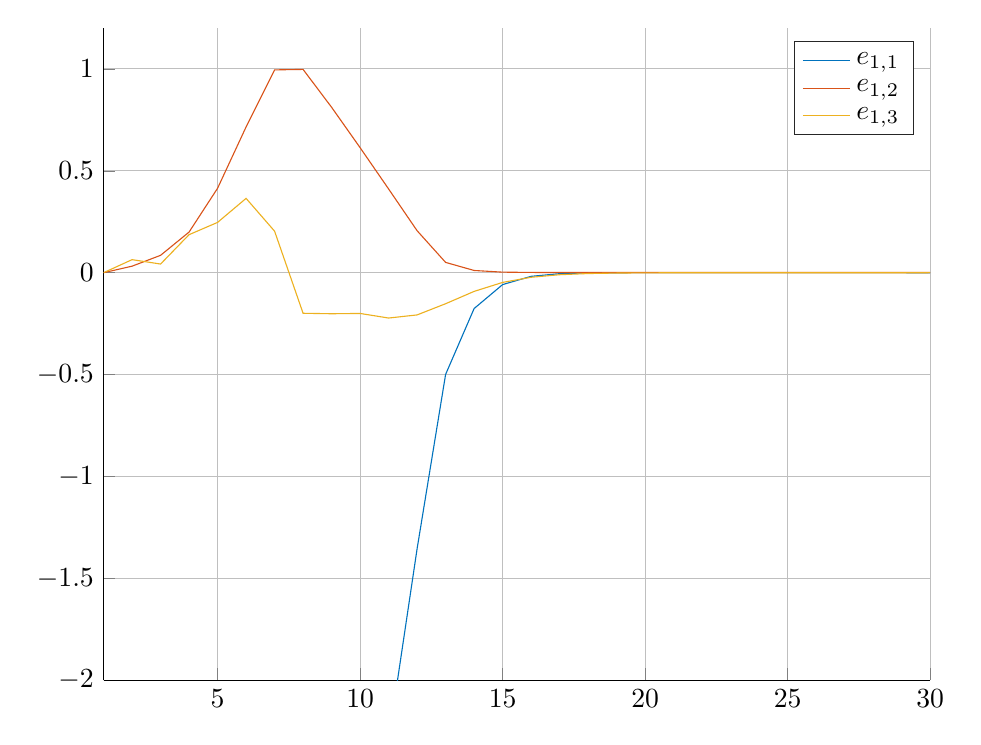
\begin{tikzpicture}

\begin{axis}[%
width=4.133in,
height=3.26in,
at={(0.693in,0.44in)},
scale only axis,
xmin=1,
xmax=30,
xmajorgrids,
ymin=-2,
ymax=1.2,
ymajorgrids,
axis background/.style={fill=white},
axis x line*=bottom,
axis y line*=left,
legend style={legend cell align=left,align=left,draw=white!15!black}
]
\addplot [color=mycolor1,solid]
  table[row sep=crcr]{%
1	-12\\
2	-11.0006833735421\\
3	-10.0021192569155\\
4	-9.00952868145095\\
5	-8.03306914168459\\
6	-7.08001255623633\\
7	-6.12118180980345\\
8	-5.12793789353629\\
9	-4.21288200406951\\
10	-3.23894935455442\\
11	-2.29381442313472\\
12	-1.35487988394669\\
13	-0.499312370868519\\
14	-0.17596074433855\\
15	-0.0583802953756676\\
16	-0.0178259942366529\\
17	-0.00479617368016515\\
18	-0.00100428938458844\\
19	-7.92867289323899e-05\\
20	9.29649554973803e-05\\
21	8.73608233178028e-05\\
22	6.3625304864517e-05\\
23	3.60834031070347e-05\\
24	4.22999112045958e-06\\
25	1.98254625995652e-05\\
26	2.94828838248126e-05\\
27	2.94728280518329e-05\\
28	1.50531071690665e-05\\
29	-8.67505865450849e-06\\
30	-3.09079933818332e-05\\
};
\addlegendentry{$\text{e}_\text{1,1}$};

\addplot [color=mycolor2,solid]
  table[row sep=crcr]{%
1	0\\
2	0.0320089043485361\\
3	0.0852138256801054\\
4	0.199375589105613\\
5	0.414373986327187\\
6	0.715248593560893\\
7	0.995404327740388\\
8	0.997692946624386\\
9	0.811883895891375\\
10	0.613694322145585\\
11	0.410968389749072\\
12	0.206034832263042\\
13	0.0505434736849072\\
14	0.0108779676275331\\
15	0.00266359315535002\\
16	0.00124055914570324\\
17	0.00102964127686267\\
18	0.00100293903841336\\
19	0.00100019690628069\\
20	0.000999982577653701\\
21	0.000999985526528874\\
22	0.000999991627214393\\
23	0.000999996118461188\\
24	0.000999999756480551\\
25	0.000999998511400314\\
26	0.000999997861669874\\
27	0.000999997862221436\\
28	0.000999998403503179\\
29	0.000999998976668245\\
30	0.000999999353061515\\
};
\addlegendentry{$\text{e}_\text{1,2}$};

\addplot [color=mycolor3,solid]
  table[row sep=crcr]{%
1	0\\
2	0.0640396917082695\\
3	0.0424224934033274\\
4	0.186599097136689\\
5	0.246847880346891\\
6	0.364736915409728\\
7	0.20380612469265\\
8	-0.199197760531278\\
9	-0.201469882549819\\
10	-0.200036173782283\\
11	-0.222549083116283\\
12	-0.207234440255294\\
13	-0.152322371123076\\
14	-0.0917977708064827\\
15	-0.0476990533762014\\
16	-0.022451354833858\\
17	-0.00992045698051751\\
18	-0.00416319906070547\\
19	-0.00176570089069606\\
20	-0.000722849709979919\\
21	-0.000329543347859896\\
22	-0.000184512024209963\\
23	-0.000141627165085949\\
24	-8.67954194984661e-05\\
25	-7.28766026362062e-05\\
26	-6.16790771800063e-05\\
27	-4.80214520712035e-05\\
28	-2.70537518430345e-05\\
29	-2.12571938586704e-05\\
30	-1.26018783145844e-05\\
};
\addlegendentry{$\text{e}_\text{1,3}$};

\end{axis}
\end{tikzpicture}%
}
      \caption{The evolution of the error states of agent 1 over time.}
      \label{fig:d_OFF_2_1_errors_agent_1}
    \end{figure}
  \end{minipage}
  \hfill
  \begin{minipage}{0.45\linewidth}
    \begin{figure}[H]
      \scalebox{0.7}{% This file was created by matlab2tikz.
%
%The latest updates can be retrieved from
%  http://www.mathworks.com/matlabcentral/fileexchange/22022-matlab2tikz-matlab2tikz
%where you can also make suggestions and rate matlab2tikz.
%
\definecolor{mycolor1}{rgb}{0.00000,0.44700,0.74100}%
\definecolor{mycolor2}{rgb}{0.85000,0.32500,0.09800}%
\definecolor{mycolor3}{rgb}{0.92900,0.69400,0.12500}%
%
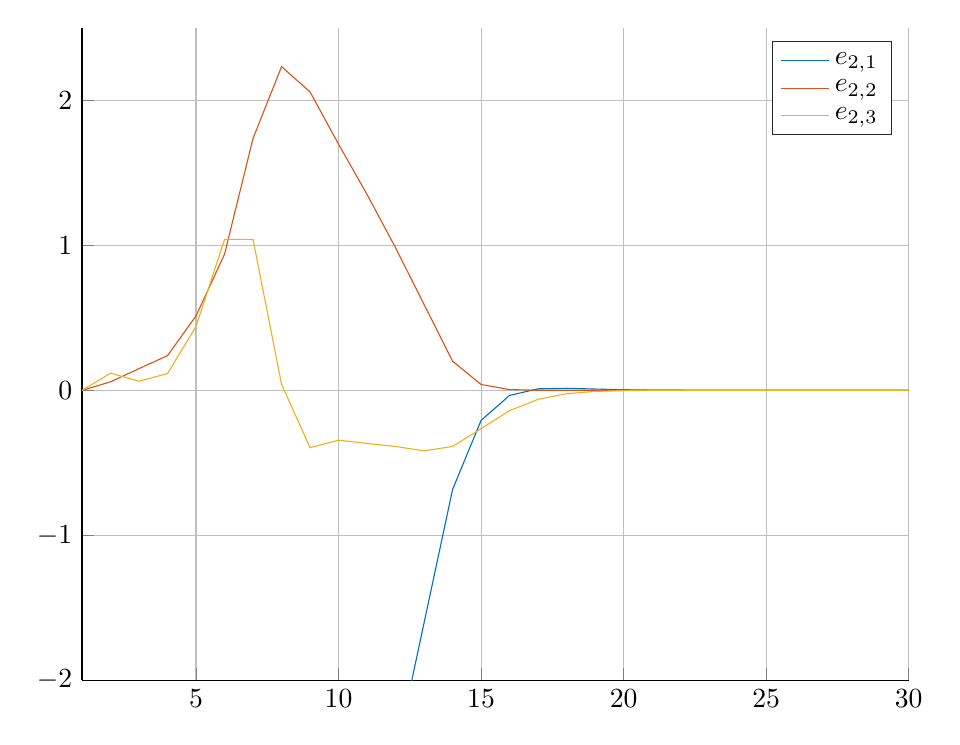
\begin{tikzpicture}

\begin{axis}[%
width=4.133in,
height=3.26in,
at={(0.693in,0.44in)},
scale only axis,
xmin=1,
xmax=30,
xmajorgrids,
ymin=-2,
ymax=2.5,
ymajorgrids,
axis background/.style={fill=white},
axis x line*=bottom,
axis y line*=left,
legend style={legend cell align=left,align=left,draw=white!15!black}
]
\addplot [color=mycolor1,solid]
  table[row sep=crcr]{%
1	-12\\
2	-11.0023543905482\\
3	-10.006633434098\\
4	-9.01079704287115\\
5	-8.05373409775359\\
6	-7.58951514106204\\
7	-7.12254347296275\\
8	-6.30103627329267\\
9	-5.32442964531907\\
10	-4.39195644766098\\
11	-3.45418687407344\\
12	-2.52424168800994\\
13	-1.60401940253906\\
14	-0.683756917507782\\
15	-0.206837932006062\\
16	-0.0343817016954163\\
17	0.0110504491347018\\
18	0.0146963776804634\\
19	0.00939565480365271\\
20	0.00467844056058416\\
21	0.0020231487474906\\
22	0.000836464053369204\\
23	0.000411158660101602\\
24	0.000212384021320647\\
25	0.00010071204771539\\
26	1.5906636794138e-05\\
27	-2.69577208067281e-05\\
28	-7.32138947398057e-05\\
29	-9.73583652783614e-05\\
30	-0.000122637500464277\\
};
\addlegendentry{$\text{e}_\text{2,1}$};

\addplot [color=mycolor2,solid]
  table[row sep=crcr]{%
1	0\\
2	0.0593781547176481\\
3	0.150390136386658\\
4	0.240247261648937\\
5	0.514568112733739\\
6	0.940360335286728\\
7	1.74012988352587\\
8	2.23462084315402\\
9	2.06021401055768\\
10	1.69928625125649\\
11	1.352088930889\\
12	0.984442050842019\\
13	0.593140929399552\\
14	0.201935686522527\\
15	0.0409765233814264\\
16	0.00564853745900544\\
17	0.0010543641591816\\
18	0.000900553799161971\\
19	0.000979193179093449\\
20	0.000998683427749768\\
21	0.00100047065422177\\
22	0.0010002629692842\\
23	0.00100014560046129\\
24	0.00100009762872017\\
25	0.00100007335059384\\
26	0.0010000566329609\\
27	0.00100004877485187\\
28	0.00100004071316151\\
29	0.0010000366874801\\
30	0.00100003259230527\\
};
\addlegendentry{$\text{e}_\text{2,2}$};

\addplot [color=mycolor3,solid]
  table[row sep=crcr]{%
1	0\\
2	0.118896306588512\\
3	0.0634033427941669\\
4	0.116574893449172\\
5	0.441713165288837\\
6	1.04278563123175\\
7	1.04183842017924\\
8	0.0418384201792416\\
9	-0.39528151932589\\
10	-0.343330567727176\\
11	-0.365846774431334\\
12	-0.38712298036403\\
13	-0.416998701650185\\
14	-0.386915045338552\\
15	-0.264072921211995\\
16	-0.140040004229625\\
17	-0.0615181094071543\\
18	-0.0228056551842437\\
19	-0.00686335907869728\\
20	-0.00140005095357263\\
21	5.38891544872821e-05\\
22	0.000296136318123524\\
23	0.000255790940646248\\
24	0.000226883715349592\\
25	0.000207927726798903\\
26	0.000186330906925296\\
27	0.000180319120463894\\
28	0.000168247982566255\\
29	0.00016521813070758\\
30	0.000158778300449284\\
};
\addlegendentry{$\text{e}_\text{2,3}$};

\end{axis}
\end{tikzpicture}%
}
      \caption{The evolution of the error states of agent 2 over time.}
      \label{fig:d_OFF_e2_1_errors_agent_1}
    \end{figure}
  \end{minipage}
\end{minipage}
}


\subsection{Distances between actors}
\label{subsection:distances_2_1}

\noindent\makebox[\linewidth][c]{%
\begin{minipage}{\linewidth}
  \begin{minipage}{0.45\linewidth}
    \begin{figure}[H]
      \scalebox{0.7}{% This file was created by matlab2tikz.
%
%The latest updates can be retrieved from
%  http://www.mathworks.com/matlabcentral/fileexchange/22022-matlab2tikz-matlab2tikz
%where you can also make suggestions and rate matlab2tikz.
%
\definecolor{mycolor1}{rgb}{0.00000,1.00000,1.00000}%
%
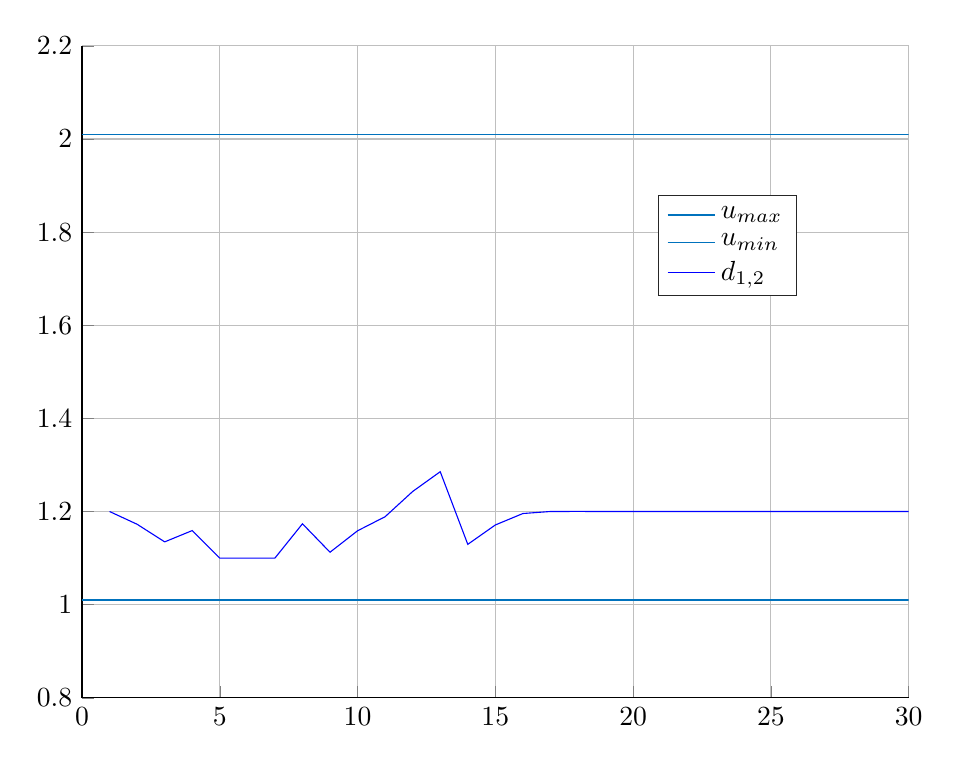
\begin{tikzpicture}

\begin{axis}[%
width=4.133in,
height=3.26in,
at={(0.693in,0.44in)},
scale only axis,
xmin=0,
xmax=30,
xmajorgrids,
ymin=0.8,
ymax=2.2,
ymajorgrids,
axis background/.style={fill=white},
axis x line*=bottom,
axis y line*=left,
legend style={at={(0.697,0.616)},anchor=south west,legend cell align=left,align=left,draw=white!15!black}
]
\addplot [color=mycolor1,solid]
  table[row sep=crcr]{%
0	1.01\\
30	1.01\\
};
\addlegendentry{$\text{u}_{\text{max}}$};

\addplot [color=mycolor1,solid]
  table[row sep=crcr]{%
0	2.01\\
30	2.01\\
};
\addlegendentry{$\text{u}_{\text{min}}$};

\addplot [color=blue,solid]
  table[row sep=crcr]{%
1	1.2\\
2	1.17263194024286\\
3	1.13483266765512\\
4	1.15912902140064\\
5	1.09999999999999\\
6	1.10000000002951\\
7	1.1\\
8	1.17367946140723\\
9	1.1125978423272\\
10	1.15866930719623\\
11	1.18889982720043\\
12	1.24303962211522\\
13	1.28551768990364\\
14	1.1295226779869\\
15	1.17113471383689\\
16	1.19570664201983\\
17	1.20007990615137\\
18	1.20020508497641\\
19	1.20005840853829\\
20	1.20001006018616\\
21	1.20000107623646\\
22	1.19999997752452\\
23	1.19999990913528\\
24	1.19999992018114\\
25	1.19999992788691\\
26	1.19999994130551\\
27	1.19999995041421\\
28	1.19999996093662\\
29	1.19999996556616\\
30	1.19999997026672\\
};
\addlegendentry{$\text{d}_{\text{1,2}}$};

\end{axis}
\end{tikzpicture}%}
      \caption{The distance between the two agents over time. The maximum allowed
        distance has a value of $2.1$ and the minimum allowed distance a value
        of $1.1$.}
      \label{fig:d_OFF_2_1_distance_agents}
    \end{figure}
  \end{minipage}
  \hfill
  \begin{minipage}{0.45\linewidth}
    \begin{figure}[H]
      \scalebox{0.7}{% This file was created by matlab2tikz.
%
%The latest updates can be retrieved from
%  http://www.mathworks.com/matlabcentral/fileexchange/22022-matlab2tikz-matlab2tikz
%where you can also make suggestions and rate matlab2tikz.
%
\definecolor{mycolor1}{rgb}{0.00000,0.44700,0.74100}%
\definecolor{mycolor2}{rgb}{0.85000,0.32500,0.09800}%
\definecolor{mycolor3}{rgb}{0.00000,1.00000,1.00000}%
%
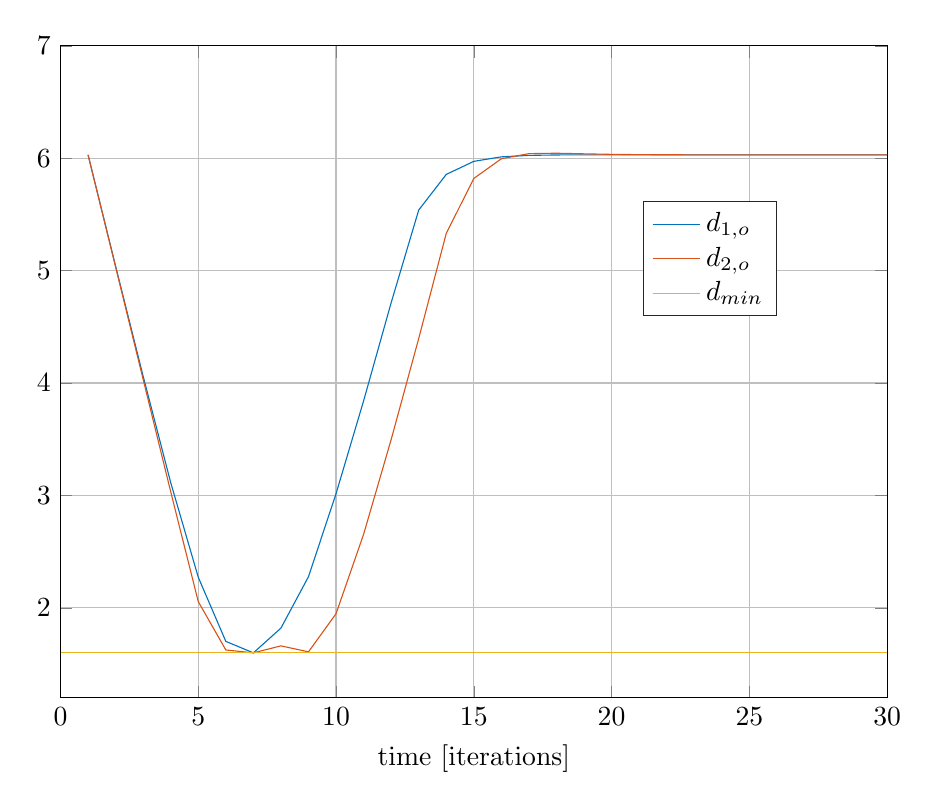
\begin{tikzpicture}

\begin{axis}[%
width=4.133in,
height=3.26in,
at={(0.693in,0.44in)},
scale only axis,
xmin=0,
xmax=30,
xmajorgrids,
ymin=1.2,
ymax=7,
ymajorgrids,
xlabel={time [iterations]},
axis background/.style={fill=white},
legend style={at={(0.705,0.585)},anchor=south west,legend cell align=left,align=left,draw=white!15!black}
]
\addplot [color=mycolor1,solid]
  table[row sep=crcr]{%
1	6.02992537267253\\
2	5.04046321855403\\
3	4.06035423743759\\
4	3.11388249889649\\
5	2.27207498093866\\
6	1.7018536906832\\
7	1.6\\
8	1.82019643698784\\
9	2.27754404279172\\
10	3.01603291996687\\
11	3.84159714379788\\
12	4.71453423398159\\
13	5.53902258565842\\
14	5.85598882707424\\
15	5.97210583637757\\
16	6.01231203824224\\
17	6.02525564178097\\
18	6.02902596351309\\
19	6.0299460861786\\
20	6.03011745882008\\
21	6.03011188288531\\
22	6.03008826615685\\
23	6.03006086183827\\
24	6.03002916739369\\
25	6.03004468508774\\
26	6.03005429435796\\
27	6.03005428435231\\
28	6.03003993648414\\
29	6.03001632652362\\
30	6.02999420433031\\
};
\addlegendentry{$\text{d}_{\text{1,o}}$};

\addplot [color=mycolor2,solid]
  table[row sep=crcr]{%
1	6.02992537267253\\
2	5.03148302473864\\
3	4.03178130665471\\
4	3.03221385560332\\
5	2.05551024119015\\
6	1.62554715142378\\
7	1.6\\
8	1.66210954473871\\
9	1.60891897271201\\
10	1.94787944401614\\
11	2.65458136663876\\
12	3.49695460848774\\
13	4.39598594857884\\
14	5.3311251823429\\
15	5.82007164848119\\
16	5.99515265377714\\
17	6.04081644951535\\
18	6.04445966667995\\
19	6.03917726706026\\
20	6.03448139874409\\
21	6.0318390491008\\
22	6.03065825207128\\
23	6.03023506163262\\
24	6.0300372748768\\
25	6.02992615766076\\
26	6.02984177338413\\
27	6.0297991218319\\
28	6.02975309526427\\
29	6.02972907062529\\
30	6.02970391694226\\
};
\addlegendentry{$\text{d}_{\text{2,o}}$};

\addplot [color=mycolor3,solid]
  table[row sep=crcr]{%
0	1.6\\
30	1.6\\
};
\addlegendentry{$\text{d}_{\text{min}}$};

\end{axis}
\end{tikzpicture}%
}
      \caption{The distance between each agent and the obstacle over time. The
        minimum allowed distance has a value of $1.6$.}
      \label{fig:d_OFF_2_1_distance_obstacle_agents}
    \end{figure}
  \end{minipage}
\end{minipage}
}


\subsection{Input signals}
\label{subsection:inputs_2_1}

\noindent\makebox[\linewidth][c]{%
\begin{minipage}{\linewidth}
  \begin{minipage}{0.45\linewidth}
    \begin{figure}[H]
      \scalebox{0.7}{% This file was created by matlab2tikz.
%
%The latest updates can be retrieved from
%  http://www.mathworks.com/matlabcentral/fileexchange/22022-matlab2tikz-matlab2tikz
%where you can also make suggestions and rate matlab2tikz.
%
\definecolor{mycolor1}{rgb}{0.00000,1.00000,1.00000}%
\definecolor{mycolor2}{rgb}{0.00000,0.44700,0.74100}%
\definecolor{mycolor3}{rgb}{0.85000,0.32500,0.09800}%
%
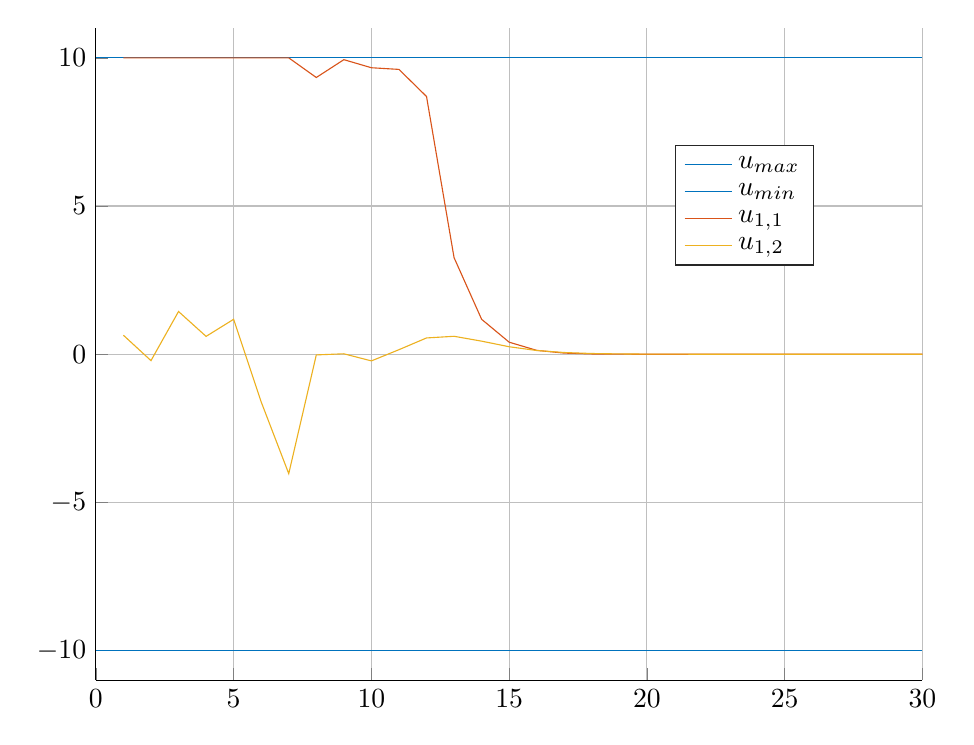
\begin{tikzpicture}

\begin{axis}[%
width=4.133in,
height=3.26in,
at={(0.693in,0.44in)},
scale only axis,
xmin=0,
xmax=30,
xmajorgrids,
ymin=-11,
ymax=11,
ymajorgrids,
axis background/.style={fill=white},
axis x line*=bottom,
axis y line*=left,
legend style={at={(0.701,0.636)},anchor=south west,legend cell align=left,align=left,draw=white!15!black}
]
\addplot [color=mycolor1,solid]
  table[row sep=crcr]{%
0	-10\\
30	-10\\
};
\addlegendentry{$\text{u}_{\text{max}}$};

\addplot [color=mycolor1,solid]
  table[row sep=crcr]{%
0	10\\
30	10\\
};
\addlegendentry{$\text{u}_{\text{min}}$};

\addplot [color=mycolor2,solid]
  table[row sep=crcr]{%
1	10\\
2	10\\
3	10\\
4	10\\
5	10\\
6	10\\
7	10\\
8	9.33730506764747\\
9	9.93893395762718\\
10	9.66652630248993\\
11	9.61048325332509\\
12	8.69691537476666\\
13	3.25825153669326\\
14	1.17876586137153\\
15	0.405803381179249\\
16	0.130316128031504\\
17	0.0379198354929674\\
18	0.00925006941654846\\
19	0.00172251825577133\\
20	-5.60413299154239e-05\\
21	-0.000237355192581102\\
22	-0.000275419021257852\\
23	-0.000318534121983164\\
24	0.000155954715289323\\
25	9.65742124715393e-05\\
26	-1.00557729949656e-07\\
27	-0.000144197208931895\\
28	-0.000237281658305302\\
29	-0.000222329347305799\\
30	-9.01400136149396e-05\\
};
\addlegendentry{$\text{u}_{\text{1,1}}$};

\addplot [color=mycolor3,solid]
  table[row sep=crcr]{%
1	0.640396917082695\\
2	-0.216171983049422\\
3	1.44176603733362\\
4	0.602487832102019\\
5	1.17889035062837\\
6	-1.60930790717078\\
7	-4.03003885223929\\
8	-0.0227212201854031\\
9	0.0143370876753578\\
10	-0.225129093340004\\
11	0.153146428609891\\
12	0.549120691322177\\
13	0.605246003165934\\
14	0.440987174302813\\
15	0.252476985423435\\
16	0.125308978533404\\
17	0.0575725791981203\\
18	0.0239749817000941\\
19	0.0104285118071614\\
20	0.00393306362120024\\
21	0.0014503132364993\\
22	0.000428848591240132\\
23	0.000548317455874824\\
24	0.000139188168622595\\
25	0.000111975254561998\\
26	0.000136576251088025\\
27	0.000209677002281687\\
28	5.79655798436393e-05\\
29	8.65531554408585e-05\\
30	-4.56767483585251e-05\\
};
\addlegendentry{$\text{u}_{\text{1,2}}$};

\end{axis}
\end{tikzpicture}%}
      \caption{The inputs signals directing agent 1 over time. Their value is
        constrained between $-10$ and $10$.}
      \label{fig:d_OFF_2_1_inputs_agent_1}
    \end{figure}
  \end{minipage}
  \hfill
  \begin{minipage}{0.45\linewidth}
    \begin{figure}[H]
      \scalebox{0.7}{% This file was created by matlab2tikz.
%
%The latest updates can be retrieved from
%  http://www.mathworks.com/matlabcentral/fileexchange/22022-matlab2tikz-matlab2tikz
%where you can also make suggestions and rate matlab2tikz.
%
\definecolor{mycolor1}{rgb}{0.00000,0.44700,0.74100}%
\definecolor{mycolor2}{rgb}{0.85000,0.32500,0.09800}%
%
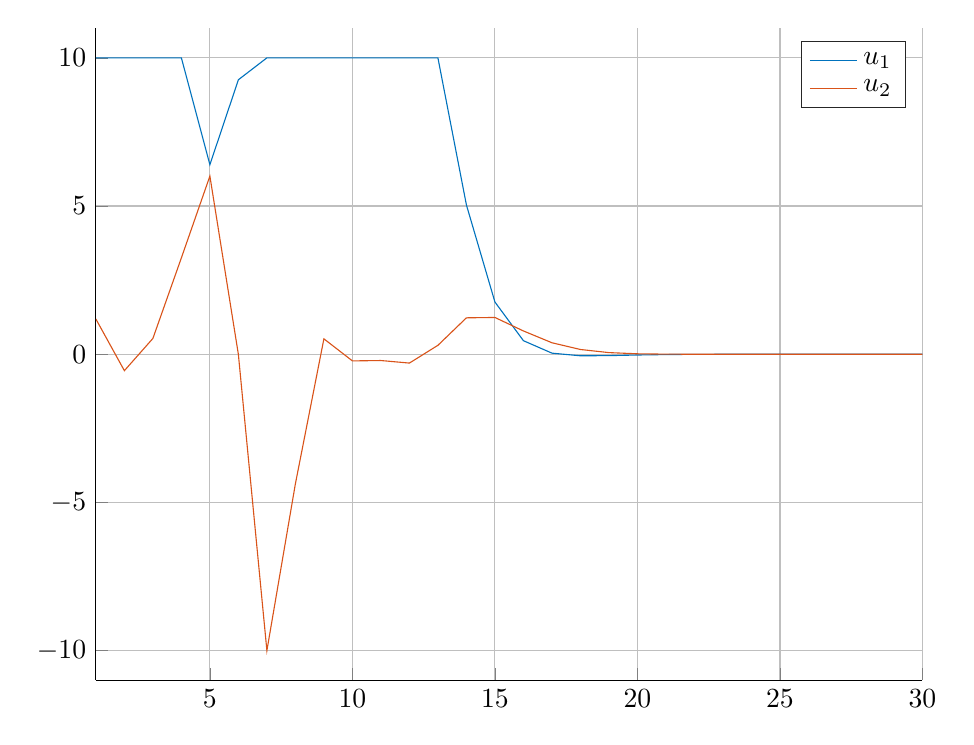
\begin{tikzpicture}

\begin{axis}[%
width=4.133in,
height=3.26in,
at={(0.693in,0.44in)},
scale only axis,
xmin=1,
xmax=30,
xmajorgrids,
ymin=-11,
ymax=11,
ymajorgrids,
axis background/.style={fill=white},
axis x line*=bottom,
axis y line*=left,
legend style={legend cell align=left,align=left,draw=white!15!black}
]
\addplot [color=mycolor1,solid]
  table[row sep=crcr]{%
1	10\\
2	10\\
3	10\\
4	10\\
5	6.39502727333906\\
6	9.26117667051881\\
7	10\\
8	10\\
9	10\\
10	10\\
11	10\\
12	10\\
13	10\\
14	5.03664982982595\\
15	1.76150438951348\\
16	0.456755785072588\\
17	0.0364939937185682\\
18	-0.053013623162716\\
19	-0.0471726037375023\\
20	-0.0265529264844818\\
21	-0.0118668471519676\\
22	-0.00425305409491201\\
23	-0.00198774644576558\\
24	-0.00111671976246029\\
25	-0.000848054125706662\\
26	-0.000428643583212237\\
27	-0.000462561746358677\\
28	-0.000241444708741716\\
29	-0.000252791355176646\\
30	-0.000105560470847361\\
};
\addlegendentry{$\text{u}_\text{1}$};

\addplot [color=mycolor2,solid]
  table[row sep=crcr]{%
1	1.18896306588512\\
2	-0.554929637943449\\
3	0.531715506550048\\
4	3.25138271839666\\
5	6.01072465942911\\
6	-0.00947211052508098\\
7	-10\\
8	-4.37119939505131\\
9	0.519509515987139\\
10	-0.225162067041581\\
11	-0.212762059326957\\
12	-0.29875721286155\\
13	0.30083656311633\\
14	1.22842124126557\\
15	1.2403291698237\\
16	0.785218948224705\\
17	0.387124542229106\\
18	0.159422961055464\\
19	0.0546330812512465\\
20	0.0145394010805992\\
21	0.00242247163636238\\
22	-0.000403453774772748\\
23	-0.000289072252966553\\
24	-0.000189559885506888\\
25	-0.00021596819873607\\
26	-6.01178646140153e-05\\
27	-0.000120711378976395\\
28	-3.02985185867415e-05\\
29	-6.43983025829581e-05\\
30	-8.76032382184133e-06\\
};
\addlegendentry{$\text{u}_\text{2}$};

\end{axis}
\end{tikzpicture}%}
      \caption{The inputs signals directing agent 2 over time. Their value is
        constrained between $-10$ and $10$.}
      \label{fig:d_OFF_2_1_inputs_agent_2}
    \end{figure}
  \end{minipage}
\end{minipage}
}
